% **************************************************************************************************************
% A Classic Thesis Style
% An Homage to The Elements of Typographic Style
%
% Copyright (C) 2012 Andr\'e Miede http://www.miede.de
%
% If you like the style then I would appreciate a postcard. My address
% can be found in the file ClassicThesis.pdf. A collection of the
% postcards I received so far is available online at
% http://postcards.miede.de
%
% License:
% This program is free software; you can redistribute it and/or modify
% it under the terms of the GNU General Public License as published by
% the Free Software Foundation; either version 2 of the License, or
% (at your option) any later version.
%
% This program is distributed in the hope that it will be useful,
% but WITHOUT ANY WARRANTY; without even the implied warranty of
% MERCHANTABILITY or FITNESS FOR A PARTICULAR PURPOSE.  See the
% GNU General Public License for more details.
%
% You should have received a copy of the GNU General Public License
% along with this program; see the file COPYING.  If not, write to
% the Free Software Foundation, Inc., 59 Temple Place - Suite 330,
% Boston, MA 02111-1307, USA.
%
% **************************************************************************************************************
% Note:
%    * You must not use "u etc. in strings/commands that will be spaced out (use \"u or real umlauts instead)
%    * New enumeration (small caps): \begin{aenumerate} \end{aenumerate}
%    * For margin notes: \marginpar or \graffito{}
%    * Do not use bold fonts in this style, it is designed around them
%    * Use tables as in the examples
%    * See classicthesis-preamble.sty for useful commands
% **************************************************************************************************************
% To Do:
%                * [high] Check this out: http://www.golatex.de/koma-script-warnung-in-verbindung-mit-listings-package-t2058.html
%    * [medium] mathbb in section-titles/chapter-titles => disappears somehow in headlines!!!
% **************************************************************************************************************
\documentclass[ twoside,openright,titlepage,numbers=noenddot,headinclude,%1headlines,% letterpaper a4paper
                footinclude=true,cleardoublepage=empty,abstractoff, % <--- obsolete, remove (todo)
                BCOR=5mm,paper=a4,fontsize=11pt,%11pt,a4paper,%
                american,%draft%
                ]{scrreprt}

% TODO: Remove draft option!!

%********************************************************************
% Note: Make all your adjustments in here
%*******************************************************
% ****************************************************************************************************
% classicthesis-config.tex
% formerly known as loadpackages.sty, classicthesis-ldpkg.sty, and classicthesis-preamble.sty
% Use it at the beginning of your ClassicThesis.tex, or as a LaTeX Preamble
% in your ClassicThesis.{tex,lyx} with % ****************************************************************************************************
% classicthesis-config.tex
% formerly known as loadpackages.sty, classicthesis-ldpkg.sty, and classicthesis-preamble.sty
% Use it at the beginning of your ClassicThesis.tex, or as a LaTeX Preamble
% in your ClassicThesis.{tex,lyx} with % ****************************************************************************************************
% classicthesis-config.tex
% formerly known as loadpackages.sty, classicthesis-ldpkg.sty, and classicthesis-preamble.sty
% Use it at the beginning of your ClassicThesis.tex, or as a LaTeX Preamble
% in your ClassicThesis.{tex,lyx} with \input{classicthesis-config}
% ****************************************************************************************************
% If you like the classicthesis, then I would appreciate a postcard.
% My address can be found in the file ClassicThesis.pdf. A collection
% of the postcards I received so far is available online at
% http://postcards.miede.de
% ****************************************************************************************************

\usepackage[dvipsnames]{xcolor}

\usepackage[centerlast]{caption}
\captionsetup{font=small}

\usepackage{subcaption}
\expandafter\def\csname ver@subfig.sty\endcsname{}

\usepackage{fancyvrb}
\usepackage{setspace}

\newenvironment{CVerbatim}
 {\singlespacing\center\BVerbatim}
 {\endBVerbatim\endcenter}

\usepackage[utf8]{inputenc}

% ****************************************************************************************************
% 1. Configure classicthesis for your needs here, e.g., remove "drafting" below
% in order to deactivate the time-stamp on the pages
% ****************************************************************************************************
\PassOptionsToPackage{listings,%
                                 pdfspacing,%floatperchapter,%linedheaders,%
                                 subfig,beramono,eulermath,parts,dottedtoc,eulermath}{classicthesis}
% ********************************************************************
% Available options for classicthesis.sty
% (see ClassicThesis.pdf for more information):
% drafting
% parts nochapters linedheaders
% eulerchapternumbers beramono eulermath pdfspacing minionprospacing
% tocaligned dottedtoc manychapters
% listings floatperchapter subfig
% ********************************************************************

% ********************************************************************
% Triggers for this config
% ********************************************************************
\usepackage{ifthen}
\newboolean{enable-backrefs} % enable backrefs in the bibliography
\setboolean{enable-backrefs}{false} % true false
% ****************************************************************************************************


% ****************************************************************************************************
% 2. Personal data and user ad-hoc commands
% * <klara.seitz@googlemail.com> 2016-05-03T10:24:37.032Z:
%
% > 2. Personal data and user ad-hoc commands
%
% Add our own data
%
% ^.
% ****************************************************************************************************
\newcommand{\myTitle}{Platener: Generating 2D~Laser Cuttable Construction Plans from 3D~Models \xspace}
\newcommand{\mySubtitle}{A thesis submitted in partial fulfillment of the requirements for the degree of\xspace}
\newcommand{\myDegree}{\emph{Bachelor of Science in IT Systems Engineering}\xspace}
\newcommand{\myName}{Daniel-Amadeus J. Glöckner,\xspace
Sven Mischkewitz,\xspace
Dimitri Schmidt,\xspace
Klara Seitz,\xspace
Lukas Wagner
\xspace}
\newcommand{\myProf}{Prof. Dr. Patrick Baudisch\xspace}
%\newcommand{\myOtherProf}{Put name here\xspace}
\newcommand{\mySupervisor}{Stefanie Müller\xspace}
\newcommand{\myFaculty}{Hasso Plattner Institute\xspace}
\newcommand{\myDepartment}{Human-Computer Interaction Group\xspace}
\newcommand{\myUni}{University of Potsdam\xspace}
\newcommand{\myLocation}{Potsdam\xspace}
\newcommand{\myTime}{July 2016\xspace}
%\newcommand{\myVersion}{version 4.1\xspace}

% ********************************************************************
% Setup, finetuning, and useful commands
% ********************************************************************
\newcounter{dummy} % necessary for correct hyperlinks (to index, bib, etc.)
\newlength{\abcd} % for ab..z string length calculation
\providecommand{\mLyX}{L\kern-.1667em\lower.25em\hbox{Y}\kern-.125emX\@}
\newcommand{\ie}{i.\,e.}
\newcommand{\Ie}{I.\,e.}
\newcommand{\eg}{e.\,g.}
\newcommand{\Eg}{E.\,g.}
% ****************************************************************************************************


% ****************************************************************************************************
% 3. Loading some handy packages
% ****************************************************************************************************
% ********************************************************************
% Packages with options that might require adjustments
% ********************************************************************
\PassOptionsToPackage{latin9}{inputenc}	% latin9 (ISO-8859-9) = latin1+"Euro sign"
 \usepackage{inputenc}

%\PassOptionsToPackage{ngerman,american}{babel}   % change this to your language(s)
% Spanish languages need extra options in order to work with this template
%\PassOptionsToPackage{spanish,es-lcroman}{babel}
 \usepackage{babel}

\PassOptionsToPackage{square,numbers}{natbib}
\usepackage{natbib}

\PassOptionsToPackage{fleqn}{amsmath}		% math environments and more by the AMS
 \usepackage{amsmath}

% ********************************************************************
% General useful packages
% ********************************************************************
\PassOptionsToPackage{T1}{fontenc} % T2A for cyrillics
        \usepackage{fontenc}
\usepackage{textcomp} % fix warning with missing font shapes
\usepackage{xspace} % to get the spacing after macros right
\usepackage{mparhack} % get marginpar right
\usepackage{fixltx2e} % fixes some LaTeX stuff
\PassOptionsToPackage{printonlyused,smaller}{acronym}
        \usepackage{acronym} % nice macros for handling all acronyms in the thesis
%\renewcommand*{\acsfont}[1]{\textssc{#1}} % for MinionPro
\renewcommand{\aclabelfont}[1]{{#1}\hfill} % fix the list of acronyms
% ****************************************************************************************************


% ****************************************************************************************************
% 4. Setup floats: tables, (sub)figures, and captions
% ****************************************************************************************************
\usepackage{tabularx} % better tables
        \setlength{\extrarowheight}{3pt} % increase table row height
\newcommand{\tableheadline}[1]{\multicolumn{1}{c}{\spacedlowsmallcaps{#1}}}
\newcommand{\myfloatalign}{\centering} % to be used with each float for alignment


% \usepackage{subfig}
% \usepackage[lofdepth,lotdepth]{subfig}
%\usepackage{subcaption}


% ****************************************************************************************************


% ****************************************************************************************************
% 5. Setup code listings
% ****************************************************************************************************
\usepackage{listings}
\usepackage{minted}
\usemintedstyle{pastie}
\usepackage{scrhack} % fix warnings when using KOMA with listings package


%\lstset{emph={trueIndex,root},emphstyle=\color{BlueViolet}}%\underbar} % for special keywords
\lstset{language=[LaTeX]Tex,%C++,
    keywordstyle=\color{RoyalBlue},%\bfseries,
    basicstyle=\small\ttfamily,
    %identifierstyle=\color{NavyBlue},
    commentstyle=\color{Green}\ttfamily,
    stringstyle=\rmfamily,
    numbers=none,%left,%
    numberstyle=\scriptsize,%\tiny
    stepnumber=5,
    numbersep=8pt,
    showstringspaces=false,
    breaklines=true,
    frameround=ftff,
    frame=single,
    belowcaptionskip=.75\baselineskip
    %frame=L
}
% ****************************************************************************************************


% ****************************************************************************************************
% 6. PDFLaTeX, hyperreferences and citation backreferences
% ****************************************************************************************************
% ********************************************************************
% Using PDFLaTeX
% ********************************************************************
\PassOptionsToPackage{pdftex,hyperfootnotes=false,pdfpagelabels}{hyperref}
        \usepackage{hyperref}  % backref linktocpage pagebackref
\pdfcompresslevel=9
\pdfadjustspacing=1
\PassOptionsToPackage{pdftex}{graphicx}
        \usepackage{graphicx}
        \DeclareGraphicsExtensions{.pdf,.png,.jpg,.ai}
    \DeclareGraphicsRule{.ai}{pdf}{.ai}{}
    \graphicspath{{Images/}{../Images/}}
    \usepackage{svg}

% ********************************************************************
% Setup the style of the backrefs from the bibliography
% (translate the options to any language you use)
% ********************************************************************
\newcommand{\backrefnotcitedstring}{\relax}%(Not cited.)
\newcommand{\backrefcitedsinglestring}[1]{(Cited on page~#1.)}
\newcommand{\backrefcitedmultistring}[1]{(Cited on pages~#1.)}
\ifthenelse{\boolean{enable-backrefs}}%
{%
                \PassOptionsToPackage{hyperpageref}{backref}
                \usepackage{backref} % to be loaded after hyperref package
                   \renewcommand{\backreftwosep}{ and~} % separate 2 pages
                   \renewcommand{\backreflastsep}{, and~} % separate last of longer list
                   \renewcommand*{\backref}[1]{}  % disable standard
                   \renewcommand*{\backrefalt}[4]{% detailed backref
                      \ifcase #1 %
                         \backrefnotcitedstring%
                      \or%
                         \backrefcitedsinglestring{#2}%
                      \else%
                         \backrefcitedmultistring{#2}%
                      \fi}%
}{\relax}

% ********************************************************************
% Hyperreferences
% ********************************************************************
\hypersetup{%
    %draft,	% = no hyperlinking at all (useful in b/w printouts)
    colorlinks=true, linktocpage=true, pdfstartpage=3, pdfstartview=FitV,%
    % uncomment the following line if you want to have black links (e.g., for printing)
    %colorlinks=false, linktocpage=false, pdfborder={0 0 0}, pdfstartpage=3, pdfstartview=FitV,%
    breaklinks=true, pdfpagemode=UseNone, pageanchor=true, pdfpagemode=UseOutlines,%
    plainpages=false, bookmarksnumbered, bookmarksopen=true, bookmarksopenlevel=1,%
    hypertexnames=true, pdfhighlight=/O,%nesting=true,%frenchlinks,%
    urlcolor=webbrown, linkcolor=RoyalBlue, citecolor=webgreen, %pagecolor=RoyalBlue,%
    %urlcolor=Black, linkcolor=Black, citecolor=Black, %pagecolor=Black,%
    pdftitle={\myTitle},%
    pdfauthor={\textcopyright\ \myName, \myUni, \myFaculty},%
    pdfsubject={},%
    pdfkeywords={},%
    pdfcreator={pdfLaTeX},%
    pdfproducer={LaTeX with hyperref and classicthesis}%
}

% ********************************************************************
% Setup autoreferences
% ********************************************************************
% There are some issues regarding autorefnames
% http://www.ureader.de/msg/136221647.aspx
% http://www.tex.ac.uk/cgi-bin/texfaq2html?label=latexwords
% you have to redefine the makros for the
% language you use, e.g., american, ngerman
% (as chosen when loading babel/AtBeginDocument)
% ********************************************************************
\makeatletter
\@ifpackageloaded{babel}%
    {%
       \addto\extrasamerican{%
                                        \renewcommand*{\figureautorefname}{Figure}%
                                        \renewcommand*{\tableautorefname}{Table}%
                                        \renewcommand*{\partautorefname}{Part}%
                                        \renewcommand*{\chapterautorefname}{Chapter}%
                                        \renewcommand*{\sectionautorefname}{Section}%
                                        \renewcommand*{\subsectionautorefname}{Section}%
                                        \renewcommand*{\subsubsectionautorefname}{Section}%
                                }%
       \addto\extrasngerman{%
                                        \renewcommand*{\paragraphautorefname}{Absatz}%
                                        \renewcommand*{\subparagraphautorefname}{Unterabsatz}%
                                        \renewcommand*{\footnoteautorefname}{Fu\"snote}%
                                        \renewcommand*{\FancyVerbLineautorefname}{Zeile}%
                                        \renewcommand*{\theoremautorefname}{Theorem}%
                                        \renewcommand*{\appendixautorefname}{Anhang}%
                                        \renewcommand*{\equationautorefname}{Gleichung}%
                                        \renewcommand*{\itemautorefname}{Punkt}%
                                }%
                        % Fix to getting autorefs for subfigures right (thanks to Belinda Vogt for changing the definition)
                        \providecommand{\subfigureautorefname}{\figureautorefname}%
    }{\relax}
\makeatother


% ****************************************************************************************************
% 7. Last calls before the bar closes
% ****************************************************************************************************
% ********************************************************************
% Development Stuff
% ********************************************************************
\listfiles
%\PassOptionsToPackage{l2tabu,orthodox,abort}{nag}
%	\usepackage{nag}
%\PassOptionsToPackage{warning, all}{onlyamsmath}
%	\usepackage{onlyamsmath}

% ********************************************************************
% Last, but not least...
% ********************************************************************
\usepackage{classicthesis}
% ****************************************************************************************************


% ****************************************************************************************************
% 8. Further adjustments (experimental)
% ****************************************************************************************************
% ********************************************************************
% Changing the text area
% ********************************************************************
%\linespread{1.05} % a bit more for Palatino
%\areaset[current]{312pt}{761pt} % 686 (factor 2.2) + 33 head + 42 head \the\footskip
%\setlength{\marginparwidth}{7em}%
%\setlength{\marginparsep}{2em}%

\setlength{\intextsep}{32pt}

% ********************************************************************
% Using different fonts
% ********************************************************************
%\usepackage[oldstylenums]{kpfonts} % oldstyle notextcomp
%\usepackage[osf]{libertine}
%\usepackage{hfoldsty} % Computer Modern with osf
%\usepackage[light,condensed,math]{iwona}
%\renewcommand{\sfdefault}{iwona}
%\usepackage{lmodern} % <-- no osf support :-(
%\usepackage[urw-garamond]{mathdesign} <-- no osf support :-(
% ****************************************************************************************************

%%% Local Variables:
%%% mode: latex
%%% TeX-command-extra-options: "-shell-escape"
%%% End:

% ****************************************************************************************************
% If you like the classicthesis, then I would appreciate a postcard.
% My address can be found in the file ClassicThesis.pdf. A collection
% of the postcards I received so far is available online at
% http://postcards.miede.de
% ****************************************************************************************************

\usepackage[dvipsnames]{xcolor}

\usepackage[centerlast]{caption}
\captionsetup{font=small}

\usepackage{subcaption}
\expandafter\def\csname ver@subfig.sty\endcsname{}

\usepackage{fancyvrb}
\usepackage{setspace}

\newenvironment{CVerbatim}
 {\singlespacing\center\BVerbatim}
 {\endBVerbatim\endcenter}

\usepackage[utf8]{inputenc}

% ****************************************************************************************************
% 1. Configure classicthesis for your needs here, e.g., remove "drafting" below
% in order to deactivate the time-stamp on the pages
% ****************************************************************************************************
\PassOptionsToPackage{listings,%
                                 pdfspacing,%floatperchapter,%linedheaders,%
                                 subfig,beramono,eulermath,parts,dottedtoc,eulermath}{classicthesis}
% ********************************************************************
% Available options for classicthesis.sty
% (see ClassicThesis.pdf for more information):
% drafting
% parts nochapters linedheaders
% eulerchapternumbers beramono eulermath pdfspacing minionprospacing
% tocaligned dottedtoc manychapters
% listings floatperchapter subfig
% ********************************************************************

% ********************************************************************
% Triggers for this config
% ********************************************************************
\usepackage{ifthen}
\newboolean{enable-backrefs} % enable backrefs in the bibliography
\setboolean{enable-backrefs}{false} % true false
% ****************************************************************************************************


% ****************************************************************************************************
% 2. Personal data and user ad-hoc commands
% * <klara.seitz@googlemail.com> 2016-05-03T10:24:37.032Z:
%
% > 2. Personal data and user ad-hoc commands
%
% Add our own data
%
% ^.
% ****************************************************************************************************
\newcommand{\myTitle}{Platener: Generating 2D~Laser Cuttable Construction Plans from 3D~Models \xspace}
\newcommand{\mySubtitle}{A thesis submitted in partial fulfillment of the requirements for the degree of\xspace}
\newcommand{\myDegree}{\emph{Bachelor of Science in IT Systems Engineering}\xspace}
\newcommand{\myName}{Daniel-Amadeus J. Glöckner,\xspace
Sven Mischkewitz,\xspace
Dimitri Schmidt,\xspace
Klara Seitz,\xspace
Lukas Wagner
\xspace}
\newcommand{\myProf}{Prof. Dr. Patrick Baudisch\xspace}
%\newcommand{\myOtherProf}{Put name here\xspace}
\newcommand{\mySupervisor}{Stefanie Müller\xspace}
\newcommand{\myFaculty}{Hasso Plattner Institute\xspace}
\newcommand{\myDepartment}{Human-Computer Interaction Group\xspace}
\newcommand{\myUni}{University of Potsdam\xspace}
\newcommand{\myLocation}{Potsdam\xspace}
\newcommand{\myTime}{July 2016\xspace}
%\newcommand{\myVersion}{version 4.1\xspace}

% ********************************************************************
% Setup, finetuning, and useful commands
% ********************************************************************
\newcounter{dummy} % necessary for correct hyperlinks (to index, bib, etc.)
\newlength{\abcd} % for ab..z string length calculation
\providecommand{\mLyX}{L\kern-.1667em\lower.25em\hbox{Y}\kern-.125emX\@}
\newcommand{\ie}{i.\,e.}
\newcommand{\Ie}{I.\,e.}
\newcommand{\eg}{e.\,g.}
\newcommand{\Eg}{E.\,g.}
% ****************************************************************************************************


% ****************************************************************************************************
% 3. Loading some handy packages
% ****************************************************************************************************
% ********************************************************************
% Packages with options that might require adjustments
% ********************************************************************
\PassOptionsToPackage{latin9}{inputenc}	% latin9 (ISO-8859-9) = latin1+"Euro sign"
 \usepackage{inputenc}

%\PassOptionsToPackage{ngerman,american}{babel}   % change this to your language(s)
% Spanish languages need extra options in order to work with this template
%\PassOptionsToPackage{spanish,es-lcroman}{babel}
 \usepackage{babel}

\PassOptionsToPackage{square,numbers}{natbib}
\usepackage{natbib}

\PassOptionsToPackage{fleqn}{amsmath}		% math environments and more by the AMS
 \usepackage{amsmath}

% ********************************************************************
% General useful packages
% ********************************************************************
\PassOptionsToPackage{T1}{fontenc} % T2A for cyrillics
        \usepackage{fontenc}
\usepackage{textcomp} % fix warning with missing font shapes
\usepackage{xspace} % to get the spacing after macros right
\usepackage{mparhack} % get marginpar right
\usepackage{fixltx2e} % fixes some LaTeX stuff
\PassOptionsToPackage{printonlyused,smaller}{acronym}
        \usepackage{acronym} % nice macros for handling all acronyms in the thesis
%\renewcommand*{\acsfont}[1]{\textssc{#1}} % for MinionPro
\renewcommand{\aclabelfont}[1]{{#1}\hfill} % fix the list of acronyms
% ****************************************************************************************************


% ****************************************************************************************************
% 4. Setup floats: tables, (sub)figures, and captions
% ****************************************************************************************************
\usepackage{tabularx} % better tables
        \setlength{\extrarowheight}{3pt} % increase table row height
\newcommand{\tableheadline}[1]{\multicolumn{1}{c}{\spacedlowsmallcaps{#1}}}
\newcommand{\myfloatalign}{\centering} % to be used with each float for alignment


% \usepackage{subfig}
% \usepackage[lofdepth,lotdepth]{subfig}
%\usepackage{subcaption}


% ****************************************************************************************************


% ****************************************************************************************************
% 5. Setup code listings
% ****************************************************************************************************
\usepackage{listings}
\usepackage{minted}
\usemintedstyle{pastie}
\usepackage{scrhack} % fix warnings when using KOMA with listings package


%\lstset{emph={trueIndex,root},emphstyle=\color{BlueViolet}}%\underbar} % for special keywords
\lstset{language=[LaTeX]Tex,%C++,
    keywordstyle=\color{RoyalBlue},%\bfseries,
    basicstyle=\small\ttfamily,
    %identifierstyle=\color{NavyBlue},
    commentstyle=\color{Green}\ttfamily,
    stringstyle=\rmfamily,
    numbers=none,%left,%
    numberstyle=\scriptsize,%\tiny
    stepnumber=5,
    numbersep=8pt,
    showstringspaces=false,
    breaklines=true,
    frameround=ftff,
    frame=single,
    belowcaptionskip=.75\baselineskip
    %frame=L
}
% ****************************************************************************************************


% ****************************************************************************************************
% 6. PDFLaTeX, hyperreferences and citation backreferences
% ****************************************************************************************************
% ********************************************************************
% Using PDFLaTeX
% ********************************************************************
\PassOptionsToPackage{pdftex,hyperfootnotes=false,pdfpagelabels}{hyperref}
        \usepackage{hyperref}  % backref linktocpage pagebackref
\pdfcompresslevel=9
\pdfadjustspacing=1
\PassOptionsToPackage{pdftex}{graphicx}
        \usepackage{graphicx}
        \DeclareGraphicsExtensions{.pdf,.png,.jpg,.ai}
    \DeclareGraphicsRule{.ai}{pdf}{.ai}{}
    \graphicspath{{Images/}{../Images/}}
    \usepackage{svg}

% ********************************************************************
% Setup the style of the backrefs from the bibliography
% (translate the options to any language you use)
% ********************************************************************
\newcommand{\backrefnotcitedstring}{\relax}%(Not cited.)
\newcommand{\backrefcitedsinglestring}[1]{(Cited on page~#1.)}
\newcommand{\backrefcitedmultistring}[1]{(Cited on pages~#1.)}
\ifthenelse{\boolean{enable-backrefs}}%
{%
                \PassOptionsToPackage{hyperpageref}{backref}
                \usepackage{backref} % to be loaded after hyperref package
                   \renewcommand{\backreftwosep}{ and~} % separate 2 pages
                   \renewcommand{\backreflastsep}{, and~} % separate last of longer list
                   \renewcommand*{\backref}[1]{}  % disable standard
                   \renewcommand*{\backrefalt}[4]{% detailed backref
                      \ifcase #1 %
                         \backrefnotcitedstring%
                      \or%
                         \backrefcitedsinglestring{#2}%
                      \else%
                         \backrefcitedmultistring{#2}%
                      \fi}%
}{\relax}

% ********************************************************************
% Hyperreferences
% ********************************************************************
\hypersetup{%
    %draft,	% = no hyperlinking at all (useful in b/w printouts)
    colorlinks=true, linktocpage=true, pdfstartpage=3, pdfstartview=FitV,%
    % uncomment the following line if you want to have black links (e.g., for printing)
    %colorlinks=false, linktocpage=false, pdfborder={0 0 0}, pdfstartpage=3, pdfstartview=FitV,%
    breaklinks=true, pdfpagemode=UseNone, pageanchor=true, pdfpagemode=UseOutlines,%
    plainpages=false, bookmarksnumbered, bookmarksopen=true, bookmarksopenlevel=1,%
    hypertexnames=true, pdfhighlight=/O,%nesting=true,%frenchlinks,%
    urlcolor=webbrown, linkcolor=RoyalBlue, citecolor=webgreen, %pagecolor=RoyalBlue,%
    %urlcolor=Black, linkcolor=Black, citecolor=Black, %pagecolor=Black,%
    pdftitle={\myTitle},%
    pdfauthor={\textcopyright\ \myName, \myUni, \myFaculty},%
    pdfsubject={},%
    pdfkeywords={},%
    pdfcreator={pdfLaTeX},%
    pdfproducer={LaTeX with hyperref and classicthesis}%
}

% ********************************************************************
% Setup autoreferences
% ********************************************************************
% There are some issues regarding autorefnames
% http://www.ureader.de/msg/136221647.aspx
% http://www.tex.ac.uk/cgi-bin/texfaq2html?label=latexwords
% you have to redefine the makros for the
% language you use, e.g., american, ngerman
% (as chosen when loading babel/AtBeginDocument)
% ********************************************************************
\makeatletter
\@ifpackageloaded{babel}%
    {%
       \addto\extrasamerican{%
                                        \renewcommand*{\figureautorefname}{Figure}%
                                        \renewcommand*{\tableautorefname}{Table}%
                                        \renewcommand*{\partautorefname}{Part}%
                                        \renewcommand*{\chapterautorefname}{Chapter}%
                                        \renewcommand*{\sectionautorefname}{Section}%
                                        \renewcommand*{\subsectionautorefname}{Section}%
                                        \renewcommand*{\subsubsectionautorefname}{Section}%
                                }%
       \addto\extrasngerman{%
                                        \renewcommand*{\paragraphautorefname}{Absatz}%
                                        \renewcommand*{\subparagraphautorefname}{Unterabsatz}%
                                        \renewcommand*{\footnoteautorefname}{Fu\"snote}%
                                        \renewcommand*{\FancyVerbLineautorefname}{Zeile}%
                                        \renewcommand*{\theoremautorefname}{Theorem}%
                                        \renewcommand*{\appendixautorefname}{Anhang}%
                                        \renewcommand*{\equationautorefname}{Gleichung}%
                                        \renewcommand*{\itemautorefname}{Punkt}%
                                }%
                        % Fix to getting autorefs for subfigures right (thanks to Belinda Vogt for changing the definition)
                        \providecommand{\subfigureautorefname}{\figureautorefname}%
    }{\relax}
\makeatother


% ****************************************************************************************************
% 7. Last calls before the bar closes
% ****************************************************************************************************
% ********************************************************************
% Development Stuff
% ********************************************************************
\listfiles
%\PassOptionsToPackage{l2tabu,orthodox,abort}{nag}
%	\usepackage{nag}
%\PassOptionsToPackage{warning, all}{onlyamsmath}
%	\usepackage{onlyamsmath}

% ********************************************************************
% Last, but not least...
% ********************************************************************
\usepackage{classicthesis}
% ****************************************************************************************************


% ****************************************************************************************************
% 8. Further adjustments (experimental)
% ****************************************************************************************************
% ********************************************************************
% Changing the text area
% ********************************************************************
%\linespread{1.05} % a bit more for Palatino
%\areaset[current]{312pt}{761pt} % 686 (factor 2.2) + 33 head + 42 head \the\footskip
%\setlength{\marginparwidth}{7em}%
%\setlength{\marginparsep}{2em}%

\setlength{\intextsep}{32pt}

% ********************************************************************
% Using different fonts
% ********************************************************************
%\usepackage[oldstylenums]{kpfonts} % oldstyle notextcomp
%\usepackage[osf]{libertine}
%\usepackage{hfoldsty} % Computer Modern with osf
%\usepackage[light,condensed,math]{iwona}
%\renewcommand{\sfdefault}{iwona}
%\usepackage{lmodern} % <-- no osf support :-(
%\usepackage[urw-garamond]{mathdesign} <-- no osf support :-(
% ****************************************************************************************************

%%% Local Variables:
%%% mode: latex
%%% TeX-command-extra-options: "-shell-escape"
%%% End:

% ****************************************************************************************************
% If you like the classicthesis, then I would appreciate a postcard.
% My address can be found in the file ClassicThesis.pdf. A collection
% of the postcards I received so far is available online at
% http://postcards.miede.de
% ****************************************************************************************************

\usepackage[dvipsnames]{xcolor}

\usepackage[centerlast]{caption}
\captionsetup{font=small}

\usepackage{subcaption}
\expandafter\def\csname ver@subfig.sty\endcsname{}

\usepackage{fancyvrb}
\usepackage{setspace}

\newenvironment{CVerbatim}
 {\singlespacing\center\BVerbatim}
 {\endBVerbatim\endcenter}

\usepackage[utf8]{inputenc}

% ****************************************************************************************************
% 1. Configure classicthesis for your needs here, e.g., remove "drafting" below
% in order to deactivate the time-stamp on the pages
% ****************************************************************************************************
\PassOptionsToPackage{listings,%
                                 pdfspacing,%floatperchapter,%linedheaders,%
                                 subfig,beramono,eulermath,parts,dottedtoc,eulermath}{classicthesis}
% ********************************************************************
% Available options for classicthesis.sty
% (see ClassicThesis.pdf for more information):
% drafting
% parts nochapters linedheaders
% eulerchapternumbers beramono eulermath pdfspacing minionprospacing
% tocaligned dottedtoc manychapters
% listings floatperchapter subfig
% ********************************************************************

% ********************************************************************
% Triggers for this config
% ********************************************************************
\usepackage{ifthen}
\newboolean{enable-backrefs} % enable backrefs in the bibliography
\setboolean{enable-backrefs}{false} % true false
% ****************************************************************************************************


% ****************************************************************************************************
% 2. Personal data and user ad-hoc commands
% * <klara.seitz@googlemail.com> 2016-05-03T10:24:37.032Z:
%
% > 2. Personal data and user ad-hoc commands
%
% Add our own data
%
% ^.
% ****************************************************************************************************
\newcommand{\myTitle}{Platener: Generating 2D~Laser Cuttable Construction Plans from 3D~Models \xspace}
\newcommand{\mySubtitle}{A thesis submitted in partial fulfillment of the requirements for the degree of\xspace}
\newcommand{\myDegree}{\emph{Bachelor of Science in IT Systems Engineering}\xspace}
\newcommand{\myName}{Daniel-Amadeus J. Glöckner,\xspace
Sven Mischkewitz,\xspace
Dimitri Schmidt,\xspace
Klara Seitz,\xspace
Lukas Wagner
\xspace}
\newcommand{\myProf}{Prof. Dr. Patrick Baudisch\xspace}
%\newcommand{\myOtherProf}{Put name here\xspace}
\newcommand{\mySupervisor}{Stefanie Müller\xspace}
\newcommand{\myFaculty}{Hasso Plattner Institute\xspace}
\newcommand{\myDepartment}{Human-Computer Interaction Group\xspace}
\newcommand{\myUni}{University of Potsdam\xspace}
\newcommand{\myLocation}{Potsdam\xspace}
\newcommand{\myTime}{July 2016\xspace}
%\newcommand{\myVersion}{version 4.1\xspace}

% ********************************************************************
% Setup, finetuning, and useful commands
% ********************************************************************
\newcounter{dummy} % necessary for correct hyperlinks (to index, bib, etc.)
\newlength{\abcd} % for ab..z string length calculation
\providecommand{\mLyX}{L\kern-.1667em\lower.25em\hbox{Y}\kern-.125emX\@}
\newcommand{\ie}{i.\,e.}
\newcommand{\Ie}{I.\,e.}
\newcommand{\eg}{e.\,g.}
\newcommand{\Eg}{E.\,g.}
% ****************************************************************************************************


% ****************************************************************************************************
% 3. Loading some handy packages
% ****************************************************************************************************
% ********************************************************************
% Packages with options that might require adjustments
% ********************************************************************
\PassOptionsToPackage{latin9}{inputenc}	% latin9 (ISO-8859-9) = latin1+"Euro sign"
 \usepackage{inputenc}

%\PassOptionsToPackage{ngerman,american}{babel}   % change this to your language(s)
% Spanish languages need extra options in order to work with this template
%\PassOptionsToPackage{spanish,es-lcroman}{babel}
 \usepackage{babel}

\PassOptionsToPackage{square,numbers}{natbib}
\usepackage{natbib}

\PassOptionsToPackage{fleqn}{amsmath}		% math environments and more by the AMS
 \usepackage{amsmath}

% ********************************************************************
% General useful packages
% ********************************************************************
\PassOptionsToPackage{T1}{fontenc} % T2A for cyrillics
        \usepackage{fontenc}
\usepackage{textcomp} % fix warning with missing font shapes
\usepackage{xspace} % to get the spacing after macros right
\usepackage{mparhack} % get marginpar right
\usepackage{fixltx2e} % fixes some LaTeX stuff
\PassOptionsToPackage{printonlyused,smaller}{acronym}
        \usepackage{acronym} % nice macros for handling all acronyms in the thesis
%\renewcommand*{\acsfont}[1]{\textssc{#1}} % for MinionPro
\renewcommand{\aclabelfont}[1]{{#1}\hfill} % fix the list of acronyms
% ****************************************************************************************************


% ****************************************************************************************************
% 4. Setup floats: tables, (sub)figures, and captions
% ****************************************************************************************************
\usepackage{tabularx} % better tables
        \setlength{\extrarowheight}{3pt} % increase table row height
\newcommand{\tableheadline}[1]{\multicolumn{1}{c}{\spacedlowsmallcaps{#1}}}
\newcommand{\myfloatalign}{\centering} % to be used with each float for alignment


% \usepackage{subfig}
% \usepackage[lofdepth,lotdepth]{subfig}
%\usepackage{subcaption}


% ****************************************************************************************************


% ****************************************************************************************************
% 5. Setup code listings
% ****************************************************************************************************
\usepackage{listings}
\usepackage{minted}
\usemintedstyle{pastie}
\usepackage{scrhack} % fix warnings when using KOMA with listings package


%\lstset{emph={trueIndex,root},emphstyle=\color{BlueViolet}}%\underbar} % for special keywords
\lstset{language=[LaTeX]Tex,%C++,
    keywordstyle=\color{RoyalBlue},%\bfseries,
    basicstyle=\small\ttfamily,
    %identifierstyle=\color{NavyBlue},
    commentstyle=\color{Green}\ttfamily,
    stringstyle=\rmfamily,
    numbers=none,%left,%
    numberstyle=\scriptsize,%\tiny
    stepnumber=5,
    numbersep=8pt,
    showstringspaces=false,
    breaklines=true,
    frameround=ftff,
    frame=single,
    belowcaptionskip=.75\baselineskip
    %frame=L
}
% ****************************************************************************************************


% ****************************************************************************************************
% 6. PDFLaTeX, hyperreferences and citation backreferences
% ****************************************************************************************************
% ********************************************************************
% Using PDFLaTeX
% ********************************************************************
\PassOptionsToPackage{pdftex,hyperfootnotes=false,pdfpagelabels}{hyperref}
        \usepackage{hyperref}  % backref linktocpage pagebackref
\pdfcompresslevel=9
\pdfadjustspacing=1
\PassOptionsToPackage{pdftex}{graphicx}
        \usepackage{graphicx}
        \DeclareGraphicsExtensions{.pdf,.png,.jpg,.ai}
    \DeclareGraphicsRule{.ai}{pdf}{.ai}{}
    \graphicspath{{Images/}{../Images/}}
    \usepackage{svg}

% ********************************************************************
% Setup the style of the backrefs from the bibliography
% (translate the options to any language you use)
% ********************************************************************
\newcommand{\backrefnotcitedstring}{\relax}%(Not cited.)
\newcommand{\backrefcitedsinglestring}[1]{(Cited on page~#1.)}
\newcommand{\backrefcitedmultistring}[1]{(Cited on pages~#1.)}
\ifthenelse{\boolean{enable-backrefs}}%
{%
                \PassOptionsToPackage{hyperpageref}{backref}
                \usepackage{backref} % to be loaded after hyperref package
                   \renewcommand{\backreftwosep}{ and~} % separate 2 pages
                   \renewcommand{\backreflastsep}{, and~} % separate last of longer list
                   \renewcommand*{\backref}[1]{}  % disable standard
                   \renewcommand*{\backrefalt}[4]{% detailed backref
                      \ifcase #1 %
                         \backrefnotcitedstring%
                      \or%
                         \backrefcitedsinglestring{#2}%
                      \else%
                         \backrefcitedmultistring{#2}%
                      \fi}%
}{\relax}

% ********************************************************************
% Hyperreferences
% ********************************************************************
\hypersetup{%
    %draft,	% = no hyperlinking at all (useful in b/w printouts)
    colorlinks=true, linktocpage=true, pdfstartpage=3, pdfstartview=FitV,%
    % uncomment the following line if you want to have black links (e.g., for printing)
    %colorlinks=false, linktocpage=false, pdfborder={0 0 0}, pdfstartpage=3, pdfstartview=FitV,%
    breaklinks=true, pdfpagemode=UseNone, pageanchor=true, pdfpagemode=UseOutlines,%
    plainpages=false, bookmarksnumbered, bookmarksopen=true, bookmarksopenlevel=1,%
    hypertexnames=true, pdfhighlight=/O,%nesting=true,%frenchlinks,%
    urlcolor=webbrown, linkcolor=RoyalBlue, citecolor=webgreen, %pagecolor=RoyalBlue,%
    %urlcolor=Black, linkcolor=Black, citecolor=Black, %pagecolor=Black,%
    pdftitle={\myTitle},%
    pdfauthor={\textcopyright\ \myName, \myUni, \myFaculty},%
    pdfsubject={},%
    pdfkeywords={},%
    pdfcreator={pdfLaTeX},%
    pdfproducer={LaTeX with hyperref and classicthesis}%
}

% ********************************************************************
% Setup autoreferences
% ********************************************************************
% There are some issues regarding autorefnames
% http://www.ureader.de/msg/136221647.aspx
% http://www.tex.ac.uk/cgi-bin/texfaq2html?label=latexwords
% you have to redefine the makros for the
% language you use, e.g., american, ngerman
% (as chosen when loading babel/AtBeginDocument)
% ********************************************************************
\makeatletter
\@ifpackageloaded{babel}%
    {%
       \addto\extrasamerican{%
                                        \renewcommand*{\figureautorefname}{Figure}%
                                        \renewcommand*{\tableautorefname}{Table}%
                                        \renewcommand*{\partautorefname}{Part}%
                                        \renewcommand*{\chapterautorefname}{Chapter}%
                                        \renewcommand*{\sectionautorefname}{Section}%
                                        \renewcommand*{\subsectionautorefname}{Section}%
                                        \renewcommand*{\subsubsectionautorefname}{Section}%
                                }%
       \addto\extrasngerman{%
                                        \renewcommand*{\paragraphautorefname}{Absatz}%
                                        \renewcommand*{\subparagraphautorefname}{Unterabsatz}%
                                        \renewcommand*{\footnoteautorefname}{Fu\"snote}%
                                        \renewcommand*{\FancyVerbLineautorefname}{Zeile}%
                                        \renewcommand*{\theoremautorefname}{Theorem}%
                                        \renewcommand*{\appendixautorefname}{Anhang}%
                                        \renewcommand*{\equationautorefname}{Gleichung}%
                                        \renewcommand*{\itemautorefname}{Punkt}%
                                }%
                        % Fix to getting autorefs for subfigures right (thanks to Belinda Vogt for changing the definition)
                        \providecommand{\subfigureautorefname}{\figureautorefname}%
    }{\relax}
\makeatother


% ****************************************************************************************************
% 7. Last calls before the bar closes
% ****************************************************************************************************
% ********************************************************************
% Development Stuff
% ********************************************************************
\listfiles
%\PassOptionsToPackage{l2tabu,orthodox,abort}{nag}
%	\usepackage{nag}
%\PassOptionsToPackage{warning, all}{onlyamsmath}
%	\usepackage{onlyamsmath}

% ********************************************************************
% Last, but not least...
% ********************************************************************
\usepackage{classicthesis}
% ****************************************************************************************************


% ****************************************************************************************************
% 8. Further adjustments (experimental)
% ****************************************************************************************************
% ********************************************************************
% Changing the text area
% ********************************************************************
%\linespread{1.05} % a bit more for Palatino
%\areaset[current]{312pt}{761pt} % 686 (factor 2.2) + 33 head + 42 head \the\footskip
%\setlength{\marginparwidth}{7em}%
%\setlength{\marginparsep}{2em}%

\setlength{\intextsep}{32pt}

% ********************************************************************
% Using different fonts
% ********************************************************************
%\usepackage[oldstylenums]{kpfonts} % oldstyle notextcomp
%\usepackage[osf]{libertine}
%\usepackage{hfoldsty} % Computer Modern with osf
%\usepackage[light,condensed,math]{iwona}
%\renewcommand{\sfdefault}{iwona}
%\usepackage{lmodern} % <-- no osf support :-(
%\usepackage[urw-garamond]{mathdesign} <-- no osf support :-(
% ****************************************************************************************************

%%% Local Variables:
%%% mode: latex
%%% TeX-command-extra-options: "-shell-escape"
%%% End:


\newcommand*{\pixel}{\ensuremath{pixel}}
\newcommand*{\bit}{\ensuremath{bit}}
\newcommand*{\byte}{\ensuremath{byte}}
\newcommand*{\bitperpixel}{\ensuremath{bit/pixel}}
\usepackage[squaren,Gray]{SIunits}
\usepackage{todonotes}
\usepackage{listings}
\usepackage[justification=centering]{caption}
\usepackage[ruled, vlined]{algorithm2e} %other option: linesnumbered
\usepackage{subfiles}
\usepackage{svg}
% \usepackage{amsmath}

% custom platener specific terminology
\newcommand{\threejs}{three.js}
\newcommand{\nodejs}{Node.js}
\newcommand{\threedmodel}{3D-Model}
\newcommand{\userinterface}{user-interface}
\newcommand{\svgfile}{SVG-file}
\newcommand{\fabmethod}{Fabrication Method}
\newcommand{\essix}{ECMAScript 6}
\newcommand{\javascript}{JavaScript}
\newcommand{\coffeescript}{CoffeeScript}


%********************************************************************
% Hyphenation
%*******************************************************
%\hyphenation{put special hyphenation here}

% ********************************************************************
% GO!GO!GO! MOVE IT!
%*******************************************************
\begin{document}

\frenchspacing
\raggedbottom
\selectlanguage{american} % american ngerman
%\renewcommand*{\bibname}{new name}
%\setbibpreamble{}
\pagenumbering{roman}
\pagestyle{plain}
%********************************************************************
% Frontmatter
%*******************************************************
%*******************************************************
% Little Dirty Titlepage
%*******************************************************
\thispagestyle{empty}
%\pdfbookmark[1]{Titel}{title}
%*******************************************************
\begin{center}
    \spacedlowsmallcaps{\myName} \\ \medskip                        

    \begingroup
        \color{Maroon}\spacedallcaps{\myTitle} \\ \bigskip
    \endgroup
\end{center}        

%*******************************************************
% Titlepage
%*******************************************************
\begin{titlepage}
	% if you want the titlepage to be centered, uncomment and fine-tune the line below (KOMA classes environment)
	\begin{addmargin}[-1cm]{-3cm}
    \begin{center}
        \large  

        \hfill

        \vfill

        \begingroup
            \color{Maroon}\spacedallcaps{\myTitle} \\ \bigskip
            \color{Maroon}\spacedallcaps{\myGermanTitle}\\ 
            \bigskip
        \endgroup

        \spacedlowsmallcaps{\myName}

        \vfill

        
\includegraphics{TitleImages/university_logos.pdf} \\ \vspace*{1.5cm}

        \mySubtitle \\ \medskip   
        \myDegree \\ \bigskip
        
        Supervised by \mySupervisor and \myProf \\ \medskip
        \myDepartment \\                            
        \myFaculty \\
        \myUni \\ \bigskip

        \myTime

        \vfill   

    \end{center}  
  \end{addmargin}
  
    \newpage 
    \thispagestyle{empty}
    \quad 
    \newpage
\end{titlepage}   

\thispagestyle{empty}

\hfill

\vfill

\noindent\myName: \newline \emph{Interactive Construction} %\myDegree, 
\newline \myTime

\bigskip

\noindent\spacedlowsmallcaps{Advisor}: \\
\myProf \\
%\myOtherProf \\ 
%\mySupervisor

%\medskip
%
%\noindent\spacedlowsmallcaps{Location}: \\
%\myLocation
%
%\medskip
%
%\noindent\spacedlowsmallcaps{Time Frame}: \\
%\myTime

\cleardoublepage%*******************************************************
% Dedication
%*******************************************************
\thispagestyle{empty}
%\phantomsection 
\refstepcounter{dummy}
\pdfbookmark[1]{Dedication}{Dedication}

\vspace*{9cm}

\begin{center}
    To Deep Thought
       
\end{center}

\medskip

%\cleardoublepage\include{FrontBackmatter/Foreword}
\cleardoublepage%*******************************************************
% Abstract
%*******************************************************
%\renewcommand{\abstractname}{Abstract}
\pdfbookmark[1]{Abstract}{Abstract}
\begingroup
\let\clearpage\relax
\let\cleardoublepage\relax
\let\cleardoublepage\relax

\chapter*{Abstract}
% Write Abstract here, use \bigskip for creating distances between paragraphs

We present platener, a web service that converts 3D models originally designed for 3D printing to a representation that can be fabricated using a laser cutter.\\
Designing three-dimensional objects for laser cutting is difficult today, because it requires users to break down their idea into a set of two-dimensional parts and to add appropriate joints between these. Both aspects require substantial engineering knowledge. Our service eliminates the need for engineering knowledge by offering an alternative workflow. In this workflow, users model their 3D idea using a 3D editor of their choice; users then obtain the 2D representation required for the laser cutter by converting their 3D model with platener. As a side effect, this workflow allows converting models from 3D printing model repositories; this is beneficial, as those repositories already hold many more models as there currently are models for laser cutting. 

\bigskip
platener creates two-dimensional cutting plans as follows. First, it identifies flat surfaces in the 3D model. Second, it locates laser cuttable elements by finding plates of appropriate thicknesses as pairs of parallel surfaces with appropriate distance. Third, the software generates joints to connect the plates. \\
The software system is designed primarily with the objective of converting functional objects, such as mechanical tools and low-fidelity prototypes. Unlike existing conversion systems, such as \emph{123DMake} and \emph{Brickify} it focuses on maintaining the functional aspect and stability of the input model while still enabling the benefits of laser cutting, such as the ability to use a wider choice of materials.


% To validate our system we exhibited our software solution at several Maker Faires where we received positive feedback and got the overall response that 

\pagebreak


\pdfbookmark[1]{Zusammenfassung}{Zusammenfassung}
\chapter*{Zusammenfassung}
% Write german Abstract here(if necessary), use \bigskip for creating distances between paragraphs

Wir präsentieren platener, einen web service, der 3D Modelle, die ursprünglich für den 3D Druck gedacht waren, in eine Representation umwandelt, die mit einem Lasercutter hergestellt werden kann.\\
Das Designen von drei-dimensionalen Objekten für den Lasercutter ist heutzutage noch schwer, denn der Nutzer muss seine Idee in zwei-dimensionale Teile aufspalten und zwischen ihnen Verbindungen hinzufügen. Beide Aspekte erfordern erhebliche technische Vorkenntnisse. Unser Webservice eliminiert die Notwendigkeit von solchem technischen Vorwissen durch die Bereitstellung eines alternativen Vorgangs. In diesem Vorgang modelliert der Nutzer seine Idee in 3D mit einem 3D Editor seiner Wahl; Anschließend erhalten Nutzer die 2D Representation, die für den Lasercutter benötigt wird, dank der Konvertierung des 3D Modells von platener. Ein Seiteneffekt ist, dass dieser Vorgang die Konvertierung von Modellen aus bereits existierenden 3D Druck Modell-Sammlungen ermöglicht; Dies ist sehr nützlich, da solche Sammlungen bereits mehr Modelle beinhalten, als aktuell für den Lasercutter verfügbar sind.

\bigskip
platener erstellt zwei-dimensionale Schnittpläne wie folgt: Zunächst werden ebene Flächen im 3D Modell erkannt. Als zweites werden daraus lasercutbare Elemente extrahiert durch das Finden von Platten mit passenden Dicken. Platten bestehen aus einem Flächenpaar, die in einem angemessenen Abstand zueinander parallel stehen. Letztlich erzeugt die Software Verbindungen, um die Platten zu verknüpfen.\\
Das Softwaresystem wurde hauptsächlich zum Zweck der Konvertierung von funktionalen Objekten, wie mechanischen Werkzeugen und Prototypen erstellt. Anders als bei bisherigen Konvertierungssystemen, wie \emph{123DMake} und \emph{Brickify}, fokussiert sich unser System darauf die Funktionalität und Stabilität des Modells zu erhalten; Währenddessen können trotzdem die Vorteile von Lasercutting genutzt werden, wie die Möglichkeit aus einer breiten Palette an vielfältigen Materialien zu wählen.



\endgroup			

\vfill

\cleardoublepage%*******************************************************
% Publications
%*******************************************************
\pdfbookmark[1]{Publications}{publications}
\chapter*{Publications}
This thesis is NOT based on the following publications:

\bigskip
\bigskip

\noindent \textbf{Papers}

\bigskip

\noindent Mueller, S., Lopes, P., Baudisch, P. Interactive Construction: Interactive Fabrication of Functional Mechanical Devices. In  \textit{Proceedings of UIST'12,} pp. 599-606. (Fullpaper) 
\bigskip

\noindent Mueller, S., Kruck, B., Baudisch, P. LaserOrigami: Laser-Cutting 3D Objects. In \textit{Proceedings of CHI'13,} pp. 2585-2592. (Fullpaper) \newline \textbf{[Best Paper Award]} 

\bigskip
\bigskip

\noindent \textbf{Demonstrations}

\bigskip

\noindent Mueller, S., Lopes, P., Kaefer, K., Kruck, B., Baudisch, P. constructable: Interactive Construction of Functional Mechanical Devices. \textit{Invited demo at TEI'13}. 
\bigskip

\noindent Mueller, S., Lopes, P., Kaefer, K., Kruck, B., Baudisch, P. constructable: Interactive Construction of Functional Mechanical Devices. In \textit{Extended Abstracts of CHI'13}, pp. 3107-3110. 
\bigskip

\noindent Mueller, S., Kruck, B., Baudisch, P. LaserOrigami: Laser-Cutting 3D Objects. In \textit{Extended Abstracts of CHI'13}, pp. 2851-2852. 
\bigskip
\bigskip

\noindent \textbf{Talks}

\bigskip
\noindent Mueller, S., Lopes, P., Kaefer, K., Kruck, B., Baudisch, P. constructable: Interactive Construction of Functional Mechanical Devices. In \textit{Proceedings of SIGGRAPH '13,} ACM SIGGRAPH 2013 Talks,
Article No. 39.  


\bigskip
\bigskip
\bigskip
\noindent \textit{Disclaimer}

\noindent All projects are based on a group effort with the primary investigator being Stefanie Mueller under supervision of Prof. Dr. Baudisch. In the process of preparing constructable and LaserOrigami for publication and demonstration, Pedro Lopes built constructable's laser pointer toolbox and the foot switch control. Konstantin Kaefer and Bastian Kruck reengineered constructable for demonstrations and integrated LaserOrigami into constructable. The implementation described in this thesis is the original architecture implemented by Stefanie Mueller.

%\begin{figure}[h]
%\centering
%\includegraphics[width=340px]{Images/laserorigami-best-paper-award.jpg}
%\label{fig:butterfly}
%\vspace{-15pt}
%\end{figure}
\cleardoublepage%*******************************************************
% Acknowledgments
%*******************************************************
\pdfbookmark[1]{Acknowledgments}{acknowledgments}

%\begin{flushright}{\slshape    
 %   We have seen that computer programming is an art, \\ 
 %   because it applies accumulated knowledge to the world, \\ 
 %   because it requires skill and ingenuity, and especially \\
 %   because it produces objects of beauty.} \\ \medskip
 %   --- \defcitealias{knuth:1974}{Donald E. Knuth}\citetalias{knuth:1974} \citep{knuth:1974}
%\end{flushright}



\bigskip

\begingroup
\let\clearpage\relax
\let\cleardoublepage\relax
\let\cleardoublepage\relax
\chapter*{Acknowledgments}

So long and thanks for all the fish. 

\bigskip


\endgroup




\pagestyle{scrheadings}
\cleardoublepage%*******************************************************
% Table of Contents
%*******************************************************
%\phantomsection
\refstepcounter{dummy}
\pdfbookmark[1]{\contentsname}{tableofcontents}
\setcounter{tocdepth}{2} % <-- 2 includes up to subsections in the ToC
\setcounter{secnumdepth}{3} % <-- 3 numbers up to subsubsections
\manualmark
\markboth{\spacedlowsmallcaps{\contentsname}}{\spacedlowsmallcaps{\contentsname}}
\tableofcontents 
\automark[section]{chapter}
\renewcommand{\chaptermark}[1]{\markboth{\spacedlowsmallcaps{#1}}{\spacedlowsmallcaps{#1}}}
\renewcommand{\sectionmark}[1]{\markright{\thesection\enspace\spacedlowsmallcaps{#1}}}
%*******************************************************
% List of Figures and of the Tables
%*******************************************************
\clearpage

\begingroup 
    \let\clearpage\relax
    \let\cleardoublepage\relax
    \let\cleardoublepage\relax
    %*******************************************************
    % List of Figures
    %*******************************************************    
    %\phantomsection 
    \refstepcounter{dummy}
    %\addcontentsline{toc}{chapter}{\listfigurename}
    \pdfbookmark[1]{\listfigurename}{lof}
    % \listoffigures

    \vspace*{8ex}

    %*******************************************************
    % List of Tables
    %*******************************************************
    %\phantomsection 
    \refstepcounter{dummy}
    %\addcontentsline{toc}{chapter}{\listtablename}
    \pdfbookmark[1]{\listtablename}{lot}
    %\listoftables
        
    \vspace*{8ex}
%   \newpage
    
    %*******************************************************
    % List of Listings
    %*******************************************************      
	  %\phantomsection 
    \refstepcounter{dummy}
    %\addcontentsline{toc}{chapter}{\lstlistlistingname}
    \pdfbookmark[1]{\lstlistlistingname}{lol}
    %\lstlistoflistings 

    \vspace*{8ex}
       
    %*******************************************************
    % Acronyms
    %*******************************************************
    %\phantomsection 
    \refstepcounter{dummy}
    \pdfbookmark[1]{Acronyms}{acronyms}
    \markboth{\spacedlowsmallcaps{Acronyms}}{\spacedlowsmallcaps{Acronyms}}
    %\chapter*{Acronyms}
    \begin{acronym}[UML]
        \acro{DRY}{Don't Repeat Yourself}
        \acro{API}{Application Programming Interface}
        \acro{UML}{Unified Modeling Language}
    \end{acronym}                     
\endgroup

\cleardoublepage
\setlength{\parskip}{2mm}
%********************************************************************
% Mainmatter
%*******************************************************
\pagenumbering{arabic}
%\setcounter{page}{90}
% use \cleardoublepage here to avoid problems with pdfbookmark
\cleardoublepage

%\part{Introduction}
\subfile{Chapters/01-Introduction}
%\documentclass[../ClassicThesis.tex]{subfiles}
\begin{document}

% ************************************************
\chapter{Introduction}
\label{ch:introduction}
% ************************************************

\section{Introduction}

% people are awesome -> ideas
% bringing ideas to live -> back in time -> difficult
% transition, changes now
% machines -> plug into your computer -> take over fabrication for you


People always had ingenious ideas. Though, back in time it was
difficult bringing these ideas to live. For example in the field of
engineering, when one has an idea how airplanes fly better
(Figure~\ref{fig:intro-ideas:plane}). Or ideas concerning an creative
process, like a fashion line for shoes which offer correct fit to the
shape of the feet of its wearer (Figure~\ref{fig:intro-ideas:shoe}).
Even in health care broad ideas evolve. In 2013 Jake Evill presented
\name{Cortex}, a customizable plaster that is \enquote{fully
  ventilated, super light, shower friendly, hygienic, recyclable and
  stylish}\footnote{\url{http://www.evilldesign.com/cortex}}, see
Figure~\ref{fig:intro-ideas:plaster}.

The way ideas are turned into reality is changing. Today, machines
exist that we can plug into our computer that will take over the
fabrication of objects. Thus, we can fully concentrate on the ideas
instead of requiring and acquiring additional skills to actually
fabricate.

% one of theses machines => 3d printer
% market -> growing, machines more and more affordable
% layerwise plastik materials, free forms, easy to use -> button click -> object out.
% but: limitations -> slow, material (lose structure/ beauty)

Such a fabrication machine is a 3D printer. 3D printing is an emerging
technology spreading across the consumer market. According to
\name{Wohlers Associates}, in the year 2015 the 3D printing market was
worth 6.5 billion USD. Their prognosis estimates a roughly 300\%
growth in the next five years\cite{wohlers-market}. With 3D printers
literally any user can produce any free-form object with a button
press. A common technique in 3D printing is fused deposition modeling
(FDM)\cite{}\note{source that FDM is common}. With the FDM technique,
thermoplastic material is heated and then pressed through a nozzle,
mounted on a print head. Thus, layer by layer material is extruded to
create three dimensional objects\cite{}\note{source thats how FDM
  works}. Though 3D printing brings a substantial progress in the
field of fabrication, it shows two flaws: 3D printing is slow and 3D
printing is limited in its materials. Even small models need a couple
of hours to be printed. The miniature bird house in
Figure~\ref{}\note{figure} printed for three hours. In its original
dimensions it needs about two days of printing time. The FDM technique
requires material to be pushed through a nozzle. Thus, the material is
melted and loses its original structure and characteristics.

% other machine, our target machine -> laser cutter
% cutting materials from a cut plan (typically svg file)
% 2d shapes/ plates
% assembled to objects
% materials like wood, acryllic, textiles, metal or stone
% laser cutter -> low-fi fabrications
% faster than printer
% market laser cutters is coming

Another fabrication machine is the laser cutter, shown in
Figure~\ref{}\note{figure}. A laser traces the outlines of a planar
cutting plan, so actual plates are cut from the materials
(Figure~\ref{}\note{figure}). Such materials are wood or acrylic.
High-performance devices can cut textiles, metals or stone. The laser
cutter is fast and preserves the original structure of the used
materials. Figure~\ref{} and Figure~\ref{} show how the cut-out plates
are assembled to a three dimensional object in several minutes. With a
laser cutter, we perform low fidelity fabrications. Low-fi means, we
produce functional objects that fulfill their purpose, but lack the
amount of detail a full-fledged product would have. Nonetheless, we
can iterate several times a day on our object to produce better
results. In comparison to 3D printing, we can use the time more
efficiently. Such a functional object is a quadcopter produced from
wood, shown in Figure~\ref{}\note{figure}. With a laser cutter, we can
also produce decorative objects (Figure~\ref{}\note{figure}). Here, we
benefit from the original characteristics of the materials.

When creating three dimensional objects with a laser cutter, users
face two challenges: They need a vast amount of spatial orientation
and they need craft men's knowledge about the used materials.


Naturally, it has other flaws.


% you
% can build 3d things from the laser cutter as well. though not
% freeform, but it is possible iterating on functional objects -> drone
% original materials can be used -> designer glasses but 2 challenges:

% need to assemble. spatial orientation. need to know where plates from the cutting plan will resemble on final model.
% need knowledge about materials. knowledge a carpenter or craftsman has. fingerjoints for example
% manual drafting of cutting plans for large objects -> difficult
% each connection must be placed exactly, on millimeter, others plates stuck or fall apart

% we aim to make 3d model fabrication with laser cutter easy. using its pros in time, material. improving the creation of cut plans
% we present software system platener
% similar intuitive approach as with 3d printing. start from 3d model. user knows how results will look lik.
% our software converts 3d model to a suitable cutting plan.
% analyzes geometries -> approximating a model with plates (different techniques we elaborate on in this thesis)
% putting plates together (software knows which materials -> allowing to place finger joints calibrated for the laser cutting, allowing bends).

% in this thesis we talk about:

% architecure
% data structures
% approximation of high-res models
% plate finding
% plate joining
% advanced analysis and conversion technique (future work)

% \section{Related Work}


% The work presented in this paper builds on personal fabrication,
% low-fidelity fabrication, and shape approximation.

% Personal Fabrication and Laser Cutting

% Laser-cutters are used for a wide variety of objects in personal
% fabrication as they allow users to quickly fabricate
% objects that fulfill a technical function: Coros et al. [2]
% show how to fabricate animated mechanical toys using
% laser cutters, SketchChair [19] shows how to build functional
% furniture, and Pteromys [21] shows how to laser cut
% functional model airplanes.

% Low-fidelity fabrication

% Platener shares the same goal as previous low-fidelity fabrication
% system, which aim at reducing fabrication time by
% replacing the original 3D representation with an alternative
% one: faBrickator replaces sub-volumes of a 3D model with
% Lego bricks [17]. LaserOrigami [16] approximates 3D
% shape by bending laser-cut 2D using a defocused laser.
% WirePrint replaces the surface of a 3D model with a
% wireframe structure [15].

% Converting 3D models into stackable 2D plates

% The most common approach to represent a 3D model using
% laser-cuttable parts is to convert it to a stack of 2D plates.
% This stack is generated by rasterizing/slicing the model
% along its vertical axis at a fixed interval. This functionality
% is included in many commercial products, such as the 3D
% editor 123D Make [1]. Hildebrand et al. [7] take this ap-
% proach one step further by slicing parts of the model in
% different orientations to better approximate the overall
% shape. While stackable plates ensure that the volume of a
% 3D object is well approximated, they are a less accurate
% surface representation.

% Converting 3D models into intersecting 2D pieces

% A different representation of a 3D model can be achieved
% using intersecting planar pieces. The resulting objects require
% less material and consist of fewer parts and thus are
% easier to assemble. SketchChair [19], for instance, provides
% a user interface for creating chairs based on intersecting
% pieces. McCrae et al. [6] and Schwartzburg et al. [20] provide
% algorithms that guarantee the constructability of designs
% based on intersecting pieces. Slices [12], finally,
% minimizes the number of pieces based on a study of human
% perception of shape. For some classes of objects, such as
% many types of furniture, a representation based on intersecting
% pieces equals the original shape (e.g., Furniture
% Factory [18] and Lau et al. [9]). Instead of converting an
% existing 3D model to intersecting pieces, FlatFitFab [13]
% allows users to create 3D models directly from lasercuttable
% parts.

% Converting 3D models to foldable 2D sheets

% To better represent the shape of a 3D model, several systems
% have been developed to convert 3D models into planar
% sheets that can be folded into the desired 3D shape. Mitani
% et al. [14] propose an algorithm that unfolds a 3D model
% into a set of strips that can be cut out of paper. Besides
% using hard creases to fold material into 3D shapes, Curved
% Folding [8] proposes to integrate smooth curves in the
% bending pattern. Soft folding [22] combines both approaches
% and allows users to include creases and soft folds into a
% flat sheet. While foldable sheets result in an accurate surface
% representation, they have no infill and are thus not
% sturdy enough to perform mechanical functions.
% Combining different fabrication techniques
% In the context of architecture, Martens et al. [11] manually
% segment a 3D model into both laser-cut and 3D printing
% parts to make use of the benefits of both tools. Platener
% facilitates combining different fabrication techniques by
% automating the substitution

% \subsection{Low-Fi Fabrication}


% \paragraph{Low-Fi Fabrication}

% Low-fidelity fabrication

% Platener shares the same goal as previous low-fidelity fabrication
% system, which aim at reducing fabrication time by
% replacing the original 3D representation with an alternative
% one: faBrickator replaces sub-volumes of a 3D model with
% Lego bricks [17]. LaserOrigami [16] approximates 3D
% shape by bending laser-cut 2D using a defocused laser.
% WirePrint replaces the surface of a 3D model with a
% wireframe structure [15].

% \paragraph{Platener}

% \paragraph{faBrickation}

% \paragraph{brickify}

% \paragraph{WirePrint}


% \subsection{Laser Cutters and {\threedmodel}s}

% \paragraph{LaserOrigami}

% \paragraph{SketchChair}

% \paragraph{123Make and Plate Stacking}

% \paragraph{FlatFitFab}


\end{document}

%%% Local Variables:
%%% mode: latex
%%% TeX-master: "../ClassicThesis"
%%% TeX-command-extra-options: "-shell-escape"
%%% End:

\cleardoublepage

%\part{User Interaction}
\subfile{Chapters/02-Userinteraction}
%\documentclass[../ClassicThesis.tex]{subfiles}
\begin{document}

%************************************************
\chapter{Userinteraction}\label{ch:userinteraction}
%************************************************

As our software is a converter, we minimized the required user interaction.

\section{Drag n Drop as Main Interaction}

Because the main function of our web service is converting custom objects, uploading a model is made easy by providing a drop area. This spread out over the whole web site. Alternatively we provide a upload button.

\section{The Landing Page combines Conversion Area with Repository}

The landing page is horizontally divided into two parts. At the top of the page is the conversion and preview area. Underneath this we show a repository of known \threedmodel s (see Figure~\ref{fig:landing_page}).

\begin{figure}
  \centering
  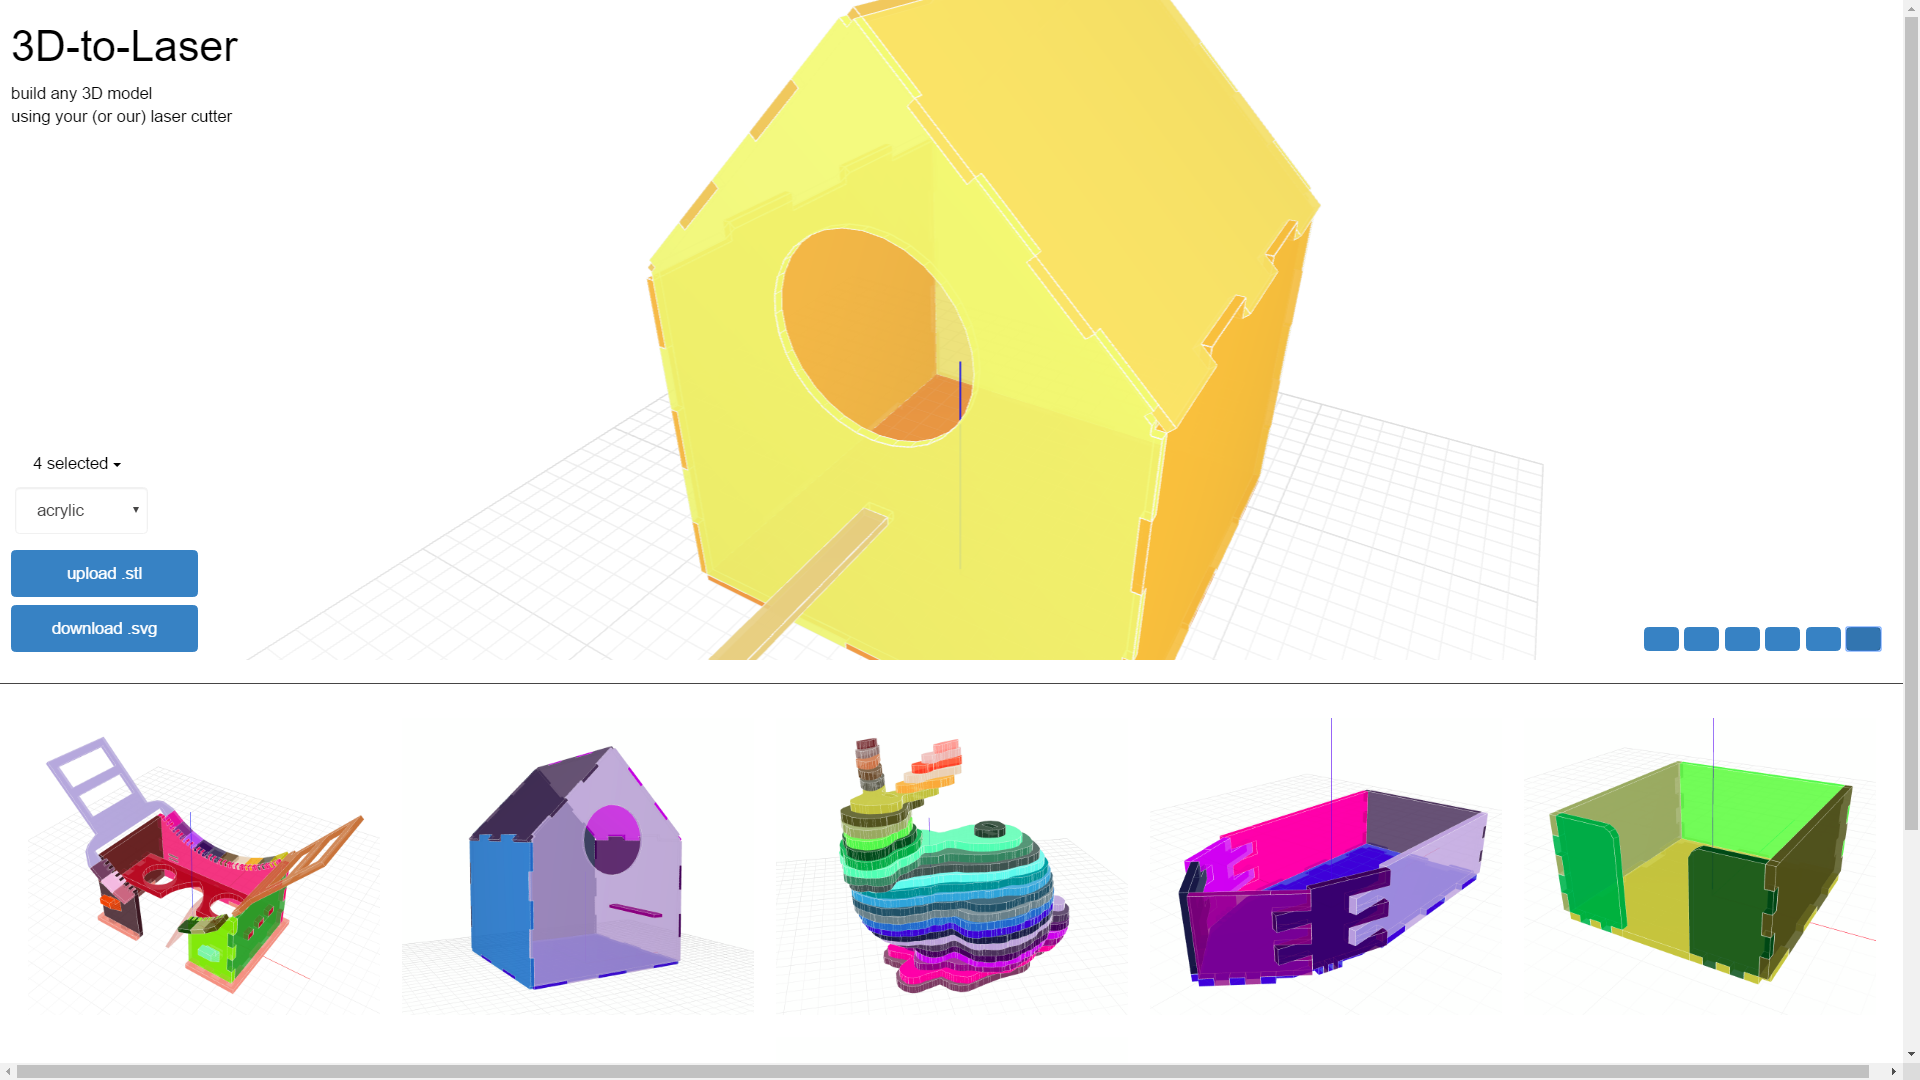
\includegraphics[width=1\columnwidth]{02-landing_page}
  \caption{The landing page with the conversion and the repository area.}
  \label{fig:landing_page}
\end{figure}

\subsection{The Conversion and Preview Area Provides the Main Functionality}

The conversion and preview area shows the currently selected or uploaded model. It also provides some conversion settings at the bottom left and visualization settings at the bottom right.

\subsubsection{Conversion Settings for Custom Material Selection}

To change which materials should be used for the conversion, the user can select multiple plate thicknesses in the top selection drop down (see Figure~\ref{fig:thickness_select}).

\note{To Do}

\subsection{The Repository Guarantees Fast Access to Lasercut-able Models}

\note{To Do}

\section{Customize View}

\subsection{Material Parameters}
\subsection{Device Parameters (Calibration)}

\section{Debug View}

\subsection{Pipeline Visualizations}
\subsection{Algorithm/ Method Selection}
\subsection{Testables (Operating Mode)}
\subsection{Console Debug Output}

\section{{\platener} as a Command Line Interface for Advanced Users}
\label{sec:walkthrough-cli}

We have seen in the preceding sections, how {\platener} is used in a
web browser.
% We intent to maximize scalability and user-friendliness
% by providing a web application.
Though converting a {\threedmodel} can be realized in a mere
drag-and-drop action using a web browser, we are limited to a single
conversion at a time. The web solution focuses on the results of the
conversion. Developers require a tool, that reports about the
conversion status and internal successful or failed processes. Our
software {\platener} provides a command line interface (CLI), which is
used in a terminal window. The CLI exposes commands for converting
{\threedmodel}s, processing multiple models in sequence and logging
progress reports. We explain the usage of the CLI in
Section~\sectionref{sec:walkthrough-cli-usage} and we demonstrate the logging
capabilities in Section~\sectionref{sec:walkthrough-cli-reports}.

\subsection{Usage Instructions of {\platener}'s CLI}
\label{sec:walkthrough-cli-usage}

A CLI is self-documenting. Listing~\ref{lst:cli-help} shows the
available commands.

\begin{listing}[!h]
\begin{minted}[
linenos
]{text}
node platener-cli.js -h

Specify an output directory.

  Usage: platener-cli [options] <output-dir>

  Options:

    -h, --help                output usage information
    -V, --version             output the version number
    -p --convertPath <input>  Convert multiple stl-Models to plates.
                              Give path to an folder with stl-Files.
    -f --convertFile <input>  Convert an stl-Model to plates.
                              Give path to an stl-File.
    -v --verbose              Enable Verbose Logging
    -s --subReports           Log Reports for each Fabrication Method
    --maxFilesize <input>     Limit filesize (MB),
                              so large files are skipped.

Full Help:

-f --convertFile    Generate all conversions for each
                    fabrication mode for the given stl-Model.
                    Each solution is stored in a seperate zip-File.
                    The zip-Files are written to the output directory.
\end{minted}
\caption{The help of {\platener}'s CLI.}
\label{lst:cli-help}
\end{listing}


The command line interface mirrors all the computational behavior of
{\platener} as a web application. With the CLI, we can convert a
single {\threedmodel} by loading data from the file system. The
conversion result is again a {\zipfile}. It is written to a given
target directory. We can recursively read input directories to
convert each {\stlfile} for the laser cutter. Both commands are given
in Listing~\ref{lst:cli-convert}.


\begin{listing}[!h]
\begin{minted}[
linenos
]{shell}
# convert a single file
node platener-cli.js -f ./stl/cubeFilled5cm.stl ./conversions

# convert an input directory
node platener-cli.js -f ./stl ./conversions
\end{minted}
\caption{Converting an {\stlfile} with {\platener}'s CLI.}
\label{lst:cli-convert}
\end{listing}

We can use the \emph{--maxFilesize} filter, to limit the
input files by their size in megabytes.

\subsection{Tracking Down Errors with Conversion Reports}
\label{sec:walkthrough-cli-reports}

Using the web application we either receive a successfully converted
{\svgfile} or the conversion fails. As the web interface is a
user-centered design we do not show extensive error messages or logs
of similar kind. For a developer it is crucial know where and under what
circumstances the software failed. With reports, we document the
conversion process. A report provides a short summary of the
conversion and gathers all error messages along the way, so a
developer can track down the issue. Figure~\ref{fig:report-simple}
shows a summary report. A report itemizing the results of our three
conversion approaches can be seen in Figure~\ref{fig:report-methods}.
In Figure~\ref{fig:report-error} an error message is depicted. When
multiple conversions were enqueued by {\platener}, we receive each
conversion report when the process finishes, as shown in
Figure~\ref{fig:report-multiple}.

\begin{figure}
  \centering
  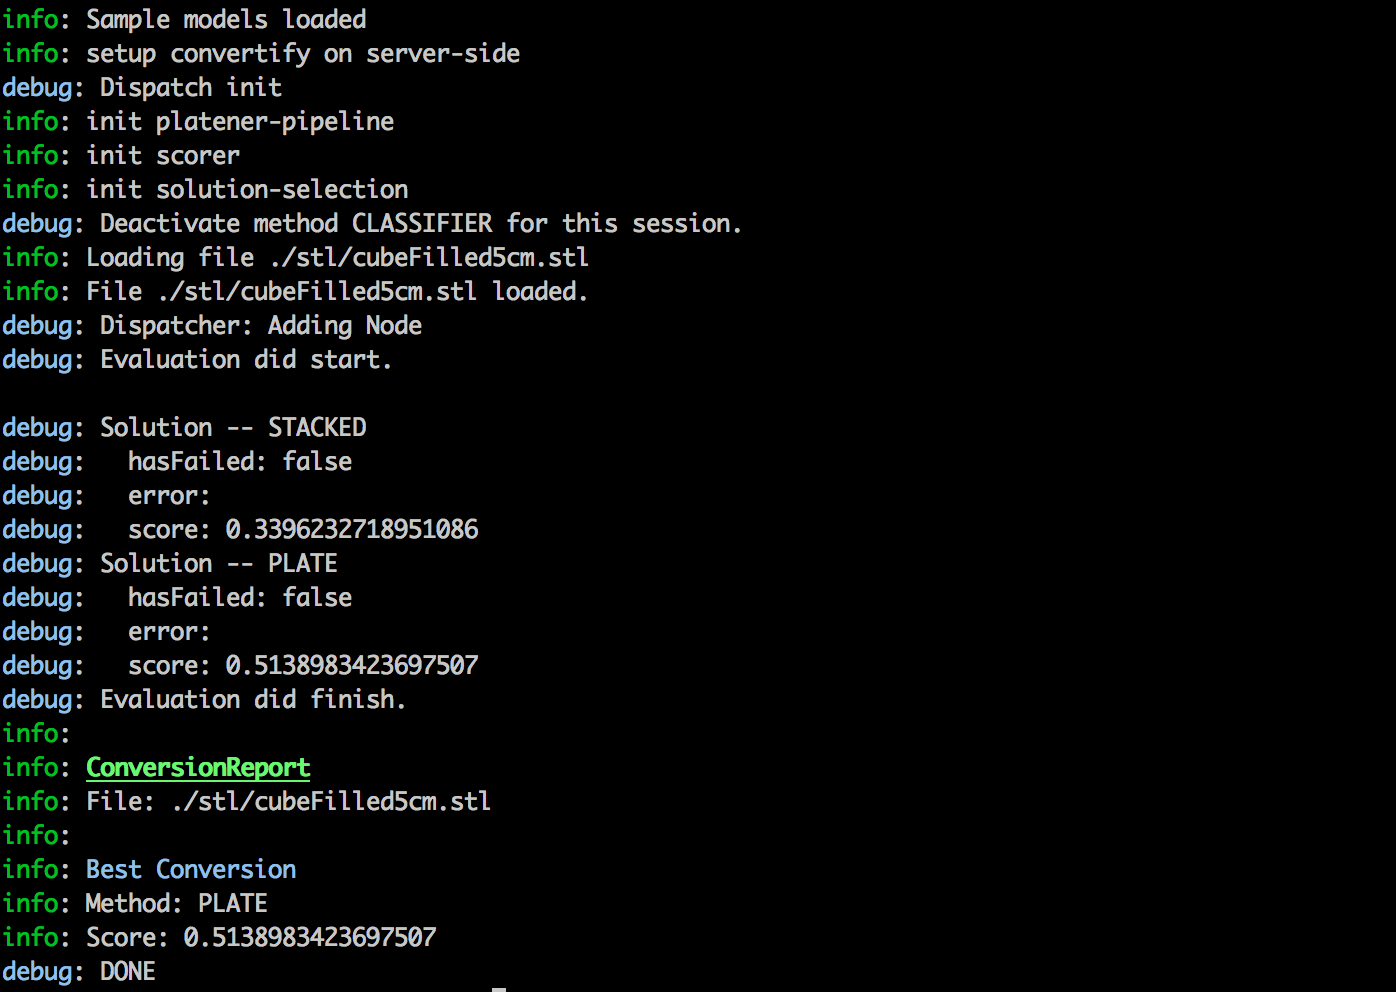
\includegraphics[width=1\columnwidth]{02-user-interaction-report-simple}
  \caption{A \class{Report}, showing a summary of the conversion.}
  \label{fig:report-simple}
\end{figure}

\begin{figure}
  \centering
  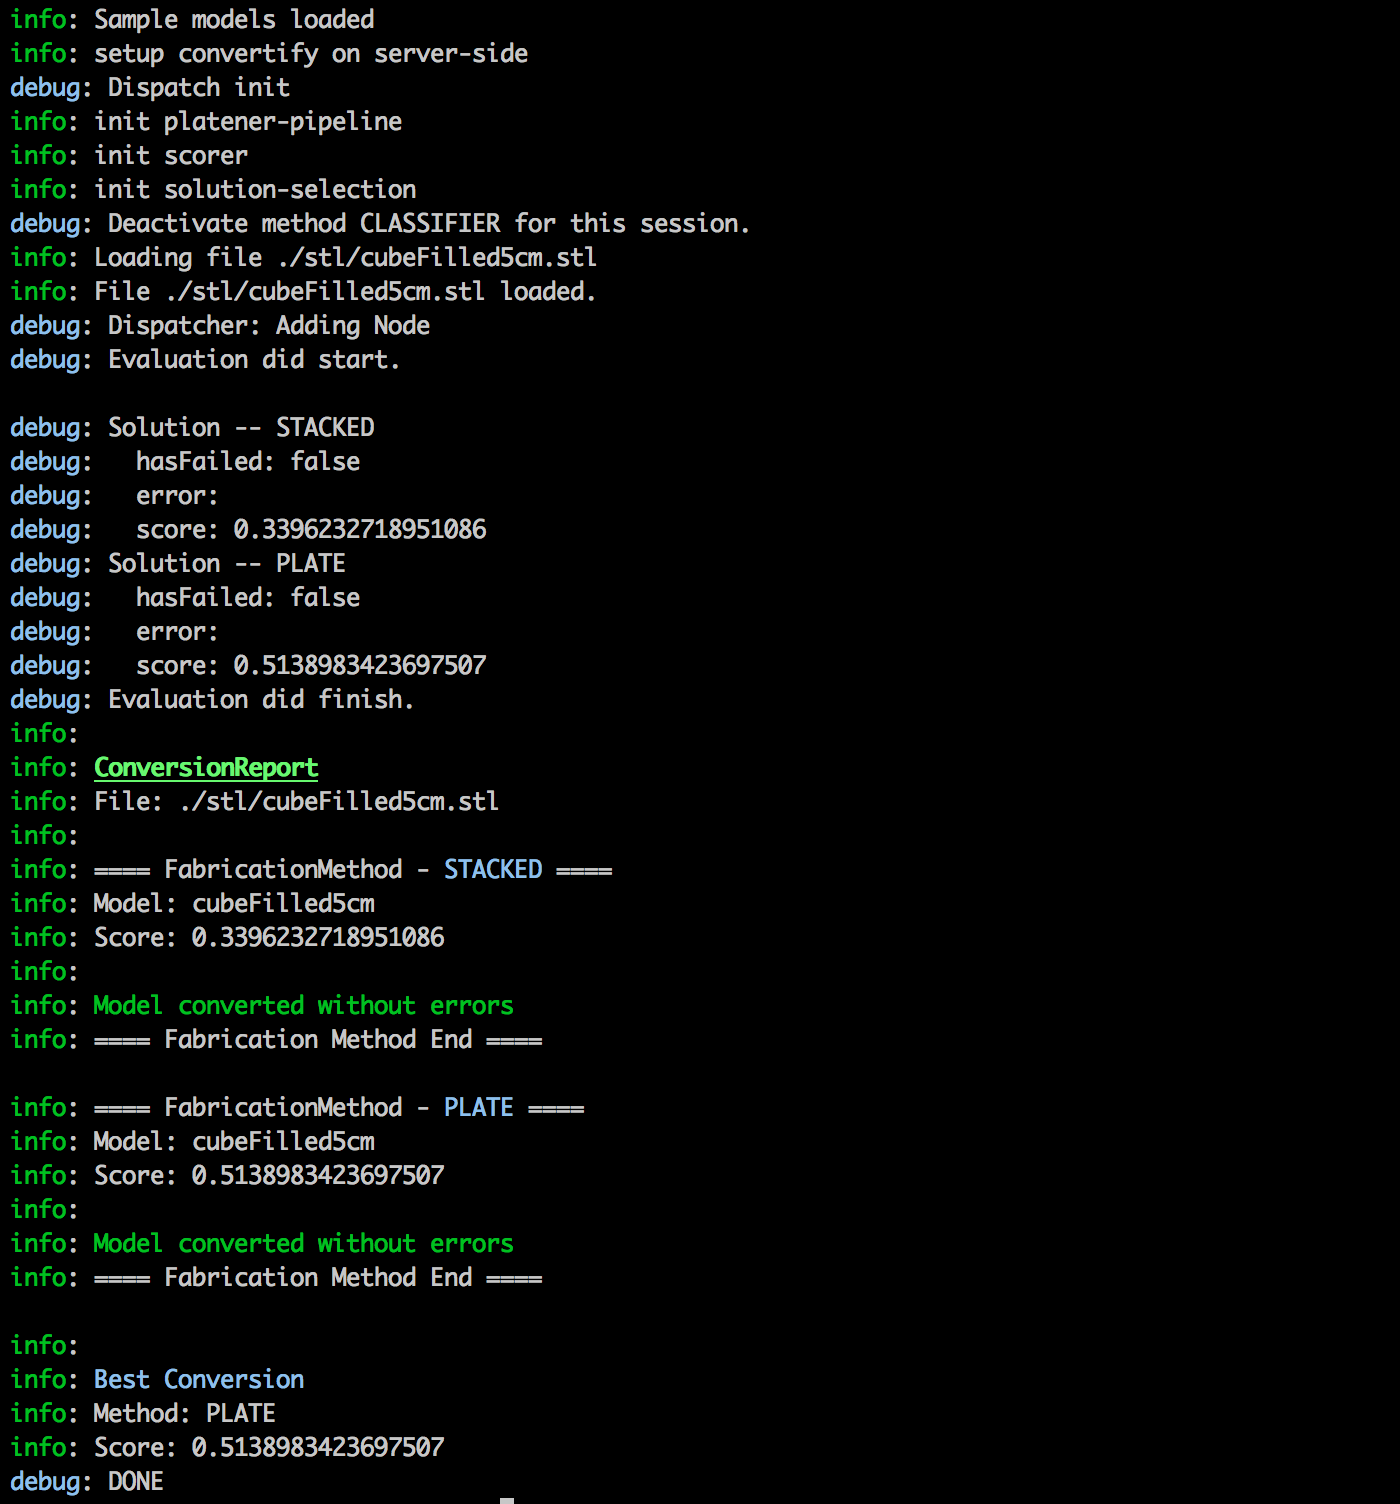
\includegraphics[width=1\columnwidth]{02-user-interaction-report-methods}
  \caption{A \class{Report}, showing a separate summary for each
    fabrication method of the conversion.}
  \label{fig:report-methods}
\end{figure}

\begin{figure}
  \centering
  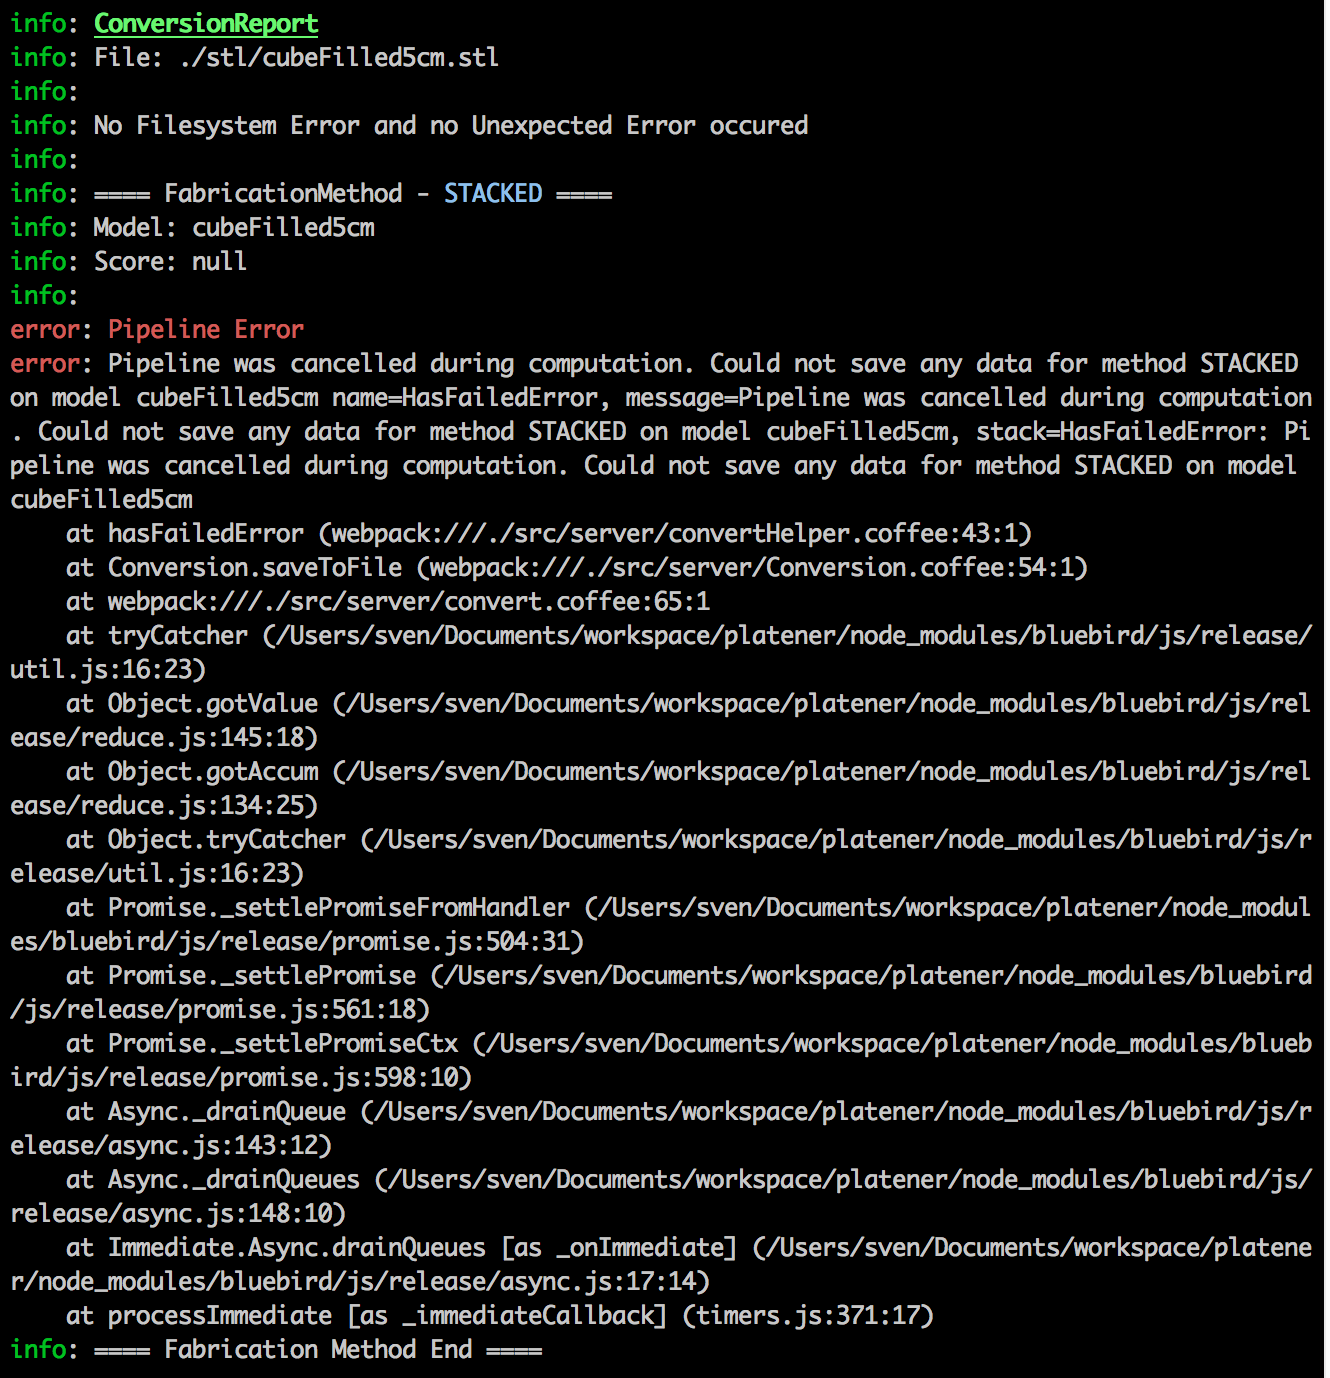
\includegraphics[width=0.8\columnwidth]{02-user-interaction-report-error}
  \caption{When a conversion fails the \class{Report} shows the error
    message.}
  \label{fig:report-error}
\end{figure}

\begin{figure}
  \centering
  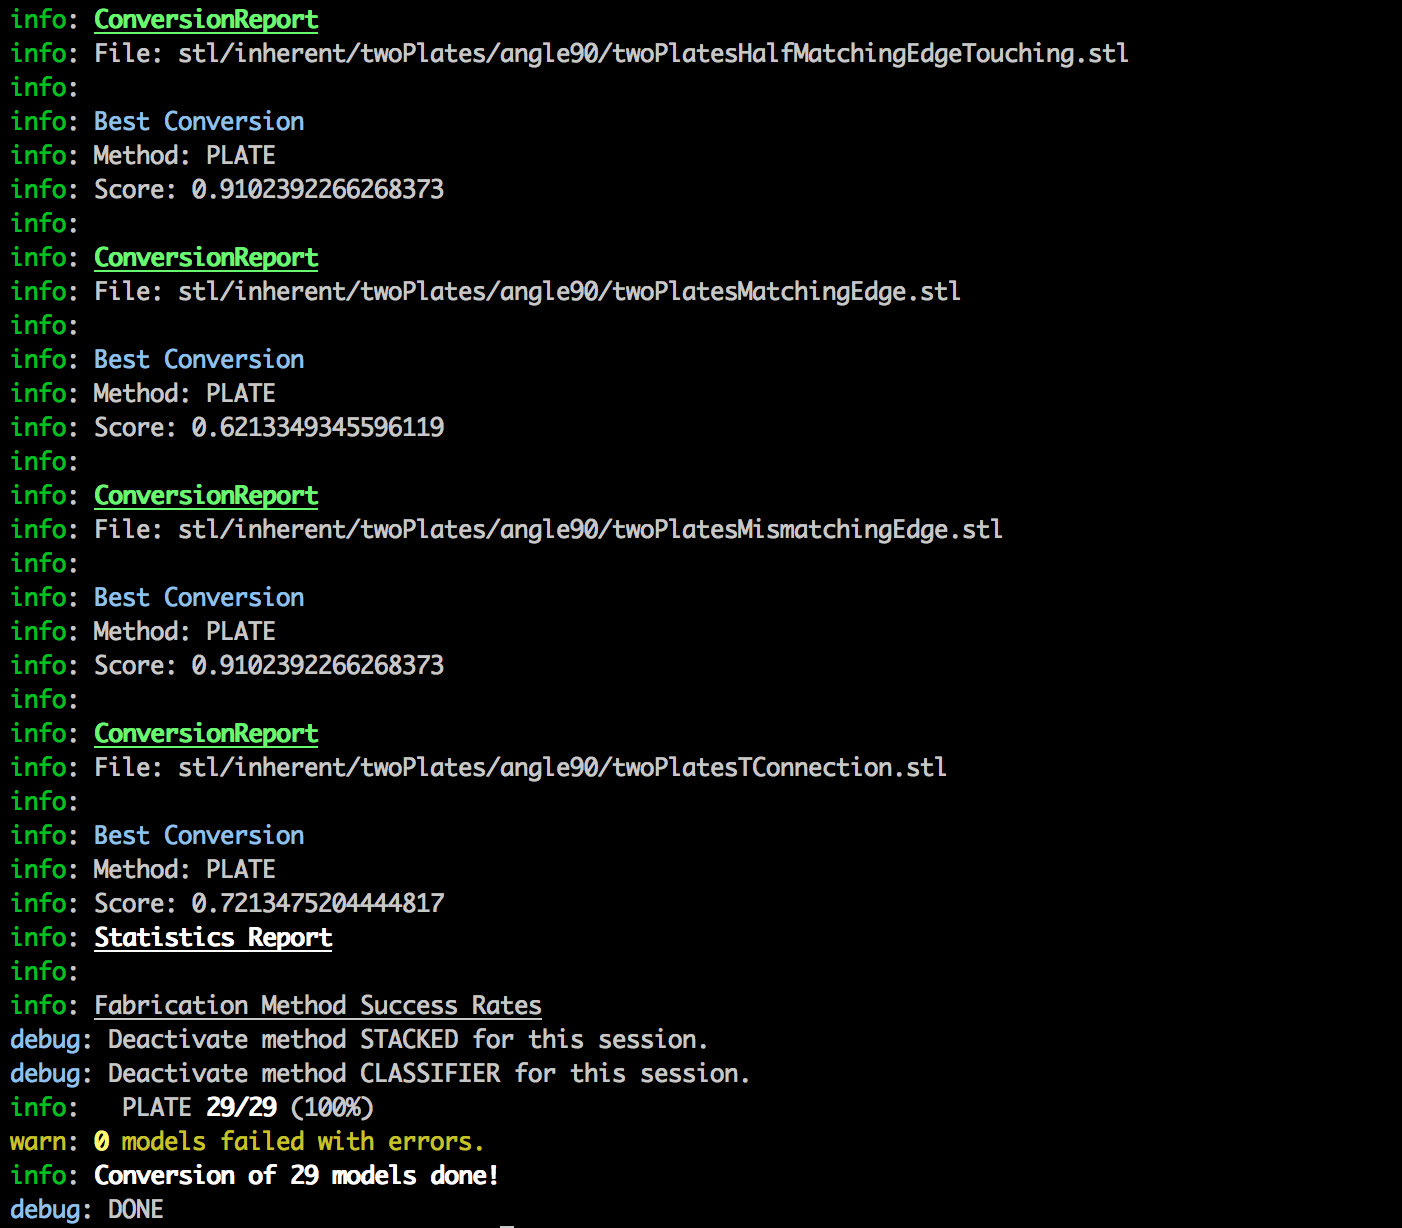
\includegraphics[width=0.8\columnwidth]{02-user-interaction-report-multiple}
  \caption{A sequence of conversions is summarized when the
    computation completed.}
  \label{fig:report-multiple}
\end{figure}



\end{document}

%%% Local Variables:
%%% mode: latex
%%% TeX-master: "../ClassicThesis"
%%% TeX-command-extra-options: "-shell-escape"
%%% End:

\cleardoublepage

%\part{Architecture}
% Sven
\subfile{Chapters/03-Architecture}
%\documentclass[../ClassicThesis.tex]{subfiles}
\begin{document}

\newcommand\myNotes[1]{\textcolor{red}{#1}}
\newcommand{\class}[1]{\emph{#1}}

% put this into the intro
% \platener is a web application,
% converts input {\threedmodels} into {\svgfiles}

% ************************************************
\chapter{Architecture}
\label{ch:architecture}
% ************************************************

In this chapter we outline the architecture and composition of the
application {\platener}. Therefore, we look at concepts of graphics
programming in web-environments in Section~\ref{sec:cg-web}. Then, we
explore the structure of our software from two points of view. At
first, we present {\convertify} in
Section~\ref{sec:framework-convertify}. {\convertify} is the
web-framework in which {\platener} is implemented. Secondly, we
explain the details of {\platener} in
Section~\ref{sec:application-platener}.\\
\\
With a framework like {\convertify} we can implement generic
{\threedmodel} manipulation web-applications. {\threedmodel}
manipulation means restructuring the model geometry in such a way,
that it can be used in a new context - apart from visualization on
computer screens. Such manipulations include converting the
{\threedmodel} for physical output devices like {\threedprinter}s or
{\lasercutter}s. For example, {\brickify} creates models consisting of
3D-printed parts and
{\lego}-assembled\footnote{\url{http://www.lego.com}} parts. Thus,
{\brickify} could ideally be built with {\convertify}.\\
\\
{\platener} is an application implemented in the framework {\convertify}.
Using a framework helps us focusing on the algorithmic challenges of
converting arbitrary {\threedmodel}s into physical, laser-cut output.

\section{Computer Graphics in Web-Environments}
\label{sec:cg-web}
% ************************************************

In this section we give a brief overview of graphics programming
fundamentals in general and in web-environments. These fundamentals
are the concepts of {\threedmodel} data representation in
Section~\ref{sub:model-representation} and render loops and scene
graphs in Section~\ref{sub:render-and-graph}.

\subsection{{\threedmodel} Representation}
\label{sub:model-representation}

This section explains which data structures and disk-formats are used
to represent {\threedmodel}s. First, we explain the terminology of
meshes. Secondly, we look at the {\stlfile} format\\
\\
The model geometry is represented by a set of connected polygons,
approximating the model surface. These connected polygons form a mesh.
Figure~\ref{} shows a mesh. For the sake of simplicity, we use
triangles as polygons. A triangle in the mesh is called face. Each
face is described by a list of three coordinates in 3D-space. Such a
coordinate is called vertex \cite[p.~3]{cg-intro}. An edge is the line
between two connected vertices.\\
\\
We only support geometry which is arranged in two-manifold meshes.
Two-manifoldness is a constraint on the mesh, which requires each egde
to only touch two neighboring faces. Figure~\ref{}\myNotes{add figure}
shows a comparison of a manifold and non-manifold part of a mesh. It
follows then, that each triangular face has to have three adjacent
faces. Thus, the constraint enforces the mesh to be a fully connected
graph without holes \cite[p.~28]{master-thesis}. We require
two-manifoldness to make
sophisticated assumption when designing the conversion algorithms.\\
\\
The Standard Tessellation Language (STL) format is a common file
format for {\threedmodel} representation in the context of
{\threedprinting}. We support the {\stlfile} format, because our goal
is to make models, built for a {\threedprinter}, available for the
{\lasercutter}. An {\stlfile} consists of a list of faces associated
with their face normal. The face normal determines the orientation of
the face. We need the face normal, because from the vertices only, we
cannot say in which direction the face points. Each face is a list of
vertices. A vertex is described by three floating point numbers.
Listing~\ref{alg:stl-file} shows an {\stlfile} in ASCII encoding. For
saving disk-space, the file is mostly stored in a binary format
\cite[p.~8]{stl-file}.

% \begin{algorithm}
%   \caption{General format of a STL-file in ASCII encoding.}
%   \label{alg:stl-file}
%   \algblock[Name]{solid}{endsolid}
%   \begin{algorithmic}
%     \solid \textit{name}\\
%     facet normal \textit{n1} \textit{n2} \textit{n3}\\
%       outer loop\\
%        vertex \textit{p1x} \textit{p1y} \textit{p1z}\\
%        vertex \textit{p2x} \textit{p2y} \textit{p2z}\\
%        vertex \textit{p3x} \textit{p3y} \textit{p3z}\\
%       endloop\\
%      endfacet\\
%     \endsolid \textit{name}
%   \end{algorithmic}
% \end{algorithm}

Reconstructing the original {\threedmodel} from an {\stlfile} does not
always result in one-to-one solution. The vertices are stored with
floating point numbers instead of referring to the same vertex with an
index. Thus, we have to assume, that two overlapping points represent
an identical vertex. We use the library {\meshlib} to create an
indexed face-vertex-mesh from the possibly ambiguous {\stlfile}. With
{\meshlib} we can convert the face-vertex-mesh representation to a
{\threejs} geometry. With a {\threejs} geometry, we can render a
{\threedmodel} in {\convertify}.\\
\\
To support a variety of {\threedprinter} optimized models, we use the
{\stlfile} format. We import the files with the {\meshlib} library.
The imported face-vertex-mesh structure is then converted for usage
with {\threejs}. The section below, explains how the {\threejs}
representation is displayed on the screen.

\subsection{Render Loop and Scene Graphs}
\label{sub:render-and-graph}

To understand how {\convertify} and {\platener} work, we have to
familiarize with the concepts of rendering and scene graphs first. \\
\\
A typical pattern any graphics software cannot live without is the
render loop. Rendering is the process of turning the {\threedmodel}
representation into an array of pixels which can be displayed on the
screen~\cite[p.~2]{intro-cg}. The render loop pattern consists of
three steps: processing input, updating the {\threedmodel}
representation and rendering~\cite{gamedev-gameloop}.
Figure~\ref{fig:render-loop} shows an exemplary flow.\\

\begin{figure}[h]
  \centering
  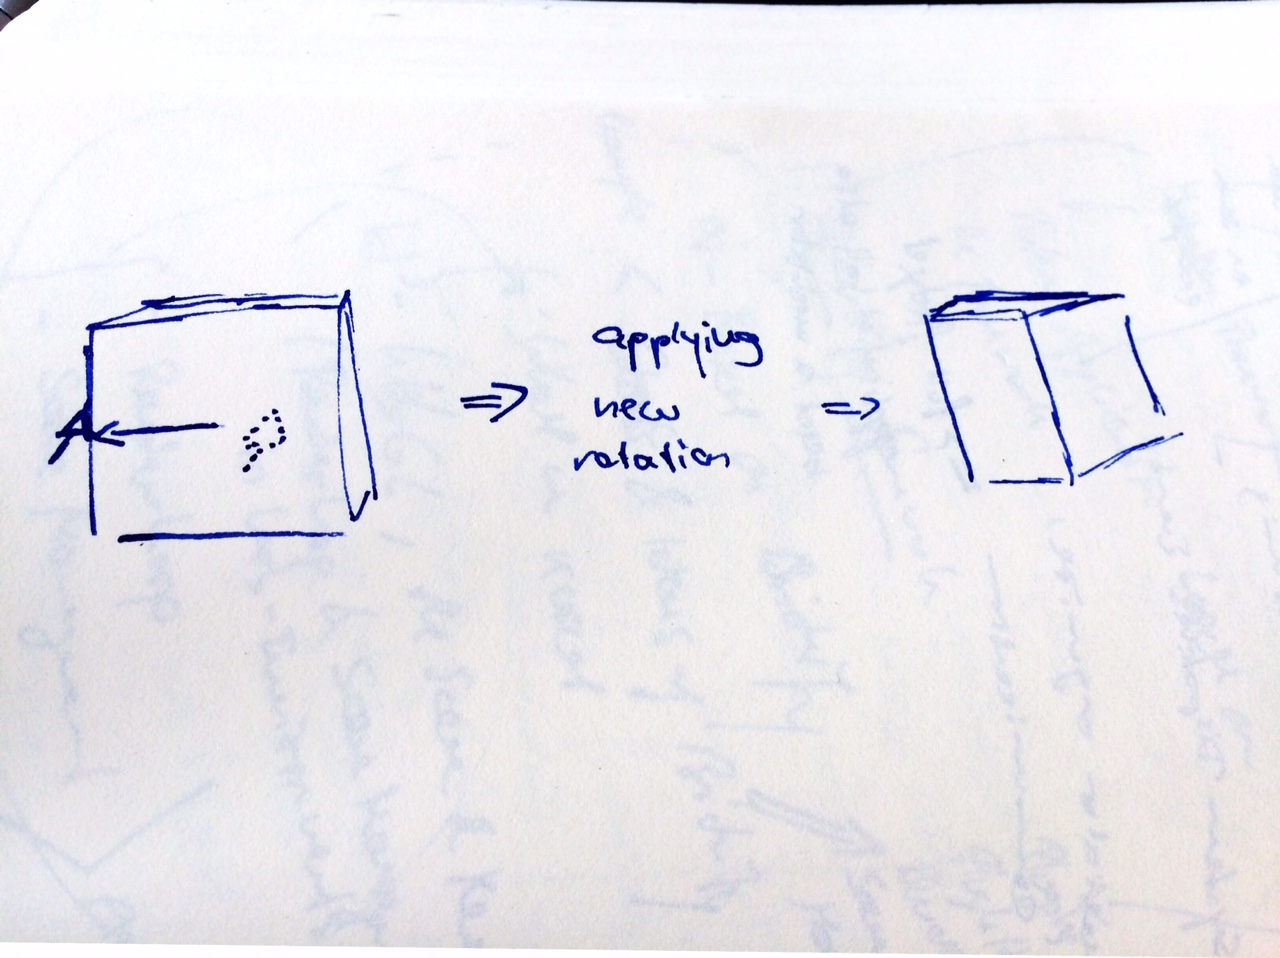
\includegraphics[width=1\columnwidth]{03-architecture-render-loop}
  \caption{Touch input is processed by the render loop.}
  \label{fig:render-loop}
\end{figure}

When an object is rendered on the screen, it is part of a scene. A
scene is the visual space, in which the rendered objects can be seen.
Instead of rendering each vertex of the model directly to the scene,
we use representations of objects, which are organized in a
hierarchical data structure. We refer to this hierarchical structure
as scene graph. A simple scene graph is depicted in Figure~\ref{}. The
shown graph contains a box as single root node. The sides of the box
are children of the root node. With this abstraction we can easily
apply transformations to parts of the model only, without necessarily
touching each face or vertex. Every object, that is rendered by
{\convertify} is part of a scene graph.

\begin{figure}[H]
  \centering
  \begin{subfigure}[b]{0.49\textwidth}
    \centering
    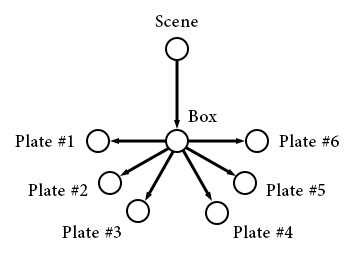
\includegraphics[width=\textwidth]{03-architecture-scene-graph-abstract}
    \caption{Graph notation of the composed box.}
    \label{fig:scene-graph:abstract}
  \end{subfigure}
  \begin{subfigure}[b]{0.49\textwidth}
    \centering
    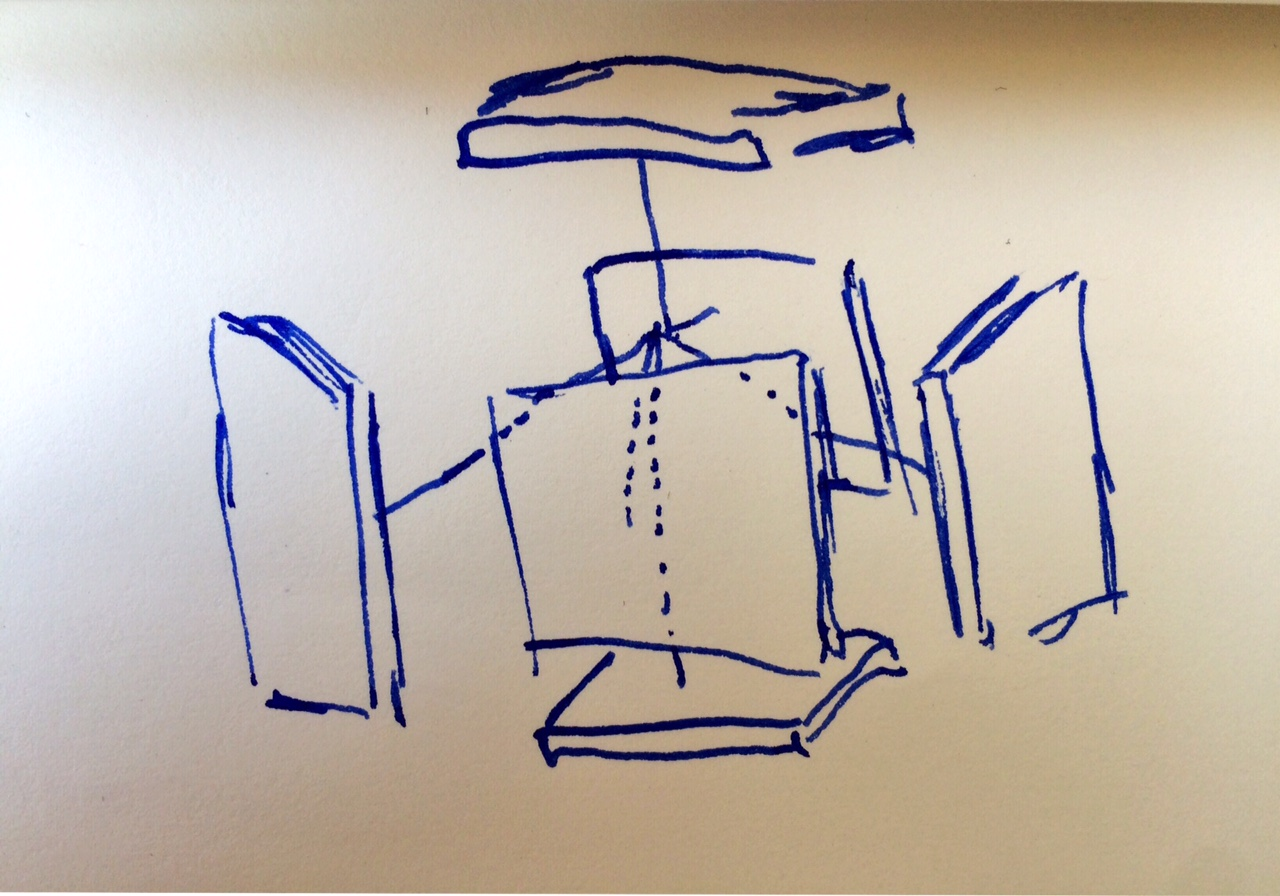
\includegraphics[width=1\textwidth]{03-architecture-scene-graph-visual}
    \caption{Rendered box, showing decomposition into plates.}
    \label{fig:scene-graph:visual}
  \end{subfigure}
  \caption{A scene graph showing a box, composed of plates.}
  \label{fig:scene-graph}
\end{figure}

To enable full-fledged rendering results with sophisticated visual
effects in web-browsers, we have to use the Web Graphics Library
(WebGL). With the use of WebGL we can process data on the GPU and
execute special effects code (shader code)~\cite{mdn-webgl}.
\\
On top of WebGL we use {\threejs}\footnote{\url{http://threejs.org}}.
{\threejs} is a {\javascript} library, which wraps the WebGL API and
attempts to make the usage of WebGL simpler. It provides a scene graph
implementation. {\threejs}
data representations are used throughout {\convertify}.\\
\\
The framework {\convertify} uses common computer graphics patterns
like render loops and scene graphs. With the help of WebGL and
{\threejs} we are able to bring these concepts into a web-environment.

\section{The Framework: Convertify}
\label{sec:framework-convertify}

In this section we present {\convertify}, a web-framework for working
with {\threedmodel}s in {\threejs}. The framework is based on
previous work by \citeauthor{brickify-thesis}. We explain the work and
concepts of \citeauthor{brickify-thesis} in
Section~\ref{sec:based-brickify}. Then we outline, how we incorporated
the previous work into {\convertify} in
Section~\ref{sec:reuses-brickify} and Section~\ref{sec:plugin-system}.

\subsection{The Framework is Based on Brickify}
\label{sec:based-brickify}

The framework {\convertify} is based on the application {\brickify} by
\citeauthor{brickify-thesis}. {\brickify} is a web-application which
converts {\threedmodel}s into a hybrid model, consisting of {\lego}
bricks and fewer 3D-printable parts. The previous work provides
features like rendering or scene graphs, which can be shared with
{\convertify}. In this section we present important design decisions
of {\brickify}, which will help understanding how our framework
works.\\
\\
{\brickify} implements a flat scene graph using \class{Nodes}. Each
\class{Node} references an input model, has a {\threejs} object and
transforms. The {\threejs} object is a \class{THREE.Object3D}. This is
a generic object, which can be rendered into a WebGL scene with
{\threejs}. This \class{THREE.Object3D} will be displayed on the
screen by {\brickify}. The transforms describe spatial properties like
position, scale or rotation and are applied to the {\threejs} node.
Note, that \class{Nodes} represent entities in the scene, but only
{\threejs} nodes can actually be rendered.

The \class{Nodes} are part of a \class{Scene}. The \class{Renderer}
sets up a WebGL context and initializes {\threejs}. Then the
\class{SceneManager} passes all active \class{Scenes} to the
\class{Renderer}, which will traverse the flat scene graph and render
each attached \class{THREE.Object3D}. Figure~\ref{}\myNotes{add
  figure} shows how these classes interact. During that loading and
render process, {\brickify} emits system events, e.g. change events to
the scene graph (\textit{onNodeAdd},
\textit{onNodeRemove}).\\
\\
{\brickify} decomposes its features into \class{Plugins}. A
\class{Plugin} provides a set of methods which can be called upon
system events to interact with the WebGL scene.
\citeauthor{brickify-thesis} refers to these callbacks as
\class{PluginHooks} or just hooks.

User interfaces are implemented in a separated code package. This
mostly separates the web-interface from the scene features. The
interface code uses a \class{Bundle} as an entry point to the plugin
and scene system. The \class{Bundle} starts \class{Plugins} and loads
{\threedmodels} from the filesystem into the application.\\
\\
{\brickify} provides abstractions for scene management and rendering.
Plugins interact with the internal system via hooks. The separation of
{\lego}-conversion features from the rendering engine bring clear
interfaces. We encountered several hick-ups with this architecture
when we tried to organize the communication between several plugins.
In the following section, we outline our improvements to the internal
system of {\brickify}.

\subsection{The Framework Reuses Ideas and Components of Brickify}
\label{sec:reuses-brickify}

\subsection{The Framework Provides an Enhanced Plugin System}
\label{sec:plugin-system}



\section{The Application: Platener}
\label{sec:application-platener}



















\section{Architecture Overview}
% ************************************************

\begin{figure}
  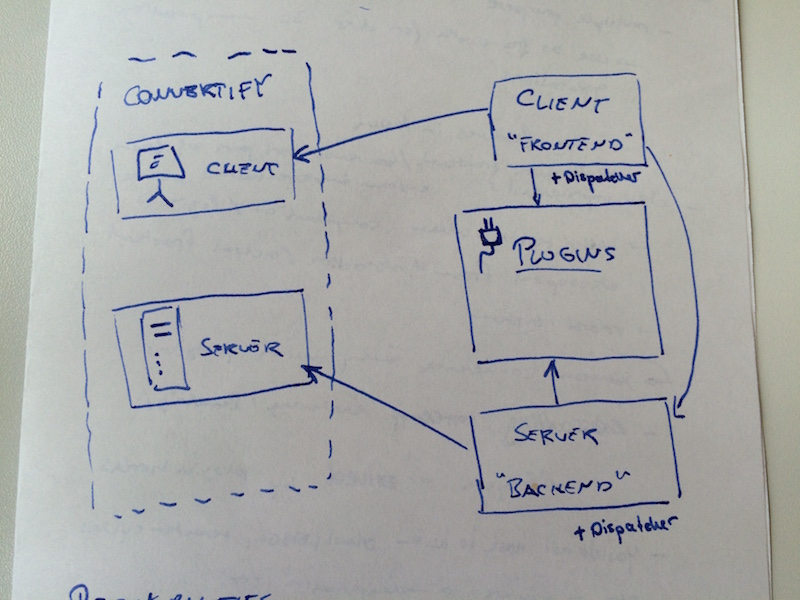
\includegraphics[width=1\columnwidth]{03-architecture_overview_current}
  \caption{Main Packages of the Platener Architecture}
  \label{fig:architectureOverviewCurrent}
\end{figure}

Platener is designed to enable web-based manipulation and rendering of
{\threedmodel}s. Figure \ref{fig:architectureOverviewCurrent} shows the major
packages \emph{Convertify}, \emph{Client}, \emph{Server} and \emph{Plugins}. The
arrows indicate dependencies between the packages. The architecture emphasizes a
uni-directional data and event flow. Similar to mobile application design,
lifecycle events and the concept of
delegation\footnote{\url{https://developer.apple.com/library/ios/documentation/General/Conceptual/DevPedia-CocoaCore/Delegation.html}}
establish clear communication among packages.

% \begin{itemize}
% \item platener built on top of...
% \item 4 major packages: convertify, client, server and plugins
% \item optimized towards: working with 3d-models in webgl environment
% \item plugin-based: allow interchangeable computation logic/ conversion methods
% \item combination of lifecycle-based communication and explicit calls via
%   dispatchers (related work: mobile application design, mediator pattern) \ritem
%   explicit communication between packages
% \end{itemize}

\subsection{Package Responsibilities}

Each package takes over a set of distinct responsibilities ensuring decoupled
components. Thus a flexible, maintainable system is created.

\emph{Convertify} provides generic tools which support plugins in manipulating
{\threedmodel}s. This includes utilities for vector analysis as well as
rendering routines and scene management. The application lifecycle can be
initiated and observed via a \emph{Bundle}. A Bundle represents an instance of
the application's computation unit. The Client and Server packages run a Bundle.

\emph{Plugins} provide an exchangeable set of features which are used by the
Client and Server package. A Plugin interacts with the Scene and its
{\threedmodel}s via lifecycle events. E.g. a concrete conversion strategy
provided by Platener is implemented by a single Plugin. Plugin features can be
enabled for Client, Server or both.

The \emph{Client} package gives the look and feel of the application. This
package contains frontend components. The developer can choose any template
engine\footnote{\url{http://www.sitepoint.com/overview-javascript-templating-engines/}}
which serves the application's purpose. So the Client wires up the
{\userinterface} and the computation logic.

The \emph{Server} package is the headless\footnote{A headless web-application
  runs without the graphical user interface of browsers.} counterpart to the
Client package. A Command Line Interface enables the user to run the application
without a browser. The Server also satisfies requests from the Client, such as
caching and loading models in a RESTful
interaction\footnote{\url{http://www.drdobbs.com/web-development/restful-web-services-a-tutorial/240169069}}.

% \begin{itemize}
% \item convertify: generic tools, helpers for 3d rendering, scene management,
%   model manipulation, platener independent
% \item client: look and feel, ux user interactions, wiring up/ firing up
%   computations, implemented for platener
% \item server: model storage/ cache, REST interaction, headless version of
%   client, CLI-tool chain, implemented for platener
% \item plugins: conversion specific computation and logic units, addons for
%   frontend and backend, platener independent
% \end{itemize}


\subsection{Decoupling the Software into Packages}

Decoupling the software into packages builds a robust system. Computation logic
and UX components are kept apart, which allows isolated testing.

\subsubsection{Convertify Is a Framework}

The \emph{Convertify} package is meant to be used as a white-box framework for building
3D manipulation applications. Platener is such an application, supporting model
imports, rendering, altering and export of geometries. Introducing a web
framework makes sense, because WebGL gets more and more stable as of the year
2016 \myNotes{TODO: reference!}. Thus graphics software can be brought to huge
audience providing cross-platform web services. For example \emph{Brickify} or \emph{Laser
Origami}\myNotes{ref} could be implemented with \emph{Convertify}.

% \begin{itemize}
% \item multpiple purpose:
% \item use as (whitebox) framework for other 3D manipulation applications (related work:
%   mechanism mining, etc)
% \item web service --> highly available, cross platform
% \item plug features in and out
% \item because concrete frontend/ backend not part of framework, custom
%   implementations possible (no vendor lock) \myNotes{this should be part of the
%     comparison with Brickify}
% \end{itemize}

\subsubsection{Plugins Establish Focus on Graphic Problems}

Plugins are self-contained units which mainly interact with the WebGL scene and
its scene graph. Whole feature-sets can be switched on or off at once. They are
loosely coupled but have high cohesion at the same time. This prevents spaghetti
code and supports maintainability of each component. Furthermore, we use
software hooks to integrate plugins with rendering of models and access to
geometry data. This event-based approach enables developers to write a 3D
manipulation tool without having detailed domain knowledge about WebGL and
web-services. This allows developers from the Computer Graphics domain to
concentrate on the graphics problem, rather than the web-environment.

% \begin{itemize}
% \item dev improvements:
% \item better testing of computation/ logic because decoupled from ux
% \item robust system
% \item --> loose coupling of plugins, high cohesion in plugins
% \item --> isolated testing/ development possible
% \item solve cross-cuts: rendering/ loading <> lifecycle of plugins (eventbased)
% \item you do not have to know about WEBGL, render cycles etc. to provide a 3D
%   manipulation tool
% \item --> minimize web-domain knowledge as CG-devs are often unfamiliar with
%   this environment
% \end{itemize}

% \subsection{Discussion "vs Brickify"}

\subsubsection{A Comparison with the Brickify Packages}
\myNotes{maybe put statement, rather then description into headline}

The Convertify package is not present in the Brickify architecture, see Figure
\ref{fig:architecture_overview_brickify}. This means Brickify provides a mix of
UX components, computation logic and interfacing code in the Client and Server
packages. Plugin communication is hard to observe and only implicitly ordered.
We introduce the new package to escape the vendor lock\myNotes{explain vendor
  lock} of previously used UX libraries. Libraries like \myNotes{add refs}
\emph{jQuery} and \emph{Jade} \myNotes{now pug} scatter code throughout the
project. By removing UX dependencies from logic components we create a
thoroughly testable code base.

\begin{figure}
  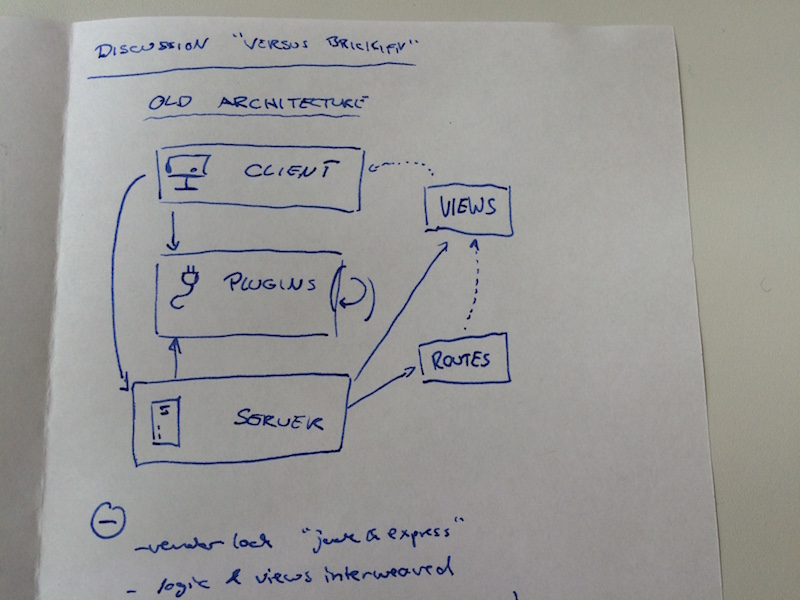
\includegraphics[width=1\columnwidth]{03-architecture_overview_brickify}
  \caption{Main Packages of the former Brickify Architecture}
  \label{fig:architecture_overview_brickify}
\end{figure}

% \textbf{pros}
% \begin{itemize}
% \item fast enhancements as only views/ routes have to be adapted
% \item less interfacing because frontend <> logic tightly coupled
% \end{itemize}
% \textbf{cons}
% \begin{itemize}
% \item vendor lock: jade and express
% \item logic and views interweaved: high coupling --> hard testing, hard
%   maintainability, hard to change things
% \item implicit plugin communication
% \item complex management of custom 3d manipulation tools would require a lot of
%   rewrites because of view/ logic mix
% \end{itemize}

\section{Convertify Package and its Plugin Architecture}
% ************************************************

Platener uses the Convertify package as entry points to the {\threedmodel}
processing. The package provides features for browser- and
headless-environments.

It encapsulates basic logic for {\threedmodel} manipulation and model import.
Additionally, we provide utilities to simplify working with \emph{\threejs} or
rendering objects into scene.

Convertify handles the scenegraph of the application. \emph{Nodes} are injected
into the scene \myNotes{ref brickify} and lifecycle events are emitted, e.g. on
load, on draw or on touch interactions with the \emph{Node}.

% \begin{itemize}
% \item entry points
% \item headless startup
% \item basic logic for 3dmodel manipulation (import, mesh-conversion)
% \item scenegraph and rendering (nodes, refs for sync objects in Brickify)
% \item plugin interaction (hooks)
% \item application helpers (threeHelper, renderHelper, commons (we should move
%   commons to convertify))
% \end{itemize}

\subsection{Scene Graph and Scene Management}

\myNotes{this is crap somehow}
The scene graph is built from \emph{Nodes}. Each \emph{Node} is associated
with a single \emph{THREE.Object3D} instance. This instance is rendered by the
WebGL renderer. The \emph{Node} is a high-level abstraction of objects in the
scene graph. \emph{THREE.Object3D} instances contain fine-grained sub-objects and
actual vertices. For each Plugin we provide further \emph{THREE.Object3D}
instances, which belong to the \emph{Node}'s \emph{THREE.Object3D}.

\emph{Nodes} belong to a \emph{Scene}. Multiple \emph{Scenes}
are added to a \emph{Project}. The \emph{Project} is the single root node of the
scene graph. \emph{Nodes} are added and removed by the \emph{SceneManager},
which is controlled in a \emph{Bundle}.

% For each \emph{Plugin} we provide further \emph{THREE.Object3D}
% instances, to which the \emph{Plugins} can append their computed visuals.

% \begin{itemize}
% \item project -> scene (one active, multiple hidden) -> node
% \item a single project per application
% \item manages a scene (shallow representation of actual WEBGL scene, high level
%   objects)
% \item node - object in the scene (represents arbitrary data loaded into scene,
%   has transforms)
% \item the model you see is a node
% \item rendering in Renderer (WebGL renderer abstraction)
% \item update loop, plugins may manipulate the model -> changes displayed
% \end{itemize}

\subsection{Lifecycle Events with Plugin Hooks}

\subsubsection{The Internal System Emits Lifecycle Events}

Similar to other applications\myNotes{what applications?} \emph{Convertify}
dispatches events from the internal system during the application's lifecycle.
The internal system refers to framework features, which all applications built
with \emph{Convertify} share. Such features are model import, scenegraph
manipulation or render updates.

\myNotes{add figure environment here}

The lifecycle of \emph{Convertify} is depicted in Figure \myNotes{add figure for
  platener lifecycle}. First we initialize all activated plugins in the
\emph{init} event. During the \emph{init3d} event each plugin is passed an empty
\emph{THREE.Object3D} instance. We call it the root node. The root node is
associated with the \emph{Node} in the scene graph. The plugins append
the computed visuals onto the root node. All root nodes are rendered by the
\emph{Renderer}, calling the \emph{update3d} callback. \myNotes{look up event
  name}. When a \emph{Node} from the \emph{Scene} is selected by the user, we
dispatch the \emph{onNodeSelect} event. When a new \emph{Node} is added to the
\emph{Scene}, the \emph{onNodeAdd} hook is triggered. The \emph{onNodeRemove}
hook is triggered respectively when a \emph{Node} is removed from the
\emph{Scene}. \myNotes{ref brickify}

% \begin{itemize}
% \item plugin init - plugin is loaded, general setup
% \item scene init -
% \item scene adding
% \item scene rendering/ update/ brushing
% \item scene selecting
% \item scene removing
% \end{itemize}

% \begin{itemize}
% \item App Lifecycle: Model Loading
% \item Plugin Init
% \item Scene Refreshes
% \item Scene Graph Interactions
% \item refer to Brickify
% \end{itemize}

\subsubsection{Plugins Interact with the Internal System via Lifecycle Events}

The subscribers to lifecycle events are \emph{Plugins}. Each event type exposes
a \emph{PluginHook}. Each \emph{Plugin} registers a callback on an arbitrary
number of events. These callbacks get called when the event is dispatched by the
system. Thus plugins can handle each event and apply their own functionality to
the scene or even the model geometry. With this we emphasize compact computation
units in plugins, which can still interact freely with the system. The approach
is directly adapted from \emph{Brickify} \myNotes{ref chapter in brickify}.

% \begin{itemize}
% \item Gain control for computation units (plugins)
% \item interact with the system
% \item plugin hooks (refer to pluginHooks.yaml)
% \item called on each plugin
% \item allow plugin to handle the event (e.g do some manipulation to the scene)
% \end{itemize}

\subsection{Plugins within Convertify}

A \emph{Plugin} bundles methods and system event callbacks to provide a new set
of features to the application, e.g. the \emph{PlatenerPipeline} plugin builds a
two-dimensional construction plan from the {\threedmodel} and exposes it for
download. The \emph{Plugin} can be switched on or off on application load for
the Client and Server package respectively. Complex applications can be built by
composing multiple plugins. This supports the framework character of
applications built with Convertify.


% \begin{itemize}
% \item part of the Plugin Package
% \item pluggable set of feature
% \item or self-contained unit
% \item can be activated for server/ client
% \item composing multiple plugins --> extensible, maintainable method of building
%   complex applications
% \end{itemize}


% \begin{itemize}
% \item Convertify as a framework
% \item do not mix logic/ ui
% \item decomposable logic (no spaghetti code)
% \end{itemize}


\subsubsection{Plugins Are Packages of Their Own}

Each \emph{Plugin} resides in the Plugin Package. We define a
\emph{package.json} file, which contains metadata of the package, see Listing
\ref{lst:packagejson}. Conceptionally, a \emph{Plugin} can be a separate
\emph{npm} package\footnote{Node Package Manager,
  \url{https://docs.npmjs.com/getting-started/what-is-npm}}. This means plugins
could be installed like any other typical dependency. For the sake of
development speed, we do not use the \emph{npm} setup yet. \myNotes{ref brickify}

\begin{listing}[ht]
\begin{minted}[
linenos
]{json}
{
  "name": "platener-pipeline",
  "version": "1.0.0",
  "description": "modifies model mesh to enable lasercuttable parts",
  "browser": "./PlatenerPipeline.coffee",
  "main": "./PlatenerPipeline.coffee"
}
\end{minted}
\caption{\emph{package.json} file of \emph{PlatenerPipeline} plugin.}
\label{lst:packagejson}
\end{listing}

To register a \emph{Plugin} with \emph{Convertify}, we have to add an entry in
the \emph{PluginMap}. The \emph{PluginMap} is a static dictionary, enumerating
all installed plugins and their filepaths. Because \emph{\nodejs} as well as
\emph{\essix} do not support dynamic require statements\footnote{A dynamic
  require statement can include and interpret source files into runtime where
  file paths are generated during runtime.}, we have to list each package
explicitly. In future systems we could alter the build system to include plugin
files automatically before compilation step.

The exposed main file of the package implements a set of \emph{PluginHooks}.
These hooks are registered at the \emph{Dispatcher}, which is responsible for
dispatching the lifecycle events to the plugins in a predefined order\myNotes{,
  see chapter ??}. Beside \emph{PluginHooks}, a \emph{Plugin} can expose
\emph{Protocols} to interact with the system. \emph{Protocols} are described in
\myNotes{chapter ??}. A plugin implements any internal structure or
complexity. The simplest form of a plugin is a single file. But it may provide a
whole filetree. A list of plugins used in \emph{Platener} is describe in
\myNotes{chapter ??}.


% \begin{itemize}
% \item define with package.json (could conceptionally be another npm package) =
%   metadata
% \item add to PluginMap
% \item define hooks
% \item invoked by Dispatcher
% \item space of freedom is huge...
% \item make this very concrete, to show how to write your own plugins
% \end{itemize}

% \myNotes{see chapter ??, a list of plugins}
% \myNotes{see chapters ?? for more detail (nodevis, platenerpipeline, ...)}
% \myNotes{look into control flow to understand plugin invokations}
% \myNotes{maybe figure about lifecycle and hooks}


\subsection{Control Flow and Plugin Communication}

As Platener is composed of multiple plugins, which either represent computation
logic or render components, we have to know exactly when each of these plugins
will interact with the system. We propose a Dispatcher component, behaving
similar to the mediator
pattern\footnote{\url{https://sourcemaking.com/design_patterns/mediator}}.

\subsubsection{The Dispatcher is a Mediator}

The Dispatcher loads and initializes a set of configured plugins. It organizes
the communication between plugins and client, plugins and server and plugins and
plugins in a single place, as shown in
Figure~\ref{fig:architecture_overview_dispatcher}. The \emph{PluginLoader}
instantiates each plugin and exposes all defined \emph{PluginHooks} to the
\emph{Dispatcher}. \myNotes{this is all similar to brickify, ref please}

% \begin{itemize}
%   \item dispatcher is entry point for client -> logic, server -> logic
%   application
% \item loads and init given list of plugins via pluginloader
% \item implements each plugin hook and decides how to dispatch each call to the
%   plugins dependent on application state
% \end{itemize}


Convertify fires lifecycle events on which the plugins can react. The mediator
knows an explicit execution order for each plugin when a lifecycle event is
fired. Figure~\ref{fig:architecture_dispatcher_pipeline} shows in detail how the
\emph{PlatenerPipeline} plugin and the \emph{Dispatcher} communicate via events.
Codewise, the \emph{Dispatcher} implements each plugin hook and remits the event
to the loaded plugins.

\begin{listing}[!h]
\centering
\begin{minted}[
linenos
]{coffeescript}
class ClientDispatcher extends AbstractDispatcher

  #
  # ...
  #

  hooks:
    init: (bundle) ->
      return @callAllPlugins('init', bundle)

    onNodeAdd: (node) ->
      return [
        @callPlugin('solution-selection', 'onNodeAdd', node),
        @callPlugin('node-visualizer', 'onNodeAdd', node)
      ]

    onNodeRemove: (node) ->
      return [
        @callPlugin('node-visualizer', 'onNodeRemove', node)
        @callPlugin('solution-selection', 'onNodeRemove', node)
      ]
}
\end{minted}
\caption{The \emph{ClientDispatcher} implements plugin hooks to remit lifecycle events.}
\label{lst:client-disp-hooks}
\end{listing}

Listing \ref{lst:client-disp-hooks} shows, how the \emph{ClientDispatcher}
\myNotes{client dispatcher explained??} handles the \textit{init},
\textit{onNodeAdd} and \textit{onNodeRemove} hooks. By remitting events manually, we have fine-grained
control about the execution order. This is necessary, because we want to invoke
the \emph{PlatenerPipeline} plugin, computing the construction plans, before
rendering the results via the \emph{NodeVisualizer} plugin. Also we have to
remove the \emph{NodeVisualizer} results before deleting the data, to avoid
reference errors. For both \emph{PluginHooks} the plugins are executed in a
different ordering.

% \begin{itemize}
% \item refer to Brickify, PluginLoader
% \item explain plugins.yaml shortly
% \item implements plugin hooks itself (show code snippets, hooks property)
% \end{itemize}

\begin{figure}
\centering
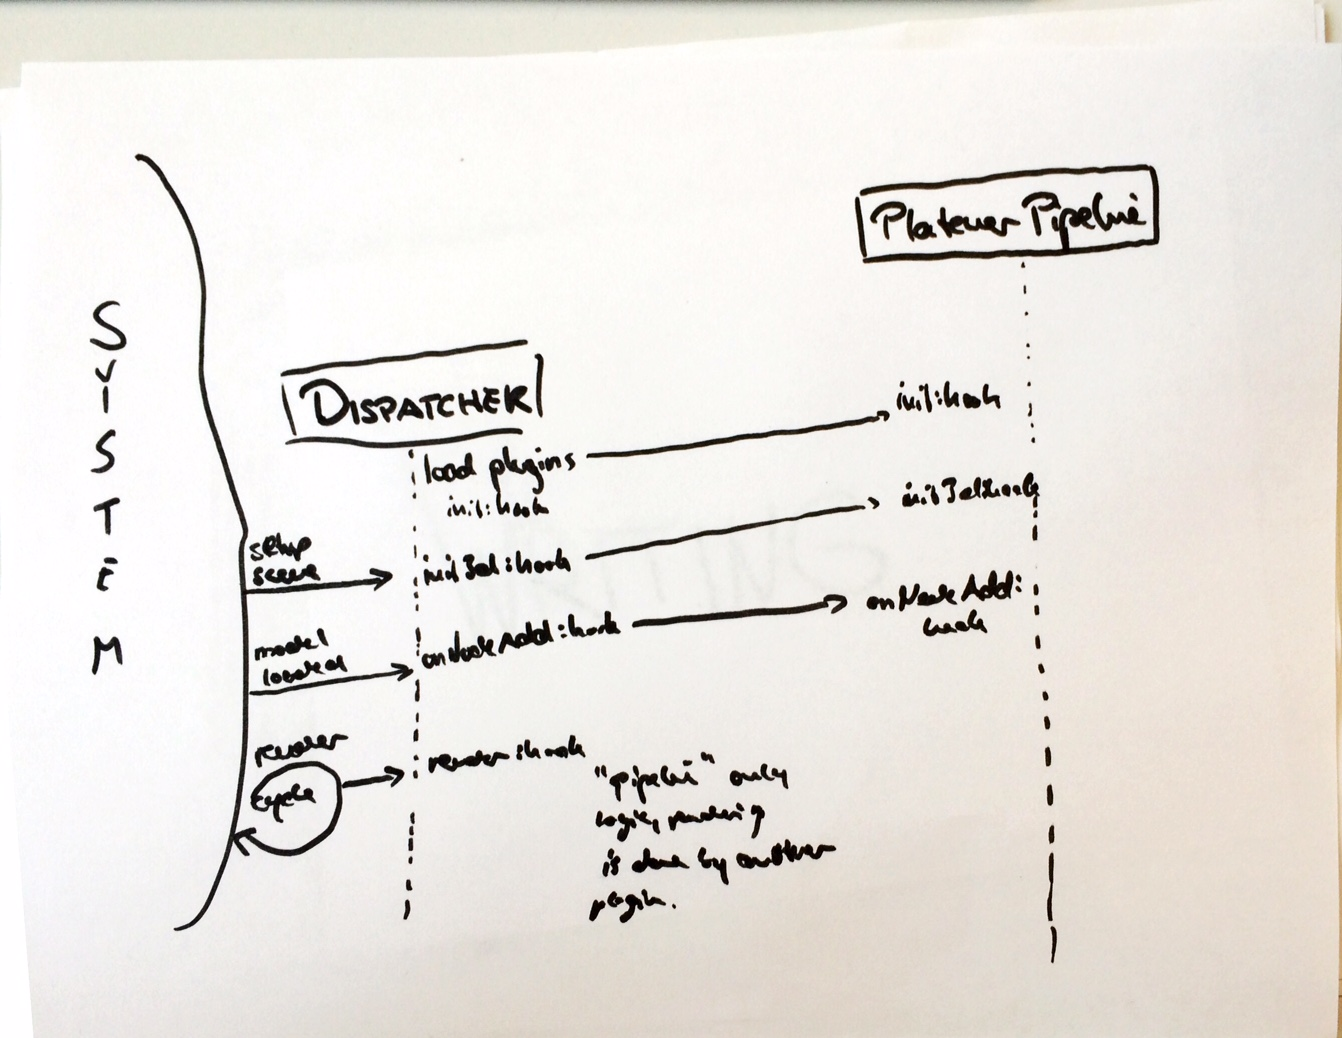
\includegraphics[width=1\columnwidth]{03-architecture_dispatcher_pipeline}
\caption{Dispatcher and PlatenerPipeline communicate via lifecycle events.}
\label{fig:architecture_dispatcher_pipeline}
\end{figure}

To allow communication between plugins themselves or plugins and Client, we use
\emph{Protocols} because \emph{PluginHooks} are not flexible enough. A
\emph{Protocol} defines an interface, which has to be implemented by a
\textit{delegate}. Via
delegation\footnote{\url{http://best-practice-software-engineering.ifs.tuwien.ac.at/patterns/delegation.html}}
we define callbacks which are invoked by Plugins on the Dispatcher. The
Dispatcher then notifies server, client or other plugins. Furthermore,
\emph{Protocols} can add a set of methods to the Dispatcher via meta
programming.

Listing \ref{lst:solutionselectiondelegate} shows the definition of the
SolutionSelectionDelegate protocol. It requires its implementing class to
provide the methods \textit{evaluationDidStart},
\textit{evalutionOfMethodDidFinish}, \textit{evaluationDidFinish},
\textit{evaluationDidFail} and \textit{evaluationDidFailWithSolutions}. Listing
\ref{lst:client_dispatcher_protocol} shows the \emph{ClientDispatcher} implementing the
\textit{evaluationDidFinish} method. By providing the callbacks, the Dispatcher
knows about the current state of the conversion and its completion. For example,
we render all solutions after their computation. To satisfy the
SolutionSelectionDelegate protocol, the Dispatcher also implements the remaining
methods.

\begin{listing}[!h]
\centering
\begin{minted}[
linenos
]{coffeescript}
SolutionSelectionDelegate = {
  shouldImplement: [
    # Invoked before a method is evaluated.
    'evaluationDidStart'
    # Invoked after each method finished.
    'evaluationOfMethodDidFinish'
    # Invoked after all methods finished.
    'evaluationDidFinish'
    # Invoked when an error occured in solution selection.
    'evaluationDidFail'
    # Invoked when errors occur in pipeline steps during computation
    'evaluationDidFailWithSolutions'
  ]
}
\end{minted}
\caption{\emph{SolutionSelectionDelegate} protocol definition}
\label{lst:solutionselectiondelegate}
\end{listing}

\begin{listing}[!h]
\begin{minted}[
linenos
]{coffeescript}
class Dispatcher extends AbstractDispatcher
  ### Solution Selection ###
  @protocol(SolutionSelectionDelegate)

  #
  # ... more protocol methods ...
  #

  evaluationDidFinish: (solutions) ->
    @getPlugin('node-visualizer').render(solutions)
\end{minted}
\caption{\emph{ClientDispatcher} implements the \emph{SolutionSelectionDelegate}
  protocol}
\label{lst:client_dispatcher_protocol}
\end{listing}

% https://developer.apple.com/library/ios/documentation/General/Conceptual/DevPedia-CocoaCore/Delegation.html
% \textbf{protocols}
% \begin{itemize}
% \item communication between packages (no lifecycle)
% \item use protocols (explicit definition of what will happen)
% \item protocol embodies a set of feature for the application
% \end{itemize}


\subsubsection{The Dispatcher is the Single Source of Truth}
\label{sec:disp-single-source}

When applications grow, it is hard to observe all messaging between components
at once. With the \emph{Dispatcher}, we control all communication between the
packages at one place. Without implicit ordering of callback executions, we can
trace erroneous behavior fast. The design of a singleton controlling the
application's lifecycle is known from frameworks in mobile application
development, like Android\ref{??} or iOS\ref{??}.

The usage of \emph{Protocols} helps developers keep track of interfaces between
components. We enforce this concept, because \javascript is a dynamically typed
programming language. Statically typed programming languages pay out, when
projects grow large. Unexpected type and interface errors happen less often.
Because of the web-environment and previous work, we are bound to \coffeescript.
Thus, we emphasize explicit structuring of interfaces via \emph{Protocols}.

% \begin{itemize}
% \item one guy who pulls all the strings (one source of truth)
% \item look up all communications between decoupled components here
% \item similar designs in known application frameworks (android, ios)
% \item javascript, non-type language --> protocols ensure correct interfaces
% \end{itemize}

%\begin{itemize}
% \item implements protocols for plugins (show code snippets)
% \item explain how plugins push state (control-flow information) back to the
%   dispatcher
%\end{itemize}

\begin{figure}
  \centering
  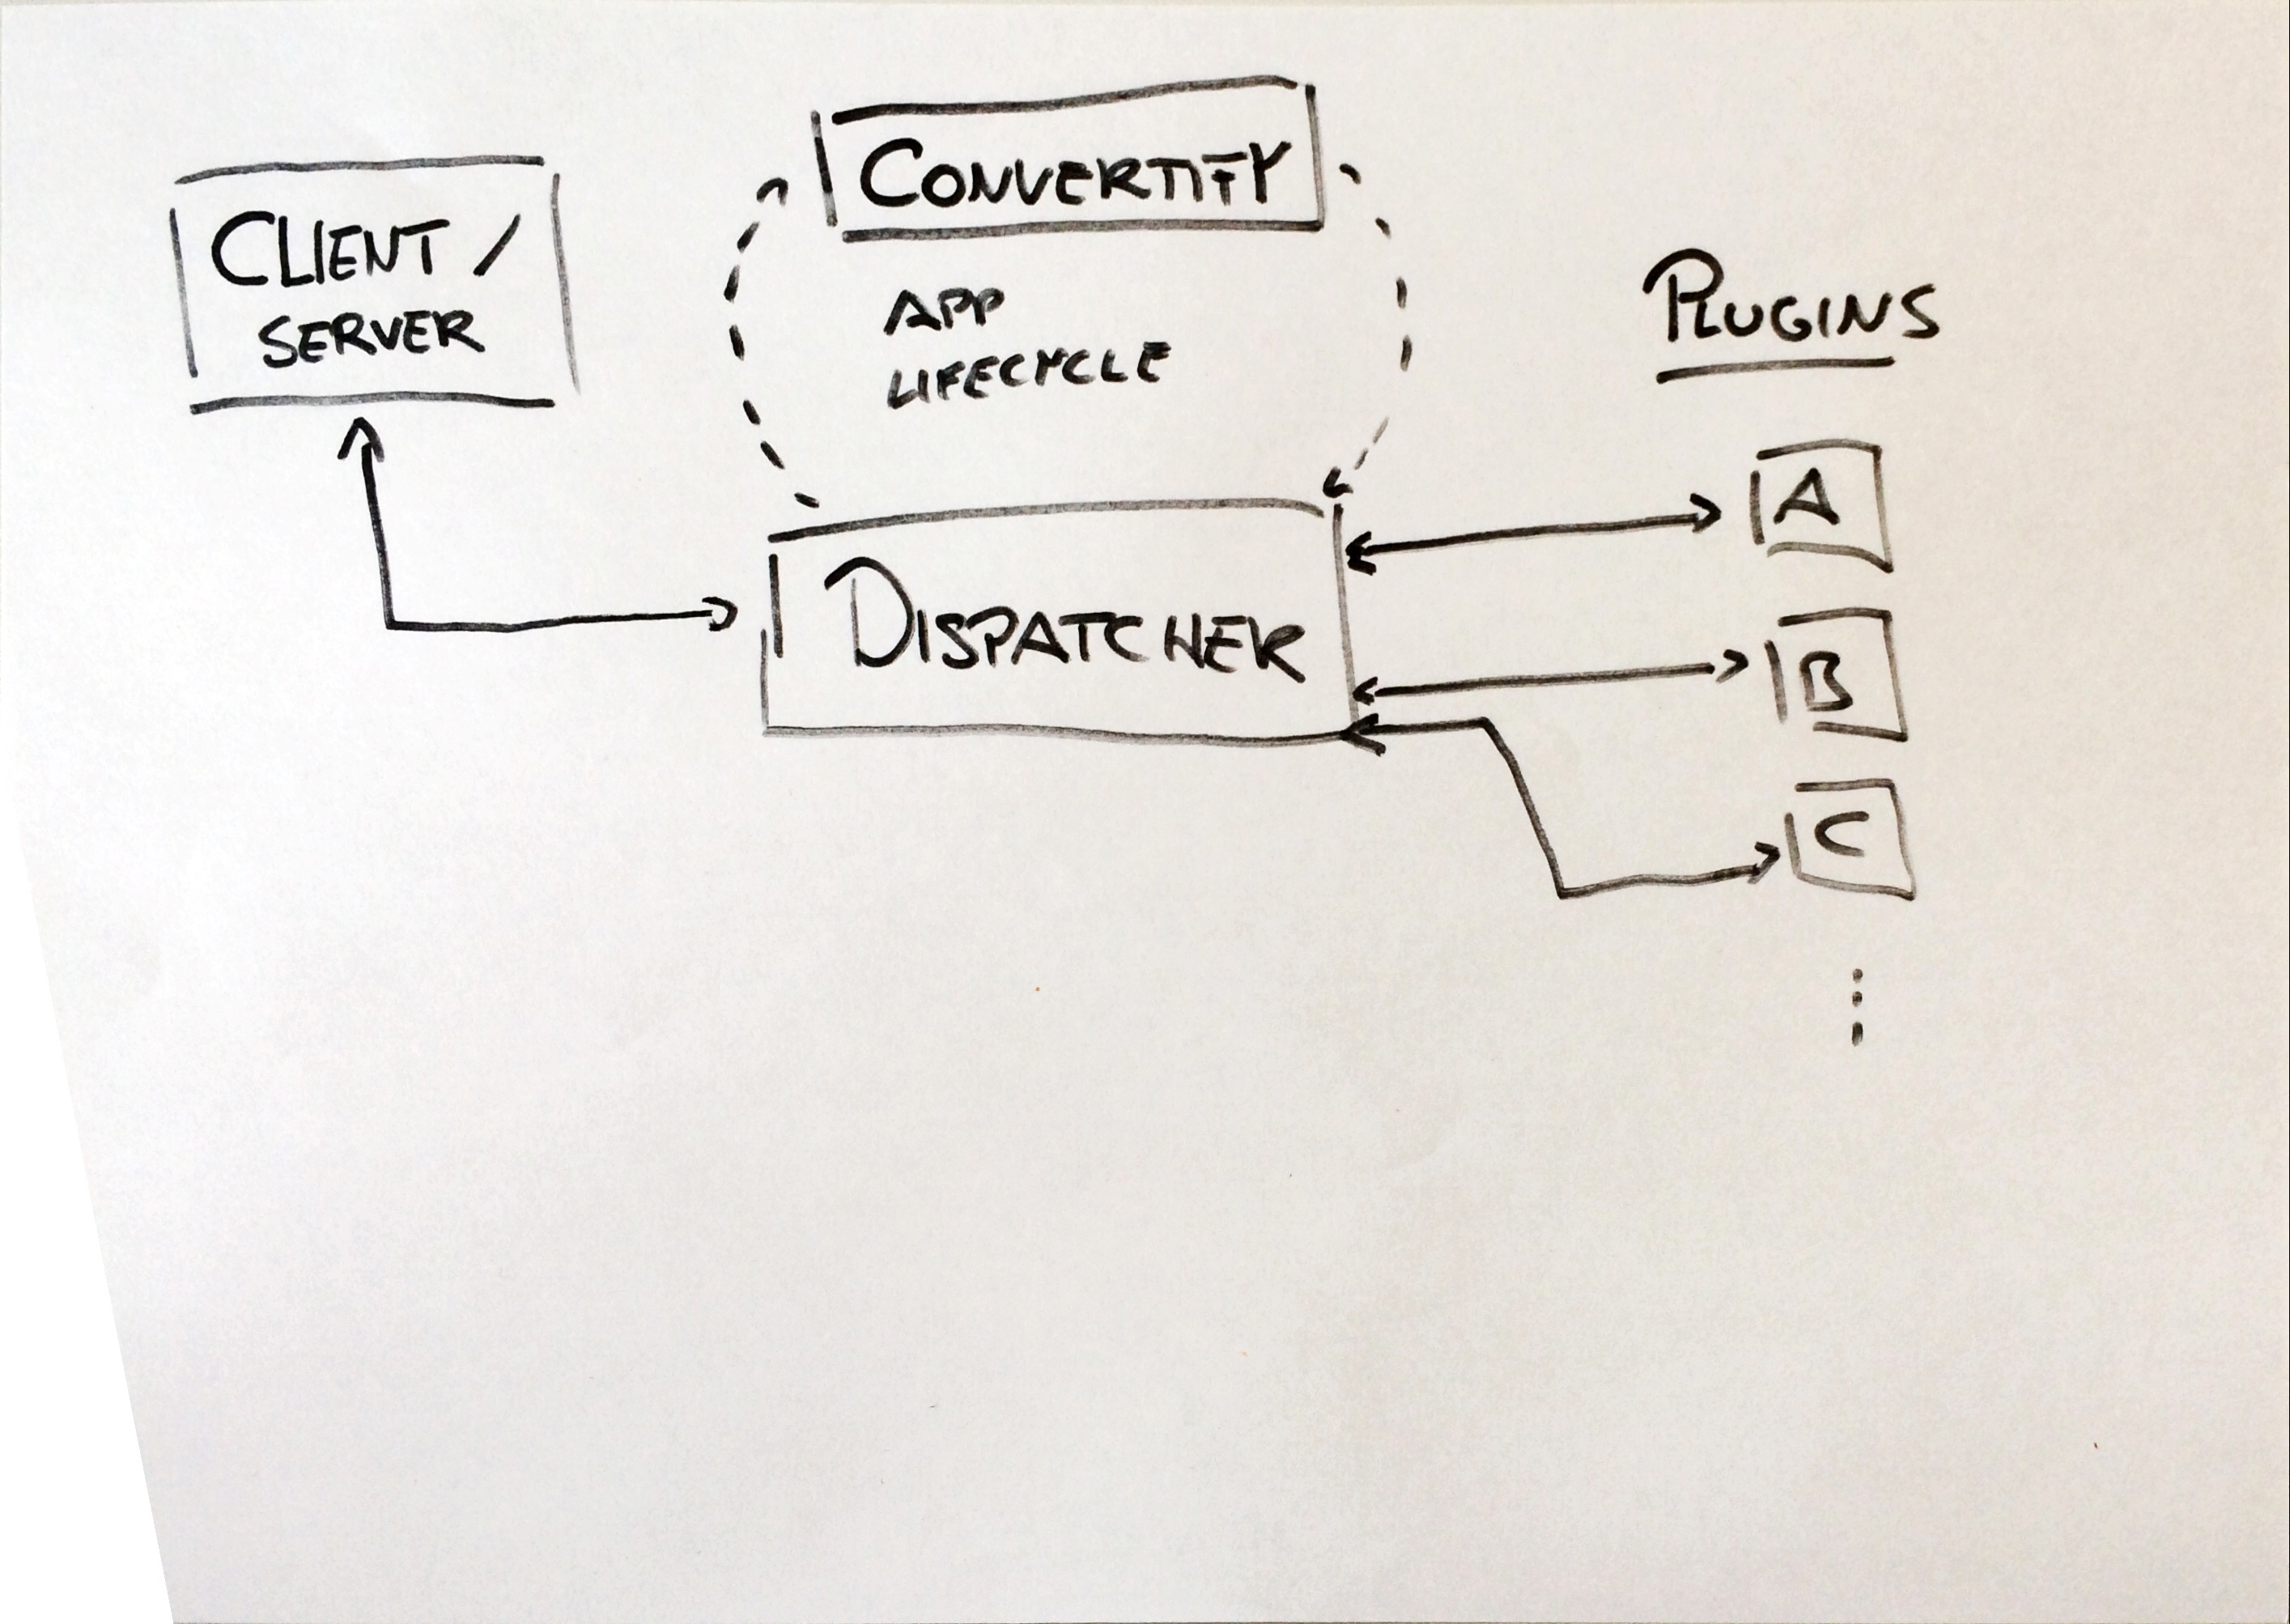
\includegraphics[width=1\columnwidth]{03-architecture_overview_dispatcher}
  \caption{Dispatcher manages inter-application communication during the
    lifecycle of the app.}
  \label{fig:architecture_overview_dispatcher}
\end{figure}

\subsubsection{Dispatcher and Bundle on Client and Server}

\myNotes{maybe put this up, so we understand earlier what the ClientDispatcher
  is}

The Server and Client package handle lifecycle events differently and use
different protocols. That is because the Client package has to handle rendering
and user interaction. The Server package merely computes the manipulated models
and is used for batch processing of {\threedmodel}s. Therefore, we need two
Dispatcher implementations for the client and for the server.

A Bundle is the entry point for any client or server code. As the name
indicates, a Bundle bundles all application code into a single instance. It
references the specific \emph{ClientDispatcher} or \emph{ServerDispatcher},
which are implemented in the Client or Server package respectively. Thus we can
control the system by invoking protocol interfaces. The ClientBundle is exposed
to the Client package. The ServerBundle is exposed to the ServerPackage.

\subsubsection{Brickify uses PluginHooks only}

\emph{Brickify} dispatches plugin hooks directly from the internal system to the
plugins without using a mediator in between. Compared to \emph{Convertify}, it
does not require any boilerplate code to setup the communication.
\emph{Convertify} needs a custom integration of each \emph{Plugin} into its
\emph{Disptacher}.

On the other hand, \emph{Brickify} could not control the ordering of
\emph{PluginHook} invokations. It is implicitly defined by the loading sequence
of plugins. Furthermore, the frontend code needs to access plugin data. The data
is only available after the plugins are loaded or even specific hooks were
executed. Via a mediator we can notify the frontend about state changes, rather
than asyncronically trying to poll the data.

With the introduction of a \emph{Dispatcher}, \emph{Plugins} now can push state
back to the system and implement \emph{Protocols} for more control over the
communication.

% \begin{itemize}
% \item wiring up plugins
% \item explicitly calling plugin hooks
% \item highly customizable when adding in new plugins
% \item how is control flow achieved? -->
% \end{itemize}

% \begin{itemize}
% \item ++ pros
% \item loading sequence control (impossible to repair)
% \item fine grained scheduling of communication
% \item explicit execution behavior
% \item ... (look at notes on desk)
% \item
% \item -- cons
% \item boilerplate code
% \item custom integration for each plugin
% \end{itemize}

% \begin{itemize}
% \item ++ pros
% \item no further config needed
% \item
% \item -- cons
% \item implicit order
% \item in different use cases, different plugins have to interact first (order is
%   not fixed)
% \item frontend often has to work on data which is not available before another
%   plugin loaded
% \end{itemize}

% \myNotes{now plugins can...}

% \begin{itemize}
% \item push application state back to the dispatcher
% \item communication with each other by specifying a protocol which has to be
%   implemented on the mediator
% \item mediator then can oversee the communication
% \end{itemize}

\section{Plugins in Platener}
% ************************************************

\subsection{Plugin Overview}

% The Client package provides the look and feel of Platener. The Server package
% manages communication between frontend and data storage.

The plugins composed into Platener provides its computation logic and WebgGL
scene rendering. We will give a brief introduction of each plugin in the
following paragraphs.

\subsubsection{Coordinate System}

This plugin provides orientation enhancements for the WebGL scene. Rendering
xyz-axes and a an axis-aligned grid, users can grasp alignment and dimensions of
{\threedmodel}s. Figure \ref{fig:architecture_overview_coordinate_system} shows
the coordinate system in the WebGL view. The Coordinate System is taken from
\emph{Brickify} as is\footnote{ref original code file}.

\begin{figure}
  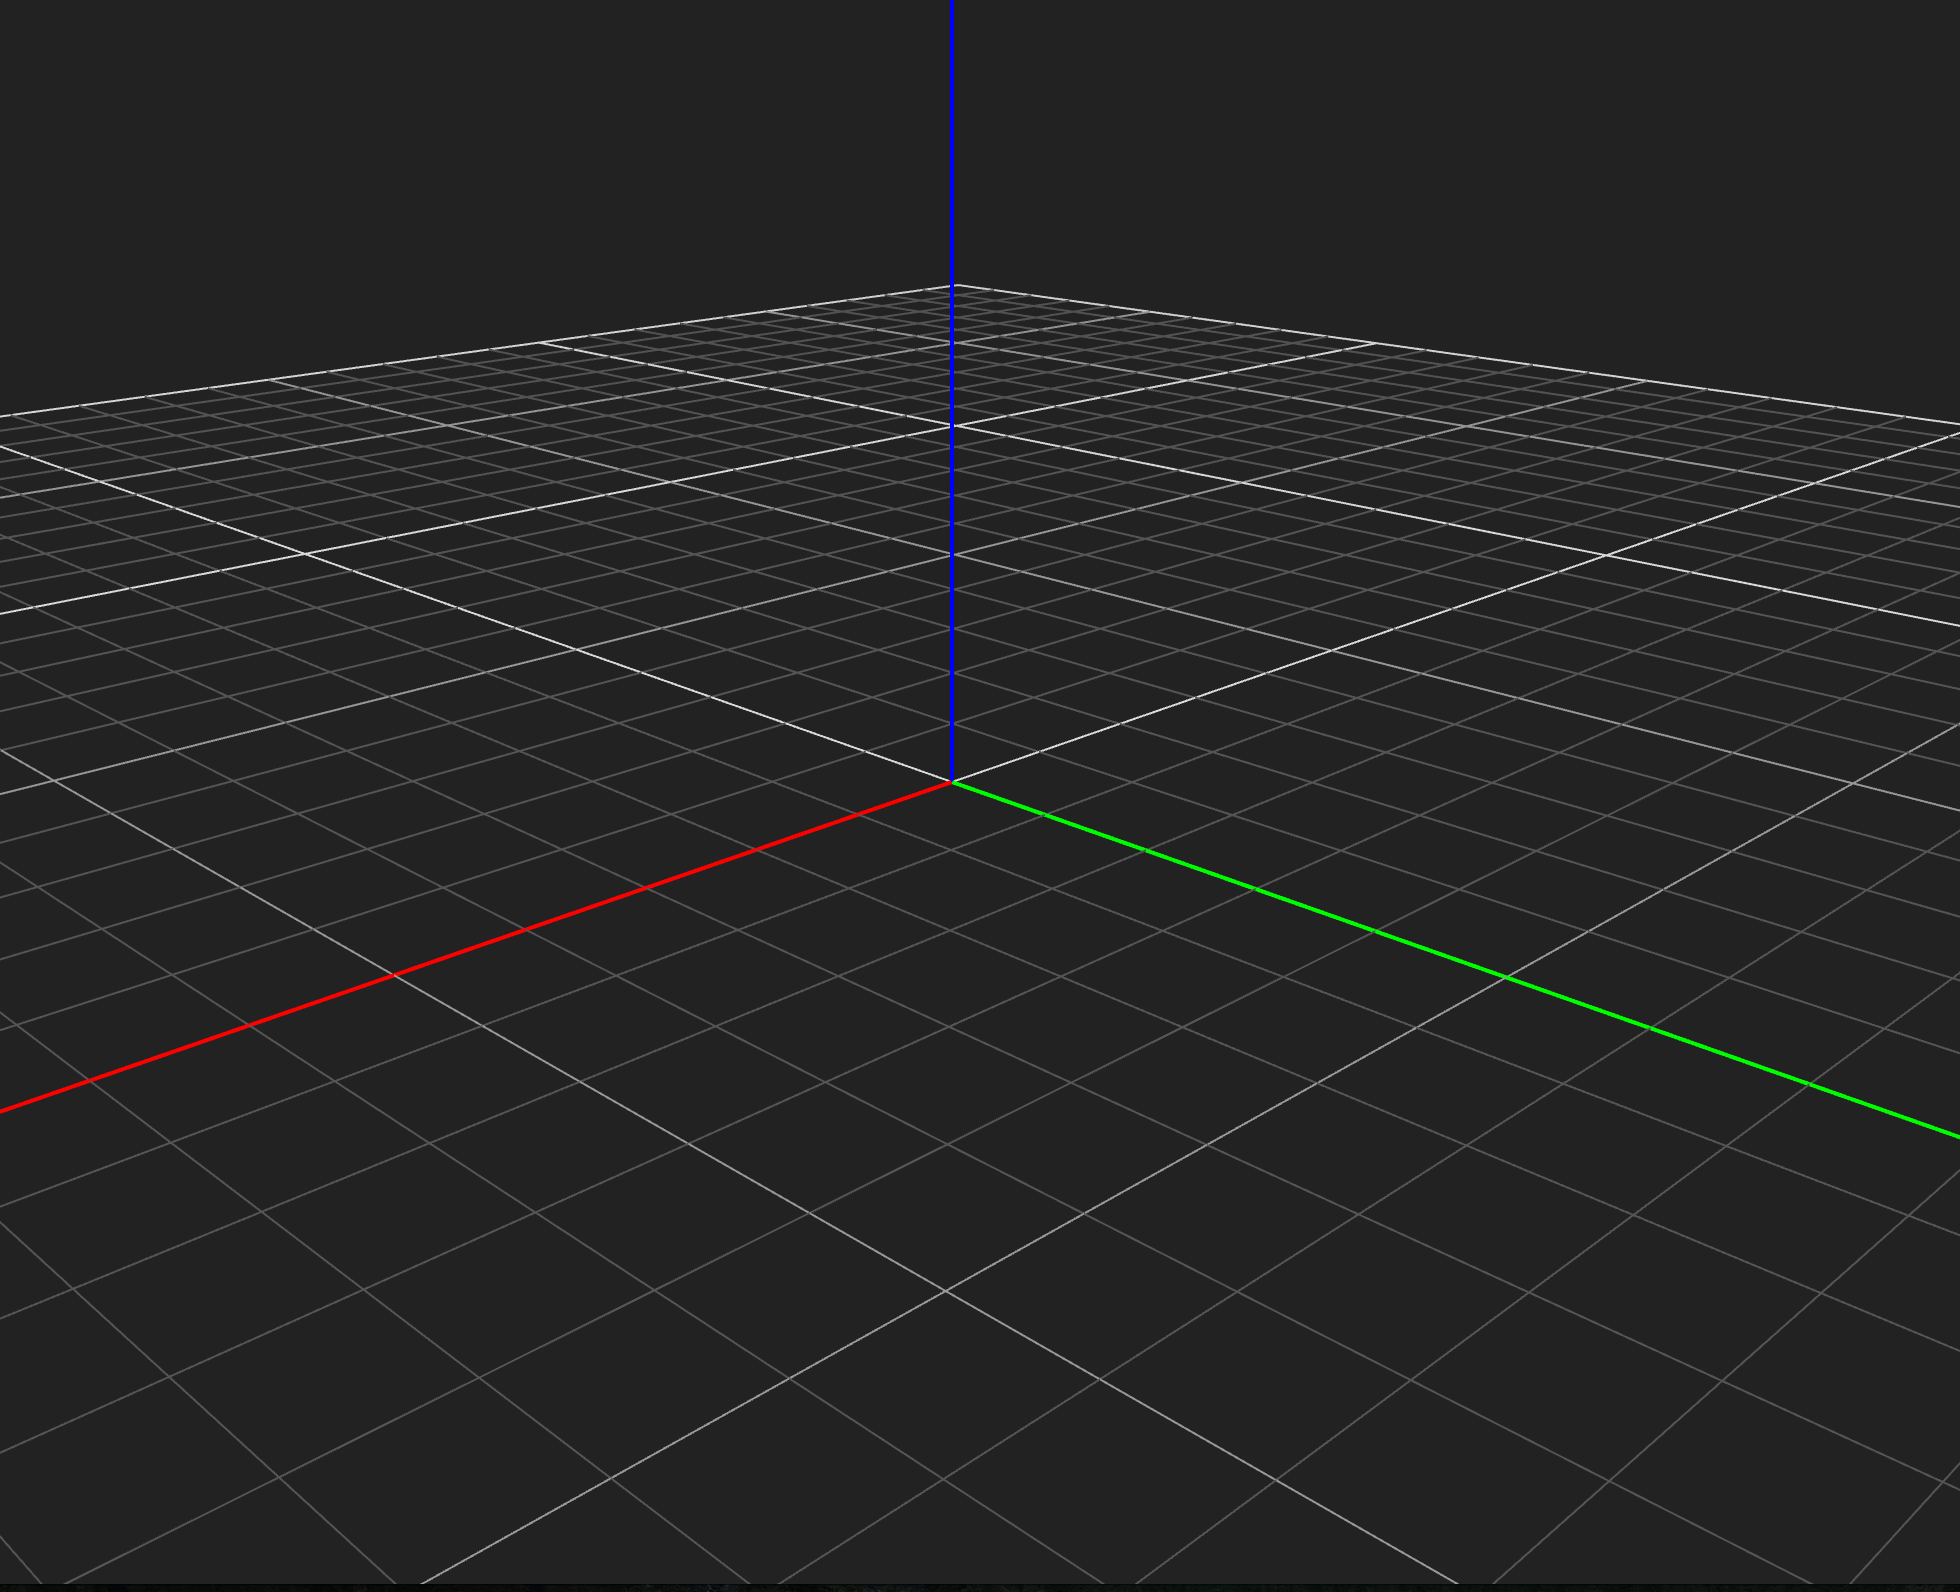
\includegraphics[width=1\columnwidth]{03-architecture_overview_coordinate_system}
  \caption{An empty scene showing the coordinate system.}
  \label{fig:architecture_overview_coordinate_system}
\end{figure}

\subsubsection{Platener Pipeline}

The Platener Pipeline plugin is the main computation unit. The plugin defines
multiple {\fabmethod}s. A {\fabmethod} is a conversion approach of a
\threedmodel. Multiple components, which can manipulate the input model, are
chained after another to produce 2D- or 3D-output. For example construction
plans for the original input model as {\svgfile}s.

\subsubsection{Node Visualizer}

We visualize the results of the Platener Pipeline plugin in the WebGL view. The
Node Visualizer plugin renders the results of each component of each
{\fabmethod} respectively.

\myNotes{add figure of a visualized model in wireframe mode (something fancy)}

\subsubsection{Scoring}

When multiple {\fabmethod}s are run, we want to choose the best fitted
conversion as output. Thus each {\fabmethod} is scored by a method-specific
scoring algorithm. This plugin provides these scoring algorithms.

\subsubsection{Solution Selection}

This plugin utilizes the Platener Pipeline plugin and the Scoring plugin to run
and evaluate all {\fabmethod}s. It outputs the result of the {\fabmethod} with
the best score and notifies the Dispatcher.

\subsubsection{Isolated Testing}

While we worked at different stages of a linearly executed {\fabmethod} in
parallel, we needed a mechanism to test each component of the {\fabmethod}
before its preceeding or succeeding components were finished. The Isolated
Testing plugin provides an isolated environment, which allows to execute a
single component of a {\fabmethod} with pre-defined input.

% - working in parallel, while needing inputs of work in progress - validate &
% visualize test scenarios for separate pipeline steps (components of a
% \fabmethod) - provide input for a given step and compute/ render results for
% just that step


\subsection{Platener Pipeline}

\begin{enumerate}
\item Overview/ Purpose/ Plugin Structure

\item conversion strategies and logic

  \begin{itemize}
  \item logic only (ui -> other plugin, frontend)
  \item processing broken into steps
  \item composable into fabrication methods = execute steps in sequence, use
    results from previous step, to go on = conversion strategy

  \item typical pipelining problem \myNotes{look up typical pipelining problems}
  \item in general we have to: clean mesh, indexing, find structure (understand
    the model), convert structures (plates and joints), export
  \item different methods may to these things differently (stacked plates vs.
    inherent plates)

  \end{itemize}

\item Pipeline Steps

  \textbf{What are pipeline steps?}

  \begin{itemize}
  \item processing unit on model data (or abstraction of it)
  \item indepentend from each other, a single task
  \item break down problem into sequential sub problems (working with
    abstractions, generating assumptions -> understand problems better, work in parallel)
  \item improve debugging experience (trace errors in decouple computation
    units, also its hard to see how vertices are from
    looking at the memory, --> see next bullet)
  \item store state of each step separately, to later render a debugging view of
    the state (like timetravel for manipulations on the model)
  \item but keep rendering apart from logic -> NodeVisualizer
  \item isolated computing -> isolated testing (nice!)
  \end{itemize}

  \textbf{How are they used in Platener Pipeline?}

  \begin{itemize}
  \item pipe steps -> build up a pipeline from composition
  \item final result will be exported from the browser
  \item a pipeline makes up a conversion strategy
  \item conversion strategy share certain subproblems -> reusable code
  \item \myNotes{as steps solve the real algorithmic problems, we dedicated separate
    chapters to them. look at chapters ??}
  \end{itemize}

  \textbf{Where to be found in the code?}

  \begin{itemize}
  \item Plugins Package
  \item organized in subdirs (remember, separate npm package)
  \item step factories -> configure steps for different strategies, inject
    dependencies and state, lazy loading
  \end{itemize}

\item Fabrication Methods
  \begin{enumerate}
  \item Plate Method
    \begin{itemize}
    \item hull and surface constructions
    \item find plates in the model (inherent), build plates from surfaces
      (extruding)
    \item intersect plates (graphing)
    \item and join connected plates (finger joints)
    \item \myNotes{figure here}
    \item \myNotes{listing showing how to concat/ pipe steps}
    \item main parts of algorithm explain in chapters lukas, klara, dimitri, deus
    \end{itemize}

  \item Stacked Plates Method
    \begin{itemize}
    \item volume approximation
    \item stack flat plates to rebuild the object
    \item preserve form, look and feel, details
    \item loose functional aspects
    \item connect via shafts (click together) or use glue
    \item \myNotes{figure here}
    \item main parts of the algorithm explained in chapters lukas
    \end{itemize}

  \item Classifier Method
    \begin{itemize}
    \item advanced technique, combining intense mesh analysis and construction
      techniques of known geometries
    \item pros: convert noisy models, local conversions: because different local
      geometries may be better converted with different techniques, e.g. stacked
      vs. fingerjoints. we can evaluate better (scoring locally also!). global
      conversions and evaluations are error prone. classifier method could
      provide a rather robust conversion strategy. \myNotes{WHY CLASSIFIERS?}
    \item work in progress
    \item we can currently use primitive detection algorithms
    \item \myNotes{figure of detected cylinder in model}
    \item main parts of the algorithm at the end of paper (classification
      chapter, ransac stuff)
    \end{itemize}
  \end{enumerate}

\item Immutable Pipeline State

  \begin{enumerate}
  \item Overview/ Purpose
    \begin{itemize}
    \item no unwanted mutations (nice persisting of intermediate results from
      pipelinesteps)
    \item later steps work on data form previous steps
    \item code was not written immutable throughout the project -> changing data
      will result in wrong visualizations of previous steps by the node
      visualizer, because rendering performs AFTER all computations are done
    \end{itemize}

  \item Immutability
    \begin{itemize}
    \item \myNotes{explain principle. have more pros and cons.}
    \item structural data sharing -> unfortunately, not for us yet, but thats
      the concept :)
    \item http://jlongster.com/Using-Immutable-Data-Structures-in-JavaScript
    \item http://stackoverflow.com/questions/10034537/persistent-vs-immutable-data-structure
    \item enforces certain code style, mutability may be easier to write
    \item slow downs maybe (performance)
    \end{itemize}

  \item Implementation Details
    \begin{itemize}
    \item PipelineState class
    \item mutable and immutable state properties
    \item providing a clone method for stored properties, because code throughout the project shall
      not necessarily be written immutable (hard to obey, --> cg dev orientated,
      c++ is not immutable)
    \item immutable properties implement the clonable protocol
    \item provide immutable in one spot -> state creation
    \item define a schema (all props always available, having defaults) ->
      reduce faults when accessing data
    \item add listing which defines the schema for stacked plates
    \item accessing undefined values will give us a warning (again, like
      protocols enforcing interface structure, reducing faulty data access)
    \item somehow a persistence api (see stackoverflow link)
    \end{itemize}
  \end{enumerate}

\item Pipeline Implementation

  \begin{enumerate}
  \item the pipeline works as follows...
    \begin{itemize}
    \item Pipeline class
    \item pipe interface for Step factories (compare listing above, stacked method)
    \item create state factory -> use composition to persist intermediate results
      (state is later accessed by node visualizer)
    \item reduce approach -> pipe last state into next step to produce new state
    \item show a listing of pseudo code, explaining how the pipeline works
    \item benchmarking (measure time for intermediate steps vs whole processing)
    \end{itemize}

  \item it can be reused (because pipelining is a generic concept)
    \begin{itemize}
    \item classifier graph (classification method)
    \item isolated testing (injectable pipeline)
    \end{itemize}
  \end{enumerate}

\end{enumerate}

\subsection{Solution Selection}

\begin{enumerate}
\item WHAT?
  \begin{itemize}
  \item Selecting the best estimated solution by default.
  \item execute all classification methods
  \item use scorer plugin to evaluate each conversion after computation
    (globally evaluated, local converted geometries could be really bad)
  \item provide list of solutions associated with a score
  \item solution with max score is provided as default download
  \end{itemize}

\item WHY?
  \begin{itemize}
  \item strategies not mergeable in current state (would be future work to bring
    them together, like classifier method approach)
  \item so we want to select the method as default, which may has done the job
    most correctly (scoring)
  \item also scoring helps to get an idea of the quality of conversion without
    looking at the result (visually) -> used in headless mode, batch processing
    we could detect poorly converted objects to have a detailed look of what
    went wrong (getting development forward, yay!)
  \end{itemize}

\item MEASUREMENTS and HOW SCORING?
  \begin{itemize}
  \item \myNotes{look at screenshots and describe in short what we thought,
      would be nice measurements}
  \item scoring plugin: per measurement per classification method -> score
    method
  \item then adding all measuremnt scores per classification together
  \item assign score to the solution
  \end{itemize}

\item HOW SOLUTION SELECTION?
  \begin{itemize}
  \item combining plugins platener pipeline and scorer
  \item promised -> loop overall pipelines of classification methods
  \item promised -> then apply scoring
  \item when failure, catch and report nicely in evaluationDidFail hook (so
    fronend can notify users, no hard failure)
  \item results pushed back to system via evaluationDidFinish hook
  \end{itemize}
\end{enumerate}

\subsection{Node Visualizer}

\begin{enumerate}
\item Overview
  \begin{itemize}
  \item meshlib library for model representation
  \item convert meshlib face vertex mesh to three js notation
  \item render imported model and its manipulated forms with threejs
  \item use data from platener pipeline plugin
  \item the dispatcher implements solutionselectiondelegate protocol, which
    lets the node visualizer render the data after it was computed (see listing
    ??, above)
  \end{itemize}

\item Visual Debugging
  \begin{itemize}
  \item Rendering into WebGL only in NodeVisualizer
  \item other plugins could also do it
  \item but keep visualization of processed model in one place
  \item for each pipeline step, access its state data in a separate
    visualization
  \item step through, like explained in walkthrough chapter
  \end{itemize}

\item Visualizer and Visualizations
  \begin{itemize}
  \item Visualization class, constructs a drawable (THREE.object3d)
  \item injects drawable into root node of NodeVisualizer plugin
  \item Renderer will render it
  \item Visualizer class, wrapper managing visibilities of visualizations
  \item toggable through frontend
  \item visualizersets -> group visualization for a fab method (not all
    fabmethods have all steps, thus dont need all visualizations)
  \end{itemize}

\item Interwoven with Platener Pipeline
  \begin{enumerate}
  \item Role of Immutability
    \begin{itemize}
    \item \myNotes{(show example of how shapes have fingerjoints)}
    \item shapes (find outlines of possible plate geometries)
    \item fingerjoints are added to shapes in a later step
    \item shapes visualization also shows fingerjoints now (no timetravel - bad
      debugging (we cannot see if shapes did something wrong))
    \item data will not be changed if immutable (yes!!)
    \end{itemize}

  \item Extracting Intermediate Data of the Pipeline
    \begin{itemize}
    \item we access solutions (state per fabmethod)
    \item PipelineVisualization parent class
    \item convert state to plain object for fast access
    \item \myNotes{listing for PipeVis}
    \item each visualization extending pipeline viz only has to implement a
      single method, returning a drawable threejs object
    \end{itemize}
  \end{enumerate}
\end{enumerate}

\subsection{Isolated Testing}

\begin{enumerate}
\item WHY?
  \begin{itemize}
  \item validation of data/ conversion
  \item parallel working (make mock data with certain assumptions)
  \item isolated testing in real environment (test env is not representative,
    integration tests with manual evaluation (look at the visual results))
  \end{itemize}

\item Static Input
  \begin{itemize}
  \item build data like assumed for the step we test
  \item not that easy: many cross references, after certain steps, complex
    data...
  \item hard to build by hand, we had to use previous steps and serialize the
    step data
  \end{itemize}

\item Testables
  \begin{itemize}
  \item 1 step, 1 static input, certain test purpose
  \item a single integration test
  \item e.g. classify a single shape as plane in classify geometry step
  \end{itemize}

\item Implementation
  \begin{itemize}
  \item reusing concept of pipeline
  \item small changes: allow only a single step, get input from testable
  \end{itemize}

\item Conclusion
  \begin{itemize}
  \item not perfected/ technically mature
  \item mostly we evaluated by dropping in models
  \item but wrongly executed previous steps may have corrupted our assumptions
  \item thats why working out nice testables would be worth it!
  \end{itemize}
\end{enumerate}

\section{Client Package}
% ************************************************

\subsection{Overview - Custom Frontend Code}

\begin{itemize}
\item when convertify framework, client is freespace to evolve yaself
\item look and feel of the application
\item task: connect logic to ui (speak with dispatcher) and build ui
\item free choice of frontend framework (we take redux + react), but nothing
  against jquery or angular or backbone or ...
\item e.g. laser origami or brickify would choose a completely different
  implementation of client -> custom per application
\item react by facebook, redux by dan abramov, like flux architecure -> uni
  directional dataflow, explicit state changes, data driven -> reduce side
  effects and be efficient in coding and trace down errors easily
\item \myNotes{diagram which shows benefits of flux architecture vs no flux
    arch, look at intro vids for redux from dan abramov}
\end{itemize}

\subsection{React Templates}

\begin{itemize}
\item show html tree graph and how data communication goes wild when talking
  with siblings
\item ideally dumb components (dont know where data is coming from, just display
  it)
\item stateless, components directory
\item WIP: before no redux, so there are some mixed up components left :S
\item show short example how a dump component looks like, \myNotes{listing!}
\end{itemize}

\subsection{Redux Data-driven Control Flow}

\begin{enumerate}
\item Redux `dispatch` and state
  \begin{itemize}
  \item one state container
  \item functional, no side effects
  \item maybe copy or reference redux description (just explain why its awesome)
  \item injected into react via context
  \end{itemize}

\item Smart Containers
  \begin{itemize}
  \item connect to state
  \item containers know where data is from (vs dump components)
  \item fitler and preprocess raw data, setup interaction events to trigger
    actions
  \item give data and callbacks to a component (they setup the actual ui, but
    contain no visible elements themselves)
  \item \myNotes{listing show how to connect and use component from other
      listing}
  \end{itemize}

\item Manage Async Plugin Hell
  \begin{itemize}
  \item as described before, plugin data is not available on load
  \item we can use Dispatcher and redux dispatch combined
  \item protocols -> state change in plugins -> dispatch -> state change in
    frontend
  \item no polling or observing of data, fully reactive (system -> client communication)
  \item as client has access to bundle, we can call interfaces exposed by
    protocols (client -> system communication)
  \end{itemize}
\end{enumerate}

\section{Server Package}
% ************************************************

\subsection{Overview - Custom Server Code}

\begin{itemize}
\item like client, can have custom implementations
\item we have caching and cli (headless version of application)
\item requires isomorphic code: execute on client and server equally
\item \myNotes{isomorphic means...}
\item threejs, polyfills, \myNotes{...}
\end{itemize}

\subsection{Model Cache}

\begin{itemize}
\item idea: build up repository of models when users interact with it
\item taken from brickify: uploading meshlib version of model
\end{itemize}

\subsection{Test Pipeline}

\begin{enumerate}
\item WHY do we have a Test Pipeline?
  \begin{itemize}
  \item robustness tests
  \item batch processing
  \item headless version for integration with other projects
  \item failure detection because of diversity of objects
  \end{itemize}

\item Headless Conversion of Objects
  \begin{itemize}
  \item run solutionselection plugin also
  \item but dispatcher is setup a bit differently
  \item no recomputation, no grid, no visualizer
  \item scene manager will not render anything (unless, WIP we exchange webgl
    rendering with headlessgl to produce screenshots of each conversion)
  \item cli tool -> safe results into directories
  \end{itemize}

\item Reports
  \begin{itemize}
  \item = extended console logs
  \item show how conversion was going
  \item display failures, status, progress
  \item in the end: sum up + give stats
  \item WIP: current problems: not all conversions are garbage collected
    correctly, will run out of memory after some conversions -.- (maybe nobody
    has to know about that)
  \end{itemize}

\item Benchmarks
  \begin{itemize}
  \item xxx testmodels
  \item we proposed mostly stacked as the best solution
  \item too many arbitrary forms hindered plate conversion
  \item just shows conversion stats (maybe all models vs box category only)
  \item \myNotes{measure times for conversions and evaluate}
  \end{itemize}
\end{enumerate}

\end{document}

%%% Local Variables:
%%% mode: latex
%%% TeX-master: "../ClassicThesis"
%%% TeX-command-extra-options: "-shell-escape"
%%% End:

\cleardoublepage

%\part{Architecture}
% Sven or Dimitri
\subfile{Chapters/03.2-Processing_Pipeline}
%\documentclass[../ClassicThesis.tex]{subfiles}
\begin{document}

%************************************************
\chapter{Processing Pipeline / Dimitri}\label{ch:processingPipeline}
% \secauthor{DS}
%************************************************

In this chapter we give a short overview over the already mentioned processing pipeline and therewith associated data structures. The text serves as an reference point to fit the individual sections into the overall concept.

As described in chapter \ref{ch:architecture} Architecture there are three fabrication methods that implement different pipelines: \emph{Plate}, \emph{StackedPlate} and \emph{Classifier}. Each pipeline consists of pipeline steps that can be described as computation units. Each step performs an operation on the given data and provides its result for the following steps.


\section{Fabrication Methods}

\subsection{Plate}

\emph{Plate} is the default fabrication method and converts the given model to an approximation consisting of plates. The pipeline is build up of following steps in the stated order: 

\begin{itemize}
    \item MeshCleanup
    \item ModelStorage
    \item Simplification
    \item MeshSetup
    \item CoplanarFaces
    \item ShapesFinder
    \item HoleDetection
    \item InherentPlates
    \item ExtrudedPlates
    \item RemoveContainedPlatesInherent
    \item RemoveContainedPlatesExtruded
    \item PlateGraph
    \item FingerJoints
    \item AssemblyInstructions
    \item Calibration
    \item ShapeLayouter
    \item MarkupGenerator
    \item ZipGenerator
\end{itemize}


\subsection{Stacked Plate}

\emph{StackedPlate} converts the given model with plates that are stacked on top of each other. The pipeline is build up of following steps in the stated order:

\begin{itemize}
    \item MeshCleanup
    \item ModelStorage
    \item MeshSetup
    \item CoplanarFaces
    \item ShapesFinder
    \item HoleDetection
    \item StackedPlates
    \item StackedPlatesAssemblyInstructions
    \item MarkupGenerator
    \item ZipGenerator
\end{itemize}


\subsection{Classifier}

\emph{Classifier} does not produce a final conversion yet. It analyses the given model with several classifiers trying to identify the various primitives contained in the mesh. The pipeline is build up of following steps in the stated order:

\begin{itemize}
    \item MeshCleanup
    \item ModelStorage
    \item MeshSetup
    \item CoplanarFaces
    \item ShapesFinder
    \item HoleDetection
    \item LabelledShapes
    \item GeometryClassification
\end{itemize}



\section{Pipeline Steps}

\subsection*{MeshCleanup}

\emph{MeshCleanup} searches the mesh for zero faces and removes them. This ensures the mesh's two-manifoldness.


\subsection*{ModelStorage}

\emph{ModelStorage} stores the input model for easy access within the pipeline.


\subsection*{Simplification}

\emph{Simplification} takes the loaded 3D model, reduces its complexity and removes unwanted features. Therefore the processing gets easier and faster. 


\subsection*{MeshSetup}

During \emph{MeshSetup} the face-vertex mesh of meshlib is transformed into the \emph{faceVertexMesh} data structure. Then the edges and faces are traversed to built a look-up table and the corresponding reverse look-up table. These tables greatly speed up algorithms that work with the mesh data, e.g. \emph{CoplanarFaces}.


\subsection*{CoplanarFaces}

\emph{CoplanarFaces} groups faces which are both connected and coplanar, which allows the creation of more complex shapes.


\subsection*{ShapesFinder}




\subsection*{HoleDetection}

\emph{HoleDetection} takes the found \emph{shapes} and classifies their \emph{edgeLoops} either as outer contour or hole.


\subsection*{InherentPlates}

\emph{InherentPlates} searches the model for plates which consist of both a top and a bottom side which are included in the mesh.


\subsection*{ExtrudedPlates}

\emph{ExtrudedPlates} creates plates by translating shapes along their normal, resulting in two sides of a plate.


\subsection*{RemoveContainedPlatesInherent}

\emph{RemoveContainedPlatesInherent} deletes unecessary plates produced by the \emph{InherentPlates} step.


\subsection*{RemoveContainedPlatesExtruded}

\emph{RemoveContainedPlatesExtruded} deletes unecessary plates produced by the \emph{ExtrudedPlates} step.


\subsection*{PlateGraph}

The \emph{PlateGraph} analyses plate adjacencies to find intersections between plates and prepare these for connecting them.

\subsection*{FingerJoints}

The \emph{FingerJoints} step creates the desired type of joints for each previously found plate intersection and adds them to the plates. This is required so the plates can be connected without glue or screws when cut and assembled.


\subsection*{AssemblyInstructions}

Each layouted shape is labelled with numbers for each connection to another plate. These numbers help the user to find plates that need to be assembled to each other.


\subsection*{Calibration}

\emph{Calibration} offsets all outlines of all plates by half the laser cutter’s kerf. Thus we incorporate that the plates will be smaller by a tenth of a millimeter after cutting. This is necessary so we can assemble all plates without using glue or skrew.


\subsection*{ShapeLayouter}

The \emph{ShapeLayouter} arranges the shapes in the cutting plan. It tries to pack them dense to avoid waste of material.


\subsection*{MarkupGenerator}

The \emph{MarkupGenerator} receives the \emph{threejs} shapes of the \emph{ShapeLayouter} step. These shapes represent the outlines of all plates in 3D space. The pipeline step converts the \emph{threejs} datastructure into a tree of React Components. This Component tree is then rendered to SVG markup.


\subsection*{ZipGenerator}

The \emph{ZipGenerator} writes all previously generated SVG files into a ZIP file. Additionally, it collects meta data from the pipeline state and stores it as a JSON file. The meta data can be used by third party applications to reconstruct the internal data representation.


\subsection*{StackedPlates}

\emph{StackedPlates} slices the model in even intervals. By stacking the resulting plates on top of each other, the original model is approximated.


\subsection*{StackedPlatesAssemblyInstructions}

\emph{StackedPlatesAssemblyInstructions} enumerates all plates, telling the user in which order they should be assembled.


\subsection*{LabelledShapes}

Each shape is transformed into a \emph{labelledShape}. \emph{LabelledShapes} are used during \emph{GeometryClassification} to assign classified primitives to their original faces and vertices in the mesh.


\subsection*{GeometryClassification}




\section{Data Structures}

\subsection*{Mesh}

\emph{Mesh} is the data that represents the complete 3D model which is loaded into our system. It contains the triangles a model is made of. Concretely the specific points and edges of the geometry.

\subsection*{FaceVertexMesh}

\emph{FaceVertexMesh} is the data object produced by \emph{meshlib} which is responsible for the model import. We improve the data by adding indices which results in faster operations. Furthermore it contains the information to map altered or newly generated points and faces to the original geometry.

\subsection*{Shape}

A \emph{shape} is a flat 2D surface in 3D space. It contains \emph{edgeLoops} that represent outer contour and holes. It is used to build up \emph{plates}. Furthermore it provides the functionality to represent its \emph{edgeLoops} in 2D space which is needed for several oparations like joint generation.

\subsection*{EdgeLoop}

An \emph{edgeLoop} contains set of connected edges all lying in a plane in 3D space. The edges are implicitly given by the stored vertices.

\subsection*{Plate}

A \emph{plate} is a \emph{shape} with a thickness and therefore a three dimensional object instead of a 2D surface.

\subsection*{Polygon}

A \emph{Polygon} is a set of vertices in 2D space used in \emph{PlateGraph} and finger joint generation. General generation of new geometry is done in 2D space, therefore 3D data is transformed into \emph{polygons} and retransformed into 3D space when the operations are finished.

\end{document}
\cleardoublepage

%\part{Approximation}
% Dimitri
\subfile{Chapters/04-Approximation}
%\documentclass[../ClassicThesis.tex]{subfiles}

\newcount\colveccount
\newcommand*\colvec[1]{
        \global\colveccount#1
        \begin{pmatrix}
        \colvecnext
}
\def\colvecnext#1{
        #1
        \global\advance\colveccount-1
        \ifnum\colveccount>0
                \\
                \expandafter\colvecnext
        \else
                \end{pmatrix}
        \fi
}

\begin{document}

%************************************************
\chapter{Approximation}\label{ch:approximation}
% \secauthor{DS}
%************************************************

\newcommand\myNotes[1]{\textcolor{red}{#1}}


In this chapter we describe our methods to reduce the complexity of our data.

The pipeline step \emph{Simplification} provides a simplified version of the {\threedmodel} for all subsequent processing steps. The operation is called mesh simplification. This processing step serves two purposes: Removal of unwanted details and runtime improvement.

The implemented mesh simplification is called vertex welding. It is also reused in other processing steps of our software to remove unnecessary vertices.

Furthermore we eliminate obsolete vertices during shape generation with point on line removal.


\section{Mesh Simplification}


Mesh simplification reduces the complexity of a {\threedmodel} by decreasing the amount of vertices and faces. In this process the original object gets approximated with less information. While doing so the differences between the processing results of an original and an approximated object are kept as low as possible.

Our mesh simplification tackles three issues:

\paragraph*{Processing Time}

After the model is loaded and stored we decrease its complexity to speed up following processing tasks. Every pipeline step benefits from this mesh simplification because of the reduced data they are working on which implicates a much faster pipeline runtime.

\paragraph*{Abstraction}

Furthermore we eliminate beveled edges that are not functional but created by 3D-modeling software because of aesthetic reasons. These can be removed since they do not serve any functionality and raise the complexity for conversion. The vertex welding approach gives us the needed shape abstraction to extract tiny details and minor curvatures we do not want to reproduce.

\paragraph*{Elimination of redundant information created by our processing pipeline}

The algorithm can be reused in further processing to ensure unambiguous vertices that may occur due to rounding differences during transformations.


The used technique is known as 'vertex welding' in computer graphics: We merge two or more vertices that lie in a specified distance to each other. Then the mesh contains fewer vertices. As a consequence of the smaller vertex set, thin faces no longer consist of three distinct vertices: Two nearby vertices are just represented by one vertex and the face gets deleted.

To illustrate the method the {\threedmodel} Stanford Bunny shown in Figure \ref{fig:origBunny} is simplified with an unusually high welding distance of 10mm in Figure \ref{fig:10mmBunny}. The images display each face with a different color to visualize the resulting face set. The loaded model consists of 8662 faces while the simplified bunny is reduced to 616 faces. Note, how smaller details like eyes and ears get lost with higher welding distance while the overall shape still remains. For effect illustration the welding distance is higher than the actual distance for processing.

\begin{figure}
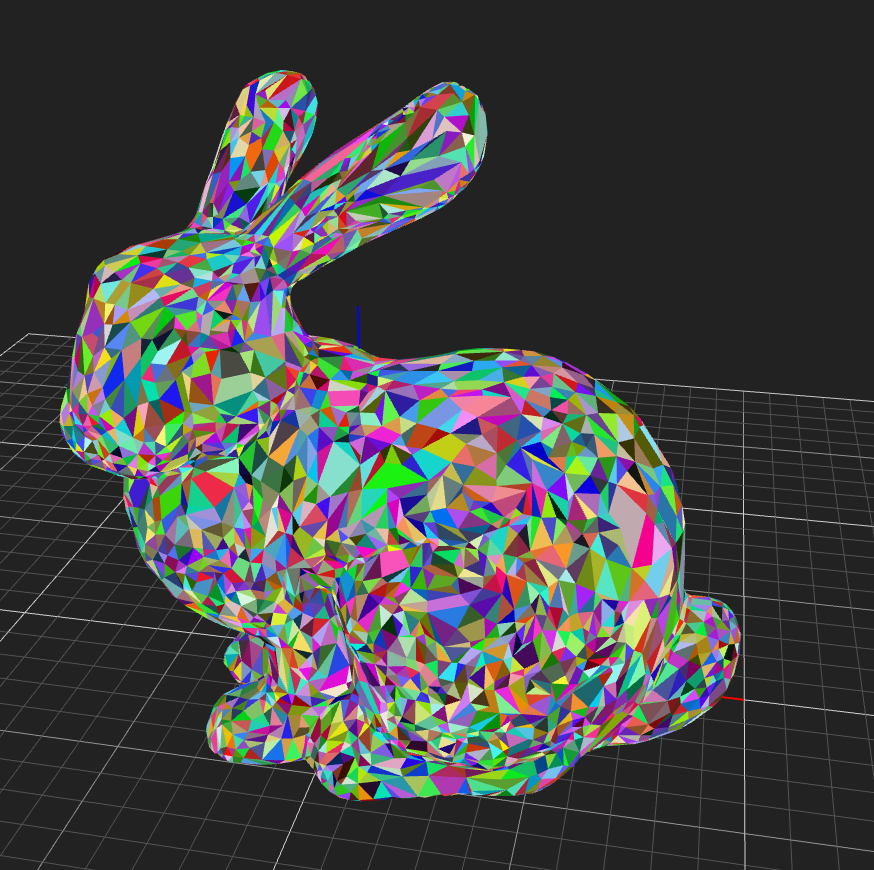
\includegraphics[width=0.8\columnwidth]{Images/04-approx-welding-rabbit-original.png}
\caption{Stanford Bunny with 8662 faces}
\label{fig:origBunny}
\end{figure}

\begin{figure}
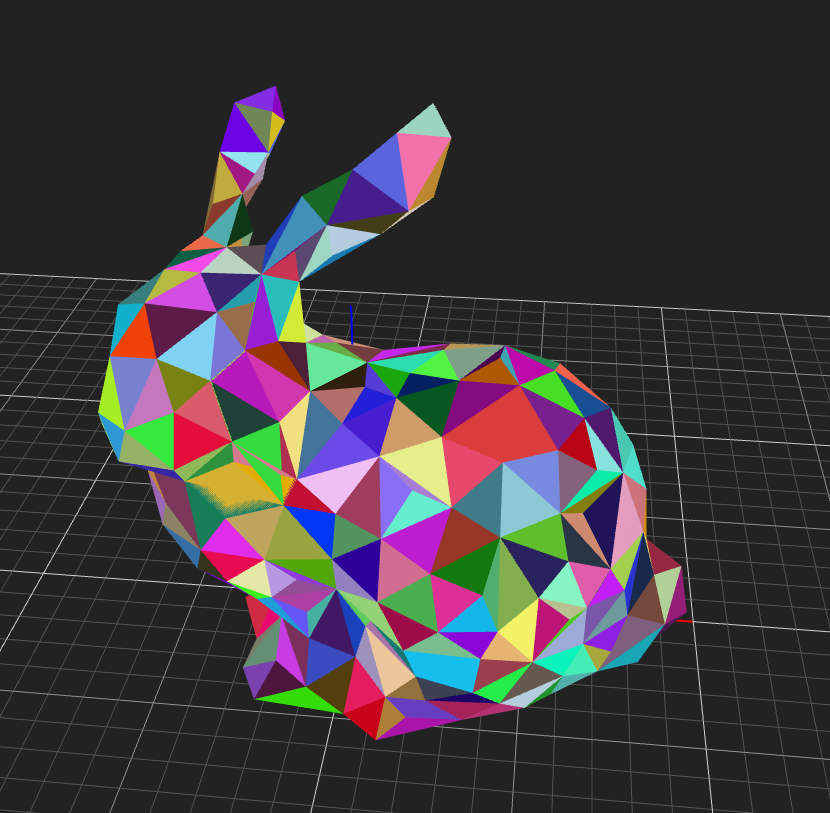
\includegraphics[width=0.8\columnwidth]{Images/04-approx-welding-rabbit-10mm.png}
\caption{Simplified Stanford Bunny with 616 faces (welding distance: 10mm)}
\label{fig:10mmBunny}
\end{figure}




\subsection{Vertex Welding}
\label{sec:vertex_welding}

% Überblick

% 2 Modi -> preprocessed, first come


% Algorithmus erklären...


% Hase

% Beveled edges



Vertex Welding merges vertices and works as shown in Figure \ref{fig:vertex_welding}:

A set of triangles is given. We choose a welding distance so points that lie further away of each other will not get merged. This is also the maximum distance a merged vertex can be away from its original position. Therefore it describes the variance of input and resulting vertex set.

For each cluster of vertices that gets merged, a new vertex is created which is typically in the middle of all corresponding points. The original vertices are replaced by this new one in each triangle.

In case a triangle $ABC$ has two points in the same merge cluster $A$ and $B$, both get replaced by the new vertex $V$. As a result the triangle consists of the points $VVC$ while it does not contain three distinct vertices anymore - it is a line. If all three of its points lie in a cluster the outcome triangle $VVV$ is a single point. In these cases the triangle gets deleted. The initial area of these deleted triangles is now covered by its adjacent triangles.

The result is an approximation of the input with fewer vertices and faces while the maximum variance equals the specified welding distance. As illustrated in Figure \ref{fig:vertex_welding}, the resulting shape can also completely equal the original one without any differences: Only vertices inside the rectangle got merged which does not affect the outline of the object.



\begin{figure}
\includegraphics[width=0.8\columnwidth]{Images/04-approx-welding-overview2.png}
\caption{Vertex Welding}
\label{fig:vertex_welding}
\end{figure}

\subsubsection{How the vertex algorithm is esed in our software}

For each welding application a new instance of \emph{VertexWelding} is created with the desired welding distance. Then, the data can be preprocessed before the actual welding which provides the best possible result. Each vertex is then replaced by the \emph{VertexWelding} vertices. The points can be merged without preprocessing in case it is not needed (for instance while using very small welding distances).

\emph{VertexWelding} provides five functions:

\subsubsection*{preProcessModel}

preprocesses the given meshlib model.

\subsubsection*{preProcessVertices}

preprocesses the given array of vertices. A Vertex may be any object containing \emph{x}, \emph{y} and \emph{z} values.

\subsubsection*{preProcessVertex}

preprocesses the given vertex which may be any object containing \emph{x}, \emph{y} and \emph{z} values.

\subsubsection*{getCorrespondingVertex}

returns a new vertex based on the given one. This function is called for replacing each point of your object.

\subsubsection*{replaceVerticesAndDeleteNonTriangularFaces}

handles the welding process for the given meshlib model: It replaces all vertices and deletes triangles that are not needed any more.


So a set of vertices is welded by calling \emph{preprocessVertices}, iterating over all points and replacing them with the vertex from \emph{getCorrespondingVertex} or just replacing them without preprocessing.


\subsubsection{Implementation}

\emph{VertexWelding} builds a list of weighted vertices during preprocessing. All original points are replaced with these \emph{weightedVertices} during the welding process so this list contains all vertices that end up in the resulting dataset.

During list setup each new vertex is either merged with an existing \emph{weightedVertex} or added to the list. Therefore all original vertices are represented by a \emph{weightedVertex}. A \emph{WeightedVertex} saves the number of represented points to merge new vertices correspondingly as shown in Figure \ref{fig:weightedVertex}.

In this figure point 1 is a \emph{weightedVertex} with $weight = 2 $. Point 2 is the next vertex to be preprocessed and is within welding distance to point 1. Therefore point 2 is merged with point 1. The resulting point 3 lies between point 1 and 2. Since point 1 has $ weight = 2 $ the distance between point 3 and 1 is half the distance between point 3 and 2.

\begin{figure}
\includegraphics[width=0.4\columnwidth]{Images/04-approx-WeightedVertex.png}
\caption{Point 3 is the result of merging point 1 and 2. Point 1 is a weightedVertex with weight = 2}
\label{fig:weightedVertex}
\end{figure}

After preprocessing all points of a given set have to be replaced while \emph{getCorrespondingVertex} returns the respective vertex for each requested point.

In case a point is requested without preprocessing \emph{VertexWelding} builds its list without putting the new vertex in between the merged points but picks the first one as representative for all following.




\paragraph{Preprocessing}

Preprocessing is done with one of the following methods:

\begin{description}
    \item preProcessModel
    \item preProcessVertices
    \item preProcessVertex
\end{description}

They iterate over the weighted vertex list and weld the new vertex with an existing one if they are in welding distance. The vertex is just added to the list, if it was not merged after complete iteration. This process is explained by listing \ref{lst:weldingLoop} which shows simplified pseudo code.

\begin{listing}[!h]
\centering
\begin{minted}[
linenos, breaklines
]{coffeescript}
preProcessVertex (newVertex) ->
    for wv in weightedVertices
        if wv.isInWeldingDistanceTo(newVertex)
            wv.merge(newVertex)
            return
    weightedVertices.push( new WeightedVertex(newVertex) )
\end{minted}
\caption{Algorithm for preprocessing a new vertex}
\label{lst:weldingLoop}
\end{listing}

Merging is done by adding a fraction of the vector between \emph{WeightedVertex} and new vertex. The fraction is based on the weight of the \emph{WeightedVertex} which is the amount of already welded vertices.

A \emph{WeightedVertex} $\vec{v}_{weighted}$ is instanced with weight $w = 1$. When a point $\vec{v}_{new}$ is added, weight gets increased and the new coordinates are computed:

$ w = w + 1 $

$ \vec{v}_{weighted} = \vec{v}_{weighted} + \frac{\vec{v}_{new} - \vec{v}_{weighted}}{w}$


\paragraph{Vertex Replacement}

The actual vertex replacement is done manually for each point with \emph{getCorrespondingVertex}, meaning \emph{VertexWelding} just provides the new vertices and does not replace the old ones. It iterates over the weighted vertex list and returns a point if it is in welding distance. After iteration it adds the vertex to its weighted vertex list in case there was no corresponding one. This automatically handles welding without preprocessing: Each passed vertex is added to the list as long there is no vertex in welding distance yet. Therefore the first vertex serves as representant for all following ones that lie nearby.

A complete model can be handled with \emph{replaceVerticesAndDeleteNonTriangularFaces}. It takes a \emph{meshlib} model and iterates over all faces. Each three points get replaced and a face get deleted if its points are not distinct anymore.




\subsection{Simplification Pipelinestep}

After the pipeline step \emph{ModelStorage} saved the unmodified {\threedmodel} \emph{Simplification} provides a simplified version for all subsequent processing steps. It is directly followed by \emph{MeshSetup} and \emph{CoplanarFaces} which analyses the given mesh to combine multiple faces.

This processing step serves two purposes: Removal of unwanted details and runtime improvement. Due to the capability of representing details with stacked plates, \emph{Simplification} is not run in \myNotes{StackedPlatesMethod (richtiger Name einzusetzen)}

\subsubsection{Details with stacked plates}

If sliced in an advantageous direction tiny details of a {\threedmodel} can be obtained with stacked plates. These details may be textures or bump maps like an engraving or a rough surface.

In general \emph{Simplification} removes such details as shown in Figure \ref{fig:3mmMakerbotMake}. With a welding distance of 3mm the result is a smooth surface while the original model shown in Figure \ref{fig:origMakerbotMake} contains the text 'Make:'.

To simplify a model without loosing such a text is not possible with the implemented vertex welding due to the nature of these texts: The labeled surface differs barely from a smooth surface. Therefore the vertices are so close to each other that welding will occur with every chosen welding distance. To obtain those texts the algorithm has to know areas where it must not weld. If you try to outline the text with a smaller welding distance there will always be some kind of artifacts: missing or degenerated letters like in Figure \ref{fig:08mmMakerbotMake}.

In order to be able to represent such texts with stacked plates \emph{Simplification} is not run in \myNotes{StackedPlatesMethod (richtiger Name einzusetzen)}


\begin{figure}
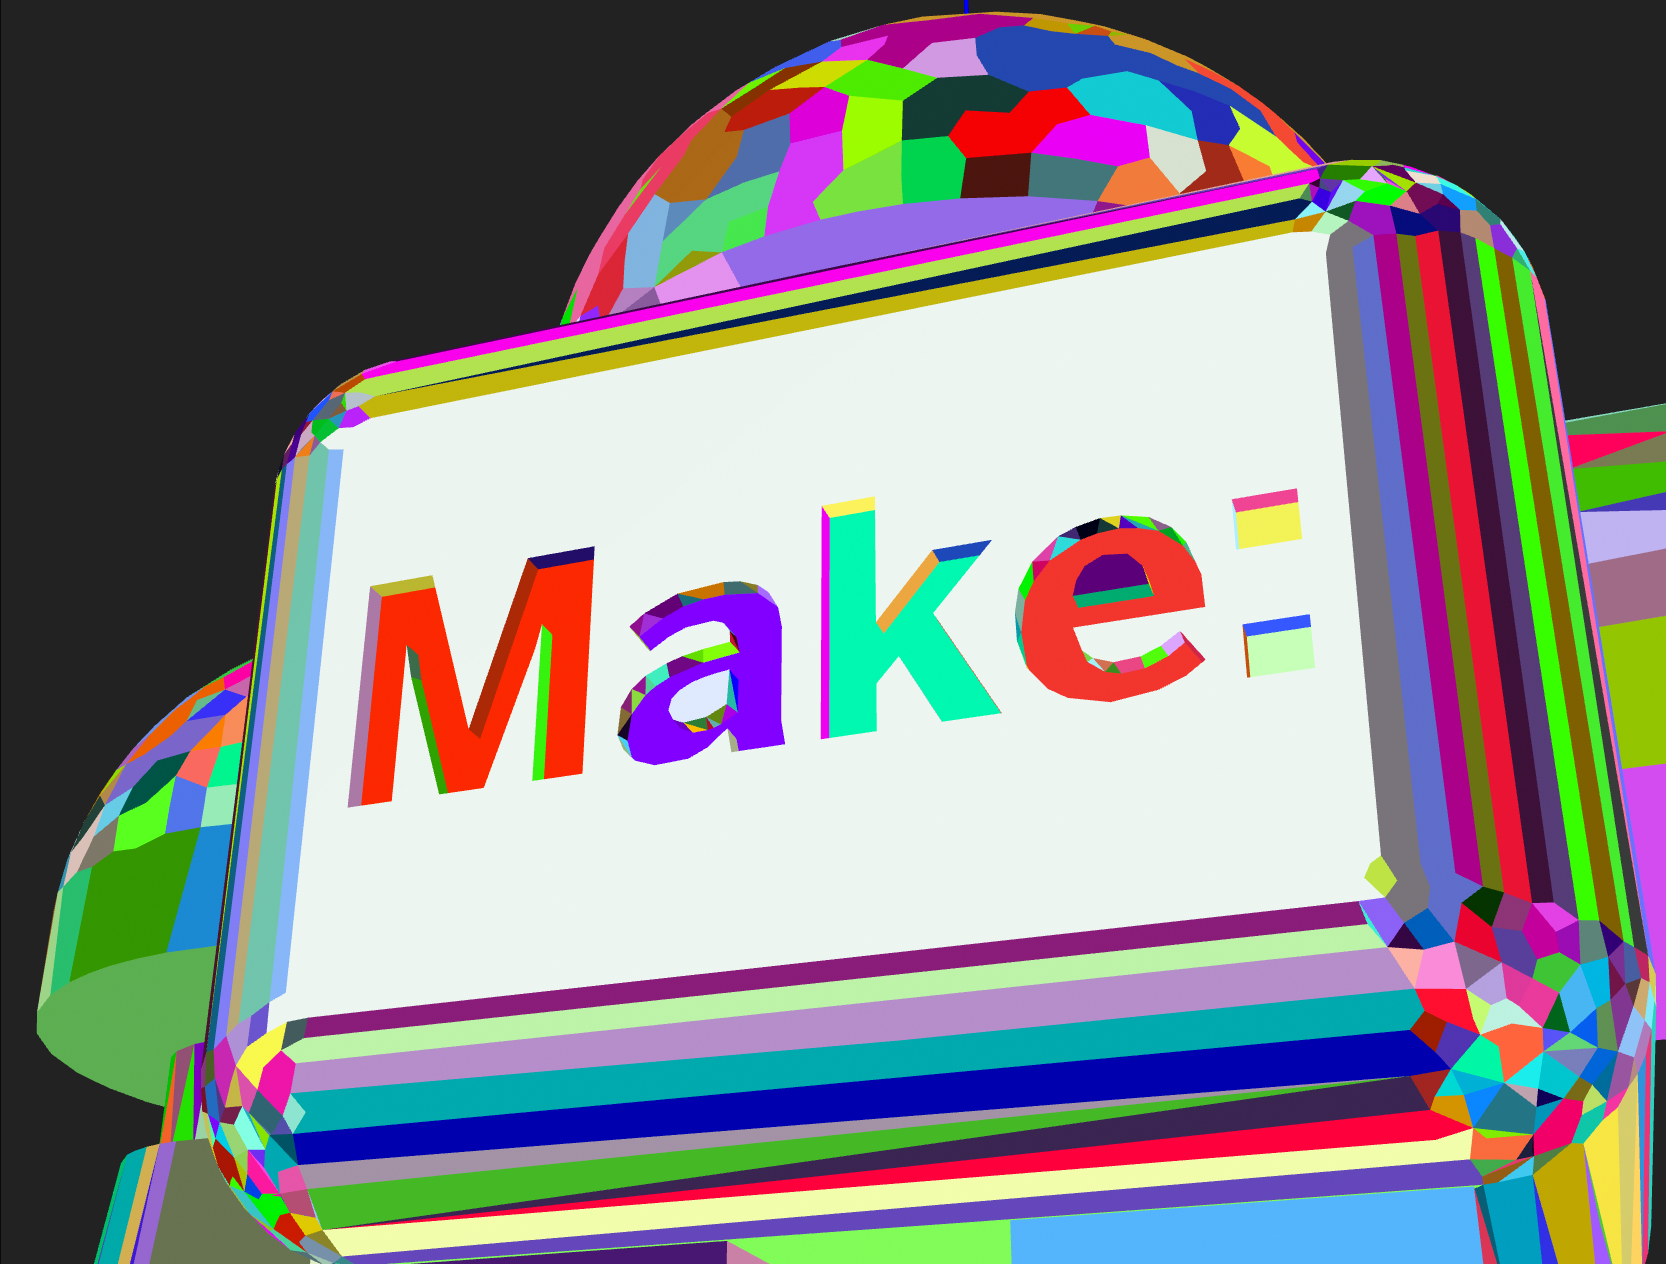
\includegraphics[width=0.8\columnwidth]{Images/04-approx-welding-make-unwelded.png}
\caption{Original Makerbot letters}
\label{fig:origMakerbotMake}
\end{figure}

\begin{figure}
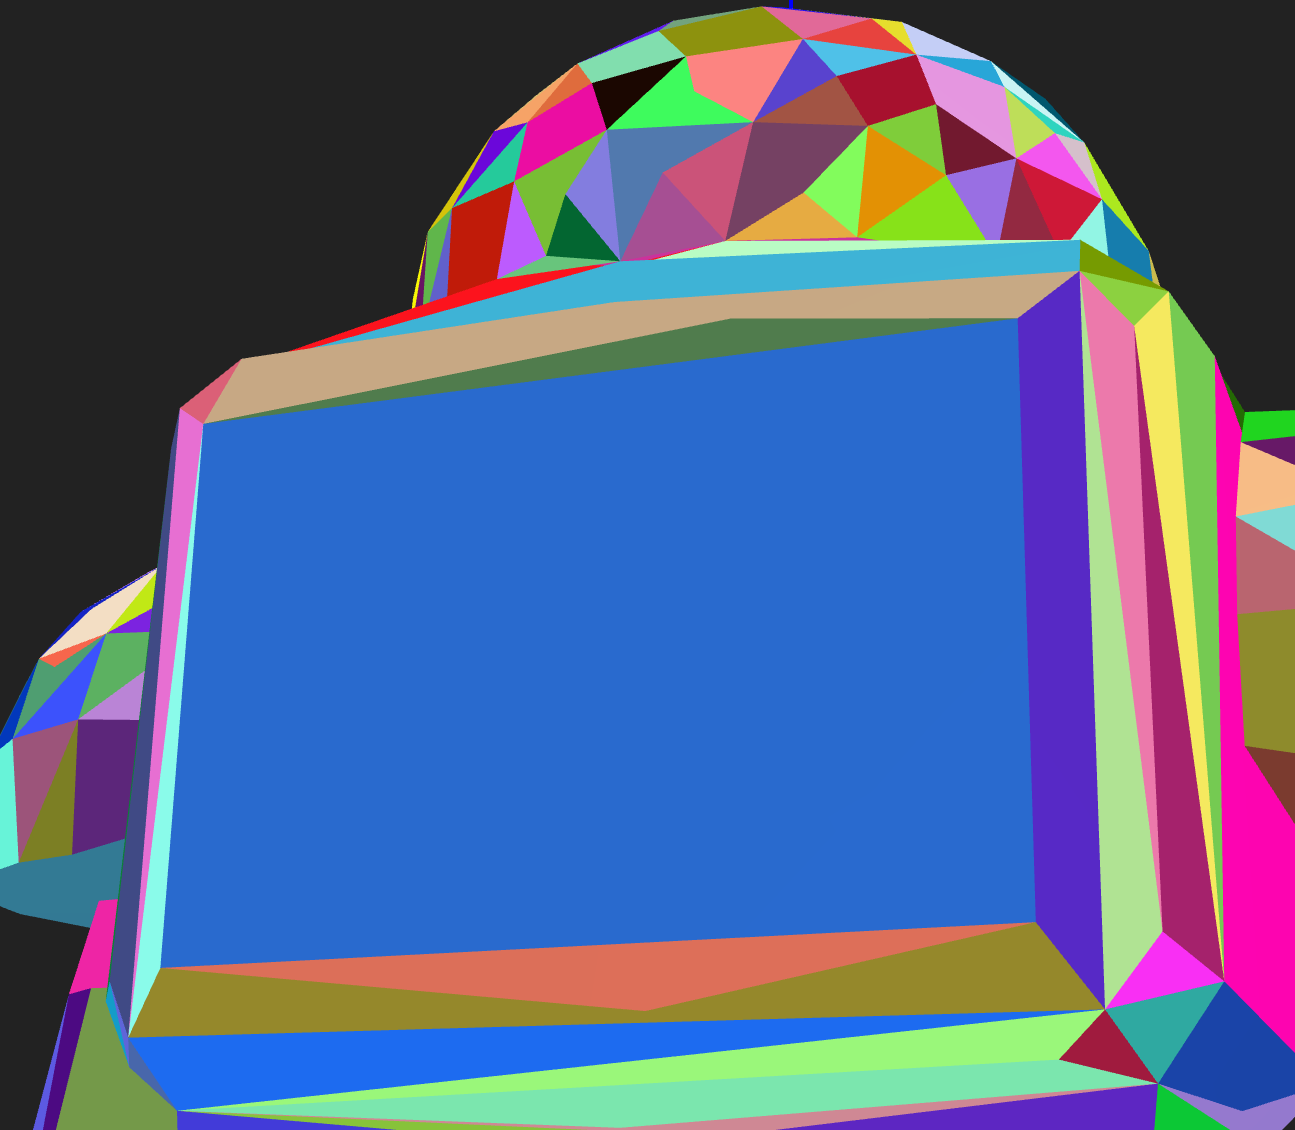
\includegraphics[width=0.8\columnwidth]{Images/04-approx-welding-make-3mm.png}
\caption{Simplified Makerbot with welding distance 3mm - letters completely removed}
\label{fig:3mmMakerbotMake}
\end{figure}

\begin{figure}
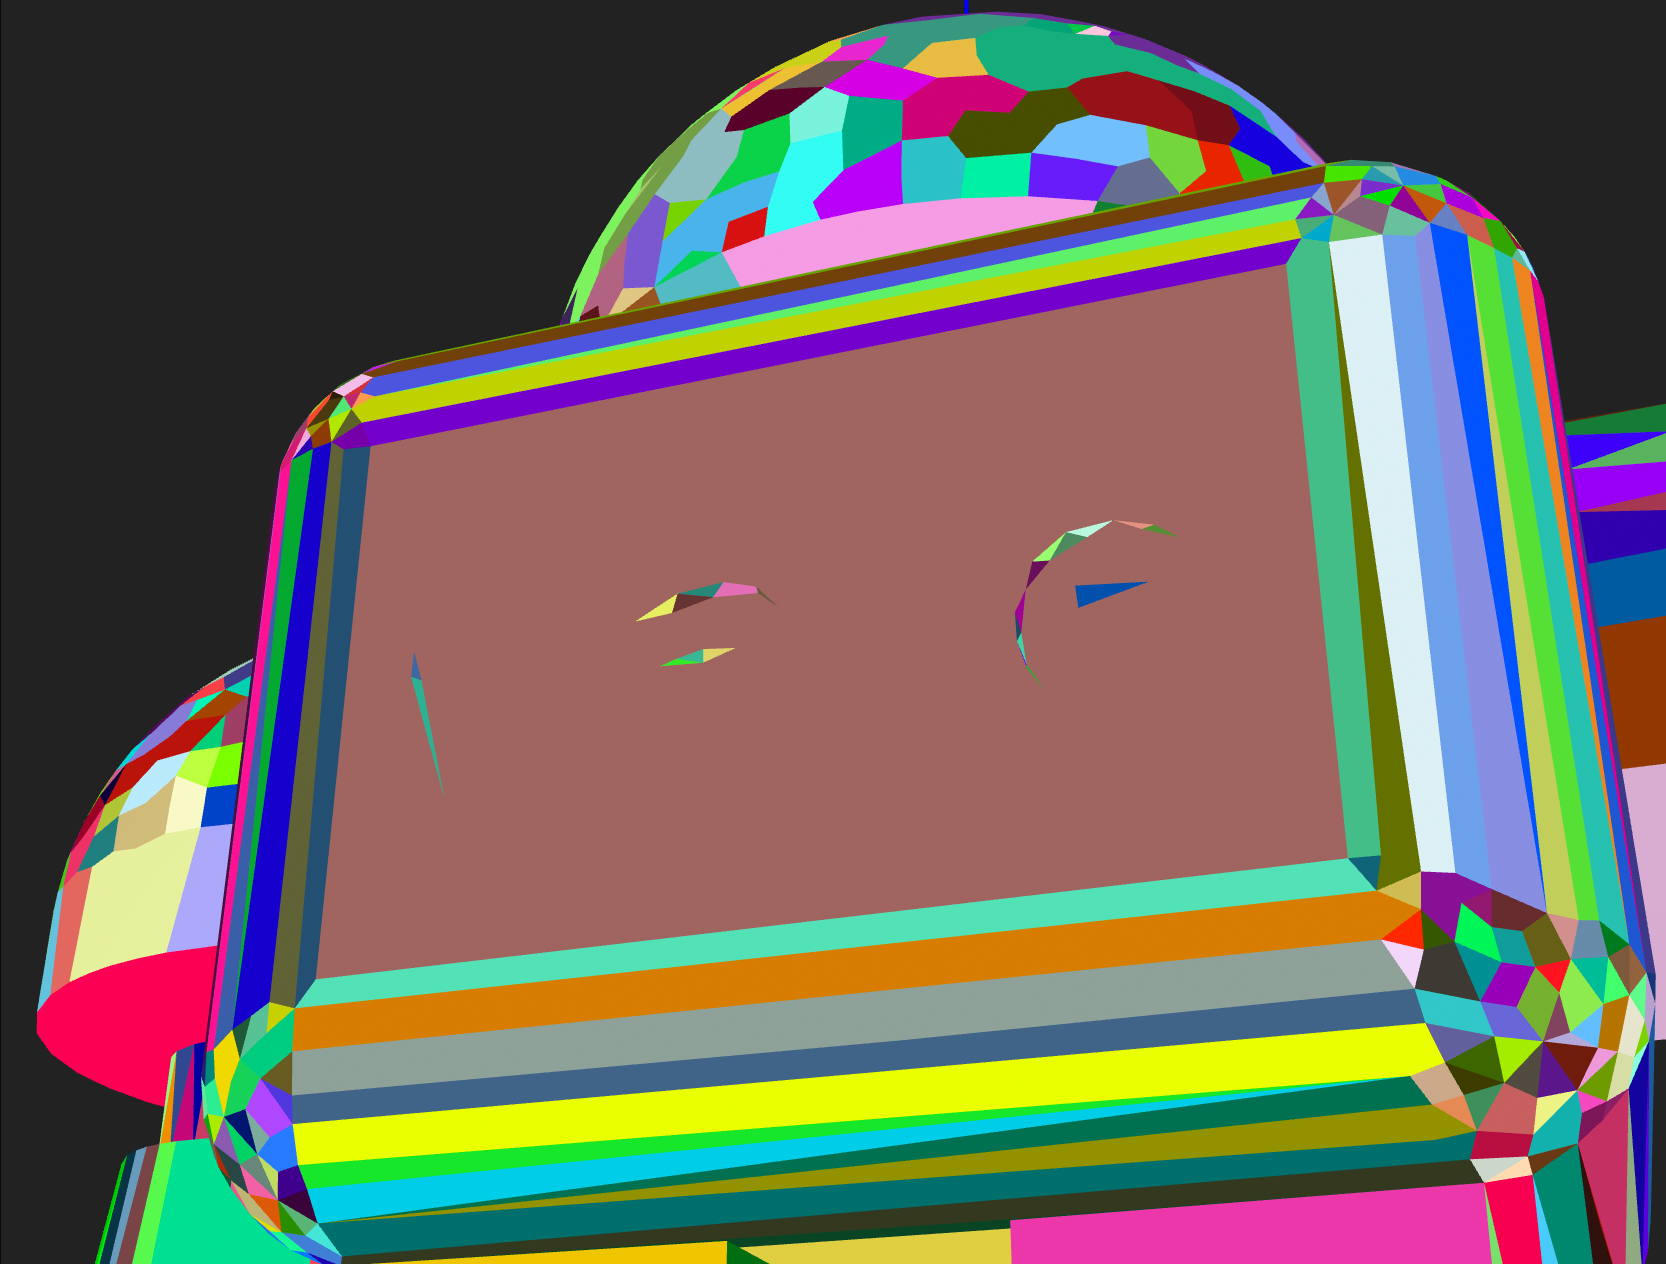
\includegraphics[width=0.8\columnwidth]{Images/04-approx-welding-make-0_8mm.png}
\caption{Simplified Makerbot with welding distance 0.8mm - artifacts}
\label{fig:08mmMakerbotMake}
\end{figure}

\subsubsection{Unwanted Details}

Most 3D editors offer to prettify objects by using curvatures instead of sharp edges. This can be done in various nuances to determine the smoothness of the curve.

Obviously it is much easier to reproduce two connected plates without a beveled edge in \myNotes{InherentPlates (richtiger Name einzusetzen)}. Since these curvatures are just for aesthetic reasons we revert the rounding without any loss of functionality.

Figure \ref{fig:beveled} shows three beveled cubes where the edge is subdivided into one, two and ten parts. All three result in the cube with straight edges after the \emph{Simplification}. The granularity of the created beveled edge does not make any difference for the outcome:
The higher the number of parts the denser the vertices while the absolute distance between start and end of a beveled edge remains the same. Therefore all vertices in this area get merged to the desired point independently from the edge segmentation.

In addition all sorts of surface modification like engravings and small attachments get removed which simplifies the plate recognition. In Figure \ref{fig:extruded_details} there is text on top of the actual surface and in Figure \ref{fig:pushed_in_details} there is text pushed into the surface while both text is removed in the resulting object.


\begin{figure}
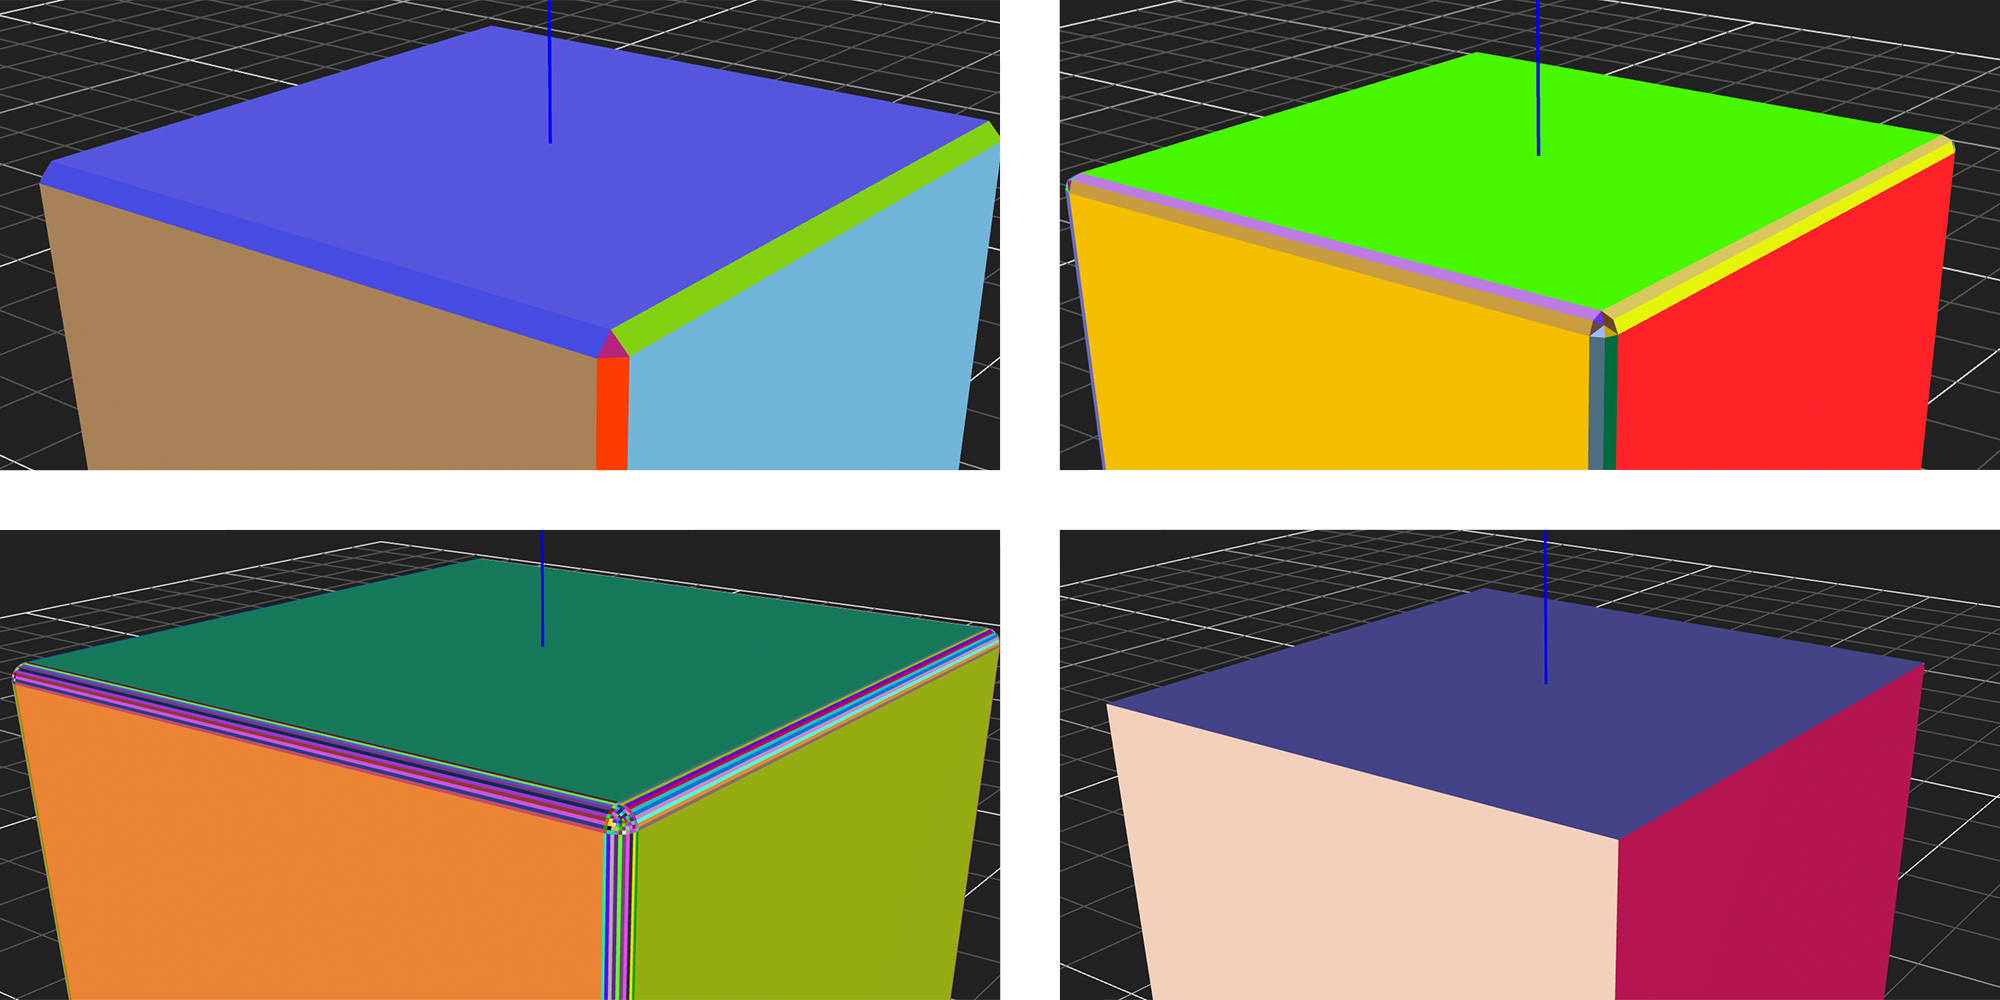
\includegraphics[width=1.0\columnwidth]{Images/04-approx-welding-beveled.png}
\caption{Beveled cube with 1, 2, 10 subdivisions and their resulting cube without beveled edges}
\label{fig:beveled}
\end{figure}

\begin{figure}
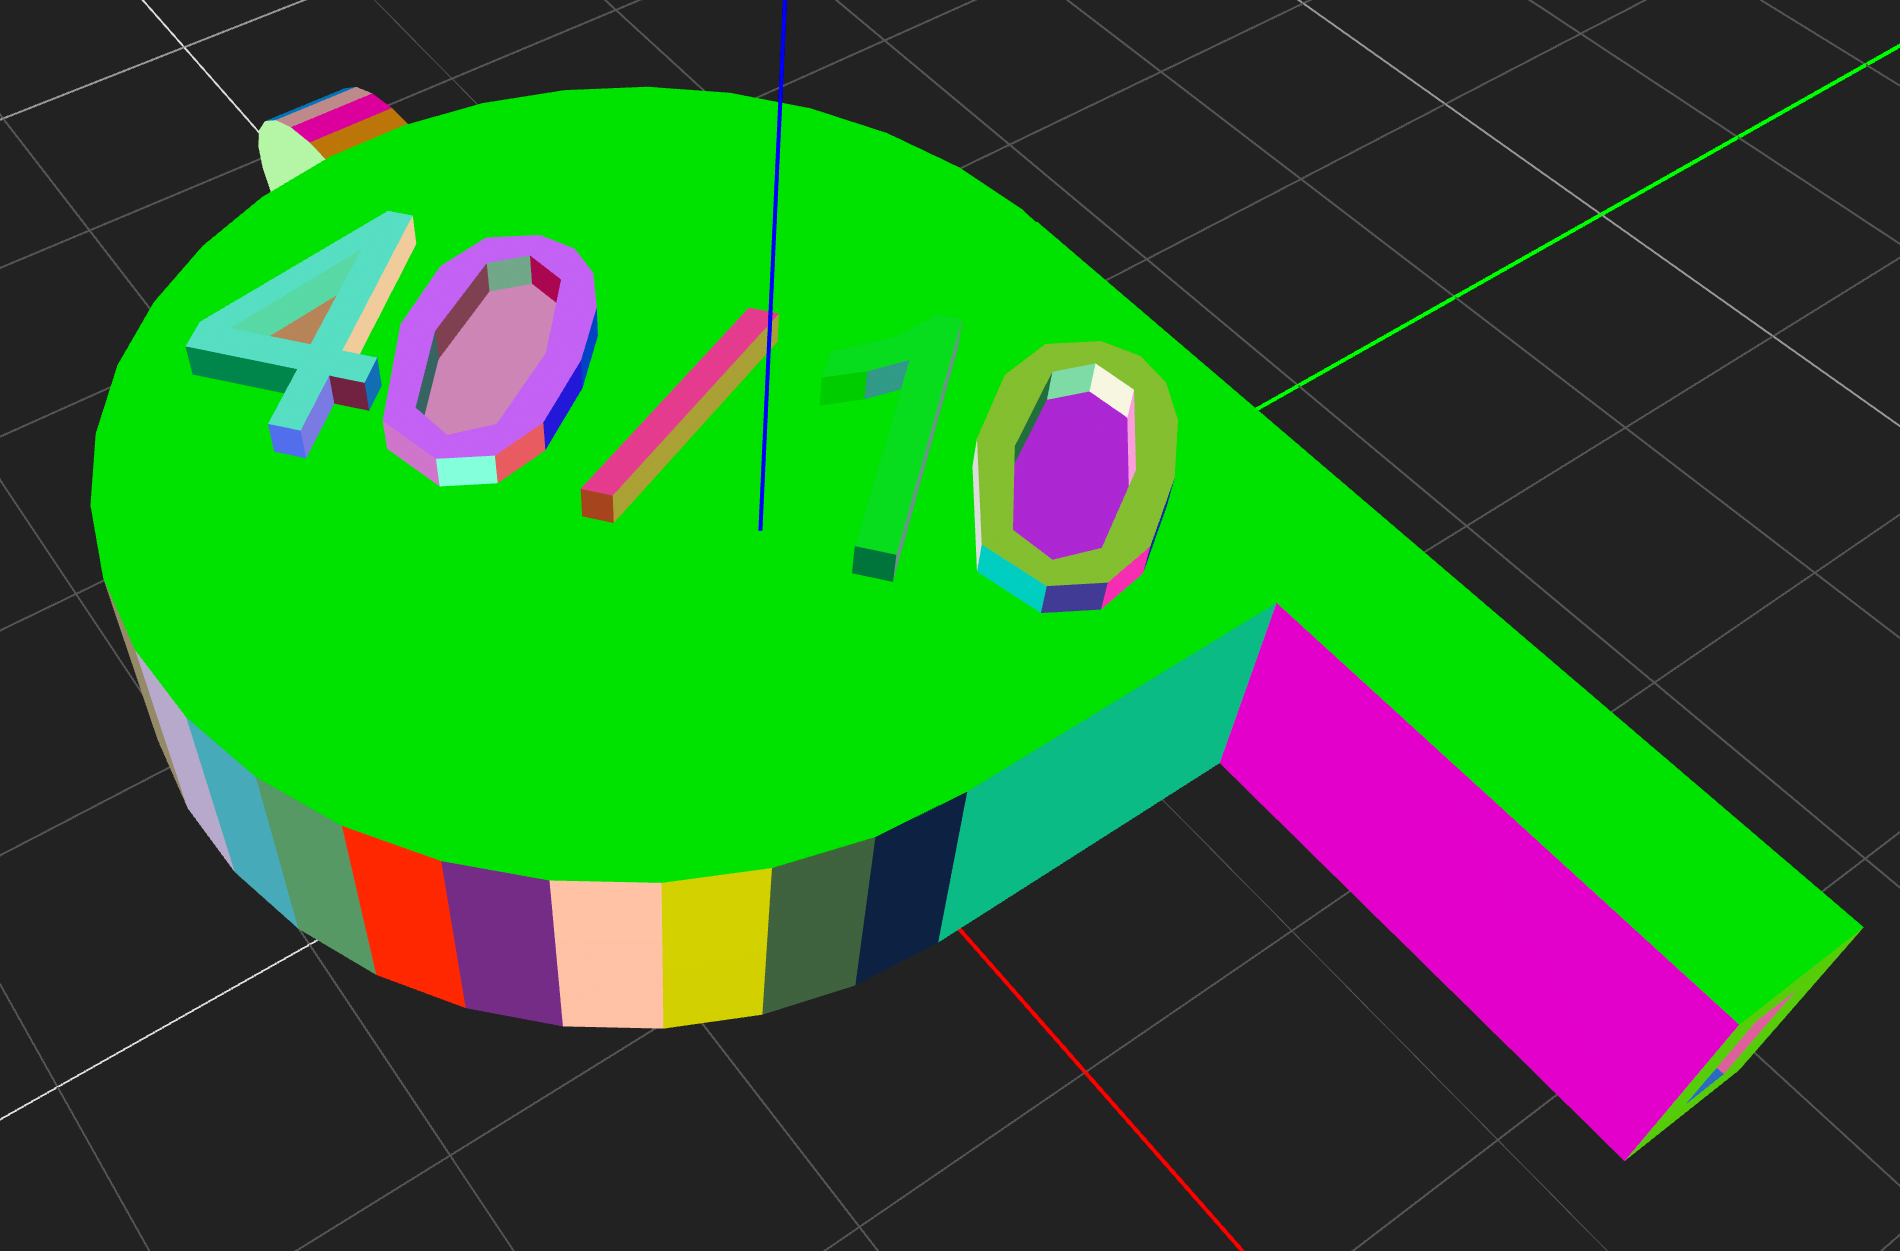
\includegraphics[width=0.5\columnwidth]{Images/04-approx-welding-beveled-extruded.png}
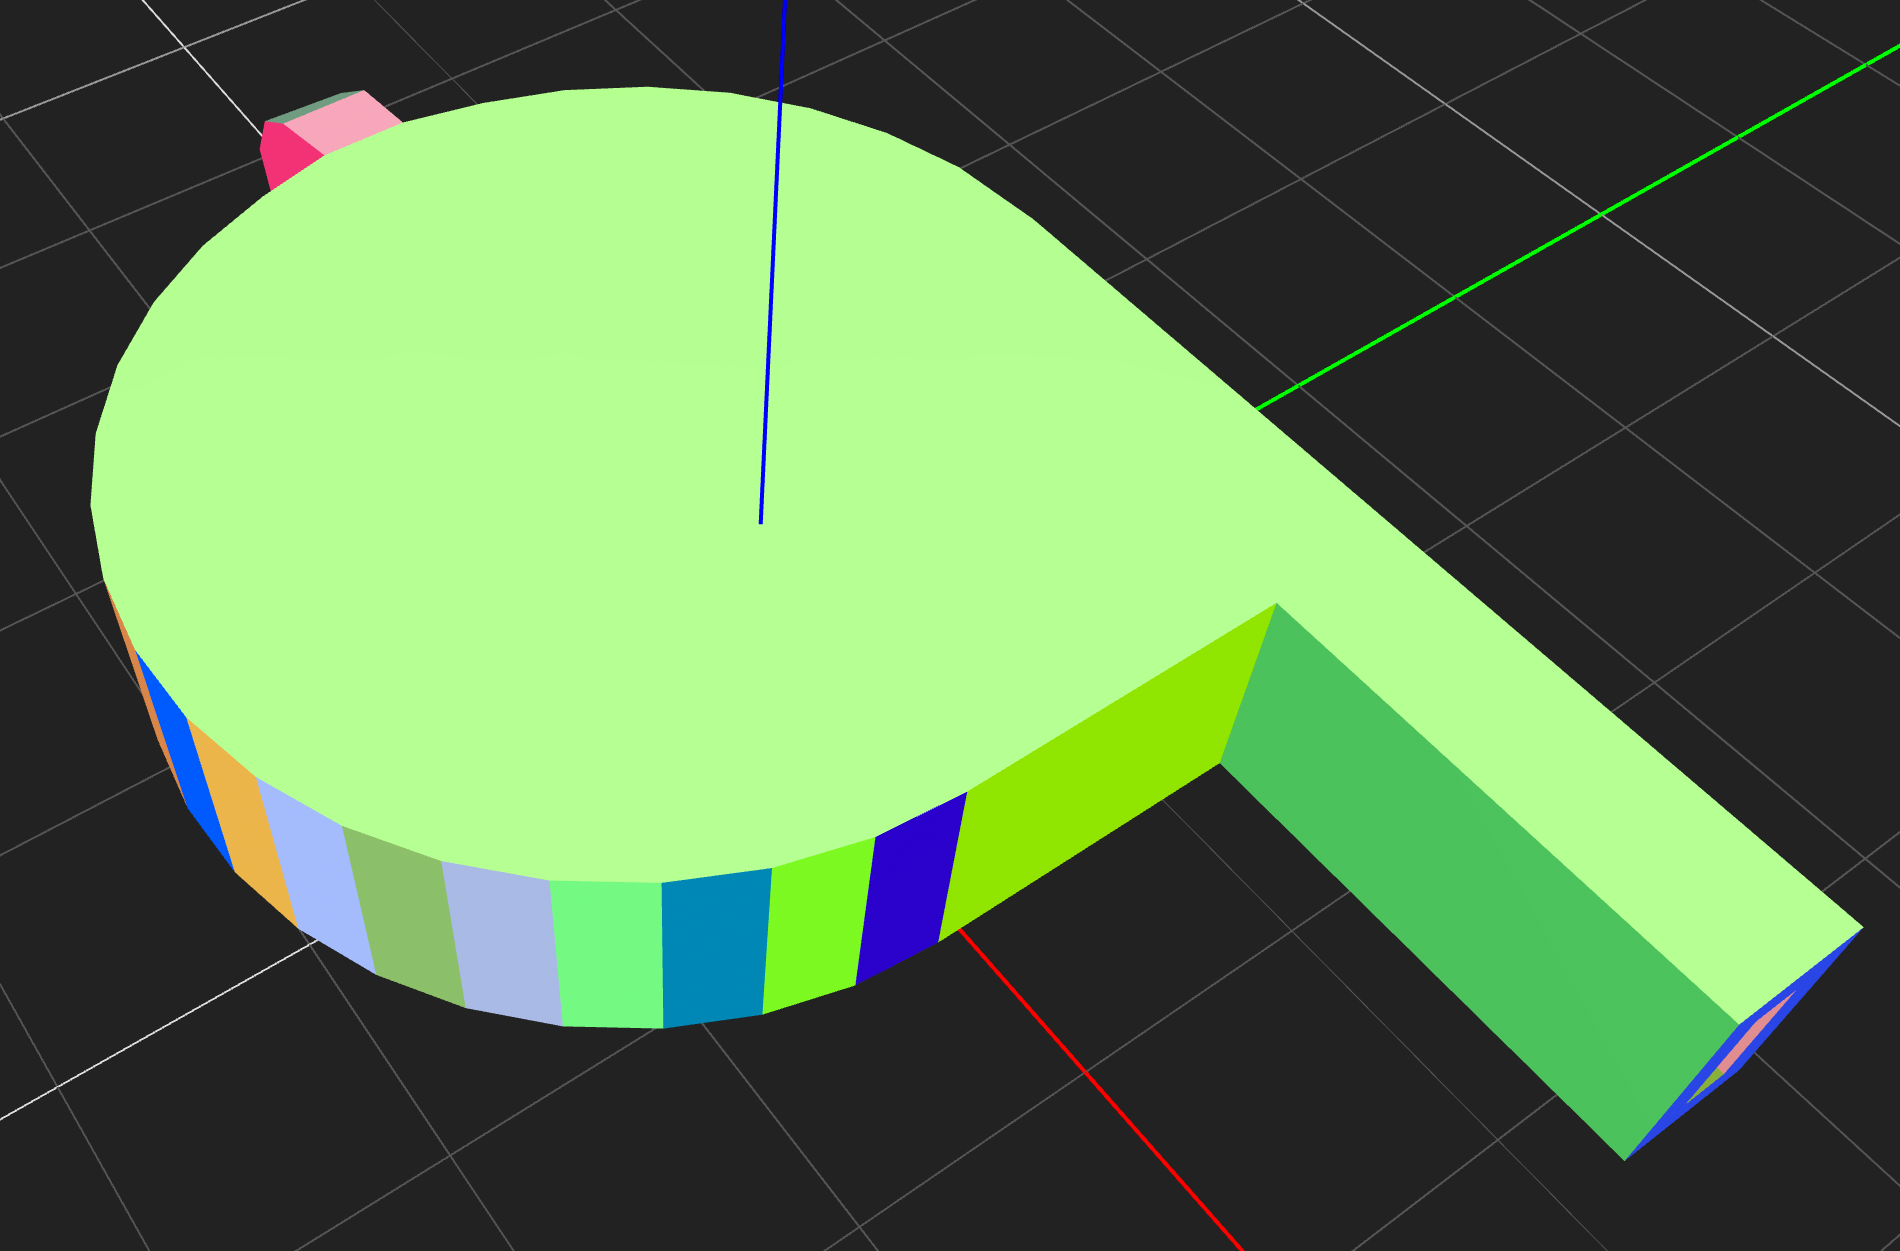
\includegraphics[width=0.5\columnwidth]{Images/04-approx-welding-beveled-extruded-result.png}
\caption{Extruded details}
\label{fig:extruded_details}
\end{figure}

\begin{figure}
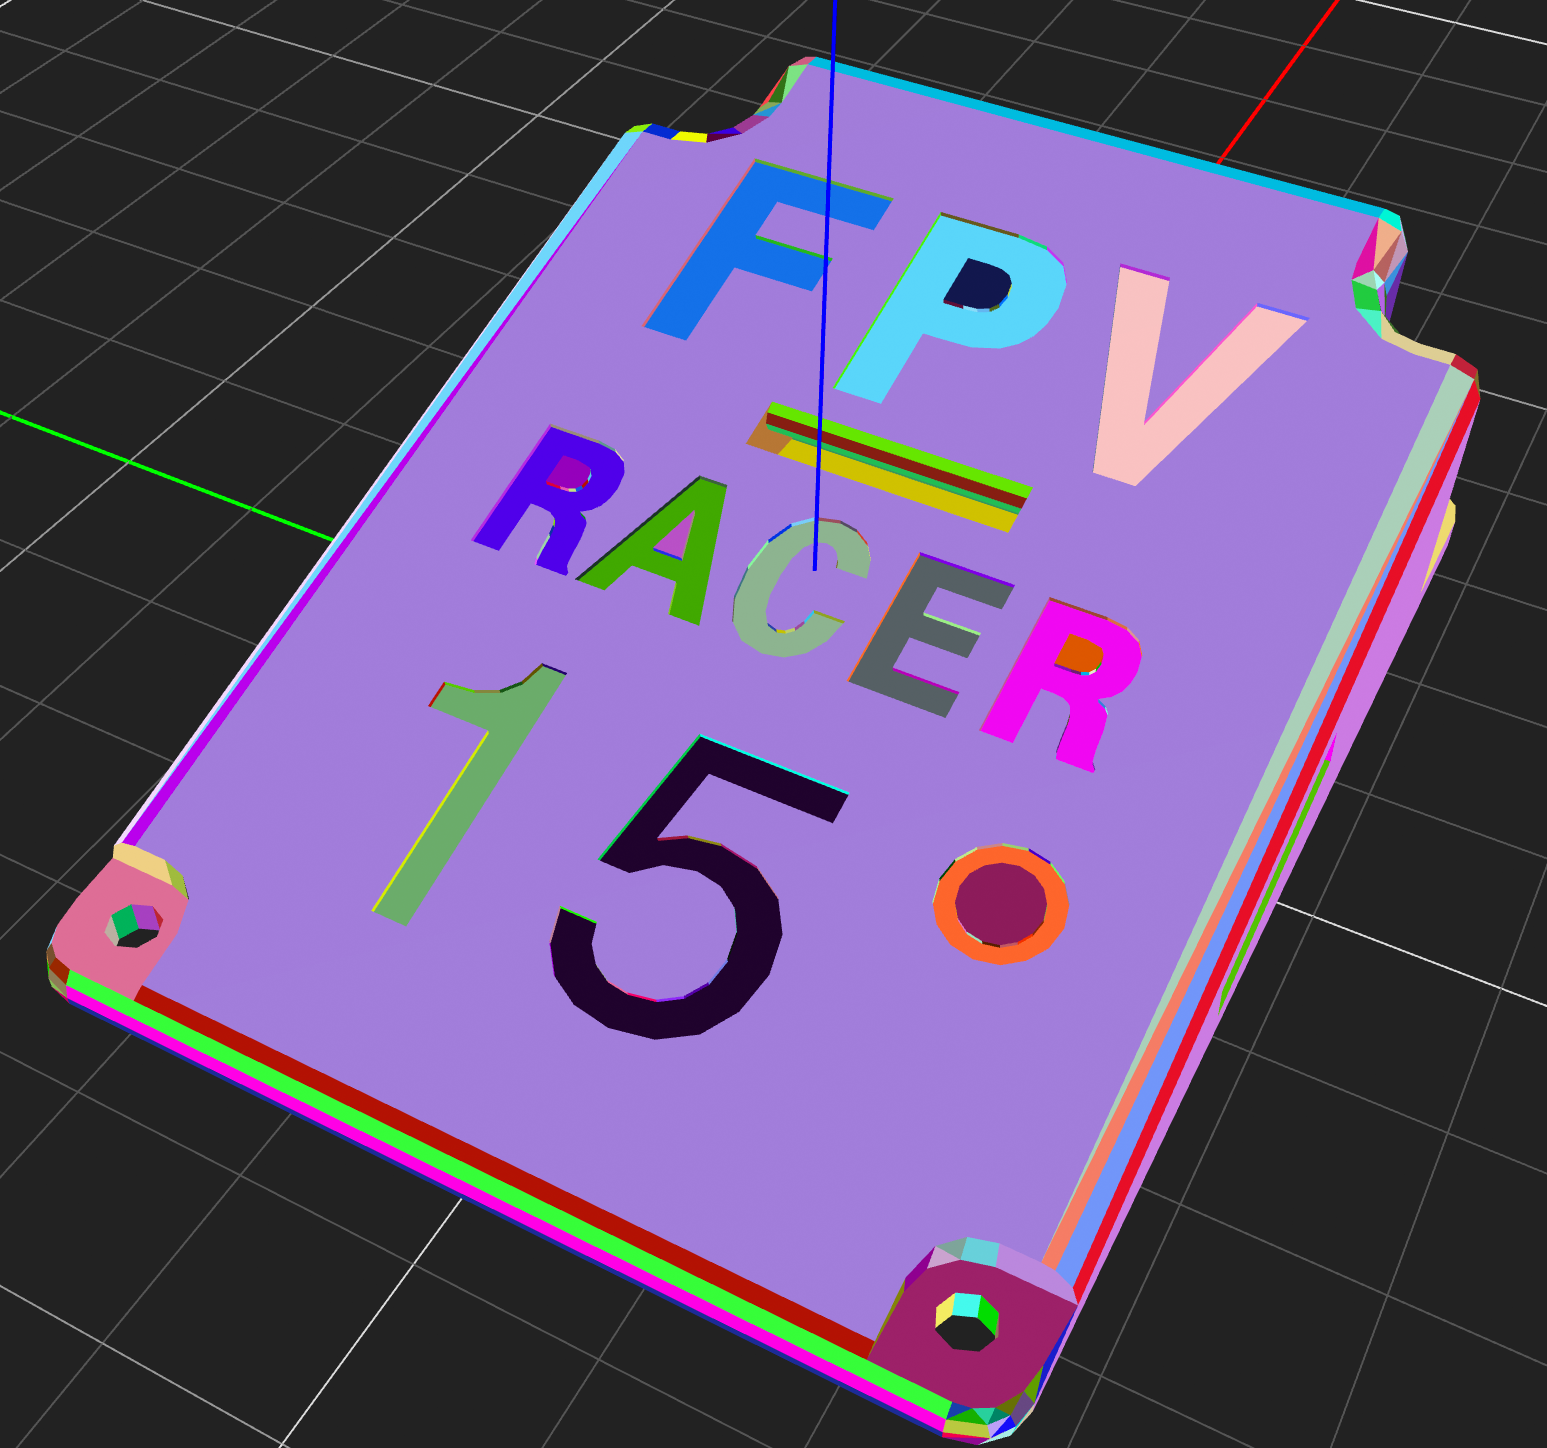
\includegraphics[width=0.5\columnwidth]{Images/04-approx-welding-pushedIn.png}
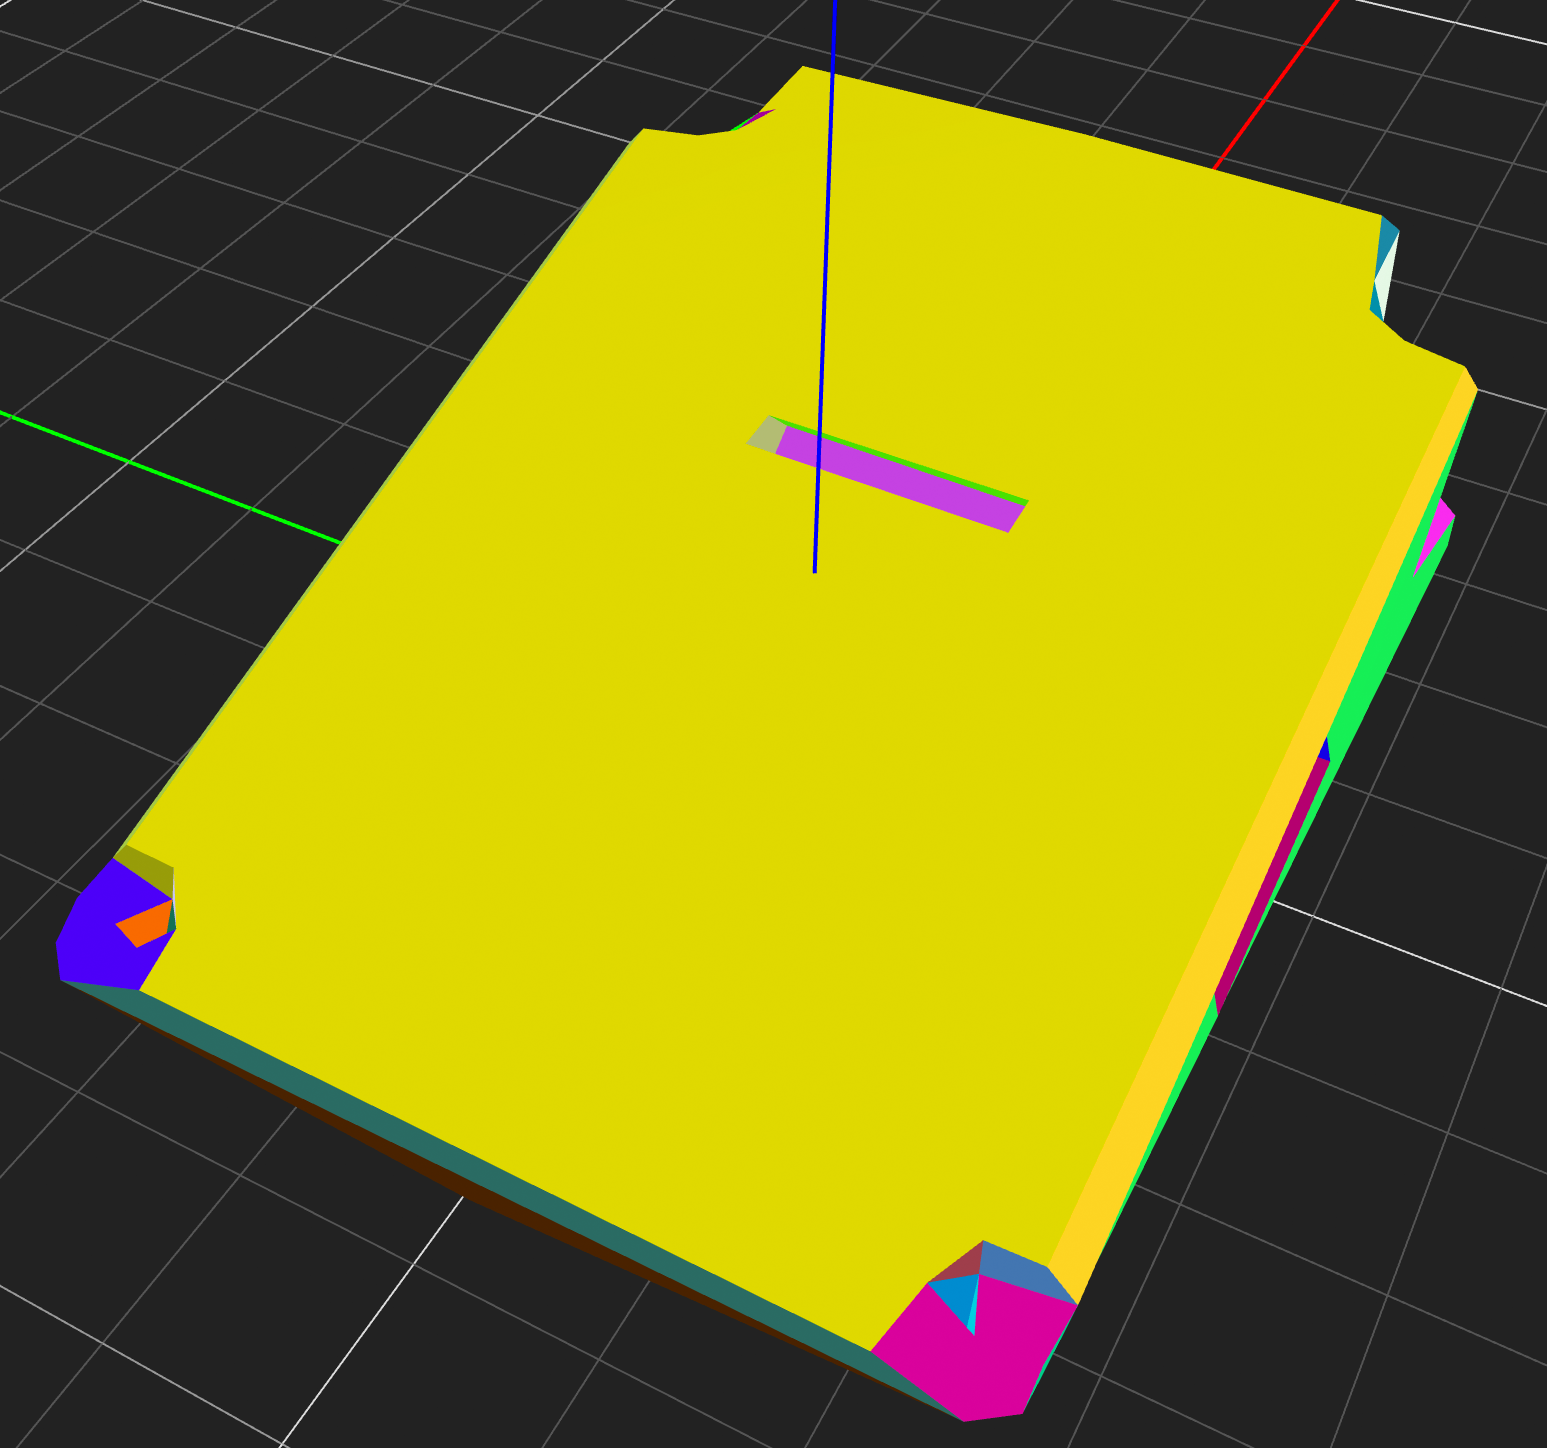
\includegraphics[width=0.5\columnwidth]{Images/04-approx-welding-pushedIn-result.png}
\caption{Pushed in details}
\label{fig:pushed_in_details}
\end{figure}


\subsubsection{Process}

The pipeline step clones the model due to our immutable state approach so the original model can be accessed at any point in time. The immutable state approach is described in chapter \ref{ch:Architecture} Architecture.


\paragraph{Welding Distance}

The welding distance is calculated based on the dimensions of the {\threedmodel}. Very small objects will not be welded at all and the welding distance increases with bigger models.

For most models a welding distance of 2mm is applied which removes all beveled edges created by common editors like Blender\footnote{https://www.blender.org}. Due to the nature of beveled edges all beveling methods only modify small areas around corners which results in dense vertices that get merged by our vertex welding.

The user can modify the welding distance in the UI element shown in Figure \ref{fig:weldingUI}. This is useful if the user only needs a rough approximation and does not care about small details so a greater welding distance can be chosen.

\begin{figure}
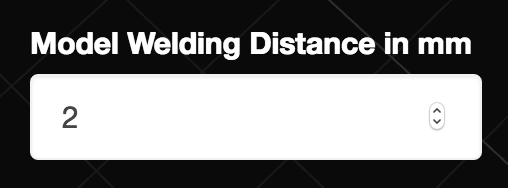
\includegraphics[width=0.5\columnwidth]{Images/04-approx-weldingUI.png}
\caption{Vertex Welding UI Element}
\label{fig:weldingUI}
\end{figure}



\paragraph{Welding}

At first all vertices get preprocessed by the welding algorithm to create the vertex lookup-table. After that the model is passed to \emph{VertexWelding} which iterates over all faces to replace its vertices with their corresponding vertex from the preprocessed table. Meanwhile it checks for invalid faces and deletes them.

\paragraph{Provided Model}

After the actual vertex welding the {\threedmodel} is checked for an empty face set which might occur if the user picked a large welding distance. In this case the stored and unmodified mesh is returned in order to run the rest of the pipeline. The user gets reminded to pick a better welding distance.

The mesh preparation itself is extracted into another pipeline step: \emph{MeshSetup}. It takes the simplified {\threedmodel} and makes it ready for all further processing: face vertex mesh building, normal calculation and mesh indexing.



\subsection{Reusage for redundant information elimination}

The algorithm can be reused in later processing steps. This is done for two reasons:

First a cluster of multiple points lying close together might not bring any additional usable information. So one single representative point of that cluster leads to the same result produced by our system. Therefore the data set can be simplified to improve its processing.

Second a set of points that were only one point in the first place. Different operations on a single vertex shared by multiple primitives lead to slightly different resulting vertices in each primitive. This happens because of floating point inaccuracies. Since these were actually just one point they get merged with our vertex welding.

For instance, this may occur during curve creation as described in chapter \ref{ch:curves} Curves where \emph{VertexWelder} is used to eliminate these point cluster. In general whenever a new data object is generated welding can be applied to ensure unambiguous points.





\subsection{Alternative Methods for Vertex Welding}

There are different ways of implementing vertex welding. The three other appropiate approaches are sorting vertices with an octree, via hashing or via binary space partitioning.

We chose our approach because it serves the simplification step with welding the complete {\threedmodel} as well as reusing it in later processing steps whenever we want to weld a data set. Therefore we do not have to implement different welding methods for various usages. Other implementations may not be applicable, may not serve all usages or will not bring any significant time improvement.

However, the welding can be split into different methods in future work if a runtime improvement is needed. Concretely the pipeline step \emph{simplification} will use an octree to speed up the model simplification and the remaining welding operations will be done with the current implementation.

\paragraph{Octree}

The space is discretised into blocks which dimensions equal the welding distance. At first all vertices are sort into these buckets. Then points are compared within each block along with its 26 surrounding ones and merged accordingly.

This would perform slightly faster for complete mesh simplification and slightly slower for fragmental welding of small vertex sets. Due to the vertex arrangement of most objects the number of comparisons would be lower and consequential the runtime too. On the opposite it performs slower for welding steps that take only a small amount of vertices: Most of them have to be compared so the space discretisation does not bring any advantages.

The implementation of a octree based welding is a bit more complex than the current implementation. We did not chose the octree variant since the current implementation runs in adequate runtime, was faster to code and easier to test.

\paragraph{Hashing}

Hashing is similar to the Octree approach and sorts vertices into a hash list. The sorting is based on a hash value computed by a hash function. This method is usually used if only identical points are merged instead of vertices that lie close to each other.

Due to the nature of hash functions it is easy to identify identical points since they have the same hash vale. Contrary, different points will not end up with the same hash value even if they should be welded in case we use a higher welding distance. Therefore hashing is not applicable to our system.

\paragraph{binary space partition}

Binary space partitioning discretises the space into parts similiar to an octree. It divides the space into unequal parts containing just one point instead of dividing the space into equal parts containing various number of points. Therefore the amount of point comparisons can be reduced which leads to a faster algorithm.

However, the runtime improvement is marginal compared to an octree and is more complicated to implement, test and maintain. Therefore binary space partitioning is not appropiate for our system.





\section{Point on Line Removal}

\emph{PointOnLineRemover} is used by the \emph{ShapesFinder} to delete unnecessary vertices and therefore reducing their complexity. It checks every \emph{EdgeLoop} of a found shape for vertices that lie on implicit lines given by other vertices as shown in figure \myNotes{figure einzusetzen}: Point 2 lies on the line between point 1 and 3 and gets deleted.

\myNotes{TODO: figure}

\emph{Shapes} may represent only a line or a point instead of an 2D-shape if they do not contain enough vertices. An \emph{EdgeLoop} gets deleted if it contains less than three vertices after point on line removal because it does not span an area any more. In case the contour of a \emph{shape} gets deleted the complete \emph{shape} is obsolete and gets deleted as well.

A threshold for the distance of a point to a line is given by the global config since minor deviations from the line are not relevant.

A simplified pseudo code version of the actual removal algorithm is shown in listing \ref{lst:pointOnLineRemovalAlgo}: \emph{getPreviousIndices()} returns the two previous indices that are not removed and \emph{isPreviousOnLine(index, prev, prevprev)} returns true if $ vertex_{prev}$ lies on the line between $vertex_{index}$ and $vertex_{prevprev}$. So we iterate over all vertices while deleting all its previous vertices until the previous is not on the line.

\begin{listing}[!h]
\centering
\begin{minted}[
linenos, breaklines
]{coffeescript}
for index in [0...vertices.length] when index not in removedIndices
    while true
        {prev, prevprev} = @getPreviousIndices(index)
        if @isPreviousOnLine(index, prev, prevprev)
            removedIndices.push(prev)
        else
            break
\end{minted}
\caption{Simplified point on line removal algorithm}
\label{lst:pointOnLineRemovalAlgo}
\end{listing}


When checking if a point lies on a line it is not sufficient to calculate the distance only as illustrated in figure \myNotes{figure einzusetzen}: Point 1 gets deleted in case point 2 lies within threshold distance to the line between point 0 and 1. But the actual point that should be deleted is obviously point 2 since it lies directly on the line between point 1 and 3.

Therefore it is needed to check if a point lies in between the points spanning the line and not outside. In figure \myNotes{figure einzusetzen} point 1 lies outside of the line between point 0 and 2. With this additional check the resulting triangle consist of the points 0, 1 and 3 as obviously desired.

\myNotes{TODO: figure}









\section{Remove Contained Plates - in Lukas Kapitel}
% \secauthor{DS}

\emph{RemoveContainedPlates} is executed after plate generation and removes unnecessary ones that appear with our software.

There are two types of plates that get deleted: First as already described in the master thesis \emph{Platener} \cite{master-thesis} in section '4.4.4 Removing contained plates', small plates can be created that completely lie inside another plate. Second there may be parallel plates that lie inside each other. That occurs due to extrusion if the the 3D object is modeled with thicker blocks than the available material thickness.

We iterate over all plates and compare them to all other plates. The comparison is based on their normals while further checks are not necessary most of the time because the normal check excludes most of them. Therefore the comparison is fast enough and the amount of comparisons must not be reduced with a different iteration algorithm.

\subsection{Plate completely inside another}

As described in the master thesis the algorithm may produce small plates that lie completely inside the actual modeled plate. These plates are orthogonal.

So if two plates have orthogonal normals we check if one of them lies completely in the other and remove it.


\subsection{Overlapping parallel plates}

A 3D block can not be represented by one single plate if it is thicker than a plate. The software creates two plates instead. The resulting plates will overlap in case this block is thinner than those two plates together.

So if two plates are parallel we compare their plane constants which specify the distance to the origin. In case the plane constants hint at overlap the actual \emph{EdgeLoops} are compared to identify intersections. In case they overlap one of the plates gets deleted.










\section{Hole Detection - in Plates Kapitel}
% \secauthor{DS}

The pipeline step \emph{HoleDetection} is run after \emph{ShapesFinder} and categorises every \emph{edgeLoop} of each \emph{shape} either as outer contour or as hole. This is done by computing their areas and comparing them: The \emph{edgeLoop} with the biggest area is the outer contour and all others are holes.












\chapter{Classifiers}
\section{primitives}
\subsection{Prism - Dimitri}
% \secauthor{DS}

\myNotes{Diese subsection wird im Classifier-Kapitel eingefügt}


A Prism is a base element for many other primitives which are characterized by two parallel shapes. Therefore a prism datastructure contains two shapes and the lateral surface as a set of primitives (usually faces or shapes).

To find the prisms all shapes have to be checked for parallelism. The comparison is based on normals which are sorted into buckets to speed up the process. The attached lateral surface can be identified by flood fill.

\subsubsection{Bucket System}
\label{sec:PrismBucketSystem}

The surface normals $\vec{n}$ are sorted into buckets to reduce the amount of comparisons. Treating slightly different normals as equal considering a given threshold $\phi$ each bucket covers this angle. Therefore to check for similarity only normals within a bucket and the surounding ones have to be considered: The angle between two normals is always greater $\phi$ if their buckets are not neighbors. The corresponding bucket for a normal is determined by two values $\alpha$ and $\beta$. Their whose calculation is explained below.

\begin{equation*}
    \vec{n} = \colvec{3}{x}{y}{z}
\end{equation*}


All normals lie on the surface of the unit sphere because of their normalisation. Considering opposite normals as equal (planes with $(1,0,0)$ and $(-1,0,0)$ normals are parallel), all normals are transformed into a hemisphere as shown in Listing \ref{lst:_normalInHemisphere}: A normal is negated in case its $z$ value is negative.


\begin{listing}[!h]
\centering
\begin{minted}[
linenos
]{coffeescript}
_normalInHemisphere: (normal) ->
    if normal.z < 0
        return normal.clone().negate()
    else
        return normal
\end{minted}
\caption{Normals are transformed into hemisphere}
\label{lst:_normalInHemisphere}
\end{listing}

\begin{figure}
    \includegraphics[width=0.7\columnwidth]{Images/PrismCl-Rings.png}
    \caption{rings_FromSide}
    \label{fig:rings_FromSide}
\end{figure}

\begin{figure}
    \includegraphics[width=0.7\columnwidth]{Images/PrismCl-RingsFromTop.png}
    \caption{rings_FromTop}
    \label{fig:rings_FromTop}
\end{figure}

\begin{figure}
    \includegraphics[width=0.4\columnwidth]{Images/PrismCl-RingAngle.png}
    \caption{ringAngle}
    \label{fig:ringAngle}
\end{figure}


This hemisphere is separated into rings. Each ring covers the threshold angle $\phi$ in $z$-direction and is visualized in Figure \ref{fig:rings_FromSide} and Figure \ref{fig:rings_FromTop}. Each normal is sorted into a ring by its correlating angle $\alpha$ which is used to determine the ring index. It is proporional to its coordinates as demonstraded in Figure \ref{fig:ringAngle}: the angle between $\vec{n}$ and $(x,y,0)$:

\begin{equation*}
\begin{split}
    \sin{\alpha} & = \frac{z}{ \sqrt{x^{2} + y^{2}} } \\
    => \alpha  & = \arcsin{ \frac{z}{ \sqrt{x^{2} + y^{2}} } }
\end{split}
\end{equation*}


The angle $\alpha$ is represented as a multiple of the threshold angle $\phi$ to get the actual ring index $I_{Ring}$:

\begin{equation*}
    I_{Ring} = \floor*{
                    \arcsin{
                        \frac{z}{ \sqrt{ x^{2} + y^{2} } }
                    }
                    / \phi
                }
\end{equation*}

The maximum angle is 90° (normal $ = (0,0,1)$). Consequently the maximum ring index $I_{MaxRing}$ is calculated as follows:

\begin{equation*}
    I_{MaxRing} = \floor*{
                    \frac{\pi}{2}
                    / \phi
                  }
\end{equation*}



The angle in the middle of each ring ${\alpha}_{I_{Ring}}$ consequently depends on index and threshold:

\begin{equation}
\label{equ:AlphaIRing}
    {\alpha}_{I_{Ring}} = (I_{Ring} + 0.5) * \phi \qquad \forall{ I_{Ring} \in [0, I_{MaxRing}] }
\end{equation}



Figure \ref{fig:middleZ} implies the calculation of the corresponding middle $z$ value $z_{I_{Ring}}$: We create a normal $\vec{a}_{I_{Ring}}$ with a fixed $y$ value of 0 that forms the angle ${\alpha}_{I_{Ring}}$ with the unit vector in x direction $\vec{v}_{x}$. Consequently all normals that lie in the middle of a ring ($\alpha = {\alpha}_{I_{Ring}}$) have the $z$ value $z_{I_{Ring}}$.

\begin{figure}
    \includegraphics[width=0.5\columnwidth]{Images/PrismCl-MiddleZ.png}
    \caption{middleZ}
    \label{fig:middleZ}
\end{figure}

\begin{equation}
\label{equ:VecX}
    \vec{v}_{x} = (1, 0, 0)
\end{equation}

\begin{equation}
\begin{split}
    \label{equ:VecA}
    \vec{a}_{I_{Ring}} = (x_{a}, 0, z_{I_{Ring}}) \qquad  & \forall{ I_{Ring} \in [0, I_{MaxRing}] } \\
    & with \vert \vec{a}_{I_{Ring}} \vert = 1
\end{split}
\end{equation}

\begin{equation}
    \label{equ:XA}
    \cos{{\alpha}_{I_{Ring}}} = \frac{ \vec{v}_{x} * \vec{a}_{I_{Ring}} }{ \vert \vec{v}_{x} \vert * \vert \vec{a}_{I_{Ring}} \vert }
    \stackrel{(\ref{equ:VecX}) + (\ref{equ:VecA})}{=} \vec{v}_{x} * \vec{a}_{I_{Ring}}
    \stackrel{(\ref{equ:VecX}) + (\ref{equ:VecA})}{=} x_{a}
\end{equation}

\begin{equation}
\label{equ:ZIRing}
\begin{split}
    1 & = \vert \vec{a}_{I_{Ring}} \vert \stackrel{(\ref{equ:VecA})}{=} \sqrt{ x_{a}^{2} + z_{I_{Ring}}^{2} } \\
    => z_{I_{Ring}} & = \sqrt{1 - x_{a}^{2}}
    \stackrel{(\ref{equ:XA})}{=} \sqrt{1 - cos^{2}{{\alpha}_{I_{Ring}}}}
\end{split}
\end{equation}


Each ring is seperated into buckets which cover the threshold angle $\phi$ as shown in Figure \ref{fig:PrismCl-buckets}. Therefore the onto the xy-plane projected angle $\gamma$ needs to be calculated which differs from ring to ring. This is shown in Figure \ref{fig:projection} and leads to this calculation:

\begin{figure}
    \includegraphics[width=0.7\columnwidth]{Images/PrismCl-buckets.png}
    \caption{buckets}
    \label{fig:PrismCl-buckets}
\end{figure}


\begin{figure}
    \includegraphics[width=1.0\columnwidth]{Images/PrismCl-Projection.png}
    \caption{projection}
    \label{fig:projection}
\end{figure}


$ \vec{a}_{I_{Ring}}' $ is the projection of $\vec{a}_{I_{Ring}} $:


\begin{equation}
    \label{equ:VecAStrich}
    \vec{a}_{I_{Ring}}' = (x_{a}, 0)
\end{equation}

$ \vec{b}_{I_{Ring}} $ spans the threshold angle $\phi$ with $ \vec{a}_{I_{Ring}} $ and has the same $z$ value $z_{I_{Ring}}$:

\begin{equation}
    \vec{b}_{I_{Ring}} = (x_{b}, y_{b}, z_{I_{Ring}}) \qquad with | \vec{b}_{I_{Ring}}| = 1
    \label{equ:VecB}
\end{equation}

The corresponding projected vector $ \vec{b}_{I_{Ring}}' $:

\begin{equation}
    \vec{b}_{I_{Ring}}' = (x_{b}, y_{b})
    \label{equ:VecBStrich}
\end{equation}

Due to the mentioned conditions the coordinates of $ \vec{b}_{I_{Ring}} $ are calculated as follows:


\begin{equation}
    \label{equ:Projection1}
    \cos{\phi} = \frac{\vec{a}_{I_{Ring}} * \vec{b}_{I_{Ring}}}{|\vec{a}| * |\vec{b}|} = \vec{a}_{I_{Ring}} * \vec{b}_{I_{Ring}} \stackrel{(\ref{equ:VecA}) + (\ref{equ:VecB})}{=} x_{a}_{I_{Ring}} * x_{b}_{I_{Ring}} + z_{I_{Ring}}^{2}
\end{equation}

\begin{equation}
    \label{equ:XB}
   (\ref{equ:Projection1}) => x_{b} = \frac{ \cos{\phi} - z_{I_{Ring}}^{2} }{ x_{a} }
\end{equation}

\begin{equation}
\begin{split}
    \label{equ:YpsilonB}
    & 1 = |\vec{a}_{I_{Ring}}| = |\vec{b}_{I_{Ring}}| \\
    & => \sqrt{ x_{a}^{2} + z_{I_{Ring}}^{2} } = \sqrt{ x_{b}^{2} + y_{b}^{2} + z_{I_{Ring}}^{2} } \\
    & => y_{b} = \sqrt{ x_{a}^{2} - x_{b}^{2} }
\end{split}
\end{equation}


The angle ${\gamma}_{I_{Ring}}$ which is used to separate a ring into buckets is calculated with the projected vectors $ \vec{a}_{I_{Ring}}' $ and $ \vec{b}_{I_{Ring}}' $ :

\begin{equation}
\begin{split}
    \cos{{\gamma}_{I_{Ring}}}& = \frac{\vec{a}_{I_{Ring}}' * \vec{b}_{I_{Ring}}'}{|\vec{a}_{I_{Ring}}'| * |\vec{b}_{I_{Ring}}'|}
    = \frac{ x_{a} * x_{b} }{ x_{a} * \sqrt{  x_{b}^{2} +  y_{b}^{2} } } \\
    & \stackrel{(\ref{equ:YpsilonB})}{=} \frac{ x_{a} * x_{b} }{ x_{a} * \sqrt{  x_{b}^{2} - x_{b}^{2} +  x_{a}^{2} } }
    = \frac{ x_{a} * x_{b} }{ x_{a} * x_{a} }
    = \frac{ x_{b} }{ x_{a} } \\
    & \stackrel{(\ref{equ:XB})}{=} \frac{ \cos{\phi} - z_{I_{Ring}}^{2} }{ x_{a}^{2} }
    \stackrel{(\ref{equ:XA})}{=} \frac{ \cos{\phi} - z_{I_{Ring}}^{2} }{ \cos^{2}{{\alpha}_{I_{Ring}}} } \\
    & \stackrel{(\ref{equ:ZIRing})}{=} \frac{ \cos{\phi} - ( 1 - cos^{2}{{\alpha}_{I_{Ring}}} ) }{ \cos^{2}{{\alpha}_{I_{Ring}}} }
    = \frac{ \cos^{2}{{\alpha}_{I_{Ring}}} }{ \cos^{2}{{\alpha}_{I_{Ring}}} } + \frac{ \cos{\phi} - 1 }{ \cos^{2}{{\alpha}_{I_{Ring}}} } \\
    & \stackrel{(\ref{equ:AlphaIRing})}{=} 1 + \frac{ \cos{\phi} - 1 }{ \cos^{2}{( (I_{Ring} + 0.5) * \phi )} } \\
    => {\gamma}_{I_{Ring}} & = \arccos{( 1 + \frac{ \cos{\phi} - 1 }{ \cos^{2}{( (I_{Ring} + 0.5) * \phi )} } )}
\end{split}
\end{equation}


The corresponding angle $ \beta $ of a normal $ \vec{n} $ is calculated with use of the unit vector in x direction $ \vec{v_{x}'} $. This angle needs to be adapted in case $ y < 0 $ since the maximum angle between two vectors is 180° and we want to cover a complete circle:

\begin{equation}
\begin{split}
    \cos{\beta} & = \frac{\vec{n}' * \vec{v_{x}'}}{|\vec{n}'| * |\vec{v_{x}'}|} = \frac{x}{\sqrt{x^{2} + y^{2}}} \\
    => \beta & = \begin{cases}
        \arccos{ \frac{x}{\sqrt{x^{2} + y^{2}}} }, & y \geq 0 \\
        2 \pi - \arccos{ \frac{x}{\sqrt{x^{2} + y^{2}}} }, & y < 0
    \end{cases}
\end{split}
\end{equation}

The angle $ \beta $ is represented as a multiple of the $ \gamma $ angle to get the bucket index $ I_{Bucket} $:

\begin{equation}
    I_{Bucket} = \floor{\frac{\beta}{ {\gamma}_{I_{Ring}} }}
\end{equation}

Consequently the maximum bucket index is calculated with the maximum angle of 360°:

\begin{equation}
    I_{MaxBucket} = \floor{\frac{2 \pi}{ {\gamma}_{I_{Ring}} }}
\end{equation}



\subsubsection{Implementation}

\myNotes{TODO: Klassendiagramm}

The \emph{PrismClassifier} works on \emph{shapes} from the \emph{ClassifierGraph} and should also take account of \emph{planes} in future development. Therefore it depends on the \emph{PlaneClassifier}. It returns a set of \emph{prisms} and uses \emph{PrismShapeNormalsBuckets} to check shapes for parallelism.

\paragraph{PrismClassifier}

\begin{listing}[!h]
\centering
\begin{minted}[
linenos, breaklines
]{coffeescript}
run: ->
    return new Promise( (resolve) =>
        buckets = new PrismShapeNormalsBuckets(_angleThreshold)

        @_putIntoBuckets @shapes, buckets

        prisms = @_detectPrisms @shapes, buckets

        log.debug("PrismClassifier found " + prisms.length + " prisms")

        resolve(prisms)
    )
\end{minted}
\caption{run method of the PrismClassifier}
\label{lst:PrismClassifierRun}
\end{listing}

Listing \ref{lst:PrismClassifierRun} shows the implementation of the \emph{PrismClassifier} run method:

At first the normal buckets are initialised with an angle threshold as described in section \emph{Bucket System}. These values are stored in the global config with \emph{\_angleThreshold} $ = 0.15 $  ( = 8.6\textdegree, previously labeled $\phi$) so shapes with an angle  of 8.6\textdegree \hspace{1pt} will be considered parallel.

Then all shapes are put into the corresponding buckets. This is done by iterating over all shapes and passing them to the bucket system which handles the classification on its own.

Next we iterate over all shapes again while requesting the potential parallel shapes from the bucket system. The shapes are checked with the given threshold and a \emph{prism} is created in case of parallelism.

At the end a set of all prisms is returned which can be used for further primitive classification.


\paragraph{PrismShapeNormalsBuckets}

\emph{PrismShapeNormalsBuckets} is based on the specification in section \ref{sec:PrismBucketSystem} Bucket System: It divides a hemisphere into rings with buckets and is initialised with the angle threshold.

The constructor saves the angle threshold, instantiates the rings as a \emph{javascript map} and calculates the maximum ring index $I_{MaxRing}$.

It provides two functions used by the classifier: \\
\emph{push} and \emph{getShapesToCheckAndDeleteThisOne}.

\emph{push} takes a \emph{shape} and puts it in the corresponding ring. At first it transforms its normal into the hemisphere. Then the ring index $ I_{Ring} $ is calculated. If the ring is not initialised yet it gets created and \emph{ring.push(shape)} is called to sort the \emph{shape} into the corresponding bucket.

\emph{getShapesToCheckAndDeleteThisOne} takes a shape and removes it from the bucket system because it will be checked for all possible prisms by the classifier and should not be returned as a potential parallel shape in another pass. Then it returns an array of all shapes lying in the same and the surrounding buckets: It requests the corresponding buckets from the ring with the shape's ring index $ I_{Ring} $ and the ring above and beneath.

While determining the surrounding rings following special cases need to be considered:

First: The ring with the maximum index $I_{MaxRing}$ is only adjacent to the ring underneath, because it is the highest ring on top of the hemisphere. It is not separated into different buckets and serves as a single bucket which is adjacent to all buckets in the ring underneath.

Second: The ring with index 0 "is adjacent to itself" because the unit sphere got transformed into a hemisphere. Therefore the buckets 180° around have to be taken into account for parallelism checks. Let's take two normals with the same x, y coordinates and a negated z value that span an angle smaller $ \phi $: $\vec{n_{1}} = (x, y, z)$ and $\vec{n_{2}} = (x, y, -z)$ with $z > 0$. Consequently $\vec{n_{1}}$ naturally lies in ring 0 and $\vec{n_{2}}$ gets negated to fit into the hemisphere. The negated normal is $\vec{n_{2}}' = (-x, -y, z) $ and lies also in ring 0 but in the opposite bucket (180° away).


\paragraph{Ring}

A \emph{Ring} contains buckets as a javascript map and is initialized with an index $ I_{Ring} $ and the angle threshold $ \phi$. With these the angle $ \gamma $ and the maximum bucket index $ I_{MaxBucket} $ are calculated as described in section \ref{sec:PrismBucketSystem} Bucket System. It provides the methods \emph{push}, \emph{get}, \emph{getAndSurrounding}, \emph{getAll}, \emph{delete} and \emph{getSize}

The method \emph{push} sorts a given shape into the corresponding bucket. \emph{get} returns all shapes of a bucket with a given index, \emph{getAndSurrounding} returns the same and additionaly the two neighboring buckets while \emph{getAll} returns all shapes that lie in that ring. With \emph{delete} a given shape is removed from the ring and \emph{getSize} returns the amount of shapes that lie in that ring.


\paragraph{MaxRing} The \emph{MaxRing} is only instanced once and is the ring with index $ I_{RingMax} $. It provides the same methods as a \emph{Ring} but with adapted behaviour.

\paragraph{Prism}

A \emph{Prism} contains two parallel shapes that span a prism. In future work this should be extended by the lateral surface which is not handlet yet.

\subsubsection{Future Work}
\label{sec:PrismFutureWork}

\paragraph{Planes} \emph{Planes} from the \emph{PlaneClassifier} should be taken into account in addition to the shapes. Ideally the \emph{PlaneClassifier} detects noisy planes that are not represented as shapes. Therefore a better approximation of the original model could be achieved.

\paragraph{Lateral Surface} The lateral surface of the prism has yet to be identified and added to the prism structure. This is needed for further operations and more specific classifications of the prism. For example for classifying a cube the surrounding sides have to be known.

\paragraph{Scoring} Prism scoring is not implemented yet. To rate a prism the actual angle between the two nearly parallel shapes have to be considered. If scoring is implemented the angle threshold for parallelism can be adjusted to a much higher value while big variations to 0° will be reflected in the score.


\end{document}

\cleardoublepage

%\part{Plates}
\subfile{Chapters/05-Plates}
%\documentclass[../ClassicThesis.tex]{subfiles}
\begin{document}

%************************************************
\chapter{Plates}\label{ch:plates}
%************************************************

\section{Overview of approaches for finding plates}

There are multiple approaches for finding plates contained in a 3D-mesh. The first, called inherent plates, requires the plates to be modeled in the mesh with both a top and a bottom side (see Figure \ref{fig:inhplates}). The second approach, extruded plates, uses the mesh surface to extrude plates into the object (Figure \ref{fig:extplates}). While this method works on more meshes then the inherent approach, it can produce doubled plates if they are modeled in the mesh. The third approach is to stack plates, creating a filled approximation of the mesh (Figure \ref{fig:staplates}).

\begin{figure}
    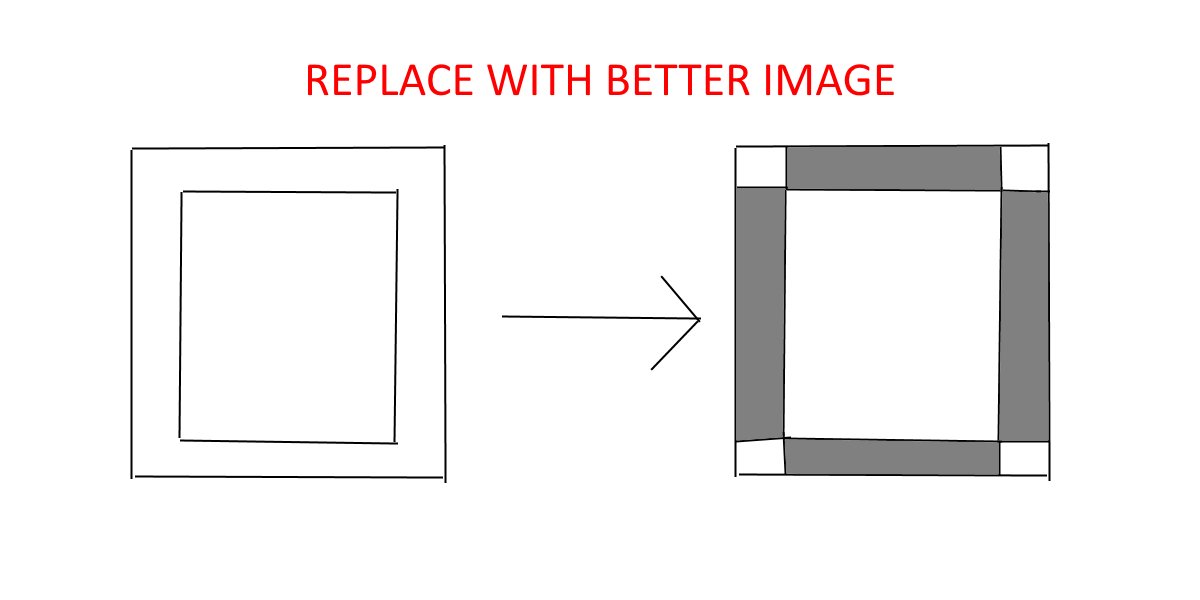
\includegraphics[width=1.0\columnwidth]{Images/plates_inherentplates.png}
    \caption{Finding inherent plates.}
    \label{fig:inhplates}
\end{figure}

\begin{figure}
    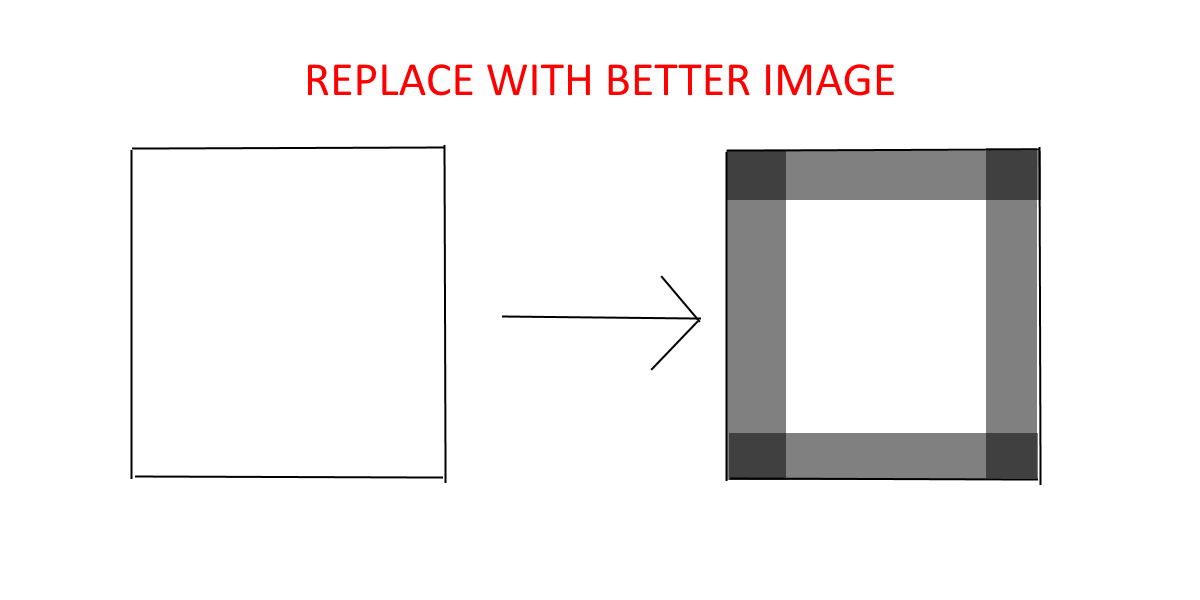
\includegraphics[width=1.0\columnwidth]{Images/plates_extrudedplates.png}
    \caption{Finding extruded plates.}
    \label{fig:extplates}
\end{figure}

\begin{figure}
    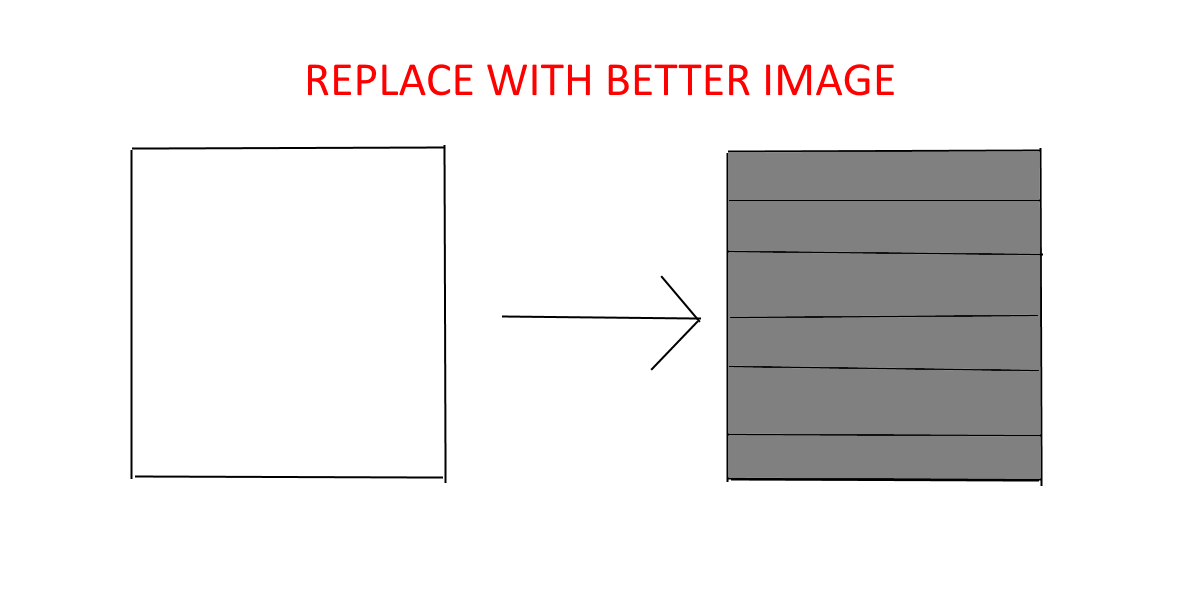
\includegraphics[width=1.0\columnwidth]{Images/plates_stackedplates.png}
    \caption{Finding stacked plates.}
    \label{fig:staplates}
\end{figure}

\section{Prerequisites for finding plates}

Before finding plates, the model's faces have to be grouped into planar surfaces (Figure \ref{fig:coplanar}). This is done by checking the angle between adjacent faces. Afterwards, the resulting shapes' edge loops are generated and the contour is differentiated from the holes.

\begin{figure}
    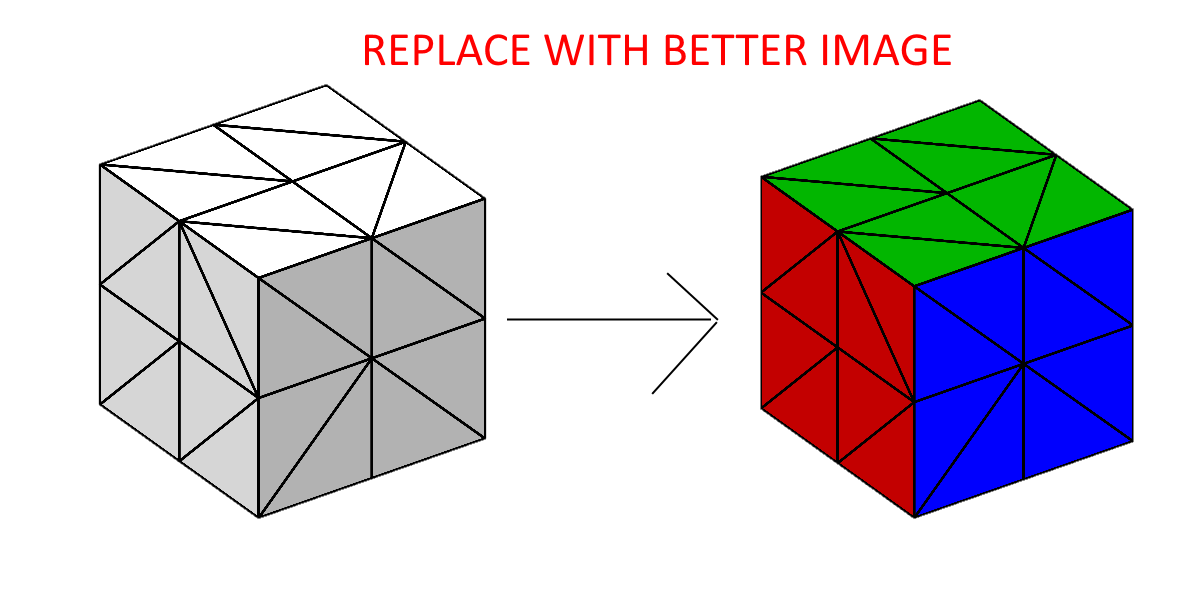
\includegraphics[width=1.0\columnwidth]{Images/plates_coplanar.png}
    \caption{Finding inherent surfaces.}
    \label{fig:coplanar}
\end{figure}

\subsection{Coplanar Faces}

The algorithm for finding coplanar faces requires the models to be stored as a face-vertex mesh. This is calculated by \meshlib, the library used for importing models. In a face-vertex mesh, faces only store their vertices' indices, with the vertices being stored in a different lookup table. This allows for easier adjacency checks - only the vertex indices have to be compared. Additionally, the face normals are stored in an array, in the same order as in the face list.

Now, two more lookup tables are added: One contains all edges (stored as a sorted pair of vertex indices) belonging to each face, while the second one allows looking up the faces adjacent to an edge. Both lists can be created in one single pass (see Listing \ref{lst:lookuptables}). 

\begin{listing}[ht]
\begin{minted}[
linenos
]{coffeescript}
setupFaceEdgeEdgeFaceLookup: ->
  for faceIndex in [0...faceCount]
    # Avoid double edges by sorting vertices
    { min_vertex
      mid_vertex
      max_vertex } = @findMinMidMaxVertex()
    # Register which edges this triangle uses.
    @addEntryToEdgeFaceMap(min_vertex, mid_vertex, faceIndex)
    @addEntryToEdgeFaceMap(mid_vertex, max_vertex, faceIndex)
    @addEntryToEdgeFaceMap(min_vertex, max_vertex, faceIndex)
    # Set the edges that make up this triangle.
    @faceVertexMesh.faceToEdges[faceIndex] = [
      [min_vertex, mid_vertex]
      [mid_vertex, max_vertex]
      [min_vertex, max_vertex]
    ]
\end{minted}
\caption{Simplified lookup table generation.}
\label{lst:lookuptables}
\end{listing}

Afterwards, the faces are grouped. This in done by iterating over all faces. When a face is found which has not been visited yet, a new face group is started. Now all of the face's edges are pushed to a queue, along with the current face index (Listing \ref{lst:iteratefaces}).

\begin{listing}[ht]
\begin{minted}[
linenos
]{coffeescript}
for faceIndex in [0...faceCount] when not faceVisited[faceIndex]
  faceGroup = [faceIndex]
  faceGroupIndex = faceGroups.length
  outerEdgeGroup = []
  groupNormal = @faceVertexMesh.getFaceNormal(faceIndex)
  @faceToFaceGroup[faceIndex] = faceGroupIndex
  faceVisited[faceIndex] = true
  # connect the adjacent faces
  edgeQueue = []
  adjacentEdges = @faceVertexMesh.getEdgesFromFace(faceIndex)
  for edge in adjacentEdges
    edgeQueue.push({ edge, faceIndex })
  @traverseAdjacentFaces(...)
\end{minted}
\caption{Iteration over faces with creation of new face groups.}
\label{lst:iteratefaces}
\end{listing}

There are multiple important variables being set here: First, we have the new \mintinline{coffeescript}{faceGroup}, containing only the current face. Next, we have the index of the group, used for creating a \mintinline{coffeescript}{faceToFaceGroup} lookup table. The \mintinline{coffeescript}{outerEdgeGroup} contains all edges surrounding the group, which allows the creation of a shape containing the face group. The group's normal vector is initialized with the current face's normal vector. Lastly, the current face is marked as visited in order to avoid checking it multiple times.

After the edges have been pushed in the queue, we start processing it (see Listing \ref{lst:traverseadjacent}).  

\begin{listing}[ht]
\begin{minted}[
linenos,breaklines
]{coffeescript}
traverseAdjacentFaces: tco (...) ->
  if edgeQueue.length is 0
    return
  { edge, faceIndex } = edgeQueue.shift()
    faceNormal = @faceVertexMesh.getFaceNormal(faceIndex)
  # get the faces from the edge
  adjacentFaces = @faceVertexMesh.getFacesFromEdge(
    edge[0]
    edge[1]
  )
  continued = false
  for nextFaceIndex in adjacentFaces when nextFaceIndex isnt faceIndex
    # check if faces are coplanar
    # [...]
  if not continued and edge[0] isnt edge[1]
    # the edge is an outer edge for this coplanar group
    outerEdgeGroup.push(edge)
  @recur(...)
\end{minted}
\caption{Function repeated for each edge in queue.}
\label{lst:traverseadjacent}
\end{listing}

\todo{list tco code? or just mention?}

This is implemented as a \emph{tail recursion}, the helper function \mintinline{coffeescript}{tco} is based on an existing implementation of tail calls in \coffeescript\footnote{TCO in \coffeescript, \url{https://gist.github.com/adrusi/1905351}}. It runs \mintinline{coffeescript}{traverseAdjacentFaces} as long as \mintinline{coffeescript}{recur} is called each pass. First, the length of the queue is checked. If there a no more edges waiting to be processed, we can jump out of the recursion and continue searching for new groups (Listing \ref{lst:iteratefaces}). Otherwise, we first get the normal of the face from which we came. Next, we extract the new face from the edge and get the face's normal as well. After checking the faces' coplanarity, we signal that there may be more elements in the queue by calling \mintinline{coffeescript}{recur}.

Listing \ref{lst:coplanarcheck} shows what happens when testing for coplanarity. \mintinline{coffeescript}{isAngleZero} calculates the angle between the normals and compares it to zero. This is done even if the new face was already visited. If the faces are not coplanar, the edge is added to the group's outer edges. In case of coplanarity, we now check if the face was visited. If it was not, it is added to the face group. Additionally, an entry is added to the \mintinline{coffeescript}{faceToFaceGroup} lookup table and the face is marked as visited. After fetching the face's edges, they are pushed into the queue.

\begin{listing}[ht]
\begin{minted}[
linenos,breaklines
]{coffeescript}
if @isAngleZero(faceNormal, nextFaceNormal)
  if not faceVisited[nextFaceIndex]
    faceGroup.push(nextFaceIndex)
    groupNormal.add(nextFaceNormal)
    @faceToFaceGroup[nextFaceIndex] = faceGroupIndex
    faceVisited[nextFaceIndex] = true
    adjacentEdges = @faceVertexMesh.getEdgesFromFace(nextFaceIndex)
    for nextEdge in adjacentEdges when not Util.arrayEquals edge, nextEdge
      edgeQueue.push({ edge: nextEdge, faceIndex: nextFaceIndex })
else
  outerEdgeGroup.push(edge)
\end{minted}
\caption{Check for coplanar faces.}
\label{lst:coplanarcheck}
\end{listing}

After all faces have been processed and assigned a group, the \mintinline{coffeescript}{faceGroups}, \mintinline{coffeescript}{faceGroupNormals} and \mintinline{coffeescript}{outerEdgeGroups} are injected into the face-vertex mesh, along with the \mintinline{coffeescript}{faceToFaceGroup} lookup table.

\subsection{Shape Finder / Deus}

DO STUFF HERE

\subsection{Hole Detection / Dimitri}

PASTE HERE

\section{Finding inherent plates}

In order to find inherent plates in a mesh, the first step is to find all coplanar shapes which are parallel and check if the distance between them fits one of the given plate thicknesses (Listing \ref{lst:platecand}).

\begin{listing}[ht]
\begin{minted}[
linenos,breaklines
]{coffeescript}
candidates = []
for shape1, index1 in shapes
  for shape2, index2 in shapes when index1 < index2
    if @normalsParallelAndSurfacesFacingApart shape1, shape2
      thickness = @checkPlateThickness shape1, shape2
        if thickness?
          candidates.push { shape1, shape2, thickness }
return candidates
\end{minted}
\caption{Finding plate candidates.}
\label{lst:platecand}
\end{listing}

\subsection{Checking parallelism}

While the testing for normal parallelism is done with built-in vector functions, the check if the shapes are facing apart uses a vertex of each of the surfaces and calculates the angle of the resulting vector to one of the normals. If this angle is smaller than 90\textdegree, the surfaces are indeed facing apart.

\subsection{Calculating best plate thickness}

The calculation of the optimal plate thickness is shown in Listing \ref{lst:checkplatethickness}. First, the actual distance between the shapes is calculated. Next, all possible plate thicknesses are tested if they can approximate the actual thickness well enough. Lastly, the thickness with the lowest absolute deviation is chosen as the best thickness.

\begin{listing}[ht]
\begin{minted}[
linenos,breaklines
]{coffeescript}
checkPlateThickness: (shape1, shape2) ->
  actualThickness = @distanceBetweenPlanes shape1, shape2
  okThicknesses = []
  # check which thicknesses are ok factor-wise
  for plateThickness in @plateThicknesses
    if plateThickness * @minThicknessDeviationFactor < actualThickness < plateThickness * @maxThicknessDeviationFactor
      okThicknesses.push plateThickness
  bestThickness = null
  bestDeviation = null
  for plateThickness in okThicknesses
    deviation = Math.abs(plateThickness - actualThickness)
    if bestDeviation is null or deviation < bestDeviation
      bestDeviation = deviation
      bestThickness = plateThickness
  return bestThickness
\end{minted}
\caption{Finding the best plate thickness.}
\label{lst:checkplatethickness}
\end{listing}

\subsection{Creating plates}

After finding these plate candidates, the shape which plane's distance to the origin (the z-value of all vertices when laid into the x-y-plane) is smaller is selected as the base shape of the plate, as shown in Listing \ref{lst:faceintersect}. Now, the intersection of both shapes is calculated. This is done by using the already calculated mapping of vertices into the x-y-plane. The resulting intersection is transformed back into 3D-space using the rotation matrix of the base shape. With the resulting shapes, plates are created.

\begin{listing}[ht]
\begin{minted}[
linenos
]{coffeescript}
shape2CloserToOrigin = abs(shape2.zValue) < abs(shape1.zValue)
polygon1 = create2DPolygon(shape1)
polygon2 = create2DPolygon(shape2)
intersection = polygon1.intersect polygon2
shapes = parseToShapes(intersection)
plates = parseToPlates(shapes)
return plates
\end{minted}
\caption{Face intersection for creating inherent plates.}
\label{lst:faceintersect}
\end{listing}

The intersection between the shapes is done using the \jsclipper library. After parsing them into the library's polygon class, they can be easily clipped, resulting in a list of intersections which can be parsed back into shapes. The plate creation is based on the previously selected base shape. While the calculated intersection is used as the shape of the plate, the thickness is computed by subtracting the base shape's z-value from the other shape's z-value. Additionally, the base shape's z-value is used as plane constant.

\section{Extruding plates}

The extrusion of plates is a simpler approach, which is shown in Listing \ref{lst:extrude}. The selected plate thickness has to be inverted, due to the plate being extruded against the face's normal direction. The plane constant of the plates base plane is the same as the z-value of the shapes x-y-representation. After checking the shape's area, the new plate is created.

\begin{listing}[ht]
\begin{minted}[
linenos
]{coffeescript}
createPlateFromShape: (shape) ->
  thickness = -@plateThicknesses[0]
  planeConstant = shape.edgeLoops[0].xyPlaneVertices[0].z
  if shape.getContour().computeArea() > @areaThreshold
    return new Plate shape, thickness, planeConstant
  else
    return null
\end{minted}
\caption{Extruding a plate from a shape.}
\label{lst:extrude}
\end{listing}

\section{Removing contained plates / Dimitri}

PASTE HERE

\section{Stacking plates}

As an alternative approach, plates can be stacked. This method does not directly use the models surfaces. However, they can be used for optimization.
The main function for stacking is shown in Listing \ref{lst:stackedmain}. First, the model is rotated in order to optimize the stacking direction. Afterwards, the clipping planes are calculated. After clipping the models faces with these planes, the resulting edges are merged into edge loops, which are used for creating shapes and, as wall as helper objects, polygons. With these, shafts can be added, which connect plates for easier assembly. Afterwards, plates are created. These have to be rotated back based on the original rotation in order to align them with the model. 

\begin{listing}[ht]
\begin{minted}[
linenos
]{coffeescript}
findStackedPlates: (model, shapes) ->
  return new Promise (resolve) =>
    rotationMatrix = @findRotation shapes
    model.getClone().then((clone) =>
      @model = @rotateModel clone, rotationMatrix
      @planes = @getClippingPlanes()
      @clipFacesAgainstPlanes @model.model.mesh.faces
      @mergeEdgesInPlanes()
      @shapeGroups = @createShapes()
      @polygonGroups = @createPolygons()
      @shafts = @findShafts()
      @shapes = @clipShafts()
      plates = @createPlates().filter((p) -> p?)
      shaftPlates = @createShaftPlates()
      plates = plates.concat shaftPlates
      plates = @rotatePlatesBack plates, rotationMatrix
      resolve plates
    )
\end{minted}
\caption{Plate stacking main function.}
\label{lst:stackedmain}
\end{listing}

\subsection{Rotating the model}

In order to find a good rotation, the model's biggest surface is aligned to the x-y-plane. While the approach of stacking plates doesn't require information about the model's coplanar surfaces, this optimization does. By iteration over them, the biggest surface's rotation matrix can be found (see Listing \ref{lst:findrotation}). This matrix can be used for transforming all vertices so that the chosen surface is parallel to the x-y-plane.

\begin{listing}[ht]
\begin{minted}[
linenos
]{coffeescript}
findRotation: (shapes) ->
  maxArea = 0
  rotationMatrix = new THREE.Matrix3()
  shapes.forEach((shape) ->
    area = shape.area || shape.getContour().computeArea()
    if area > maxArea
      maxArea = area
      rotationMatrix = shape.rotationMatrix
  )
  return rotationMatrix
\end{minted}
\caption{Finding an optimal rotation.}
\label{lst:findrotation}
\end{listing}

\subsection{Finding the clipping planes}

Due to the model being rotated, it can be sliced using planes parallel to the x-y-plane. In order to calculate these, the model's bounding box is calculated first. Using the minimal and maximal z-value, planes are creates with an distance equal to the selected plate thickness. These planes are constructed from a \threejs plane object and a (initially empty) list of edges located in this plane. The planes are displaced by half the plate thickness. Thus, the sampling happens in the middle of the plates-to-be, which is an approximation which works for most applications. The plane creation is shown in Listing \ref{lst:clippingplanes}.

\begin{listing}[ht]
\begin{minted}[
linenos,breaklines
]{coffeescript}
getClippingPlanes: ->
  planes = []
  for i in [@minZ..@maxZ] by @thickness
    planes.push {
      plane: new THREE.Plane(
        new THREE.Vector3(0, 0, 1), 
        -(i + @thickness / 2)
      )
      edges: []
    }
  return planes
\end{minted}
\caption{Clipping plane generation.}
\label{lst:clippingplanes}
\end{listing}

\subsection{Clipping the model's faces}

Clipping each face with each plane would be very slow. Thus, we first find one plane which clips the face and check the adjacent planes afterwards (see Listing \ref{lst:clipfaceplanes}). I order to quickly find this plane, binary search is used, as shown in Listing \ref{lst:findplane}. Starting at the median plane (\mintinline{coffeescript}{@planes.length // 2}), we search the planes until one plane clipping the face is found or it is certain that no plane clips the face.

\begin{listing}[ht]
\begin{minted}[
linenos
]{coffeescript}
clipFaceAgainstPlanes: (face) ->
  planeIndex = @findClippingPlane(face)
  if planeIndex > -1
    @checkAdjacentPlanes(face, planeIndex)
\end{minted}
\caption{Clipping a face against all planes.}
\label{lst:clipfaceplanes}
\end{listing}

\begin{listing}[ht]
\begin{minted}[
linenos,breaklines
]{coffeescript}
findClippingPlane: (face) ->
  stepWidth = @planes.length / 4.0
  index = -1
  currentIndex = @planes.length // 2
  oldIndex = -1
  while currentIndex isnt oldIndex and 0 <= currentIndex < @planes.length and index is -1
    direction = @clipFaceAgainstPlane(
      face, 
      @planes[currentIndex]
    )
    # found clipping plane
    if direction is 0
      index = currentIndex
    # continue search
    else
      oldIndex = currentIndex
      currentIndex += Math.round stepWidth * direction
      stepWidth /= 2
  return index
\end{minted}
\caption{Finding a plane which clips the face.}
\label{lst:findplane}
\end{listing}

The search direction is calculated by clipping the face against the plane (Listing \ref{lst:clipfaceplane}). After clipping each edge with the face, the number of intersection decides the result.

\begin{itemize}
  \item No intersections: The face does not clip the plane.
  \item One Intersection: Invalid. It is not possible to get only one intersection when clipping a valid face.
  \item Two intersections: If both intersection points are the same, one vertex of the face clips the plane. Otherwise two edges clip the plane.
  \item Three intersections: If any two of the intersection points are the same, a vertex and the opposite edge clip the plane. Otherwise the whole face lies in the plane.
\end{itemize}

If the face doesn't clip the plane or only intersect with one vertex, we check if it is below or above the plane and return either -1 or 1 as direction (calculation shown in Listing \ref{lst:facedirection}). In all other cases, 0 is returned, because the face clips the plane and we don't have to search further. 

Additionally, if either two edges, an edge and a vertex or the whole face clips the plane, these intersections are stored in the plane.

\begin{listing}[ht]
\begin{minted}[
linenos
]{coffeescript}
clipFaceAgainstPlane: (face, plane) ->
  intersections = []
  face.vertices.forEach((vertex, index) =>
    start = vector(vertex)
    end = vector(face.vertices[(index + 1) % 3])
    line = new THREE.Line3(start, end)
    intersection = plane.plane.intersectLine line
    if intersection? then intersections.push intersection
  )
  # handle intersections
  # [...]
  return direction
\end{minted}
\caption{Clipping a face against a plane.}
\label{lst:clipfaceplane}
\end{listing}

\begin{listing}[ht]
\begin{minted}[
linenos
]{coffeescript}
getDirectionFromPlaneToFace: (face, plane) ->
  sum = 0
  face.vertices.forEach((vertex) ->
    sum += vertex.z + plane.plane.constant
  )
  if sum is 0 then throw new Exception()
  return sum / Math.abs sum
\end{minted}
\caption{Calculating the direction from a plane to a face.}
\label{lst:facedirection}
\end{listing}

After one clipping plane has been found, the adjacent ones have to be checked as well, since a face can span over multiple planes. This is done by iterating over the planes, starting from the next one and moving away. If the returned direction is not 0, we can stop because the plane and all following ones do not clip the face. Both directions, upwards and downwards, are checked seperately (see Listing \ref{lst:checkadjacent}).

\begin{listing}[ht]
\begin{minted}[
linenos,breaklines
]{coffeescript}
checkAdjacentPlanes: (face, index) ->
  runIndex = index + 1
  direction = 0
  while(runIndex < @planes.length and direction is 0)
    direction = @clipFaceAgainstPlane(
      face, 
      @planes[runIndex++]
    )
  runIndex = index - 1
  direction = 0
  while(runIndex >= 0 and direction is 0)
    direction = @clipFaceAgainstPlane(
      face, 
      @planes[runIndex--]
    )
  return
\end{minted}
\caption{Checking if adjacent planes are clipping too.}
\label{lst:checkadjacent}
\end{listing}

\subsection{Creating shapes}

Using the intersections stored in each plane, shapes can be created. These shapes represent the cross-sections of the model. Since this requires merging the intersection edges, the shapes finder can be re-used for this step. Additionally, the \jsclipper library is used to create 2D polygons, which are used in the next step.

\subsection{Adding shafts}

In order to assemble the stacked plates, we connect them with shafts (Figure \ref{fig:shafts}). Our approach for this: if two shapes which are located in adjacent planes intersect, they have to be connected by at least one shaft. The shaft finding algorithm has three steps: First, we iterate over all shapes and connect as many as possible. Next, we fix shapes which are not yet connected. Afterwards, we clean up shafts which are only connected to one shape.

\begin{figure}
    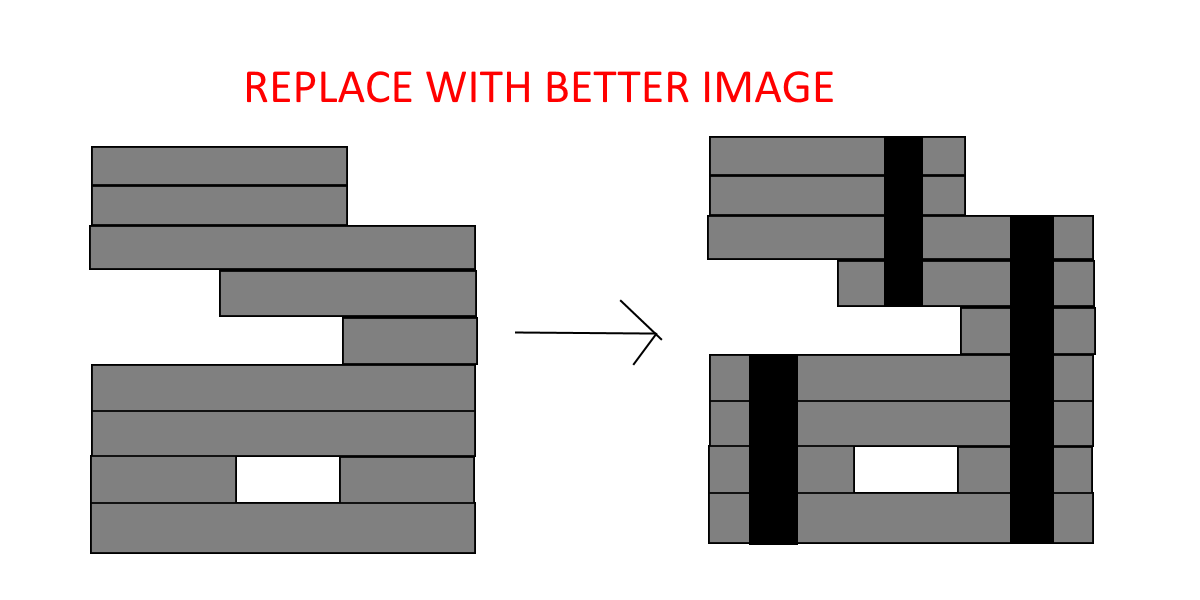
\includegraphics[width=1.0\columnwidth]{Images/plates_shafts.png}
    \caption{Connecting plates with shafts.}
    \label{fig:shafts}
\end{figure}

\subsubsection{The shaft object}

A shaft has these properties:
\begin{itemize}
    \item polygons - a list of the polygons which the shaft connects
    \item intersection - the intersection of all the polygon which the shaft connects
    \item finished - true if the shaft is complete and won't be extended to connect more polygons
    \item lastlevel - the layer of the last added polygon
    \item shaftData - contains the shaft's cross section's x and y dimensions
\end{itemize}
It contains functions which allow adding new polygons to the shaft, and building the shaft's cross section and contour.

\subsubsection{First pass}

Instead of the actual shapes, the corresponding polygons are used, which enable working with the \jsclipper. These are organized in layers, matching the clipping planes. Each layer contains a list of polygons, since there can be multiple shapes in one layer. We have to iterate over both lists, the inner and the outer, as shown in Listing \ref{lst:findshafts}.

When processing a new polygon, we first mark that it has not been added to any shaft yet. Now, we iterate over all shaft candidates. If the current level (the layer) is bigger than the shaft's last added polygon's level plus one, there was no polygon from the last layer added to the shaft. Since we do not want shafts to create "bridges" spanning between unconnected layers, the shaft is marked as completed. If that is not he case, we try to add the polygon to the shaft.

\begin{listing}[ht]
\begin{minted}[
linenos,breaklines
]{coffeescript}
findShafts: ->
  shaftCandidates = []
  @polygonGroups.forEach((polygonGroup, level) =>
    polygonGroup.forEach((polygon) =>
      added = false
      shaftCandidates.forEach((shaftCandidate) =>
        if level > shaftCandidate.lastlevel + 1
          shaftCandidate.finished = true
        if not shaftCandidate.finished
          if @tryAddingPolygonToShaftCandidate(
                polygon, shaftCandidate
              )
            shaftCandidate.lastlevel = level
            added = true
      )
      if not added
        if Shaft.isIntersectionBigEnoughForShaft(
              polygon.polygon, @shaftData
            )
          newShaftCandidate = Shaft.fromPolygon(
            polygon,
            level,
            @shaftData
          )
          newShaftCandidate.polygons[0].shafts.push(
            newShaftCandidate
          )
          @tryOverlappingShaftBackwards newShaftCandidate
          shaftCandidates.push newShaftCandidate
    )
  )
  @fixUnconnectedPlates shaftCandidates
  @cleanUpShafts shaftCandidates
  shaftCandidates.forEach((shaft) ->
    shaft.createShaftContourAndCrossSection()
  )
  return shaftCandidates
\end{minted}
\caption{Finding shafts.}
\label{lst:findshafts}
\end{listing}

Listing \ref{lst:addpolytoshaft} shows the calculations run when adding a polygon to a shaft. First, the shaft's intersection and the new polygon are intersected. The resulting intersection is checked if it is big enough to fit the shaft. If that is the case, the shaft's intersection is updated and the polygon is added to the shaft.

\begin{listing}[ht]
\begin{minted}[
linenos,breaklines
]{coffeescript}
tryAddingPolygonToShaftCandidate: (
    polygon, shaftCandidate, direction
  ) ->
    clip = polygon.polygon.intersect shaftCandidate.intersection
    if clip.length > 0 and
        Shaft.isIntersectionBigEnoughForShaft clip[0], @shaftData
      newIntersection =
        new jsclipper.Polygon clip[0].getShape(), clip[0].getHoles()
      shaftCandidate.intersection = newIntersection
      if direction is "DOWN" then shaftCandidate.polygons.unshift polygon
      else shaftCandidate.polygons.push polygon
      polygon.shafts.push shaftCandidate
      return true
    return false # no intersection
\end{minted}
\caption{Adding a polygon to a shaft.}
\label{lst:addpolytoshaft}
\end{listing}

If the polygon can not be added to any of the shafts, we create a new one - if the polygon is big enough (Listing \ref{lst:findshafts}). Additionally, the shaft is overlapped "backwards", up to three layers. This improves stability in the assembled model.

\subsubsection{Fixing unconnected plates}

In some cases, not all polygons - and thus not all plates - are connected to the others yet. Additionally, shafts should be expanded in both directions as far as possible. A fix is shown in Listing \ref{lst:fixunconnected}.

Each polygon is checked how well it is connected to other polygons. If it is connected to both a polygon below and above (\mintinline{coffeescript}{connection.isConnected} is true), we do not have to connect it further. Otherwise, the shafts connecting it from above and below are checked. We try to expand these to connect more polygons in the given direction. If this succeeds, handling for this polygon is completed. Otherwise, we create a new shaft at this polygon and try to expand it in both directions.

\begin{listing}[ht]
\begin{minted}[
linenos,breaklines
]{coffeescript}
fixUnconnectedPlates: (shaftCandidates) ->
  @polygonGroups.forEach((polygonGroup, level) =>
    polygonGroup.forEach((polygon) =>
      connection = @isPolygonConnected polygon, level
      if not connection.isConnected
        expanded = false
        direction = "DOWN"
        if connection.shaftsFromAbove.length > 0
        expanded = @tryExpandingShaftsInOneDirection(
          connection.shaftsFromAbove, level, direction
        )
        if connection.shaftsFromBelow.length > 0
          direction = "UP"
          expanded = @tryExpandingShaftsInOneDirection(
            connection.shaftsFromBelow, level, direction
          )
        if not expanded and 
            Shaft.isIntersectionBigEnoughForShaft(
              polygon.polygon, @shaftData
            )
          newShaftCandidate = Shaft.fromPolygon(
            polygon
            level
            @shaftData
          )
          newShaftCandidate.polygons[0].shafts.push(
            newShaftCandidate
          )
          @tryExpandingShaftAroundLevel(
            newShaftCandidate
            level
            direction
          )
          shaftCandidates.push newShaftCandidate
    )
  )
\end{minted}
\caption{Fixing unconnected plates.}
\label{lst:fixunconnected}
\end{listing}

\subsubsection{Cleaning up shafts}

As a result of this method, polygons which are not adjacent to any other polygon get assigned an own shaft. Since this does not improve the models stability, these are removed again, as shown in Listing \ref{lst:cleanupshafts}.

\begin{listing}[ht]
\begin{minted}[
linenos
]{coffeescript}
cleanUpShafts: (shafts) ->
  if shafts.length > 0
    for i in [shafts.length - 1..0]
      if shafts[i].polygons.length < 1
        log.error "FOUND SHAFT WITH ZERO POLYGONS"
      if shafts[i].polygons.length < 2
        shafts[i].polygons.forEach((polygon) ->
          polygon.shafts.splice polygon.shafts.indexOf(shafts[i]), 1
        )
        shafts.splice i, 1
\end{minted}
\caption{Cleaning up shafts.}
\label{lst:cleanupshafts}
\end{listing}

\subsection{Creating plates}

After the shafts are found, their cross section is cut from the connected polygons. Next, these polygons are parsed into shapes and plates. Additionally, the shafts' contours are calculated, with additional plates being created from them. Together, all plates are returned.

\end{document}
\cleardoublepage

%\part{Graph}
\subfile{Chapters/06.1-Graph}
%\documentclass[../ClassicThesis.tex]{subfiles}
\begin{document}
%************************************************
\chapter{Adjacency Plategraph / Klara}\label{ch:graph}
\newcommand{\TODO}[1]{\textcolor{red}{\\ \textbf{TODO:} #1 \\}}
%************************************************


% Use active Voice (we do….)
% Ein Gedanke pro Paragraph
% Terminologie anpassen über alle Arbeiten hinweg (was ist eine Plate für alle…)
% Jeder sollte eine kleine Related Work section haben
% Erklärungen zu warum dieser Algorithmus genutzt wurde und nicht ein anderer + limitations des gewählten Algorithmus
% Hübsche Bildchen zum anschaulichen Erklären!! (ebenfalls konsistent halten: gleich geformte labels etc.)
% FROM SOLUTION TO PROBLEM /DISCUSSION
% EXPLAIN ALL VARIABLES ETC.!!!

% 1. Was macht es inhaltlich
% 2. Was kann/tut der Graph überhaupt?


% \paragraph{Why is this part necessary?}
On the basis of the plategraph we can create connectors for plates in the later step \hyperref[ch:joints]{joint creation}. Depending on angles and neighborhood relationships an adequate connector type can be chosen.
% for what? to figure out joint connections?

% \paragraph{What is being achieved in this Chapter?}
In this step we analyse the spatial arrangement of plate objects in 3D-space to create a graph structure which tracks the adjacency. The plates to be analysed are found in the previous step \hyperref[ch:plates]{Plates}. Two or more plates are adjacent to another when at least one side touches or overlaps with the other plate. In addition, the angles in between the plates are calculated. 


% WHAT IS WITH THE 3D SNIPPETS??? DO THEY STILL EXIST?

% \paragraph{Chosen Graph Class Structure} 
The graph holds a list of all found plates and their neighbors. \\
For graph iteration we traverse all edges of the graph which also hold the neighborhood parameters such as angle and the line at which nodes intersect.\\\* \\
\hspace*{-1.8cm}
\begin{figure}[!ht]
\centering
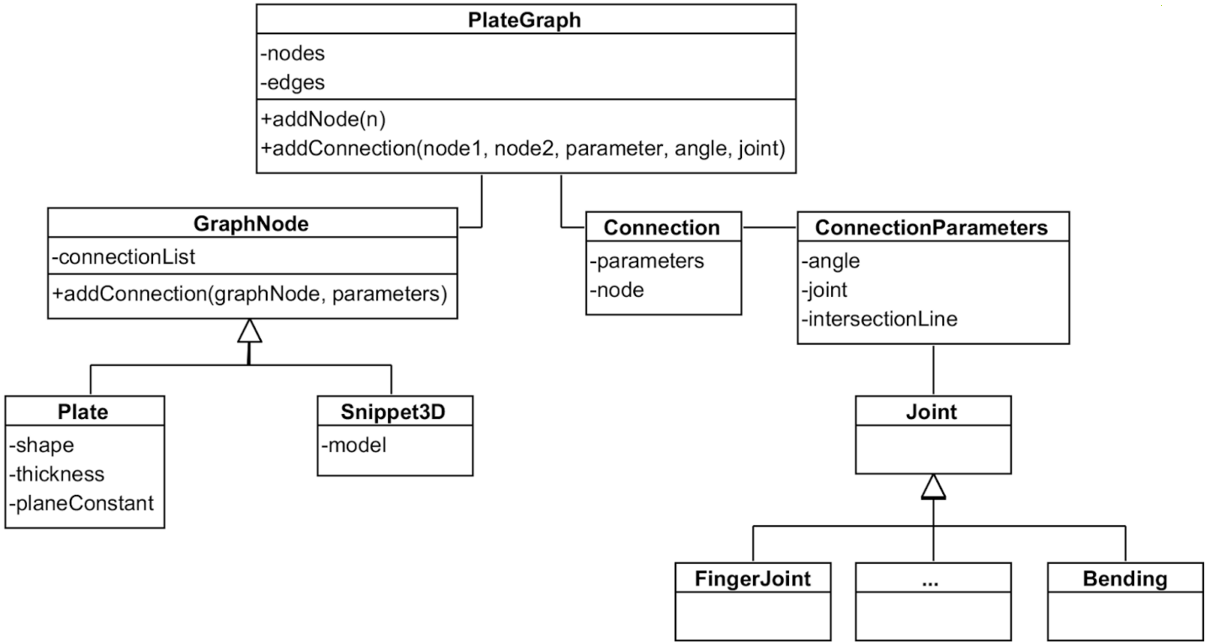
\includegraphics[width=1\columnwidth]{Images/GraphStructure.png}
\caption{Class diagram of the plategraph structure. Nodes and Connections can be added to the graph when a new intersection has been found. }
\end{figure}

\TODO{Plategraph beinhaltet nodes, edges ... und was machen der graph, was sind nodes und edges, dadurch kann auf diese weisen... das ... erreicht werden...}

\section{Detecting spatial arrangement}
% \subparagraph{requirements for running the algorithm}
% unnecessary??
As a prerequisite the step \hyperref[ch:plates]{Plates} needs to find inherent or create extruded plates first. Afterwards the plane-plane intersections of all combinations of both sides of the plates are computed which results in up to four intersection lines. In preparation for the joint generation step \ref{ch:joints} we truncate the inner intersection lines which would otherwise overlap with adjacent plate intersections.

\subsection{Finding intersections}\label{findIntersections}
% \subparagraph{concrete explanation, functions used/example code etc.}
When two planes intersect there is an intersection line. Since we work with plates which equal two parallel planes we expect to find up to four intersection lines.\\
First, we retrieve the direction vector \emph{dir} of an intersection line between two plates by calculating the cross vector of both normals.
\TODO{include citation}
In order to retrieve all possible intersection lines of two plates we then calculate four possible plane-plane intersections \cite{planePlaneIntersection} of 
\begin{itemize}
\item the two main sides of the plates
\item the two parallel sides of the plates
\item one main and one parallel side 
\item one parallel side and one main side
\end{itemize}
\*\\
First, a possible position vector \emph{p} has to be found which lies on both planes.
\\\*\\
\emph{Plane constants:} $d_1, d_2$\\
\emph{Normals:} $\vec{n_1}, \vec{n_2}$
$$ p = \frac{d_1 * \vec{n_{2}}^{2} - d_2 * (\vec{n_1} * \vec{n_2})}{\vec{n_{1}}^{2} * \vec{n_{2}}^{2} - (\vec{n_1} * \vec{n_2})^{2}} * \vec{n_1} + \frac{d_2*\vec{n_1}^2 - d_1*(\vec{n_1} * \vec{n_2})}{\vec{n_1}^2 * \vec{n_2}^2 - (\vec{n_1} * \vec{n_2})^2} * \vec{n_2} $$
\TODO{cite this}

On the basis of a position vector \emph{p} and the direction $\vec{dir}$ an intersection line can be computed: $ line = p*x + \vec{dir}$
\\
Now that all lines are found we have to test if the lines actually go through both plates and that the plates touch. \\
\TODO{Why should it not go through both plates?}
In addition, this step retrieves the exact start and end points of the line segment that defines the intersection of both plates.\\
\TODO{When and how?}
In order to find the boundaries of the lines we calculate the intersections of the lines with all boundary edges of the plates.\\
\begin{figure}[!ht]
\centering
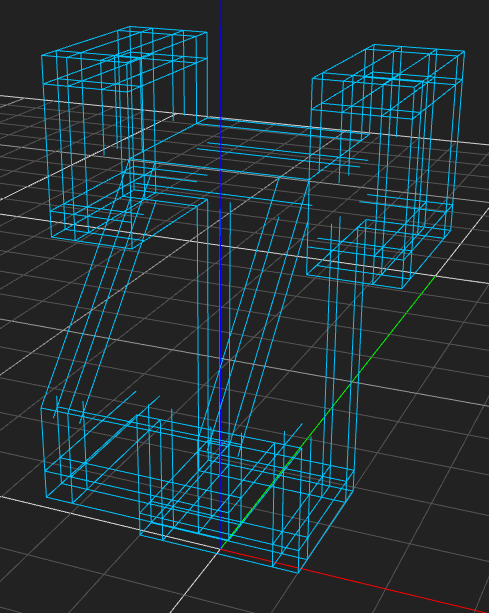
\includegraphics[width=.5\columnwidth]{Images/HeadAllBoundaries.png}
\caption{All intersections that were found. }
\end{figure}

\begin{figure}[!ht]
\centering
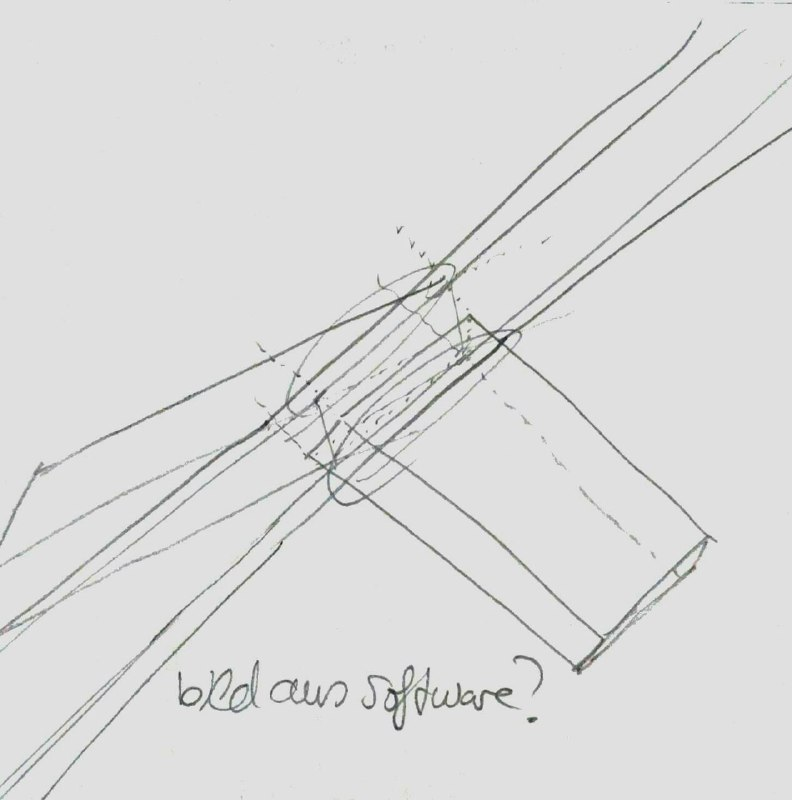
\includegraphics[width=.5\columnwidth]{Images/06-1-graph-fourIntersectionLines.jpg}
\caption{Single plate pair with all of its intersection lines. The marked part is the segment that we continue to work with.}
\end{figure}


\section{Preparing plates for connectors}
\subsection{Volume based clipping}
Before joints can be added to the plates we have to prepare them. We cut the shapes back so that the joints do not overlap with the other plate.\\
As seen before, up to four intersectionlines have been calculated per intersection. Two of them lie both on one side of the plate and the other two belong to the second side. The two lines on one side build a rectangle when their ends are connected. We use those two rectangles to remove the parts of the plates where we will place fingerjoints.
\begin{figure}[!ht]
\centering
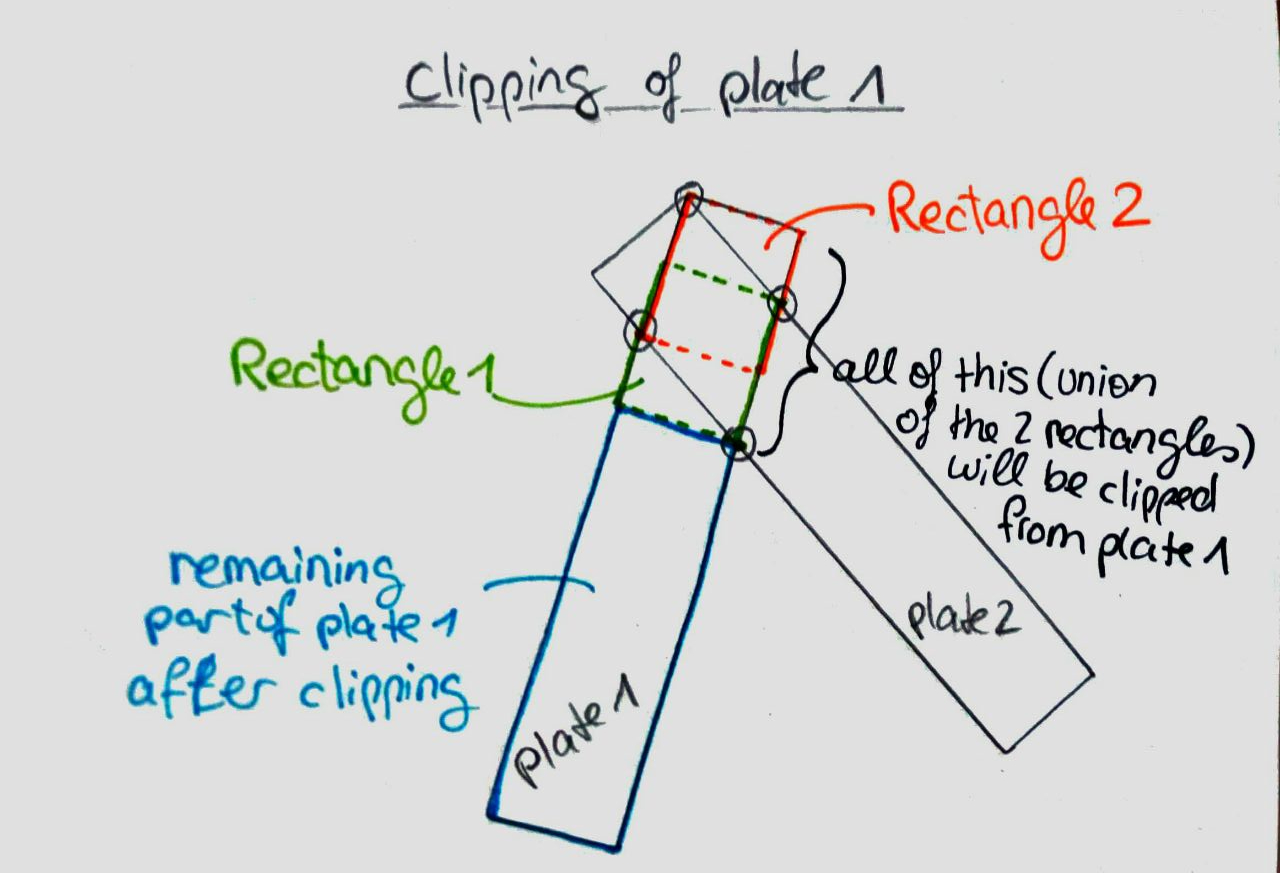
\includegraphics[width=\columnwidth]{Images/10-joints-clippingPlate.jpg}
\caption{Side view of a single plate pair. The circles mark where there are intersection lines. The rectangles show what is clipped away from plate 1. }
\end{figure}

There are cases when not all four lines are actually a plate intersection but only a plane intersection. 
\begin{figure}[!ht]
\centering
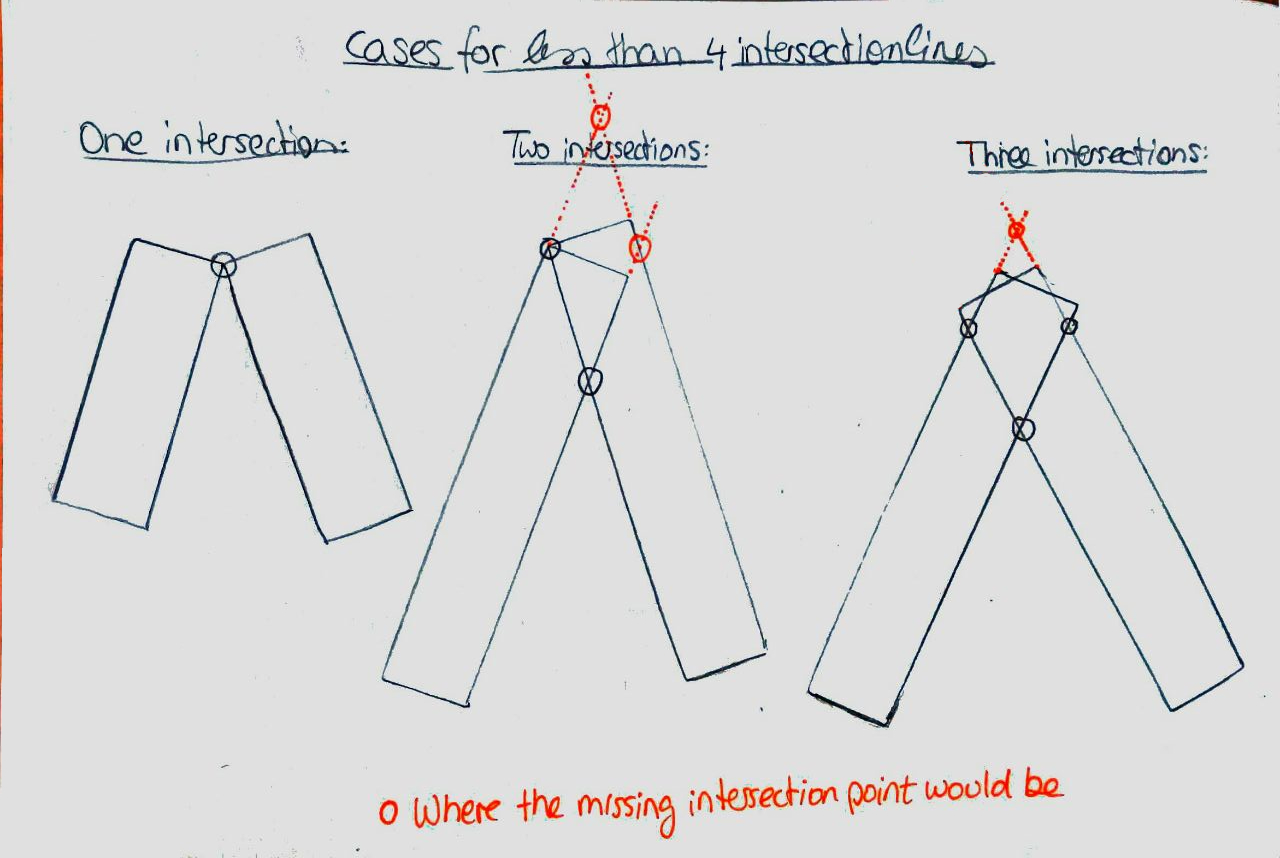
\includegraphics[width=\columnwidth]{Images/10-joints-casesOfLines.jpg}
\caption{There can also be less than 4 actual intersections. In this case we have to calculate the projected intersectionlines as well which are only a correct plane-plane-intersection but not actually where the plates overlap}
\end{figure}

In this case the infinitifly long plane intersection line will be clipped to match the length of the existing plate intersections. This yields two rectangles as well, which can then be used for clipping the shapes of the plates.
\begin{figure}[!ht]
\centering
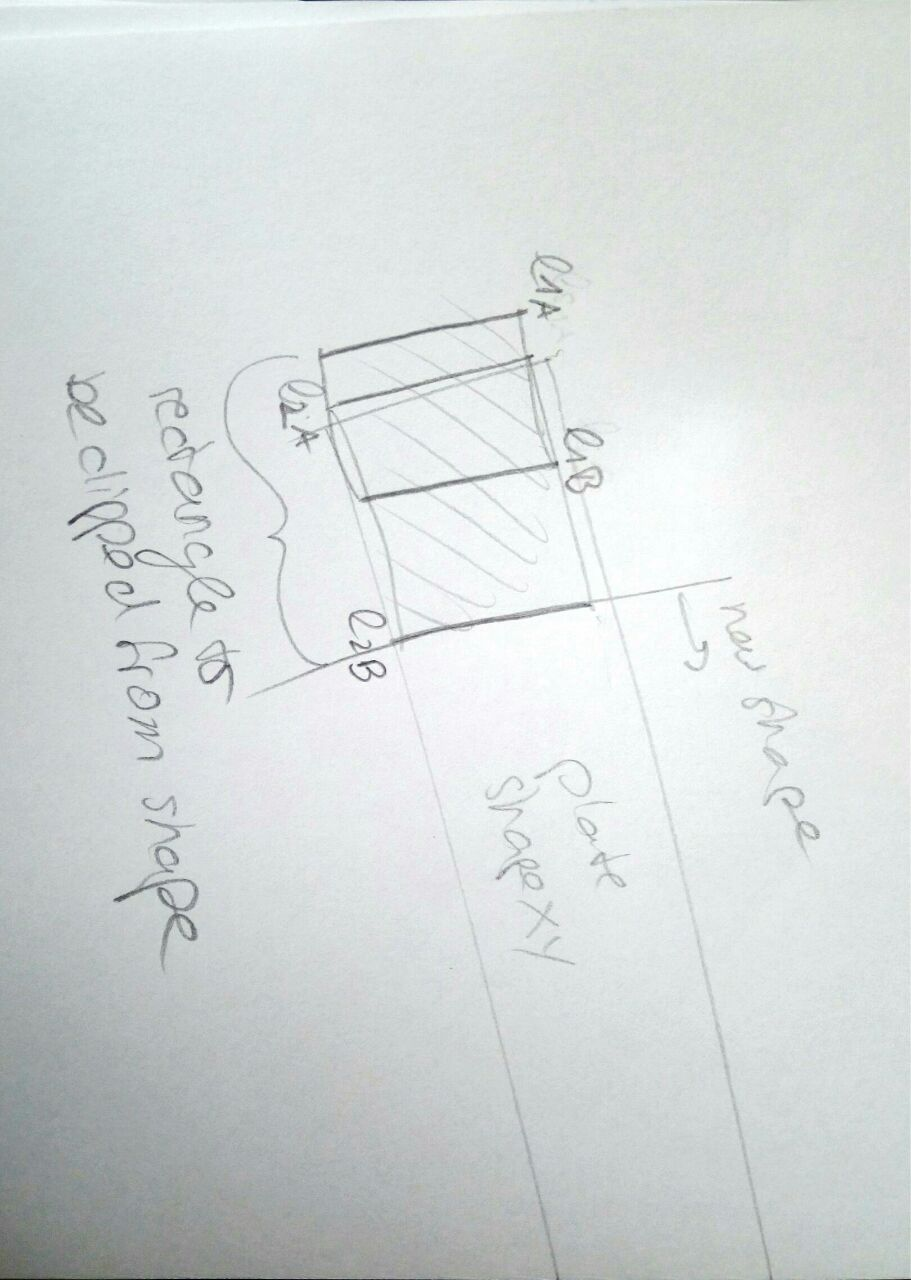
\includegraphics[width=.5\columnwidth, angle=90]{Images/06-1-graph-clippingRectangles.jpg}
\caption{The shape of the plate is rotated so it lies on the xy-plane. The rectangles derived from the intersection line segments define what has to be clipped away from the shape.}
\end{figure}

\begin{figure}[!ht]
\centering
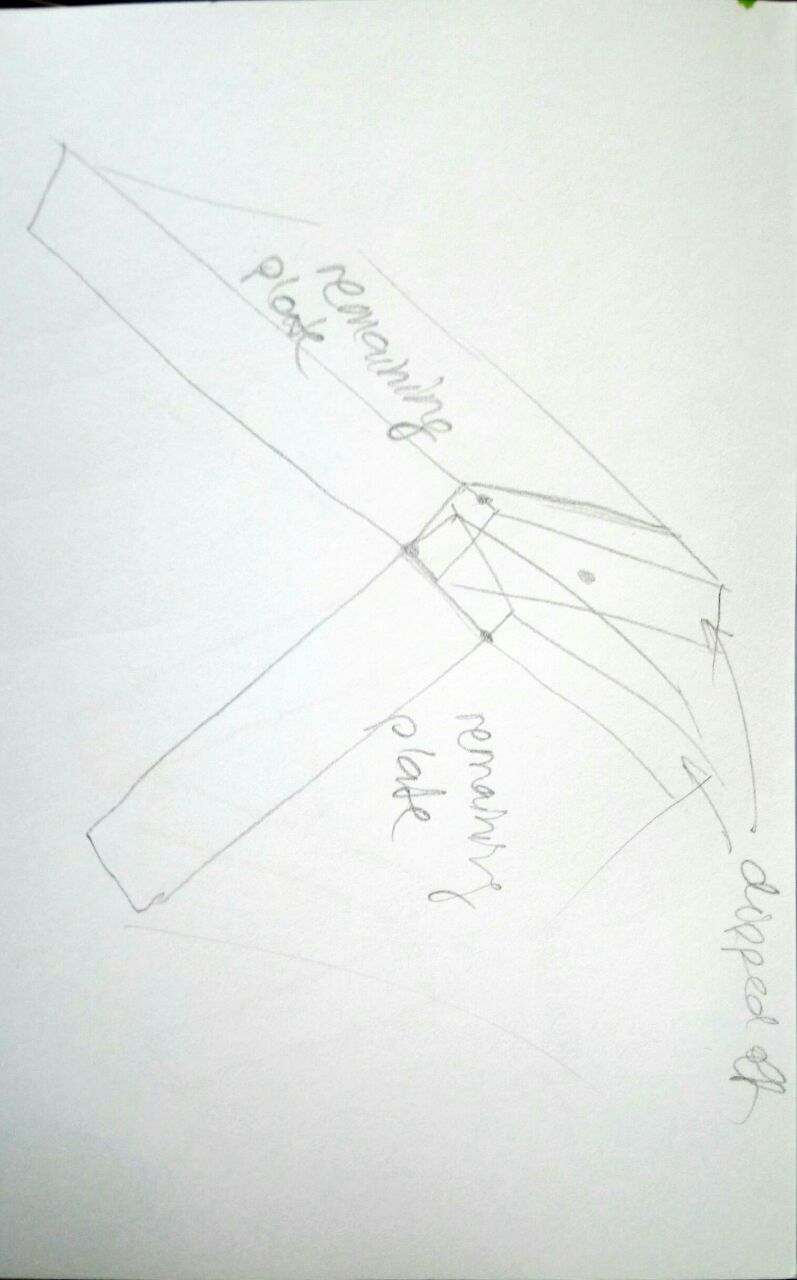
\includegraphics[width=.5\columnwidth, angle = 90]{Images/06-1-graph-clippingResult.jpg}
\caption{When the shapes have been cut in 2D they are rotated back to form a 3-dimensional plate again. This figure depicts the volume which was cut off by the algorithm leaving the remaining plates p$_1$ and p$_2$}
\end{figure}


\section{Analyzing spatial arrangement}
\subsection{Angle calculation}\label{angleCalculation}
In order to generate fitting joints in the upcoming step and for grouping plates to curves (see Chapter \hyperref[ch:curves]{Curves}) the angles are necessary.\\
First, we determine the angle between the according planes.\\
plane normals: $\vec{u}, \vec{v}$\\
angle between planes: $\theta$
$$ cos(\theta) = \frac{\vec{u} \cdot \vec{v}}{|\vec{u}| * |\vec{v}|}$$
But we are not talking about infinitely large planes instead we want the angle which is enclosed by the finitely large plates. Therefore we need to adjust the angle in some cases.\\
\TODO{rewrite previous 2 sentences!!}
Thanks to the previous clipping step we can find out when the angle has to be adjusted.\\
We observed that plates with an acute angle still touch when cut back and that plates with an obtuse angle do not touch after cutting them back.
\begin{figure}[!ht]
\centering
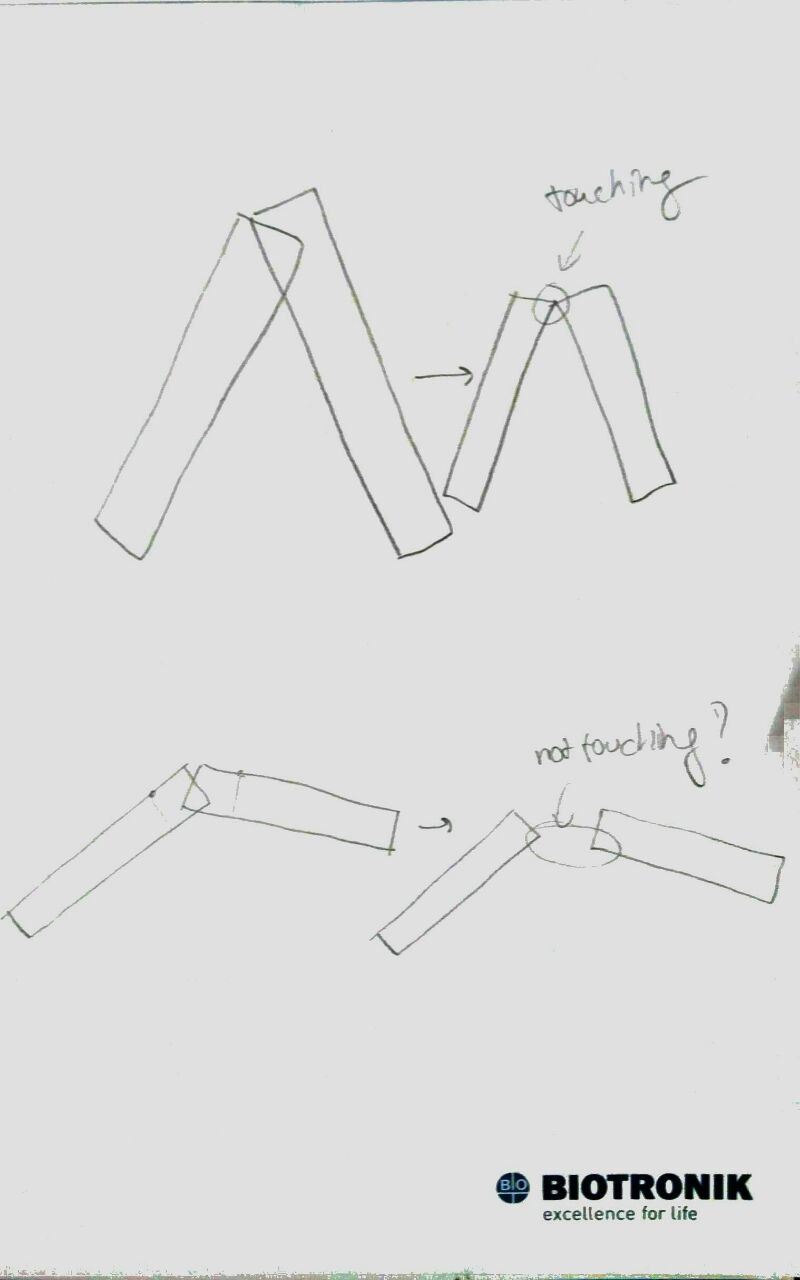
\includegraphics[width=.5\columnwidth]{Images/06-1-graph-TouchingOrNotAfterClipping.jpg}
\caption{After the clipping process the plate pair might be not touching anymore. This means that the angle between the plates has to be larger than 90$^\circ$.}
\end{figure}

Finally, we test if the plates still touch and adjust the angle accordingly.

\subsection{Finding new main lines}\label{mainLine}
In order to know where to add the joints to the plate we have to identify one line segment for each plate whithin a connection.\\
For that we compare the distances of the new edges of the two plates. Where the distance is the smallest they are the two lines which determine where to place the joints.
\begin{figure}[!ht]
\centering
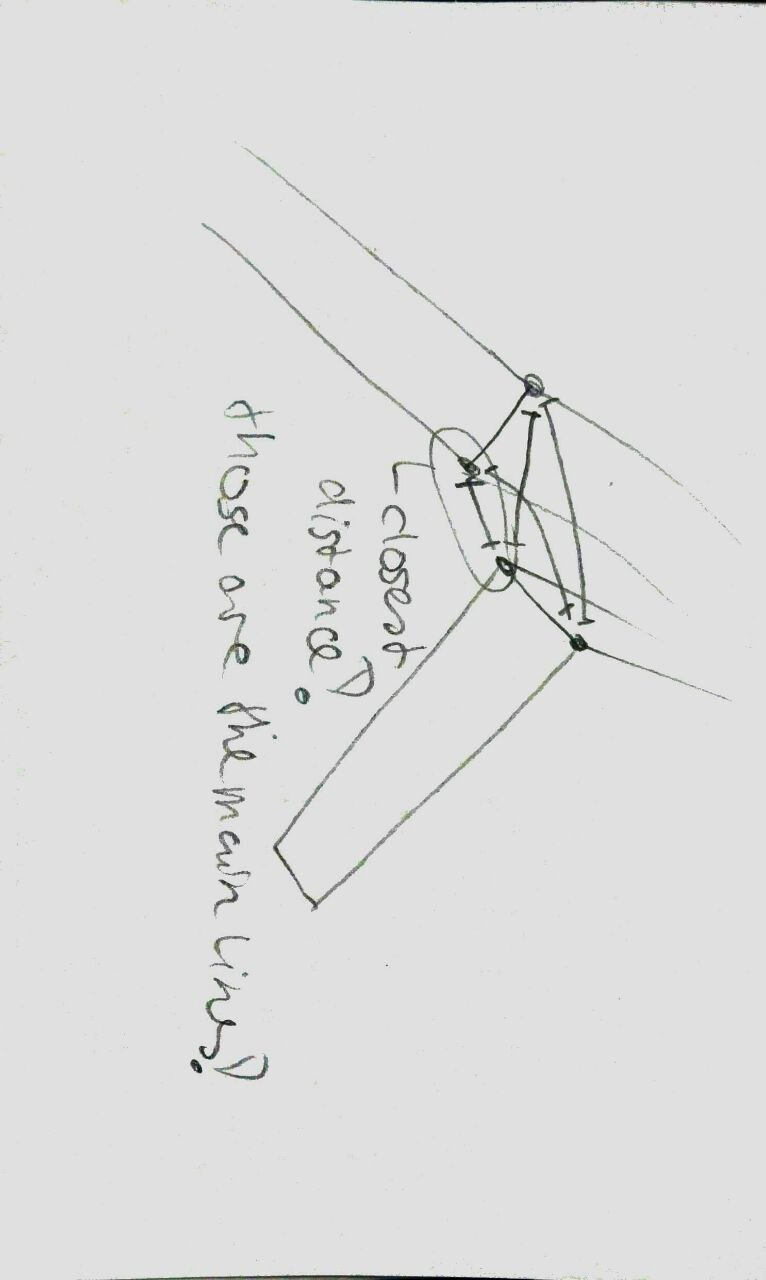
\includegraphics[width=.5\columnwidth, angle=90]{Images/06-1-graph-mainLinesAfterClipping.jpg}
\caption{The distances between the new edges after the clipping process reveals which of them are the inner lines. Those lines will be used for adding joints in the next step.}
\end{figure}

The segments are called main line for that connection and plate.

\subsection{Truncating intersection lines}
Now that all main lines are known we need to shorten the lines so that no other lines overlap with it. If this step is missing then the following step for creating joints will run in to problems because the joints overlap each other.\\
If we now have a look at only the inner intersections of plates in a model we can identify the overlaps.
\begin{figure}[!ht]
\centering
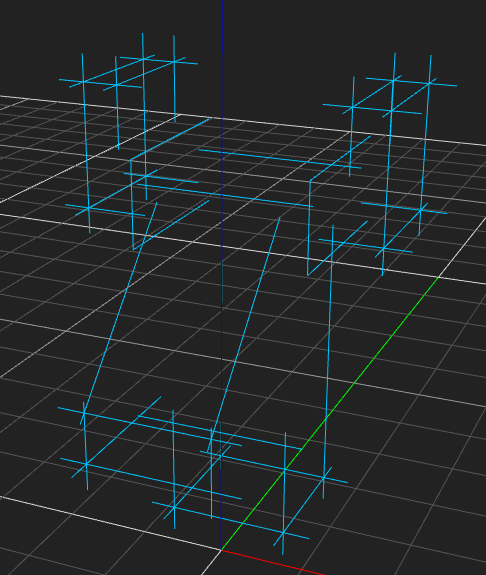
\includegraphics[width=.5\columnwidth]{Images/HeadInnerBoundaries.png}
\caption{The inner boundaries of the plates overlap. In the next step when joints will be created they are only supposed to be on the inner part of the line. Therefore the lines have to be truncated.}
\end{figure}
\*\\
\begin{algorithm}[H]
	\DontPrintSemicolon
	\KwData{lines}
	\KwResult{truncated lines}
	initialize variables here\;
    \For{line$\_$pair in lines}{
    	line1 = line$\_$pair[0]\;
        line2 = line$\_$pair[1]\;
        point = lineLineIntersection(line1, line2)\;
        \If{isPointOnLine(point, line1) and isPointOnLine(point, line2)}
        {
       		\tcp{linesegments actually cross}
       		startSegmentLine1 = new Line(point, line1.start)\;
            endSegmentLine1 = new Line(point, line1.end)\;
            startSegmentLine2 = new Line(point, line2.start)\;
            endSegmentLine2 = new Line(point, line2.end)\;
            \tcp{the shorter part of each line is discarded}
			\eIf{startSegmentLine1.distance() $>$ endSegmentLine1.distance()}{
				\eIf{startSegmentLine2.distance() $>$ endSegmentLine2.distance()}{
				return \{
                    	endSegmentLine1\;
                        endSegmentLine2
                    \}
				}{
                    return \{
                    	endSegmentLine1\;
                        startSegmentLine2
                    \}
				}
			}{
			return \{
                	startSegmentLine1\;
                    startSegmentLine2
                \}
			}	      
        }
    }
   	\caption{Truncating lines}
\end{algorithm}

Finally, we found all plate adjacencies and necessary information on the connected parts. Also, we adjusted the plates. Therefore the next step explained in Chapter \hyperref[ch:joints]{Joint Creation} can start adding joints.

\section{Alternative approaches}
The solutions presented in this chapter may not be the only way to go. Therefore, we want to give an overview of other algorithms we tried or are aware of and why we replaced them.

\subsection{Possible data structures for intersection tracking}
\TODO{cite Beyer}
Dustin Beyer used an adjacency matrix for keeping track of neighboring plates. All the plates were kept in a plate array. Their indices corresponded to the rows and columns of the matrix. Each cell contained a set of plate adjacency objects. This made it possible that one plate could have more than one connection.\\
\*\\
Instead of an adjacency matrix we used the previously explained plategraph class structure because it allows for traversal along the plates and, additionally, the found edges. \\
Moreover, our structure is open for adding additional objects beside plates. For example 3D-printable snippets which were not converted to plates by our software.

\subsection{Approaches for finding intersections}
\TODO{cite}
In the master thesis on Platener a connection is calculated by finding all four possible connections between both sides of two plates. Then the edges of the plates are tested against the line. The part of the line overlapping with an edge was kept for further calculations.\\
\*\\
When looking for plate intersections we also calculate all possible intersections. But plates do not always touch each others edges. Therefore we replaced this algorithm by a different approach explained in the previous section for \hyperref[findIntersections]{finding intersections}.

% \subsection{Bruteforce finding lines}
% The first approach was gathering all lines from all plate boundaries and looking for intersects of any other line. This is a very costly calculation but less prone to rounding errors. \\
% Later we continued on to using plane intersections which meant we only needed to work with all combinations of plates instead of all of its edges.

\subsection{Representation of the joint location}
As seen before in the section \hyperref[mainLine]{Main Lines} we calculate one line per intersection and plate which determines where we will place the joints. We chose this approach because it is a straight forward way. The joints only have to be moved onto the line and can directly be added to the plates. \\
A different, more future oriented, approach is to work with the axis going through the middle of where the joints will be. This means it also defines the axis around which the plates could rotate when their angle changes. 
\TODO{Include image that shoes hinge twice. One where the axis is marked and one where our two main lines are marked!}
In the case that our software will be extended with an editor the user might want to select an edge and define that the connection should be similar to a hinge. For this you would want rather one axis than two lines specific to a plate. But then the calculation for where to place the joints at the plate becomes more expensive.\\
In our use case the single line approach for an edge of a plate is completely sufficient.

\subsection{Finding main lines by checking if they lie on a corner of the shape}
As already mentioned when plates intersect there can be up to four intersection lines. We need to define which of them is the most important one in order to know where to put joints. The line we wanted to choose had to touch both plates.
\TODO{Image of the four lines and showing which one should always be the main line}
This means all lines which intersected with any points of the shapes of the plates were ignored. The other line became main line.\\
Our assumption which we adopted from the Platener thesis \TODO{cite}  for finding the main line is the following:\\
Two plates always touch one another edge-to-edge. Therefore, if an intersection line does not lie on an outer boundary of the shape it is the main line.
\begin{figure}[!ht]
\centering
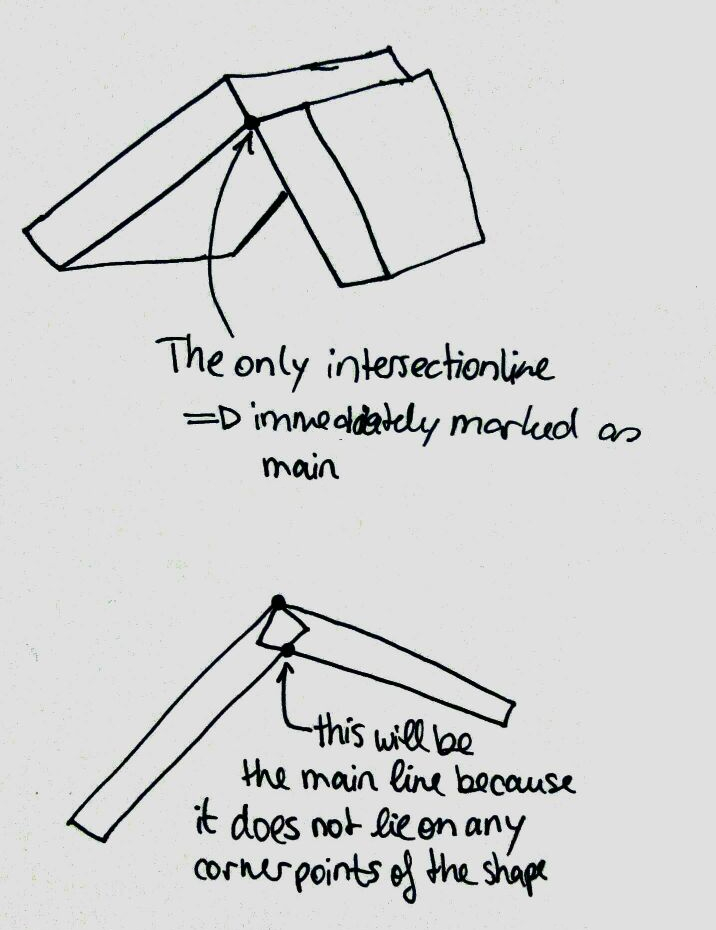
\includegraphics[width=.5\columnwidth]{Images/06-1-graph-assumptionMainLine.jpg}
\caption{Our assumption was that we only need to define one main line per plate pair. If there was just one intersection at all it was obvious. And when there were more than one intersection we thought the inner intersection should be the main line. }
\end{figure}

But the problem is that plates can intersect in many different ways which do not all verify our first assumption. 
\begin{figure}[!ht]
\centering
\includegraphics[width=.5\columnwidth]{Images/06-1-graph-assumptionMainLine.jpg}
\caption{In this case the angle between the plates is obtuse. If we just took the inner intersection here without first clipping of the plates there would be no space for joints. }
\end{figure}
\TODO{replace this with image of two planes where this doesnt work}
This is why we replaced this algorithm with the one from the previous section \hyperref[mainLine]{Main Lines}.

\subsection{Adjusting angles based on which sides of the plates touch}
Our previous version of finding a main line was supposed to yield one line. Based on this line the angle was calculated with the following procedure:\\ 
After the angle of the planes had been calculated we adjusted the angle in some cases dependent on the direction in which the normals were pointing. \\
We know which sides of the plates are enclosing the angle thanks to the previous main line calculation.
% figure which shows when angle is right, but also one case when it is not right
\begin{figure}[!ht]
\centering
\includegraphics[width= 1\columnwidth]{Images/anglesExamplesSmall.png}
\caption{(a) The angle between the plates' normals correspond with the angle $\gamma$ between the plates. (b) The angle between the plates' normals is in this case an adjacent angle to the requested angle $\gamma$.}
\end{figure}

In order to find out in which cases the angle has to be adjusted we check for two properties.\\
First, there is the question which of the sides of the plates intersect. A plate is defined by a 2D-shape which is called main side. The other side which exists due to a specified thickness of the plate is called parallel side.\\
Additionally, we look at the direction of the normals. The direction is positive when it is directed from the main to the parallel side and negative otherwise.\\
For an angle to be in need to be adjusted the following conditions need to be satisfied.
\begin{itemize}
    \item The two plates touch with the same type of side 
    \item[] AND
    \item Their directions are both positive OR both negative
\end{itemize}
But as mentioned before all of these calculations are based on the assumption that the previous main line calculation only yielded one line.\\
\TODO{Include image that shows when this is not the case, with captions explaining why our current algorithm fails here}
In this case the previous algorithm fails which is why we developed a new approach for finding the correct angle as already explained in the section \hyperref[angleCalculation]{Angle Calculation}.

\section{Future work}

\begin{itemize}
    \item To be not forgotten: A line can be split into pieces!:\\
    Plates do not only touch another along one line. 
    \begin{figure}[!ht]
    \centering
    \includegraphics[width=0.5\columnwidth]{Images/06-2-joints-moreThanOneLinePerEdge.jpg}
    \caption{Plate 2 touches Plate 1 twice. This should result in two edges and intersections which should be handled seperately.}
    \end{figure}
    
    \item find out if model is assemblable in the end\\
    A very important information about the final converted model is if it can actually be build. A user may not only need assembly instructions on how to actually build the model when cut but also if it is possible to do so. There may be a conflict when plate a needs to be put up before plate b but plate b also needs to be in the model before plate a. This should not happen or at least be mentioned to the user.
    \item rejoining broken up plates (t-connection)\\
    This is what Dustin also suggested and already implemented.\\
    He suggested to group two plates together again when:\\
    \begin{enumerate}
        \item the main sides of P1 and P2 are coplanar
        \item P1 and p2 have the same thickness
        \item P1 and P2 each have a shared edge with p3 that is parallel and which overlaps when projected onto each other
    \end{enumerate}
    It can happen that during finding inherent plates some plates are broken by another. This should result in a t-junction. For this the plategraph has to recognize those broken-up plates and reunion them. \\
    For this the following steps are necessary:
    \begin{enumerate}
        \item Iterate over all nodes and check if it has two or more neighbors. 
        \item Test if any of the neighbors are coplanar to each other. If so they are labeled as plates p1 and p2. Any other neighbor is labeled p3 or higher.
        \item Check if p1 and p2 have the same thickness. If not start over with the next node
        \item If they have the same thickness the intersections needs to be checked for parallelness and overlaps between p1 and p3 and p2 and p3.
        \item When determined that p1 and p2 are actually one plate which is parted by p3 then they need to be unioned and marked for a t-junction to be handled in the next step.
    \end{enumerate}
    (not sure if this is all it takes maybe a plate is broken up more than once, meaning not only p1 and p2 might be coplanar)
\end{itemize}





% Dummy algorithm:\\
% \begin{algorithm}[H]
% 	\DontPrintSemicolon
% 	\KwData{input Data}
% 	\KwResult{result Data}
% 	initialize variables here\;
%    \caption{Name of Algorithm}

% \end{algorithm}



% \begin{algorithm}[H]
% \DontPrintSemicolon
% 	\KwData{this text}
% 	\KwResult{how to write algorithm with \LaTeX2e }
% 	initialization\;
% 	\While{not at end of this document}{
% 	read current\;
% 	\eIf{understand}{
% 	go to next section\;
% 	current section becomes this one\;
% 	}{
% 	go back to the beginning of current section\;
% 	}
%      \For{all I know}{
%      look at this link to learn more about \LaTeX2e:\;
%      http://ctan.space-pro.be/tex-archive/macros/latex/contrib/algorithm2e/doc/algorithm2e.pdf\;
%      }
% 	}
%    \caption{How to write algorithms}

% \end{algorithm}






\end{document}
\cleardoublepage

%\part{Joints}
\subfile{Chapters/06.2-Joints}
%\documentclass[../ClassicThesis.tex]{subfiles}
\begin{document}

%************************************************
\chapter{Joint Computation / Klara}\label{ch:joints}
\newcommand{\TODO}[1]{\textcolor{red}{\\ \textbf{TODO:} #1 \\}}
%************************************************

% Use active Voice (we do….)
% Ein Gedanke pro Paragraph
% Terminologie anpassen über alle Arbeiten hinweg (was ist eine Plate für alle…)
% Jeder sollte eine kleine Related Work section haben
% Erklärungen zu warum dieser Algorithmus genutzt wurde und nicht ein anderer + limitations des gewählten Algorithmus
% Hübsche Bildchen zum anschaulichen Erklären!! (ebenfalls konsistent halten: gleich geformte labels etc.)

\section{Joint computation}
\TODO{buy green and orange (or at least two different colors) of acrylic for demo objects and pictures in the paper}
A lasercutted object needs connectors if it consists of multiple parts. Those can be elements like screws, nails and glue. Or the plates already come along with connectors. Those can be for example fingerjoints which, when well calibrated, do not need any external material to hold together. \\
Whenever possible we want to provide connections like that because a user needs less effort when components work directly out of the lasercutter. This is why we provide three types of joints which are added to the determined plates.
\TODO{im Gesamtsystem einordnen, was war davor, was kommt danach?}

\section{building joints}
\TODO{Make this section easier to read!}
The general procedure of creating joints consists of three steps: First we calculate how many female and male joints fit onto the intersection. Then the retrieved joints are placed at the intersection line and the shapes are merged to result in the original plate with joints.
\subsubsection*{Building the joints for a specific intersection line}
% \paragraph{jointCount}
% We need to know how many joints we have to place onto the intersection. We call this 'jointCount' which describes the number of all joints which fit on the line including the male and female joints. 
First we find out how many joints, males and females, fit along the length of the line.
Since all joint types have equal widths for female and male joints we divide the length of the line by the width of a joint.\\
\*\\
% \paragraph{adjustJointWidth}
But the result from this calculation has to be rounded because the number of joints just found do not necessarily work out evenly with the length of the line. This yields us a whole number which defines how many joints we need to create. Then we adjust the width so that the joints will be evenly spread without leaving space on either end of the line.\\
Now that we know how the joints will look like and how many we need it is time to find out how to distribute them.\\
In order to always create a well defined female and male part we place a thick joint in the center of the line if there are an even number of joints to be distributed.\\
%\textbf{TODO: provide image of the two cases: even and odd number}
\begin{figure}[!ht]
\centering
\includegraphics[width=\columnwidth]{Images/10-joints-evenOddJointCount.jpg}
\caption{Distribution of joints depending on the number of joints. An even number results in a thick inner joint.}
\end{figure}

% \paragraph{computeMaleJointsPerSide} %number only
On both sides of the middle joint will be an equal number of male joints. How many depends on the jointCount. An even jointCount means 2 joints less and odd means one joint less on the sides because the middle joint will be created seperately. Since the jointCount specifies the number of all joints, male and female we have to divide by two to get the number of male joints only and then divide by two once more to achieve the seperation into the two sides.\\
maleJointsPerSide = 
\begin{cases} 
(jointCount - 2) / 4, & jointCount $ \% 2 == 0 $ \\ 
(jointCount - 1) / 4, & jointCount $ \% 2 == 1 $
\end{cases}\\
\*\\
% \paragraph{buildJointsForEven / Odd count}
Finally, we can start placing the middle joint and distributing as many joints as just calculated on either side of it evenly with leaving enough space inbetween the joints for a female one to fit in.
\begin{figure}[!ht]
\centering
\includegraphics[width=\columnwidth]{Images/10-joints-spreadedJoints.jpg}
\caption{The joints are spreaded evenly along the line leaving space of a joint with in between for the other plates joints to fit in.}
\end{figure}
% \paragraph{computeFemaleJointsPerSide} %number only
The computation for the number of female joints on one side of the middle joint is very similar to the previous computation for male joints. Only that the middle joints do not have to be subtracted.\\
femaleJointsPerSide = 
\begin{cases} 
(jointCount) / 4, & jointCount $ \% 2 == 0 $ \\ 
(jointCount + 1) / 4, & jointCount $ \% 2 == 1 $
\end{cases}\\
\*\\
% \paragraph{create Females for fingerjoint type}
When creating \emph{fingerjoints} the female joints are the exact negative of the male joints. Therefore we do not create these joints one by one. Instead we retrieve the boundingbox of the male joints along the length of the intersection line and calculate the difference of this rectangle and the male joints. The result are the female joints.\\
\*\\
% \paragraph{create Females for jimjoints/dovetail joints}
In the case of \emph{dovetail}- and \emph{jim-joints} we have to create the female joints by placing each single joint along the intersection line.\\
This is achieved by distributing them in the same way as the male joints are evenly spread. Except that for the females we leave the space for the middle joint empty.\\
Finally, we have created female and male joints which are aligned along a line with the length of the intersection.
    
\subsubsection*{Placing the joints at the correct edge of the plate}
This step moves the joints to the correct position in space. 
% \paragraph{line and shape into XY}\\
\*\\
To do shape union functions we need to move the shape of the plate and the intersectionline into the xy-plane.
\*\\
% \paragraph{bounding box of joints, center of bounding box}
The joints which already lie in the xy-plane are rotated and translated onto the intersectionline.\\
\*\\
% \paragraph{make sure joints are placed at line but outside of shape}
To make sure that the joints will be appended to the plates we test if the transformed joints lie inside the plate. If so they are moved towards the outside of the plate.
            
\subsubsection*{Merging the joints with the plate}
The last step unions the now aligned shapes of the joints and plates and rotates them to the correct position in space where the plate belongs to within the model.


\section{Different Fingerjoint types}

\TODO{Bilder noch so anpassen, dass nur females/males zu sehen und in echt, wie sie zusammen stecken}\\
We support three types of joints. Each have benefits when used for specific material. For example acylic is not flexible which means it is very sturdy, but bendable when heated. \\
We allow the user to choose the type of material which then affects the choice of joints in the converted model.

\subsubsection{Fingerjoint template}
\begin{minipage}{0.4\textwidth}
\begin{figure}[!ht]
\centering
\includegraphics[width=1\columnwidth]{Images/fingerjoints.png}
\caption{Path which a lasercutter has to follow to cut our plates with fingerjoints.}
\end{figure}


\end{minipage}
\begin{minipage}{0.6\textwidth}
%\paragraph{How these joints look like}
Fingerjoints only consist of 90 degrees angles. The female joints are the exact inverse of the male joints. This means that the joints can slide directly into each other. 
\end{minipage}
But that only works when the sizes are measured correctly so that they create a tight fit. Otherwise plates connected by fingerjoints do not fit into each other at all or fall apart and have to be glued. 
%\paragraph{How these joints work, and for what material}
When using fingerjoints one typically has 90 degree angled plates because it is the easiest way to connect them. Other angles can be created but it is hard to know when the plates form the exact angle that is wanted unless the plates are part of a construction which gives them no other choice than to form the given angle.
\TODO{Maybe show this in a picture? Boat vs only two plates, where the angle cannot be determined without the other plates}
Regarding the material fingerjoints are useless when flexible materials are connected with it. The problem is that a tight fit cannot be created in most cases. Also very thin material is not working well since fingerjoints hold up due to the friction of one plate to the other. The fewer material the less friction.\\
We usually use fingerjoints for acrylic and wood.


\subsubsection{JimJoint template}
\begin{minipage}{0.6\textwidth}

These joints are named after Jim McCann who thankfully showed us the design for these connections.
%\paragraph{How these joints look like}
The male and female joints are the same but they grow wider with its height.
\end{minipage}
\begin{minipage}{0.4\textwidth}
\begin{figure}[!ht]
\centering
\includegraphics[width=1\columnwidth]{Images/jimjoints.png}
\caption{Path which a lasercutter has to follow to cut our plates with JimJoints.}
\end{figure}

\end{minipage}
This means these joints cannot slide into each other but they rather snap together. This means once they are connected they cannot be taken apart just by pulling on the plates. 

%\paragraph{How these joints work, and for what material}
In order for the snapping to work the material has to be flexible or very thin. Jim McCann already used it for foam. We now use it especially for paper because this material would be too thin for creating enough friction for fingerjoints to work.

\subsubsection{Dovetail template}
\TODO{Image of wood dovetails where this joint is derived from.}\\
    \begin{minipage}{0.4\textwidth}
    \begin{figure}[!ht]
    \centering
    \includegraphics[width=1\columnwidth]{Images/schwalbe.png}
    \caption{Path which a lasercutter has to follow to cut our plates with JimJoints.}
    \end{figure}
    
    \end{minipage}
    \begin{minipage}{0.6\textwidth}
    Typically a dovetail joint is used in woodwork. It helps to ensure that when there is a pulling force on both wooden plates that the joints all hold onto the other plate.\\
    \end{minipage}
    But in order to create the female joints the wood needs to be cut in an angle. This is not possible without inadequately high time and power consumption. See the upcoming section \hyperref[alternativeSolution]{Alternative Solution} for information on how to lasercut the female part of a dovetail.\\
    Instead, we developed a joint type very similar to the original dovetail. This can be easily cut with a lasercutter.
    %\paragraph{How these joints look like}
    The males and females are alot like typical fingerjoints. But the females have an additional part which will fixate the other plate from one direction.
    \TODO{insert image}
    %\paragraph{How these joints work, and for what material}
    These joints now withstand a force pulling away the plate with the female joints. It works with any material with at least around one millimeter of thickness when the material is not very flexible.

\subsection{adjusting fingerjoints length when plates are angled}
    % \paragraph{adjustJointHeight}
    Not only the width has to be adjusted but also the height needs to be adapted to the plates connection. Depending on the angle of the plates the joints need to be longer or shorter accordingly.\\
    This problem can be solved by using trigonometry within the geometry of the overlap of the plates.\\
    If the plates overlap they create a parallelogram. The length of the long diagonal \emph{d} is the key to finding the appropriate length for the joints.
    \begin{figure}[!ht]
    \centering
    \includegraphics[width=0.5\columnwidth]{Images/06-2-joints-newJointHeight1.jpg}
    \caption{The parallelogram spanned by the overlap of the plates allows us to find the appropriate height for a joint.}
    \end{figure}
    
    We have already calculated the angle between the plates earlier and can now use it to find the lengths of the sides \emph{a} and \emph{b} of the parallelogram by the help of trigonometry:\\
    Thickness of plate $p_1$: $t_1$\\
    Thickness of plate $p_2$: $t_2$
    $$ a = t_1 / sin(180^{\circ} - \alpha)$$
    $$ b = t_2 / sin(180^{\circ} - \alpha)$$
    \begin{figure}[!ht]
    \centering
    \includegraphics[width=0.5\columnwidth]{Images/06-2-joints-newJointHeight2.jpg}
    \caption{The diagonal d can be calculated by the sides of the parallelogram.}
    \end{figure}
    
    This helps us to calculate the length of the diagonal \emph{d}:
    $$ d = \sqrt{a^2 + b^2 - 2ab * cos(\alpha)}$$
    Finally, the triangle which helps us retrieve the height for the fingerjoints \emph{h} can be constructed. 
    \begin{figure}[!ht]
    \centering
    \includegraphics[width=0.5\columnwidth]{Images/06-2-joints-newJointHeight3.jpg}
    \caption{The diagonal d is the hypotenuse of the right triangle with the wanted height for the joints.}
    \end{figure}
    
    $$ h = \sqrt{d^2 - a^2} $$
    
    \TODO{Abschließender Satz?}
    

\section{Alternative solutions / related work}\label{alternativeSolution}
\subsection{more joint type}
\subsubsection{snap fits}
Snap fits we already tried. Hard to implement because enough space needs to be given when cutting the spring.
\TODO{show image of our cube with snap fits!}
\subsubsection{pettis joints}
other joint type: pettis joint (fingerjoint with screws)
\subsubsection{t-joint}
slot joinery technique when overlapping plates had to be rejoined
\subsubsection{real dovetails with the lasecutter}
In order to achieve different depths of cutting you can set the lasercutter to use lower power. This is usually used for engraving which is a method to not cut through the material.
\begin{figure}[!ht]
    \centering
    \includegraphics[width=0.5\columnwidth]{Images/06-2-joints-schwalbeMitLaser.png}
    \caption{Instructions on how to build dovetails with the lasercutter.}
    \end{figure}
\\
\TODO{Name Lasercut like a boss here}\\
By coloring a part in the svg-file in a gradient from white to black this part will be cut in an angle. The more white the less power.

\subsection{Wrong fingerjoint height adjustment}
Firstly, the angle can be projected onto values between $0^\circ$ and $90^\circ$. Then the cosine function returns a number between 0 and 1 for the angle. The thickness of the plate is divided by this number to achieve a height that fits the angle and the thickness of the plates. 

\subsection{Dustins useless angle stuff}
He computed different angle types. They are quite crappy because he assumed that plates would only meet at edges. But plates can lie in another\\
\TODO{Make images to figures and add caption}
\includegraphics[width=0.5\columnwidth]{Images/06-2-joints-angleTypesDustin.jpg}\\
\includegraphics[width=0.5\columnwidth]{Images/06-2-joints-angleTypesWrongAssumption.jpg}\\
Therefore we do not use those angle type but we clip both plates with their four intersection lines. \\
Then due to angle and trigonometry etc. we can calculate the correct length for the joints which connects the plates again.

    
    
    
\section{Future work}
    \begin{itemize}
        \item Dustin also suggested T-joints
        \item joints should not stand out on the side. \\
        Either their width has to be adjusted to be not only the width of when the joint starts building away from the plate. but also include how far away it is growing to the sides in its full height. \\
    (Beware that the joints still have to be placed according to its inner with otherwise they are too lose (except for fingerjoints) )
        \item when creating fingerjoints do not calc femaleJointsPerSide (unneccessary since using the stencilBox)
    \end{itemize}


\end{document}
\cleardoublepage

%\part{Curves}
\subfile{Chapters/07-Curves}
%\documentclass[../ClassicThesis.tex]{subfiles}
\begin{document}

%************************************************
\chapter{Curves/Deus}\label{ch:curves}
%************************************************

\section{Cutting curved shapes}

Approximating curved shapes with parts created by the laser cutter is a special challenge because only 2D shapes can be cut. There are several approaches to make the cut material bendable, for example, paper can be bent because of the material properties. Acrylic becomes bendable when heated, while bending wood is made possible by the use of a special cutting pattern, the so-called living hinges (see Section \ref{sec:living_hinges}).

Theoretically, this only enables the possibility to create shapes from developable surfaces, like cylinders, but no doubly curved ones, like spheres. But since our meshes consists of triangles, which are themselves two-dimensional, our meshes are always developable.

\section{General approach}

In our implementation, we use the  \emph{bend} joint type as an alternative to, for example, finger joints. Like the finger joint generation, the calculation of bends is based on the plate graph. The bent plate generation is separated into two steps. First, our implementation analyses which parts can be bent. Second, it creates a flat shape from the curved parts, which can be cut with a laser cutter. 

\section{Prerequisites creating bent plates}

%Because we use bends as a connection type the bent plate creation is based on the plate graph.
The algorithm uses the plates and connections from the plate graph. The plates provide their shape, normal and rotation matrix, which is used for laying it into the xy-plane. Additionally, the connections intersection line and angle are used. Before calculating bends, the finger joints have to be created, with the resulting shapes being stored in the corresponding connection.

\section{Living hinges}
\label{sec:living_hinges}

Living hinges are segments of a rigid material that are made flexible locally. There are several techniques to do this, e.g. thinning the material in this area. Using the \lasercutter{} a living hinge can be created by dense parallel cuts. They are disconnected every few centimeters and the breaks are offset to the next parallel cut (see Figure \ref{fig:living_hinge}).

\note{TO DO: add image of living hinge}

\section{Developable surface}

Formally developable surfaces are defined as surfaces with zero Gaussian curvature. Practically this means they can be created from a flat surface by cutting, bending and folding and without compressing or stretching. Examples for objects with and without developable surfaces are shown in Figure \ref{fig:developable_surface_examples}.

\note{TO DO: add images of developable and not developable surfaces}

\section{The bent plate object}

\class{Bent plate} is a data structure we use to represent a set of plates which are connected directly or indirectly with bend connections. Thus a bent plate can be cut as one piece. A \class{bent plate} consists of a set of \class{plates}. It provides the method \mintinline{coffeescript}{generateShape} which develops the surface of the connected shapes (see Section \ref{sec:generateShape}). Another method implemented by \class{bent plate} is \mintinline{coffeescript}{generateBendLines} which creates cuttable marks where two plates are merged (see Section \ref{sec:generateBendLines}).

\subsection{The generateShape function}
\label{sec:generateShape}

To generate the \class{shape} of the \class{bent plate} we first check how many \class{plates} this \class{bent plate} contains. If none are contained, the generated \class{shape} is \emph{null}. If there is just one \class{plate} then its \class{shape} is used.

If there are multiple plates in the bent plate the generation is done the following way: For each of the plates in the bent plate, the corresponding shape is transformed using the bend matrix (see section \ref{sec:traverse-along-bend-connection}). Afterwards, they are converted into polygons suitable for using with the \jsclipper{} and merged using the \emph{union} function.

To avoid unconnected polygons after merging caused by floating point inaccuracy we use vertex welding before merging (see Section \ref{sec:vertex_welding}). The resulting polygon is converted back to a shape (see Listing \ref{lst:generateShape}).

\begin{listing}[ht]
\begin{minted}[
linenos,breaklines
]{coffeescript}
generateShape: ->
  if @plates.length < 1
    @shape = null
    return
  if @plates.length is 1
    @shape = @plates[0].shape
    return
  # lay shapes into xy-plane
  polygons = @plates.map (plate) =>
    bentMatrix = plate.bentMatrix
    shape = plate.shape
    contour = @applyMatrices(
      shape.getContour(), bentMatrix)
    holes = shape.getHoles().map (hole) =>
      @applyMatrices hole, bentMatrix
    return {contour, holes }
  # remove-doubles-fix
  weldingDistance = 0.02
  welder = new VertexWelding(weldingDistance)
  polygons.forEach (polygon) ->
    polygon.contour.forEach (vertex) ->
    correspondingVertex = welder.getCorrespondingVertex(
      {x: vertex[0], y: vertex[1], z: 0})
    vertex[0] = correspondingVertex.x
    vertex[1] = correspondingVertex.y
  # create clipping polygons
  polygons = polygons.map (polygon) ->
    return new Clipper.Polygon(
      polygon.contour, polygon.holes)
  # merge polygons
  mergedPolygon = polygons[0]
  polygons.shift()
  mergedPolygon = mergedPolygon.unionMultiple polygons
  # create shape from clipping polygon
  contour = mergedPolygon[0].getShape().map (vertex) ->
    return new THREE.Vector3 vertex[0], vertex[1], 0
  contour = new EdgeLoop contour
  holes = mergedPolygon[0].getHoles().map (hole) ->
    hole = hole.map (vertex) ->
    return new THREE.Vector3 vertex[0], vertex[1], 0
    hole = new EdgeLoop hole
    hole.hole = true
    return hole
  shape = holes
  shape.push contour
  shape = new Shape shape, new THREE.Vector3 0, 0, 1
  # set shape as shape of the bent plate
  @shape = shape
\end{minted}
\caption{Generating the shape for a bent plate.}
\label{lst:generateShape}
\end{listing}

\subsection{The generateBendLines function}
\label{sec:generateBendLines}

This method generates a dashed line located at the connection line between two plates of the bent plate. This marks where the user must bend the material. Additionally, it weakens the material and allows for easier bending.

To locate the general placement of the bend line all intersection lines of the bent plate are processed. They are checked whether they belong to a bend connection and are not used for creating a bend line yet. To place them into the shape they are transformed by the corresponding bend matrix (see Listing \ref{lst:generateBentLines}).

\begin{listing}[ht]
\begin{minted}[
linenos,breaklines
]{coffeescript}
generateBendLines: ->
  seenConnections = []
  @bendLines = []
  polygons = @plates.forEach (plate) =>
    bentMatrix = plate.bentMatrix
    plate.connectionList.forEach (connection) =>
      parameters = connection.parameters
      if parameters.joint is 'bend' and not (parameters in seenConnections)
        seenConnections.push parameters

        intersectionLine = parameters.intersectionLine.clone()
        intersectionLine.applyMatrix4 bentMatrix
        intersectionLine.start.z = 0
        intersectionLine.end.z = 0
        @generateDashedLines intersectionLine

        @bendLines.push intersectionLine
\end{minted}
\caption{Generate the bend lines for a bent plate.}
\label{lst:bend-matrix}
\end{listing}

At this position we create a dashed cutting line.

\section{Setting the joint type}

In this step, we try to find out which connections can be implemented as a bending joint. The resulting shape of the connected plates is developable without overlaps. The difference between a model which surface is developable without overlaps and one which in not is shown in Figure \ref{fig:overlaps}.

\begin{figure}[h]
  \centering
  \begin{subfigure}[b]{0.49\textwidth}
    \centering
    \includegraphics[width=\textwidth]{07-no_overlaps}
    \caption{A cubes' surface can be developed without overlaps.}
    \label{fig:overlaps:no-3d}
  \end{subfigure}
  \begin{subfigure}[b]{0.49\textwidth}
    \centering
    \includegraphics[width=1\textwidth]{07-no_overlaps_2d}
    \caption{One possible developed surface of a cube.}
    \label{fig:overlapsh:no-2d}
  \end{subfigure}
  \begin{subfigure}[b]{0.49\textwidth}
    \centering
    \includegraphics[width=\textwidth]{07-overlaps}
    \caption{The surface of a cube with a hole can not be developed without overlaps.}
    \label{fig:overlaps:some-3d}
  \end{subfigure}
  \begin{subfigure}[b]{0.49\textwidth}
    \centering
    \includegraphics[width=1\textwidth]{07-overlaps_2d}
    \caption{The shapes inside the hole will always overlap some part of the developed surface.}
    \label{fig:overlaps:some-2d}
  \end{subfigure}
  \caption{Two objects with a developable surface, but one without and one with overlaps.}
  \label{fig:overlaps}
\end{figure}

To do so, we start with one plate and run a series of tests for all of its connections:
\begin{itemize}
\item Is the type of this connection not yet set (it is set to \emph{unset} instead of e.g. \emph{bend joint})?
\item Is the connection angle close enough to 180\textdegree{}, allowing the material to be bent this far? (What near enough means depends on the used material see Section \ref{sec:material_dependant_bend_angle})
\item Is it possible to add the to-be-connected plate's shape to the currently processed plate's shape without overlapping?
\end{itemize}
If all checks succeed, the connected plate is added to this plate and they form a bent plate. If the connection type is not yet set but one of the other tests fails a finger joint is used.

This is repeated for all the connections of the bent plate until we assigned a joint type to each of them. This process is repeated until all plates are assigned to a bent plate.

%shorten this sentence:
When checking if a plate could be added to an existing bent plate, two shapes are created. The first one is the union of the bent plate's shape and all of its finger joint shapes, excluding the connection with the new plate. The second is the union of the shape of the new plate and its finger joint shapes, excluding the connection with the bent plate.

Afterwards, we calculate the intersection of this two. If the result is empty, there are no overlaps, the plate can be safely added to the bent plate. The connection is annotated as a bending joint.

%If one of the conditions is not fulfilled the connection can not be a bend and is annotated as finger joint.

\section{Building the bent plates}
%TODO find subsection title
For building the bent plates our implementation starts with one plate of the plate graph and traverses the graph along the marked bend connections. This way all directly or indirectly connected plates (via bend connections) are collected into a array. From these plates one bent plate is created. If there are plates in the plate graph which are not added to a bent plate, the process is repeated until no plate is left.

\subsection{Traversing along bend connections}
\label{sec:traverse-along-bend-connection}

While traversing along the bend connections, the transformation matrices for the plates are calculated.

The first plate's matrix is already known. It is the rotation matrix of its shape to rotate it into the xy-plane.

When laying the other plates into the xy-plane, it is important to make sure that they keep touching with the connected plate while laying them into this plane. Therefore the bend angle must be calculated. It is 180\textdegree{} minus the angle between the connected plates, which is already known from the plate graph creation.

The bend axis is the axis  to rotate around to develop the surface. It is determined by calculating the cross product of the two normals of the connected plates. This way the axis does not only lie at the right place but also points in the right direction (This would not be the case if only the connection line between the two plates is used).

The axis has to be transformed into the xy-plane, onto the edge of the previous plate. To do so, our implementation uses the starting point of the intersection line and ending point, which is created by adding the axis vector to the starting point. These two points are transformed using the transformation matrix of the previous plate. The final axis is determined from the transformed points by subtracting the ending point form the staring point.

The angle and the axis are used to create the rotation matrix used to lay the plate in the same plane like the previous one.

Because the rotation matrix only rotates around the point of origin, two translation matrices are created. The first one translates the plate to the origin after which the rotation is performed to lay the plate into the xy-plane. The second one translates the plate back to the connection edge.

For calculating the final transformation matrix for this plate, the transformation matrix of the previous plate is multiplied by the first translation matrix, the rotation matrix and finally the second translation matrix. This will also be used for creating the transformation matrices of the following plates.

\begin{figure}[h]
  \centering
  \begin{subfigure}[b]{0.49\textwidth}
    \centering
    \includegraphics[width=\textwidth]{07-no_overlaps}
    \caption{\note{info}}
    \label{fig:bend-matrix:1}
  \end{subfigure}
  \begin{subfigure}[b]{0.49\textwidth}
    \centering
    \includegraphics[width=1\textwidth]{07-no_overlaps_2d}
    \caption{\note{info}}
    \label{fig:bend-matrix:2}
  \end{subfigure}
  \begin{subfigure}[b]{0.49\textwidth}
    \centering
    \includegraphics[width=\textwidth]{07-overlaps}
    \caption{\note{info}}
    \label{fig:bend-matrix:3}
  \end{subfigure}
  \begin{subfigure}[b]{0.49\textwidth}
    \centering
    \includegraphics[width=1\textwidth]{07-overlaps_2d}
    \caption{\note{info}}
    \label{fig:bend-matrix:4}
  \end{subfigure}
  \caption{\note{how the bend matrix is created}}
  \label{fig:bend-matrix}
\end{figure}

\begin{listing}[ht]
\begin{minted}[
linenos,breaklines
]{coffeescript}
angle = (180 - connection.parameters.angle) * Math.PI / 180
intersectionLine = connection.parameters.intersectionLine
start = intersectionLine.start.clone()

lineDir = plate.shape.normal.clone().cross connection.node.shape.normal
end = start.clone().add lineDir

start = start.applyMatrix4 rotMat
end = end.applyMatrix4 rotMat

axis = start.clone().sub end
axis.normalize()

moveMat1 = new THREE.Matrix4().makeTranslation(
  -start.x,
  -start.y,
  -start.z
)
moveMat2 = new THREE.Matrix4().makeTranslation start.x, start.y, start.z
bendMat = new THREE.Matrix4().makeRotationAxis axis, angle

newRotMat = moveMat2.clone().multiply bendMat
newRotMat = newRotMat.multiply moveMat1
newRotMat = newRotMat.multiply rotMat.clone()
\end{minted}
\caption{Creating the transformation matrix for a plate as part of a bent plate.}
\label{lst:bend-matrix}
\end{listing}

\section{Alternative solutions}

\subsection{Search for best surface development}

The current implementation does not always find the best solution. While traversing the graph it is possible that there multiple different paths through the graph. This results in unequally good sets of bent plates. For example one way of traversing could create more but smaller bent plates then another.
%One path could be cut by another via an overlap but the better solution would be if the second path along the graph would cut the first.
Because currently only one attempt to traverse the graph is made, the second and probably better option would not be found.

We propose following solution to avoid this problem: If a plate which should be added to a bent plate intersects a already added plate, we try removing the present plate and check if adding the new one yields better results.

This will increase the run time and results in better solutions for models where the bendable parts of the \threedmodel{} form a highly connected graph.

\note{TO DO: figure}

\subsection{Joints at curved edges}

Currently the finger joints are generated just based on the plates but not on the bent plates. If multiple small plates which each have to small edges to place finger joints on them are merged into a bent plate, the result would not have finger joints added to it as well.

To avoid this, a new method must be found to generate finger joints at curved edges. Since the edge of the plate that connects to the bent plate  will be curved, the current finger joint algorithm can not be used here. Because adding a plate to the bent plate changes the finger joints, we have to check for overlaps constantly. Thus, the finger joints have to be generate for every attempt to add a new plate.

\subsection{More bend line types}
\label{sec:more_bend_line_types}

 Independently of the used material, a dashed line is added as the bend line. This is good for folding paper. While acrylic can not be bend as easily, we propose engraving a continuous line, which tells the user where to bend the material without weaken the material to much. For wood, on the other side, living hinges should be generated to make the wood bendable at all.

\subsection{Material dependant bend angle}
\label{sec:material_dependant_bend_angle}

Currently the the maximal allowed bending angle is fixed. But because the flexibility of the cut plates differs depending on the used material and thickness, thus should also influence the maximal bend angle. It is also influenced by the bend lines, especially by living hinges, which are designed to change the flexibility (see Section \ref{sec:more_bend_line_types} and \ref{sec:living_hinges}).


\end{document}
\cleardoublepage

%\part{Assembly}
\subfile{Chapters/08-Assembly}
%\documentclass[../ClassicThesis.tex]{subfiles}
\begin{document}

%************************************************
\chapter{Assembly}\label{ch:assembly}
%************************************************

Assembling the laser cut models is not trivial. Since multiple plates may be very similar to each other, it is not always clear which have to be put together. Thus, we decided to add assembly instructions, which allow the user to assemble the model hassle-free. Section~\sectionref{sub:assemblyplates} describes how these instructions are added to plates which were found either inherently or by extruding. The assembly instructions for stacked plates are discussed in Section~\sectionref{sub:assemblystacked}.

\section{What we currently have (not good solution)/ Umschreibender Title}

This section describes the currently used methods for adding assembly instructions. While these do simplify assembly, they are not optimal. Ideas for improvement are discussed in Section~\sectionref{sec:assemblyimprovements}.

\subsection{Plate Method/ Mehr Umschreibender Title}\label{sub:assemblyplates}

Plates created by the \emph{Plate method} \fabmethod are connected by finger joints. In order to show which plates have to be put together, the corresponding edges are annotated accordingly.

\begin{figure}
    \centering
    \includegraphics[width=0.5\columnwidth]{Images/assembly_plates.png}
    \caption{Assembly instructions for plates connected by finger joints.}
    \label{fig:assemblyplates}
\end{figure}

These annotations are created for each edge separately, by calling the \mintinline{coffeescript}{addInstruction} function for each. This function is shown in Listing~\ref{lst:addinstructions}. The connection data is passed by setting this property beforehand. Thus, the nodes (which contain the plates) and the connection parameters can be extracted. Using these, the instructions are built for both plates.

\begin{listing}
\begin{minted}[
linenos
]{coffeescript}
addInstructions: ->
  { node1, node2, parameters } = @connection
  @buildInstruction(node1, parameters.node1Direction)
  @buildInstruction(node2, parameters.node2Direction)
\end{minted}
\caption{Adding instructions to connections.}
\label{lst:addinstructions}
\end{listing}

Listing~\ref{lst:buildinstruction} shows how this is done. First, we ensure that the data for the direction and the intersection line is valid. The intersection line tells us where to place the annotation, with the direction being the direction from the intersection line to the plate. This helps with placing the annotation on the plate instead of placing it directly on the edge (with half of it not actually being located on the plate). The index of the connection is the number we want to annotate the edge with. Thus, we build a text box containing this number. Afterwards, the box is moved onto the intersection line. Using the direction, we can place it on the plate. Lastly, the created text box is added to the node.

\begin{listing}
\begin{minted}[
linenos,breaklines
]{coffeescript}
buildInstruction: (node, direction) ->
  if direction is null then return
  { index, intersectionLine } = @connection.parameters
  if not intersectionLine? then return 
  box = @buildInstructionBox(index)
  @moveObjXYToLineXY(box, @layLineIntoXY(intersectionLine[0], node.shape))
  box.translateOnAxis(direction, 0.75 * jointSpecs.height)
  node.assemblyInstruction.add(box)
\end{minted}
\caption{Building the assembly instruction for one plate.}
\label{lst:buildinstruction}
\end{listing}

\subsection{Stacked-method/ Mehr Umschreibender Title}\label{sub:assemblystacked}

The annotations added to stacked plates differ from the ones discussed above. Since the shafts already simplify the assembly of the model, we just enumerate the layers of plates. Sorting the plates by the number written on them tells the user how to assemble them. Figure~\ref{fig:assemblystacked} shows a side view of how the plates are annotated (In reality, the annotations are placed on the flat side of the plate).

\begin{figure}
    \centering
    \includegraphics[width=0.5\columnwidth]{Images/assembly_stacked.png}
    \caption{Assembly intructions for stacked plates.}
    \label{fig:assemblystacked}
\end{figure}

While iterating over all layers and all plates contained in these layers, we add an annotation to each plate. This is shown in Listing~\ref{lst:buildinstructionstacked}.

\begin{listing}
\begin{minted}[
linenos,breaklines
]{coffeescript}
buildInstructionsForStackedPlates: (plates) ->
  if plates.length > 0
    levels = @groupPlanesIntoLevels plates
    polygons = @createPolygons levels
    levels.forEach((level, index) =>
      level.forEach((plate, indexInLevel) =>
        # add engraving of current level
        thisIndex =
          @buildInstructionBox((index + 1) + "." + (indexInLevel + 1))
        plate.assemblyInstruction.add(thisIndex)
      )
    )
\end{minted}
\caption{Building the assembly instructions for stacked plates.}
\label{lst:buildinstructionstacked}
\end{listing}

\section{Possible Improvements}\label{sec:assemblyimprovements}
\subsection{Idea 1: Images Showing if Plate is Horizontal or Vertical etc/ Mehr Umschreibender Title}

In addition to the annotations described in Section~\sectionref{sub:assemblyplates}, we propose adding icons which tell the user where the plate is located. Thus, the distinction between horizontal and vertical plates is made easy. The proposed icons are shown in Figure~\ref{fig:assemblyicons}. In addition to the arrow, which signalizes the arrangement of vertical plates, two icons describing horizontal plates are shown. These are based on the mathematical symbols indicating if an vector is pointing into or out of a diagram. All three symbols tell the user where - from the plates perspective - the top side of the model is located. \note{add better direction icons}

\begin{figure}
  \centering
  \begin{subfigure}[b]{0.3\textwidth}
    \centering
    \includegraphics[width=\textwidth]{assembly_direction_side.png}
    \caption{Vertical plate. The arrow points to the top.}
    \label{fig:assemblyicons:side}
  \end{subfigure}
  \begin{subfigure}[b]{0.3\textwidth}
    \centering
    \includegraphics[width=\textwidth]{assembly_direction_top.png}
    \caption{Horizontal plate, located at the top of the model.}
    \label{fig:assemblyicons:top}
  \end{subfigure}
  \begin{subfigure}[b]{0.3\textwidth}
    \centering
    \includegraphics[width=\textwidth]{assembly_direction_bottom.png}
    \caption{Horizontal plate, located at the bottom of the model.}
    \label{fig:assemblyicons:bottom}
  \end{subfigure}
  \caption{Icons signalizing the orientation of a plate.}
  \label{fig:assemblyicons}
\end{figure}

\subsection{Idea 2: Large Number in the Middle of the Plate}

Engraving the annotations onto plates usually takes longer than the actual cutting process. In Order to reduce this time, we propose to not annotate each edge individually. Instead, each plate should be engraved with a number, which clearly identifies it. Coupled with assembly instructions shown on screen, this still enables fast assembly, while reducing cutting time.

\end{document}
\cleardoublepage

%\part{Benchmark}
\subfile{Chapters/09-Benchmark}
%\documentclass[../ClassicThesis.tex]{subfiles}
\begin{document}

%************************************************
\chapter{Benchmark}\label{ch:benchmark}
%************************************************

\section{aasdf}

asdfasdf
 3 Standard modelle mit unterschiedlichen eigenschaften (curves etc) -> images + 500 modells compare -> testpipeline
 
\end{document}
\cleardoublepage

%\part{Benchmark}
\subfile{Chapters/10-Classifiers}
%\documentclass[../ClassicThesis.tex]{subfiles}
\begin{document}

%************************************************
\chapter{Classifiers / Klara}\label{ch:classifiers}
\newcommand{\TODO}[1]{\textcolor{red}{\\ \textbf{TODO:} #1 \\}}
%************************************************

\section{Classifiying idea}
In the previous chapters we covered the approach of solely finding plates within 3D-models. This approach needs the model to be very 'boxy'. Therefore sometimes the algorithm fails because of too many round edges or other noise. \\
This is why we tried another approach which is also being used by CGAL. We look for all kinds of primitive shapes in addition to plates. This allows us to split the model into separate objects which can then be independently converted to lasercutable plates. During the conversion we choose a specific method to realise this part with plates which often helps to achieve a more appropriate solution than to directly start finding plates. Due to the tolerance of the algorithm to noise we can even detect surface when there is a lot of texture. \TODO{include image}
Currently, our software system does not include the findings of the classifiers for a conversion. Instead we wanted to find out how well the algorithm works for our use case. \\
In order to properly include the classifiers we built up a theoretical structure to make the most of the findings. \\
\TODO{Make images to figures and add caption}
\includegraphics[width=0.5\columnwidth]{Images/10-classifiers-ClassificationStructureGraphBuilding.jpg}\\
A Classifier finds a particular shape like a plane, plate, box, sphere, cylinder, prism, etc. Classifiers can use findings of others for example the box finder uses the previously found planes. As soon as all classifiers have finished their .... \TODO{What happens next... : gefundene sachen gruppieren, einzeln dann Bauweisen dafür bestimmen, die 'benoten' die mit der besten note nehmen} 
\TODO{From what paper did we take this? and CGAl etc.}
\paragraph{What is it usually used for? - pointclouds... which points do we intend to take for the algorithm?}
Usually, RANSAC is used with pointclouds. This means we need a lot of points and the more noise there is within the points the better for the algorithm. In our case we work with meshes where a model of a box might only have 8 points. This is a problem because the diagonals of the box look just like another plane to the algorithm because the sides and the diagonals are all supported by 4 points. 
On the other hand, when this box consisted of thousands of points they would all be somewhere on the sides. Meaning that the diagonal would not be found as a plane because it is maybe only supported by up to 10 points. In contrast, each side is supported by up to hundreds of points. Therefore, the RANSAC approach can definitely not be used in every case with any 3D-model. Instead it should be used as an additional way to split the model.
\section{RANSAC - Random Sample Consensus}
The RANSAC-approach firstly chooses a defined number of random points. These points are a minimal set from the point data and its number is defined by the shape which is being classified.\\
On the basis each of these minimal sets a candidate shape is generated and tested against all points in the data set. The candidate gets a score which tells how well the randomly chosen points represent the shape. This score can result from counting the points which lie within the candidate.\\
Based on this score a best model is saved or overwritten after several candidate attempts.
\section{Primitives}
In order to classify primitives a minimum number of points has to be defined which enable a reconstruction of the shape.
\subsection{Plane}
The minimal set for a plane are three points \{p1, p2, p3\} because three points uniquely identify a plane.\\
Once a plane candidate has been found it is necessary to check its plausibility. The deviations of the plane normal to the according point normals of p1, p2 and p3 should be less than an angle $\alpha$.\\
\*\\
After the detection of a best model it may be necessary to refit the candidate to all its inliers. We use the Least Squares method [\TODO{cite here}]. We are aware that this method can only compute planes where its z-values are dependent on the x- and y-values which is not the case the the plane is perpendicular to the x-y-plane. Therefore we ignore planes to which this applies. Another possibility would be to work with eigenvectors where this would not be an issue.\\
When using the least squares method the problem can be transformed into an equation of the form Ax = b. Where A is a matrix consisting of the sum of all x values of the points, y values, x times y and x squared and y squared. \\

%sums
\begin{bmatrix}
\sum_{i=1}^m x_i^2 & \sum_{i=1}^m x_iy_i & \sum_{i=1}^m x_i\\
\sum_{i=1}^m x_iy_i & \sum_{i=1}^my_i^2 & \sum_{i=1}^m y_i\\
\sum_{i=1}^m x_i & \sum_{i=1}^m y_i & \sum_{i=1}^m 1
\end{bmatrix}
%
%coeffitients
\begin{bmatrix}
A\\
B\\
C
\end{bmatrix}
%
=
%
%solution
\begin{bmatrix}
\sum_{i=1}^m x_iz_i\\
\sum_{i=1}^m y_iz_i\\
\sum_{i=1}^m z_i
\end{bmatrix}


The least squares solution is the following plane equation: $z = Ax + By + C$.\\
See http://www.geometrictools.com/Documentation/LeastSquaresFitting.pdf for a detailed explanation.
\subsection{Cylinder}
The minimal set for a cylinder are two points \{$p_1, p_2$\}. Those points are assumed to lie on the shell of the cylinder. The axis can be calculated by calculating the crossproduct of their normals $n_1$ and $n_2$. Based on the axis a projection plane is formed which is perpendicular to the axis. The two lines $l_1 = p_1 + x*n_1$ and $l_2 = p_2 + x*n_2$ are projected onto this plane and should have an intersection. If they do not intersect the candidate is invalid. Otherwise, the intersectionpoint is marked as the center of the cylinder-candidate. The radius is the mean value of the distance of both points to the center on the axis.\\
\TODO{Make images to figures and add caption}
\includegraphics[width=\columnwidth]{Images/10-classifiers-cylinderClassification.jpg}
After a valid candidate has been formed we have to check the plausibility. For this we look for three indication. Firstly, the randomly chosen points p1 and p2 should not be the same, secondly, the calculated radius has to be larger than zero and lastly, the distances of the two points to the center should not exceed an epsilon value $\epsilon$.
\subsection{Prism - Dimitri}
\subsection{Other primitives}
\section{Problems with non-pointcloud input}
In our usecase we do not have a pointcloud as input. Instead we operate on the much fewer points in a polygon mesh.\\
This has large influences on the threshold values that are used. The values taken from CGAL almost never achieved the desired results. We tried finding new values for any model which turned out to be infeasible. Therefore we tried adjusting the thresholds based on the number of vertices in the mesh or the volume of the bounding box. We have not encountered a working combination yet. This is a problem that needs to be tackled in future work.
\end{document}
\cleardoublepage

%\part{Future Work}
\subfile{Chapters/11-FutureWork}
%\documentclass[../ClassicThesis.tex]{subfiles}
\begin{document}

%************************************************
\chapter{Future Work}\label{ch:futurework}
%************************************************

\section{Ultimate Goal}
\section{Classifier}

how this is gonna be sooooooo cool

\end{document}
\cleardoublepage

%\part{Conclusion}
\subfile{Chapters/12-Conclusion}
%\documentclass[../ClassicThesis.tex]{subfiles}
\begin{document}

%************************************************
\chapter{Conclusion}\label{ch:conclusion}
%************************************************

\section{aasdf}
\section{User testing}
\section{Maker Faire}

asdfasdf

\end{document}
\cleardoublepage

% %\part{Introduction}
% \include{Chapters/Chapter01}
% \cleardoublepage
% %\ctparttext{Introductory text for chapter}

% %\part{Related Work}
% \include{Chapters/Chapter02}
% \cleardoublepage

% %\part{The MultiToe Framework}
% \include{Chapters/Chapter03}
% \cleardoublepage

% %\part{User Recognition and Tracking}
% \include{Chapters/Chapter04}
% \cleardoublepage

% %\part{Evaluation}
% %\include{Chapters/Chapter05}
% %\cleardoublepage

% %\part{Conclusion}
% \include{Chapters/Chapter06}
% \cleardoublepage

% ********************************************************************
% Backmatter
%*******************************************************
%\appendix
%\cleardoublepage
%\part{Appendix}
%\include{Chapters/Chapter0A}
%********************************************************************
% Other Stuff in the Back
%*******************************************************
\cleardoublepage%********************************************************************
% Bibliography
%*******************************************************
% work-around to have small caps also here in the headline
\manualmark
\markboth{\spacedlowsmallcaps{\bibname}}{\spacedlowsmallcaps{\bibname}} % work-around to have small caps also
%\phantomsection 
\refstepcounter{dummy}
\addtocontents{toc}{\protect\vspace{\beforebibskip}} % to have the bib a bit from the rest in the toc
\addcontentsline{toc}{chapter}{\tocEntry{\bibname}}
%\bibliographystyle{acm}
\bibliographystyle{plainnat}
\label{app:bibliography} 
\bibliography{Bibliography}
\cleardoublepage%*******************************************************
% Declaration
%*******************************************************
\refstepcounter{dummy}
\pdfbookmark[0]{Declaration}{declaration}
\chapter*{Declaration}
\thispagestyle{empty}
I certify that the material contained in this thesis is my own work and does not
contain unreferenced or unacknowledged material. I also warrant that the above
statement applies to the implementation of the project.

\bigskip

\setlength{\parindent}{0pt}
Hiermit versichere ich, dass ich die vorliegende Arbeit selbstständig verfasst
und keine anderen als die angegebenen Hilfsmittel verwendet habe. Ich erkläre
hiermit weiterhin die Gültigkeit dieser Aussage für die Implementierung des
Projekts.

\bigskip
 
\noindent\textit{\myLocation, \myTime}

\smallskip

\begin{flushright}
    \begin{tabular}{m{11cm}}
        \\ \hline
        \centering Daniel-Amadeus J. Gloeckner \\
        Chapter \sectionref{ch:userinteraction}, Chapter \sectionref{ch:curves}, Section \sectionref{sub:shapesfinder} in Chapter \sectionref{ch:plates} \\ 
    \end{tabular}
\end{flushright}

\begin{flushright}
    \begin{tabular}{m{11cm}}
        \\ \hline
        \centering Sven Mischkewitz \\
        Chapter \sectionref{ch:introduction}, Chapter \sectionref{ch:toolchain}, Chapter \sectionref{ch:architecture}, Section \sectionref{sec:walkthrough-cli} in Chapter \sectionref{ch:userinteraction} \\
    \end{tabular}
\end{flushright}

\begin{flushright}
    \begin{tabular}{m{11cm}}
        \\ \hline
        \centering Dimitri Schmidt \\
        Chapter \sectionref{ch:processingPipeline}, Chapter \sectionref{ch:approximation}, Section \sectionref{sec:removingContainedPlates} in Chapter \sectionref{ch:plates}, Section \sectionref{ch:classifiers-prism} in Chapter \sectionref{ch:classifiers}  \\
    \end{tabular}
\end{flushright}

\begin{flushright}
    \begin{tabular}{m{11cm}}
        \\ \hline
        \centering Klara Seitz \\
        Chapter \sectionref{ch:graph}, Chapter \sectionref{ch:joints}, Chapter \sectionref{ch:classifiers}, Chapter \sectionref{ch:conclusion} \\
    \end{tabular}
\end{flushright}

\begin{flushright}
    \begin{tabular}{m{11cm}}
        \\ \hline
        \centering Lukas Wagner \\
        Chapter \sectionref{ch:plates}, Chapter \sectionref{ch:assembly} \\
    \end{tabular}
\end{flushright}

% \begin{flushright}
%     \begin{tabular}{m{5cm}}
%         \\ \hline
%         \centering\myName \\
%     \end{tabular}
% \end{flushright}

% ********************************************************************
% Game Over: Restore, Restart, or Quit?
%*******************************************************
\end{document}
% ********************************************************************

%%% Local Variables:
%%% mode: latex
%%% TeX-command-extra-options: "-shell-escape"
%%% TeX-master: t
%%% End:
